\documentclass[type=master,fontset=custom]{thuthesis}
% 选项:
%   type=[bachelor|master|doctor|postdoctor], % 必选
%   fontset=[fandol|custom],                  % 字体选择
%   secret,                                   % 可选
%   pifootnote,                               % 可选(建议打开)
%   openany|openright,                        % 可选,基本不用
%   arial,                                    % 可选,基本不用
%   arialtoc,                                 % 可选,基本不用
%   arialtitle                                % 可选,基本不用

% **生僻字乱码的解决方法**
% 先解释一下原因: 自带的 fandol 字体不包含生僻字,常用的中易字体因为版权
% 原因不能在 overleaf 发布。
% 解决方法: 找一台 windows 电脑,从 C:\Windows\Fonts 里把
%   simsun.ttc simhei.ttf simkai.ttf simhei.ttf
% 复制出来,上传到 fonts 文件夹,再设置 typeset=custom 即可。


% 所有其它可能用到的包都统一放到这里了,可以根据自己的实际添加或者删除。
\usepackage{thuthesis}

% 定义所有的图片文件在 figures 子目录下
\graphicspath{{figures/}}

% 可以在这里修改配置文件中的定义。导言区可以使用中文。
% \def\myname{薛瑞尼}

\begin{document}

%%% 封面部分
\frontmatter
\thusetup{
  %******************************
  % 注意:
  %   1. 配置里面不要出现空行
  %   2. 不需要的配置信息可以删除
  %******************************
  %
  %=====
  % 秘级
  %=====
  secretlevel={秘密},
  secretyear={10},
  %
  %=========
  % 中文信息
  %=========
  ctitle={源-网-荷先进绝热压缩空气储能灵活性建模及运行研究},
  cdegree={工学博士},
  cdepartment={电机工程与应用电子技术系},
  cmajor={电气工程},
  cauthor={李瑞},
  csupervisor={梅生伟教授},
  %cassosupervisor={陈文光教授}, % 副指导老师
  %ccosupervisor={某某某教授}, % 联合指导老师
  % 日期自动使用当前时间,若需指定按如下方式修改:
  % cdate={超新星纪元},
  %
  % 博士后专有部分
  cfirstdiscipline={计算机科学与技术},
  cseconddiscipline={系统结构},
  postdoctordate={2009年7月——2011年7月},
  id={编号}, % 可以留空: id={},
  udc={UDC}, % 可以留空
  catalognumber={分类号}, % 可以留空
  %
  %=========
  % 英文信息
  %=========
  etitle={Research on Flexibility Modeling and Operation of Advanced Adiabatic Compressed Air Energy Storage at Source-Grid-Load Side},
  % 这块比较复杂,需要分情况讨论:
  % 1. 学术型硕士
  %    edegree:必须为Master of Arts或Master of Science (注意大小写)
  %             “哲学、文学、历史学、法学、教育学、艺术学门类,公共管理学科
  %              填写Master of Arts,其它填写Master of Science”
  %    emajor:“获得一级学科授权的学科填写一级学科名称,其它填写二级学科名称”
  % 2. 专业型硕士
  %    edegree:“填写专业学位英文名称全称”
  %    emajor:“工程硕士填写工程领域,其它专业学位不填写此项”
  % 3. 学术型博士
  %    edegree:Doctor of Philosophy(注意大小写)
  %    emajor:“获得一级学科授权的学科填写一级学科名称,其它填写二级学科名称”
  % 4. 专业型博士
  %    edegree:“填写专业学位英文名称全称”
  %    emajor:不填写此项
  edegree={Doctor of Philosophy},
  emajor={Electrical Engineering},
  eauthor={Li Rui},
  esupervisor={Professor Mei Shengwei},
  %eassosupervisor={Chen Wenguang},
  % 日期自动生成,若需指定按如下方式修改:
  % edate={December, 2005}
  %
  % 关键词用“英文逗号”分割
  %ckeywords={\TeX, \LaTeX, CJK, 模板, 论文},
  %ekeywords={\TeX, \LaTeX, CJK, template, thesis}
}

% 定义中英文摘要和关键字
\begin{cabstract}

储能技术是提升新能源电力系统运行灵活性的有效方式,在电源侧、网络侧及负荷侧日益得到应用。先进绝热压缩空气储能(Advanced Adiabatic Compressed Air Energy Storage, AA-CAES)即为一种可灵活部署于源-网-荷侧的清洁储能技术,具有以能量搬移与容量备用为特征的常规灵活性、以热电联供与热电联储为核心的供能灵活性,以及以机械输入与机械输出为内涵的接口灵活性。通过挖掘这三类灵活性,本文系统地研究了网侧储能电站、荷侧能量枢纽、源侧灵活风机等AA-CAES典型应用形式的设计、建模、运行及运营方法,以支撑新能源电力系统的运行。

为了刻画先进绝热压缩空气储能的宽工况运行特性,研究了内部能量转换组件(压缩机与透平)、能量转移组件(换热器)的部分负载热力学特性,以及能量存储组件(储气库与储热罐)的热力学动态特性,建立了AA-CAES的通用宽工况热力学仿真模型。首先,计及常压、滑压等典型的压缩侧与膨胀侧运行模式,以及供电与热电联供等供能模式,建立了基于热力学第一定律及第二定律的稳态热力学仿真模型;其次,基于仿真模型分析了一典型AA-CAES系统的热力学特性及供能特性,为源-网-荷侧各应用形式的建模分析与运行研究提供依据。

为了挖掘能量搬移与容量备用层面的常规灵活性,研究了计及宽工况运行特性的AA-CAES储能电站的建模、运行及运营方法。首先,基于宽工况热力学仿真模型,提出了刻画内部压力势能与压缩热能耦合特性的热力学特性曲线簇;其次,基于热力学特性曲线,提出了AA-CAES储能电站储气—储热双SOC运行模型建模框架与方法;最后,针对风-储协同系统调度运行与日前电力市场运营策略等问题展开研究,为以储能形式应用于电力系统的AA-CAES建模及运行提供参考。

为了挖掘热电联供与热电联储层面的供能灵活性,系统研究了AA-CAES型能量枢纽的建模、运行及运营方法。首先,设计了基于AA-CAES的典型热电联供能量枢纽,并建立了其热电联供运行模型;其次,提出了面向集中运营环境的含AA-CAES型能量枢纽的综合能源系统调度方法,建立了基于㶲理论的数量-质量联合分析模型,为综合能源系统热电多能流建模提供了思路;最后,提出了面向独立运营环境的AA-CAES型能量枢纽在热电综合能源市场的运营策略,为能量枢纽的经济运行提供决策依据。

为了挖掘机械输入与机械输出层面的接口灵活性,系统研究了内嵌AA-CAES的灵活风机的设计、建模、运行及运营等方法。首先,设计了内嵌AA-CAES的灵活可调度风机,利用压缩储能模式回收高风速时叶片丢弃的风能,利用膨胀释能模式填补低风速时短缺的风能;其次,提出了实现内嵌AA-CAES的宽工况高效运行策略,建立了灵活可调度风机的能量模型与(双)备用模型;最后,结合含风电电力系统的调度运行与风机的市场运营等问题验证了灵活风机在增加风电可调度性、提高风电功率及电量渗透水平方面的优势。

总之,本文实现了一种“事后补救”与“提前预防”相结合的电力系统灵活性支撑方案,以网侧储能电站与荷侧能量枢纽“被动”满足当前电力系统的灵活性资源需求,提升现有电力系统对新能源的接纳能力;以源侧灵活风机在不增加(未来)风电的接入对系统灵活性资源的需求同时“主动”提供灵活性资源,从而满足未来电力系统对高比例新能源的并网消纳需求。
\end{cabstract}

% 如果习惯关键字跟在摘要文字后面,可以用直接命令来设置,如下:
 \ckeywords{先进绝热压缩空气储能; 宽工况特性; 储气与储热; 源-网-荷; 灵活性建模}

\begin{eabstract}

Energy storage technology is one of the primary approaches to boost the operational flexibility of power systems with high-penetration renewables, and storage facilities are being gradually utilized at both the source, network, and load side of power systems. Advanced adiabatic compressed air energy storage (AA-CAES) is one of the most attractive physical energy storage fashion because of its superior flexibilities, including conventional flexibility with energy-shift and power reserve capability, production flexibility regarding multi-carrier storage and poly-generation capability, and interface flexibility with mechanical input and output structure. This paper aims to exploit such kinds of flexibility offered by AA-CAES and provides associated design, modeling, and operation methods for the applications of storage plant, energy hub, and dispatch-able wind turbine at the network, load, and source side, respectively.

To explore the effects of external off-design operation requirements on the part-load behavior of internal components, such as energy conversion module (compressor and turbine), and energy transfer module (heat exchanger), and on the thermodynamic performance of energy storage module (air storage chamber and thermal storage tank), we built a steady-state thermodynamic simulation model for general-purpose realizations of AA-CAES. By exploiting possible pressure control methods, such as the normal and sliding operation for the compressor and expansion train, we built the first law and the second law of thermodynamics-based simulation model. Besides, we investigated the part-load operation performance of a typical AA-CAES system with the built thermodynamic model, which will provide the insights for the modeling of corresponding AA-CAES realizations at the source, network, and load side.

To exploit the conventional energy-shift and power reserve capability, we considered the regular application of AA-CAES as an energy storage fashion in power grids and proposed the modeling and operation methods with the consideration of its part-load operation. Based on the proposed thermodynamic simulation model, we proposed a cluster of thermodynamic feature curves to depict the unique characteristics represented by the coupling and decoupling of air compression heat and air potential energy in the charging and discharging cycle. Moreover, with the thermodynamic feature curves, we proposed the dual-SOC modeling framework and associated models for AA-CAES storage facility by considering the air mass SOC and thermal energy SOC. Last, we justified the effectiveness of dual-SOC models through the operation dispatch of the wind-CAES hybrid system, and the optimal bidding strategy of AA-CAES in the electricity market, to set a reference for the application of the proposed dual-SOC modeling framework.

To exploit the multi-carrier storage and poly-generation flexibility, we investigated the energy hub application of AA-CAES as a flexible load form in the integrated heat-power systems. We constructed two typical forms of AA-CAES based flexible energy hubs and provided the operation model of multi-carrier production. Moreover, we proposed the optimal dispatch model for integrated heat and power energy systems coupled with AA-CAES based energy hub in the coordinated operation setting and formulated a combined quantity and quality operation model to leverage the multi-carrier quality perspective through the exergy method. Besides, we proposed an optimal strategic bidding method to investigate the market participation behavior of a privately-owned AA-CAES energy hub in an envisioned heat and power market to exploit its multi-carrier production flexibility.

To exploit the mechanical interface flexibility, we proposed a novel dispatchable wind turbine with embedded AA-CAES to reduce the uncertainty imposed by the volatile wind energy and proposed associate modeling, dispatch and operation methods. We utilized the air compression cycle to collect the curtailed wind mechanical energy when wind speed is higher than the rated speed and the air expansion cycle to re-fill the shortage of mechanical wind energy once wind speed is lower than the rated one. Moreover, we offered several methods to boost the operation efficiency of AA-CAES with fluctuate wind mechanical energy input and output, and we built the energy and double-reserve model of the proposed wind turbine. Besides, based on energy model, we performed the electricity generation capability evaluation of the dispatchable wind turbine, and proposed the operation dispatch of power systems with high penetration of wind farms and the market operation strategy of the dispatchable wind turbine, to justify its capabilities in boosting wind dispatch-ability, and wind power and electricity penetration level. 

In summary, this paper has realized a combination of “after-the-fact remediation” and “precaution prevention” flexibility boosting solution, which utilized the energy storage plant (network side) and the energy hub (load side) to “passively” meet the existing flexible resource requirements of the power systems and the flexible wind turbine (source-side) “actively” provides flexibility with no increment of flexibility demand for its grid-connection, and finally benefits the renewable consumption of power systems.
\end{eabstract}

\ekeywords{advanced adiabatic compressed air energy storage, part-load operation, dual-SOC, source-network-load side, flexibility modeling}

% 如果使用授权说明扫描页,将可选参数中指定为扫描得到的 PDF 文件名,例如:
% \makecover[scan-auth.pdf]
\makecover

%% 目录
\tableofcontents

%% 符号对照表
%\input{data/denotation}


%%% 正文部分
\mainmatter
 \chapter{引言}
\label{cha:intro}

\section{研究背景与研究意义}
\label{sec:background}
\subsection{新能源电力系统发展现状}
日益严峻的全球环境及气候变化挑战,使得大多数国家和地区聚焦于可再生能源的持续开发与高效利用。实现高比例的可再生能源电力供应已渐成共识
\cite{Obama-Science-17,Balance-Nature16,Chu-Nature-12}, 欧盟、美国、中国分别提出2050年实现100\%、80\% 及60\% 的可再生能源电力供应规划\cite{PS-Flexibility-Plan-LZX-16}。相应地,美国纽约州出台了于2030 年实现50\%可再生能源电量渗透的REV 2030 Goals 规划
\footnote{https://rev.ny.gov/rev-goals-2030/};2018年8月,美国加州出台了于2045年实现100\% 可再生能源电量渗透的SB100 法案\footnote{https://ca100.org/}。

在高比例可再生能源电力供给实践方面,部分国家和地区已取得初步成效。2016年, 葡萄牙实现了107小时的100\% 可再生能源电力供应\footnote{https://reneweconomy.com.au/portugal-reaches-100-renewables-ends-fossil-fuel-subsidies-32820/}。 青海电网于2017年6月在国内率先实现了“绿电7 日”运行,以水、风、光等可再生能源供电,期间水电供电72.3\%、新能源(风电与光伏)供电27.7\%,在100\% 可再生能源电力系统方面做了初步探索。2018年6月,青海电网进一步实现了“绿电9 日”运行,期间水电供电79.36\%,新能源供电20.74\%\footnote{http://www.nea.gov.cn/2018-06/27/c$\_$137284329.htm}。 诚然,当前的新能源电力系统仅能实现较短时间的高比例可再生能源电力供应,如何实现可持续的高比例可再生能源电力供应值得探讨。

\begin{figure}[H] % use float package if you want it here
  \centering
  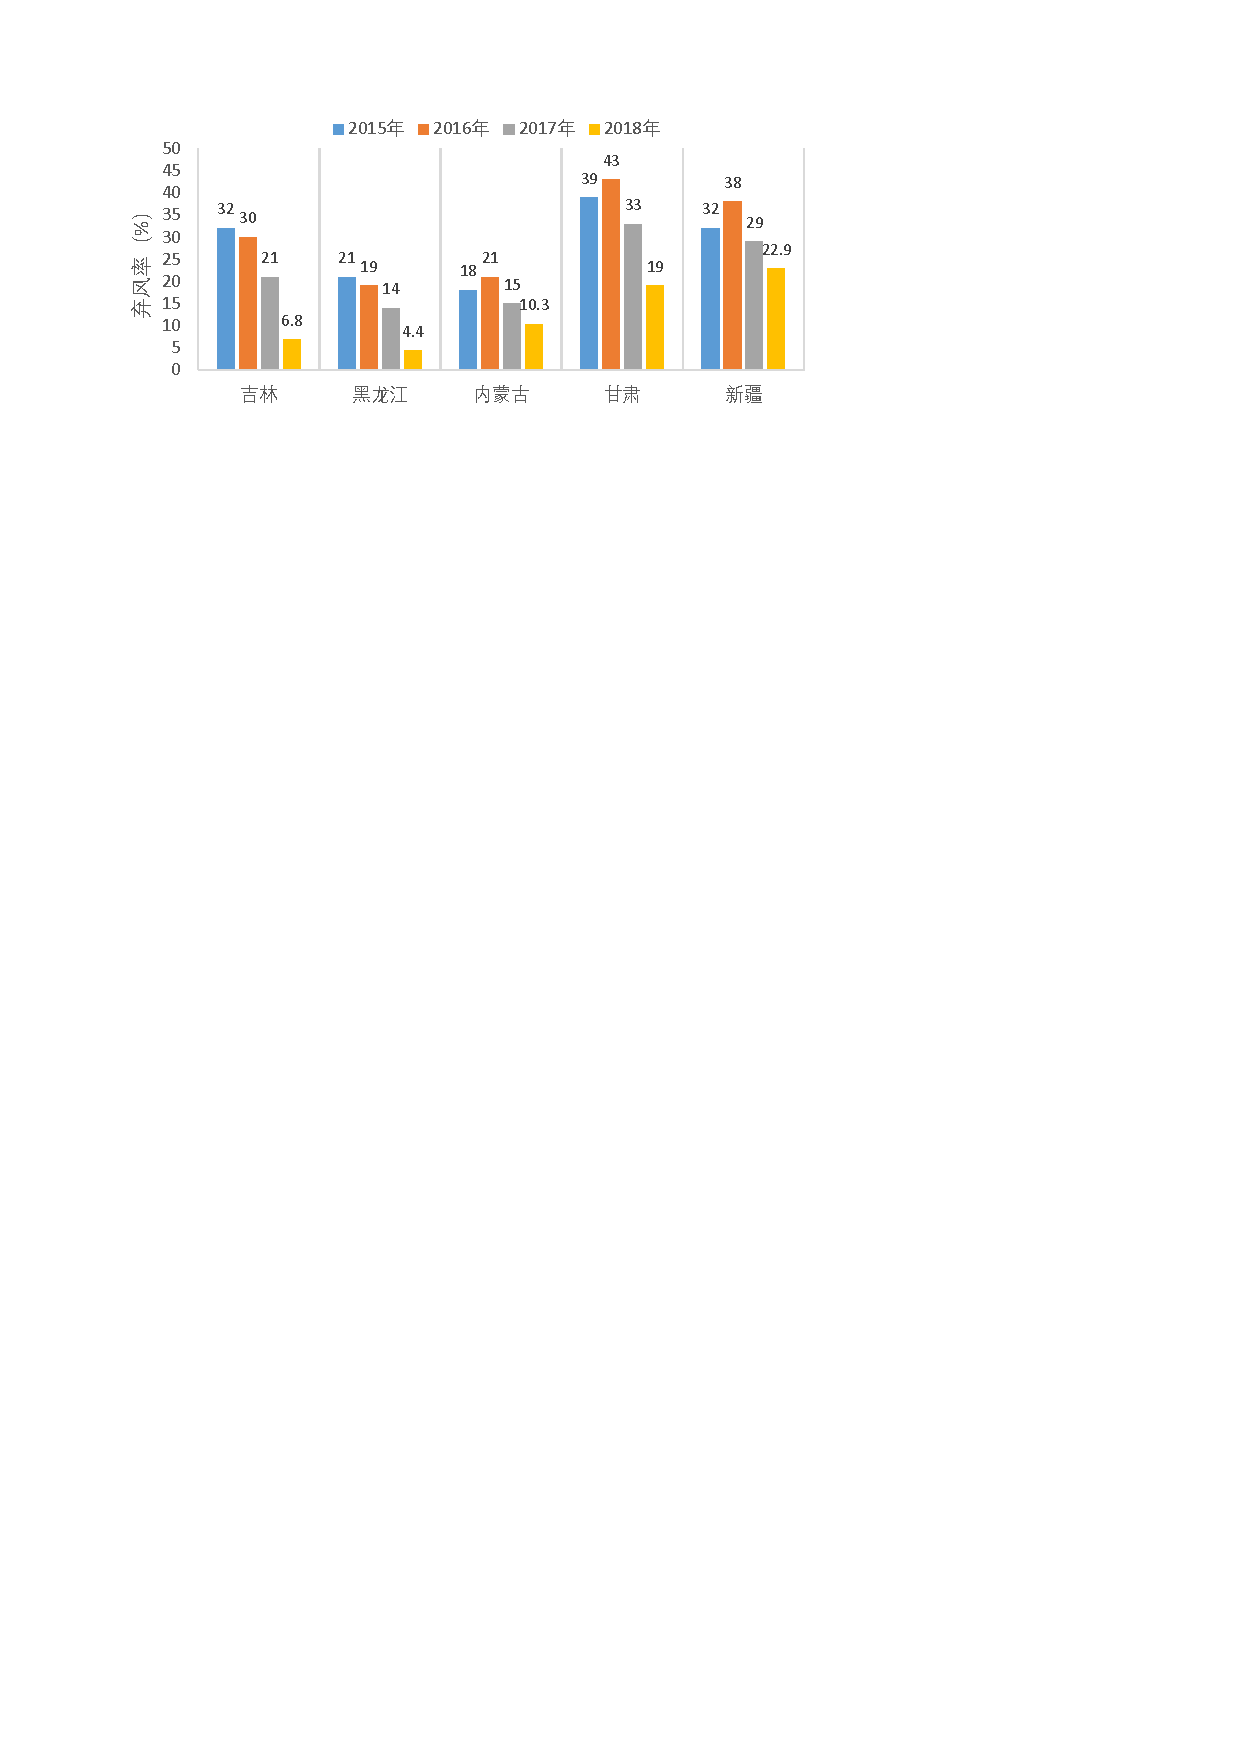
\includegraphics[scale=0.95]{figures/Chap1-1-Wind-Curtailment-Province.pdf}
  \caption{典型省份弃风数据(2015-2018)}
  \label{fig:Wind-Curtailment-Province}
\end{figure}

近年来,高比例可再生能源电力系统的发展遇到一定挑战,主要表现为新能源电力高比例并网导致的消纳难题与负电价现象。受限于能源结构中煤炭占比高与灵活调节电源容量少等因素~\cite{Renewable-Consum-17},我国西北、东北等可再生能源装机容量渗透水平较高地区,弃风问题较为严重。2016年,吉林、黑龙江弃风分别达30\%与19\%,内蒙古弃风达21\%,甘肃与新疆弃风分别达43\%与38\%,如图~\ref{fig:Wind-Curtailment-Province}~所示\footnote{数据整理自国家能源局历年新能源并网报告,http://www.nea.gov.cn}。通过可再生能源优先发电、可再生能源电力参与市场化交易、可再生能源电力配额制、省间跨区协调、负荷电气化等措施的逐步实施\footnote{国家能源局《解决弃水弃风弃光问题实施方案》, 国家电网《促进新能源发展白皮书》(2018)。},2017 年吉林、黑龙江弃风分别降为21\%与14\%, 内蒙古弃风降为15\%, 甘肃与新疆分别降为33\%与29\%;2018年吉林、黑龙江弃风分别降至6.8\% 与4.4\%, 内蒙古降至10.3\%,甘肃与新疆电网弃风分别降至19\%与22.9\%。尽管弃风问题有了一定程度的改善,但受限于新能源电力系统本身灵活性资源的缺乏,系统能继续接纳的新能源(容量与电量)比例受限,维持较低的弃风水平的前提是风电装机容量的缓慢增长,如图~\ref{fig:Wind-Installment-Capacity}~所示\footnote{图中数据整理自国家能源局, http://www.nea.gov.cn}。

\begin{figure}[H] % use float package if you want it here
  \centering
  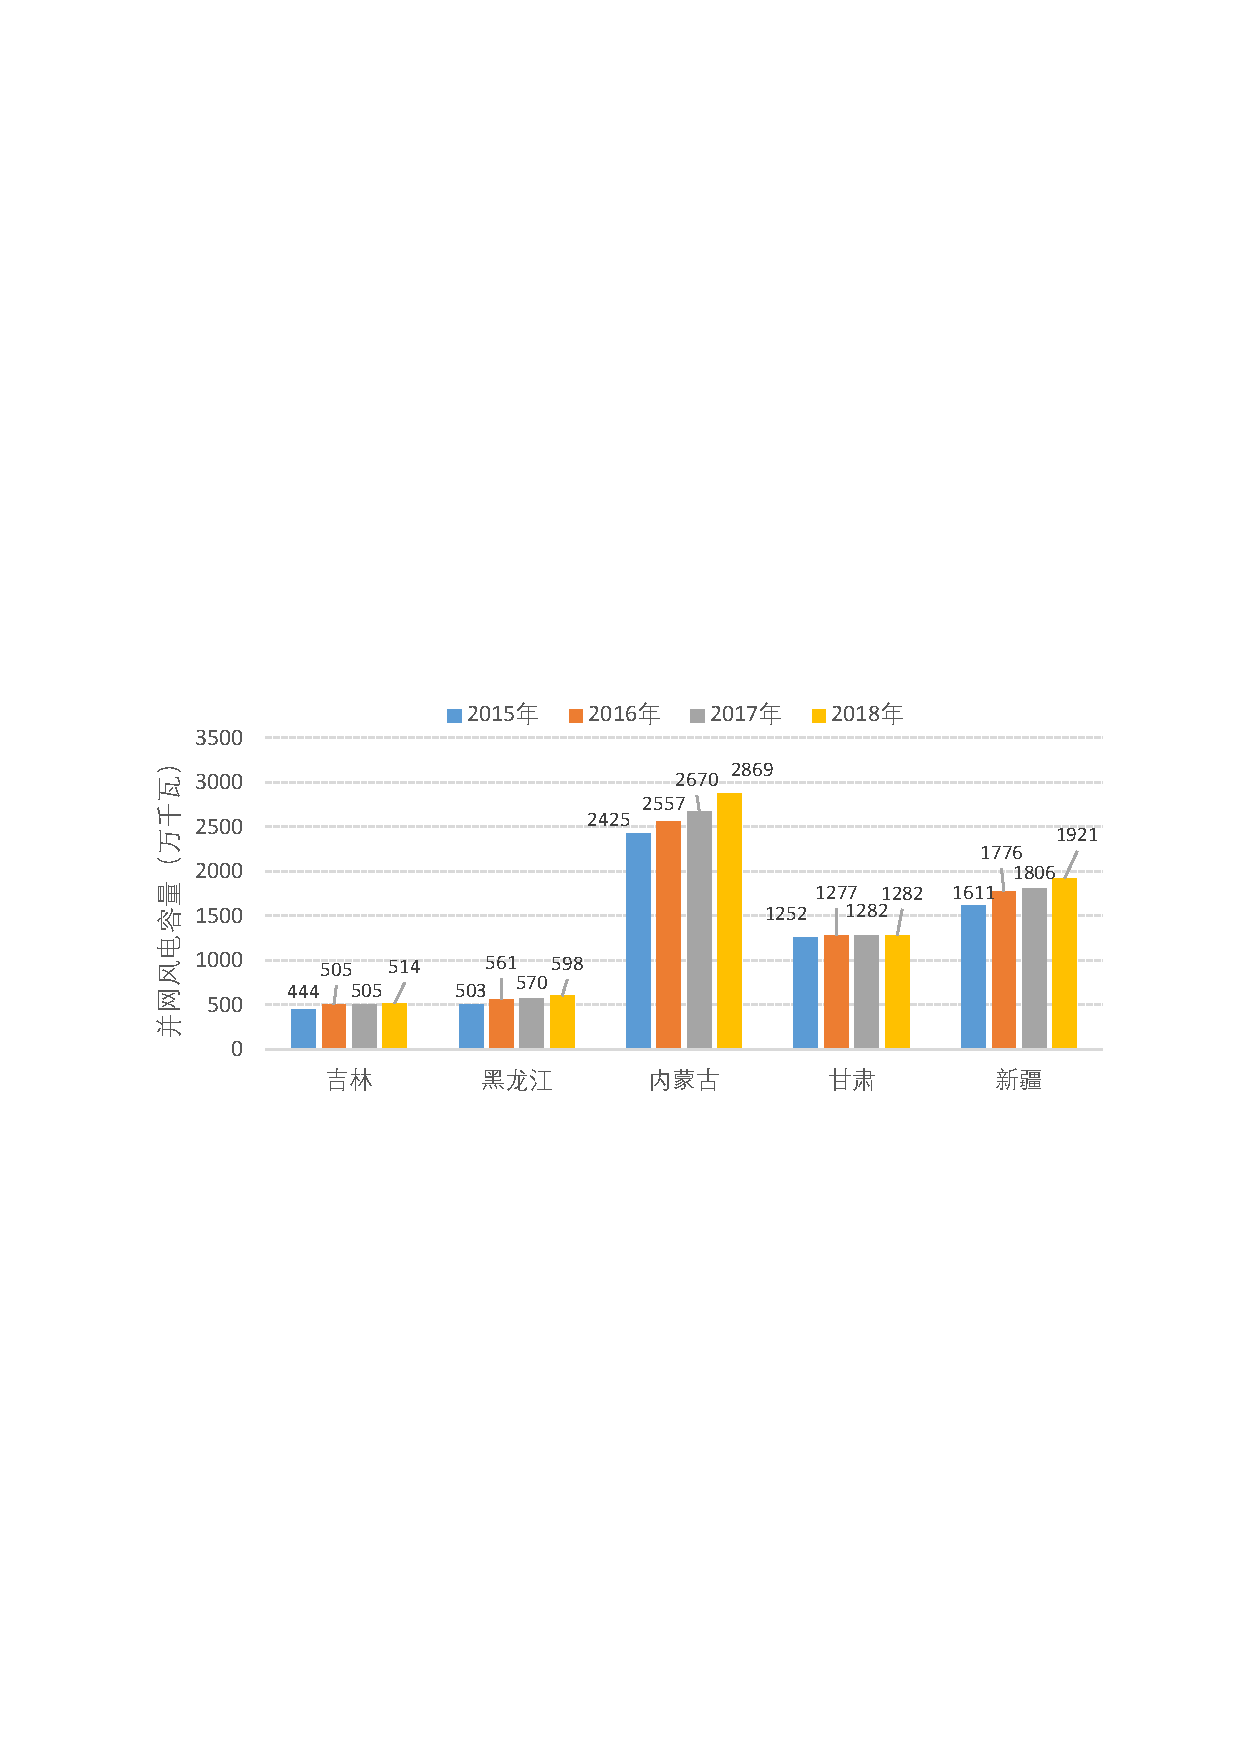
\includegraphics[scale=0.75]{figures/Chap1-1-Wind-Installment-Capacity.pdf}
  \caption{典型省份风电并网装机容量(2015-2018)}
  \label{fig:Wind-Installment-Capacity}
\end{figure}

受限于新能源电力的波动性与不确定性,美国、德国等国家出现了较为频繁的负电价现象, 且有愈演愈烈之势\cite{Neg-Price-US-Evidence,Neg-Price-German-13}。以可再生能源资源丰富的美国加州CAISO 电力批发市场为例,SP-15节点2014年负电价小时数占比为5.03\%, 2015年升为5.40\%, 2016 年升至8.33\%\cite{Neg-Price-US-Evidence}。类似地,PJM、ERCOT、ISO-NE、NYISO等电力市场的负电价占比也在(持续)增长,如表~\ref{tab:neg-price-US}所示。新能源机组的不可调度性,使其难以响应(预测的)电力市场电价信号(负电价与峰谷价差等)并调整风电出力,从而影响了风电机组的运行经济性。辨识影响可再生能源电力发展的关键因素,是实现可持续的高比例可再生能源电力供应的前提。

\begin{table}[htb]
  \centering
  \begin{minipage}[t]{0.8\linewidth} % 如果想在表格中使用脚注,minipage是个不错的办法
  \caption{美国电力市场典型节点负电价小时数占比变化(2013-2016)
  \footnote{表中数据整理自文献\inlinecite{Neg-Price-US-Evidence}。}}
  \label{tab:neg-price-US}
    \begin{tabularx}{\linewidth}{cccccc}
      \toprule[1.5pt]
      {\heiti 年份} & {\heiti CAISO} & {\heiti ERCOT} &  {\heiti NYISO} & {\heiti PJM} & {\heiti ISO-NE} \\\midrule[1pt]
      2013 &	2.26\%	& 0.29\%  & 1.37\%	& 2.41\%  & 0.00\%  \\
      2014 &	5.03\%	& 0.67\%  & 2.13\%	& 5.24\%  & 0.76\%  \\
      2015 &    5.40\%	& 3.79\%  & 8.56\%	& 11.00\% & 1.64\%  \\
      2016 &    8.33\%	& 3.94\%  & 6.54\%	& 4.01\%  & 2.77\%  \\
      电价节点 &	SP-15 & 	West & 	ZoneD-North &	Byron &	Maine\\
      \bottomrule[1.5pt]
    \end{tabularx}
  \end{minipage}
\end{table}

事实上,中国“三北地区”存在的新能源消纳难题与美国、德国等出现的负电价现象主要受新能源电力系统中电源、电网及负荷三侧的因素综合影响,具体表现在:1)受风/光资源与风/光功率间的瞬时强耦合关系,源侧并网的新能源电力具有较强的波动性与随机性,以及不可调度性;2)网侧的灵活调节容量、输送通道容量等因素的限制,难以为源侧注入的不确定性提供充足的灵活性资源~\cite{Renewable-Consum-17};3)荷侧聚焦于电能形式的消纳模式难以有效发挥终端热电协同调控对新能源电力系统灵活性资源的支撑作用~\cite{,EH-FREEDM-11,Smart-Grid-Energy-Internet-14,IES-Review}。

\subsection{压缩空气储能及支撑政策}
大规模储能(储电、储热)技术是平滑新能源出力波动性、提高输电通道平均利用率、提供灵活调峰容量及实现新能源电力热电协同调控的主要措施之一~\cite{Balance-Nature16,ESS-Engineering-15,TES-CSP-12,CAES-Review-18-Rui-operation}。为支撑2050 年可再生能源发展规划,美国、欧洲、中国等市场的储能容量总需求达450GW ~\cite{IEA-Report-14}。 目前已商业化的大规模物理储能技术主要包括抽水蓄能和压缩空气储能(Compressed Air Energy Storage, CAES)\footnote{本文设定CAES指代压缩空气储能技术,不涉及其具体实现方案,如等温、绝热及非绝热等。},前者约占全球~141GW(2017年)储能容量的99\%,但因建址条件及潜在生态环境等因素,发展已渐趋平缓~\cite{IEA-Report-14}。 近二十年来,CAES 因容量大、寿命长、响应速度快等优点得到了国内外多个大型企业及研究机构的关注,欧、美、日、中、加等也纷纷部署了CAES 技术发展路线~\cite{CAES-Review-16-Polygeneration,CAES-Review-09,CAES-Review-16-Rui,CAES-Review-17,CAES-Review-18-Rui-operation}。

先进绝热压缩空气储能(Advanced Adiabatic Compressed Air Energy Storage, AA-CAES)是一种通过空气压缩热能的回收再利用摒弃燃料补燃的新型CAES技术形式~\cite{ACAES-Green-12}, 其工作原理如图~\ref{fig:AA-CAES-principle-abs}~所示。压缩储能时, AA-CAES 利用弃风(光)、低谷电等电能或风能等机械能驱动压缩机,经绝热压缩(压缩系统)回收压缩热,解耦存储空气压力势能(储气库)和压缩热能(蓄热系统);膨胀释能时,通过绝热膨胀(透平系统\footnote{文献中透平系统亦称为膨胀系统,本文对二者不加区分。})利用压缩热能,实现空气压力势能和压缩热能的耦合释能\cite{CAES-Review-18-Rui-operation}。

与电池储能、抽水蓄能等储能技术不同,AA-CAES除了能提供常规储能具有的能量搬移与容量备用方面的灵活性~\cite{CAES-Baseload-Review-12,CAES-Reserve-11}外,还能为新能源电力系统注入供能灵活性及接口灵活性,主要表现在:1)蓄热系统(换热器与储热罐)的存在使AA-CAES 具备了潜在的热电联供与热电联储能力,其既可配置于电力系统电能单能流应用场景,也可应用于区域热电综合能源系统热电多能流场景,具有一定的供能灵活性~\cite{CAES-Review-18-Rui-operation,CAES-Review-16-Polygeneration}; 2)AA-CAES可以风能等机械能作为输入接口直接驱动,亦可以输出机械能直接驱动动力机械等,具有良好的接口灵活性,有望实现风-储集成设计,进而从源头上改善风电功率的波动性。

\begin{figure}[H] % use float package if you want it here
  \centering
  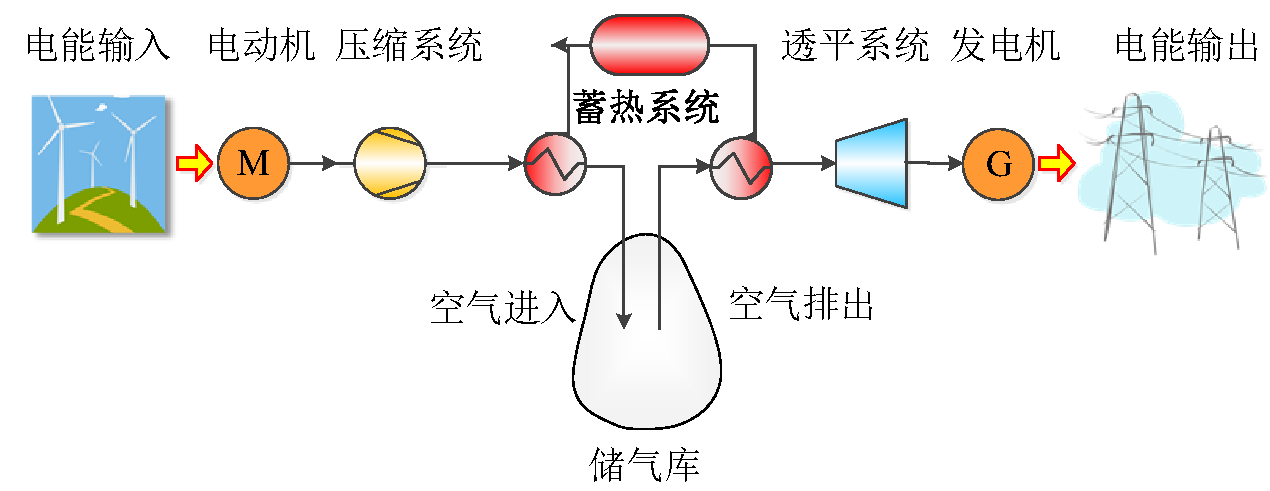
\includegraphics[scale=0.60]{figures/Chap1-1-AA-CAES-Principle-Abs.pdf}
  \caption{AA-CAES工作原理示意图}
  \label{fig:AA-CAES-principle-abs}
\end{figure}

AA-CAES具有的常规、供能、接口等三类灵活性可为从源—网—荷三侧支撑可持续的高比例可再生能源电力供应提供新的思路,也因此成为目前CAES 领域的主流技术~\cite{AA-CAES-04,AA-CAES-07},备受我国能源电力部门的青睐。2016年6月,CAES技术被纳入《中国制造2025—能源装备》计划;与此同时相关储能支撑政策不断出台,加快了储能示范项目的商业化进程~\cite{ESS-CESA-16,ESS-CIAPS-16,CAES-Review-18-Rui-operation}。《关于推进电能替代的指导意见》
\footnote{http://www.ndrc.gov.cn/gzdt/201605/t20160524$\_$804439.html} 鼓励拉大峰谷价差,以提高储能经济性;《关于促进电储能参与“三北”地区电力辅助服务补偿(市场)机制试点工作的通知》
\footnote{http://zfxxgk.nea.gov.cn/auto92/201606/t20160617$\_$2267.htm} 鼓励储能设施参与辅助服务市场,进一步创造储能收益源;《关于促进储能技术与产业发展的指导意见》
\footnote{http://www.nea.gov.cn/2017-10/11/c$\_$136672015.htm},描绘了储能10 年发展蓝图——“十三五”期间进入商业化初期,“十四五”期间实现规模化发展;《关于进一步深化电力体制改革的若干意见(中发[2015]9号)文》
\footnote{http://www.nea.gov.cn/2015-11/30/c$\_$134867851.htm} 及系列配套文件为建立健全辅助服务市场及储能参与辅助服务提供了市场条件\cite{CAES-Review-18-Rui-operation}。

\subsection{研究意义}
随着压缩机、换热器、储气库、储热及透平膨胀机\footnote{文献中透平膨胀机存在多种名称,包括膨胀机、空气透平及空气透平膨胀机等,本文不加以区分。}等关键技术的突破~\cite{CAES-Review-17-Rui-salt,TES-CSP-review-13},以及国内外多项示范工程的逐步落实与有序推进,AA-CAES将从平滑新能源电力的波动(源侧)、提供灵活调节容量(网侧)及支撑热电协同调控(荷侧)等方面促进可再生能源电力的可持续高比例接纳。

在电能单能流应用场景下,AA-CAES 可配置在风电光伏场站侧,形成风光/储混合系统承担系统基荷,缓解输电线路阻塞、提高输电线路载荷率、延缓输配线扩容;亦可部署于负荷侧支撑电网削峰填谷,实现能量的时空平移,消纳可再生能源电力承担系统峰荷\cite{CAES-Review-18-Rui-operation}。在热电多能流应用场景下,AA-CAES可作为能量枢纽充当终端冷热电三联供设备,发挥多能互补协同效应,促进可再生能源的高效消纳\cite{CAES-Review-18-Rui-operation}。此外,AA-CAES亦可与风机实现机械接口的集成设计,减弱风功率输出与风速间的瞬时强耦合关系,从源头上改善风电的波动性与不确定性,从而有望降低新能源电力系统对灵活性资源的需求。

AA-CAES在源—网—荷侧各应用场景的成功应用与推广,离不开对其组件热力学特性、建模设计、调度运行及市场运营理论与方法的研究。本文直面新能源电力系统中的AA-CAES 技术,聚焦于面向各类典型应用场景的AA-CAES高效设计、灵活性建模、调度运行及市场运营等问题,以期从源—网—荷三侧助力可再生能源电力的可持续高比例接纳。

\section{国内外研究现状}
\label{sec:research-state}
%\subsection{可持续性100\%清洁能源供应系统}
\subsection{压缩空气储能概念发展与工程示范}
\label{sec:research-state-engineer}

\subsubsection{概念发展}
自1949年~Stal~Laval~公布首个专利至今, ~CAES~技术已存在多种实现形式, 主要包括非绝热型(Diabatic CAES, D-CAES)、绝热型(Adiabatic CAES, A-CAES)及等温型(Isothermal CAES, I-CAES)等。其中,D-CAES 在透平发电过程采用天燃气等燃料补燃,而A-CAES 采用压缩过程收集的压缩热能代替D-CAES中的燃料补燃环节,I-CAES则通过在压缩储能与膨胀释能过程中注入水雾等实现空气的等温压缩与等温膨胀。此外, CAES还存在多种混合动力循环\cite{Thesis-Zhangjunliang,Thesis-Liuxiao}。

A-CAES可视为一种“局部准绝热、整体准等温”的CAES技术\cite{Thesis-Zhangxuelin},是当前~CAES~技术研究与工程示范的主流趋势。考虑到 A-CAES 的清洁特性及I-CAES尚未成熟等因素,本文重点关注A-CAES。事实上,A-CAES技术的发展历程与整个储能行业发展趋势类似,在不同的历史阶段触发于特定的应用需求,也因此在电力系统中也发挥着不同的功能,如图~\ref{fig:CAES-History}~ 所示。

\begin{figure}[H] % use float package if you want it here
  \centering
  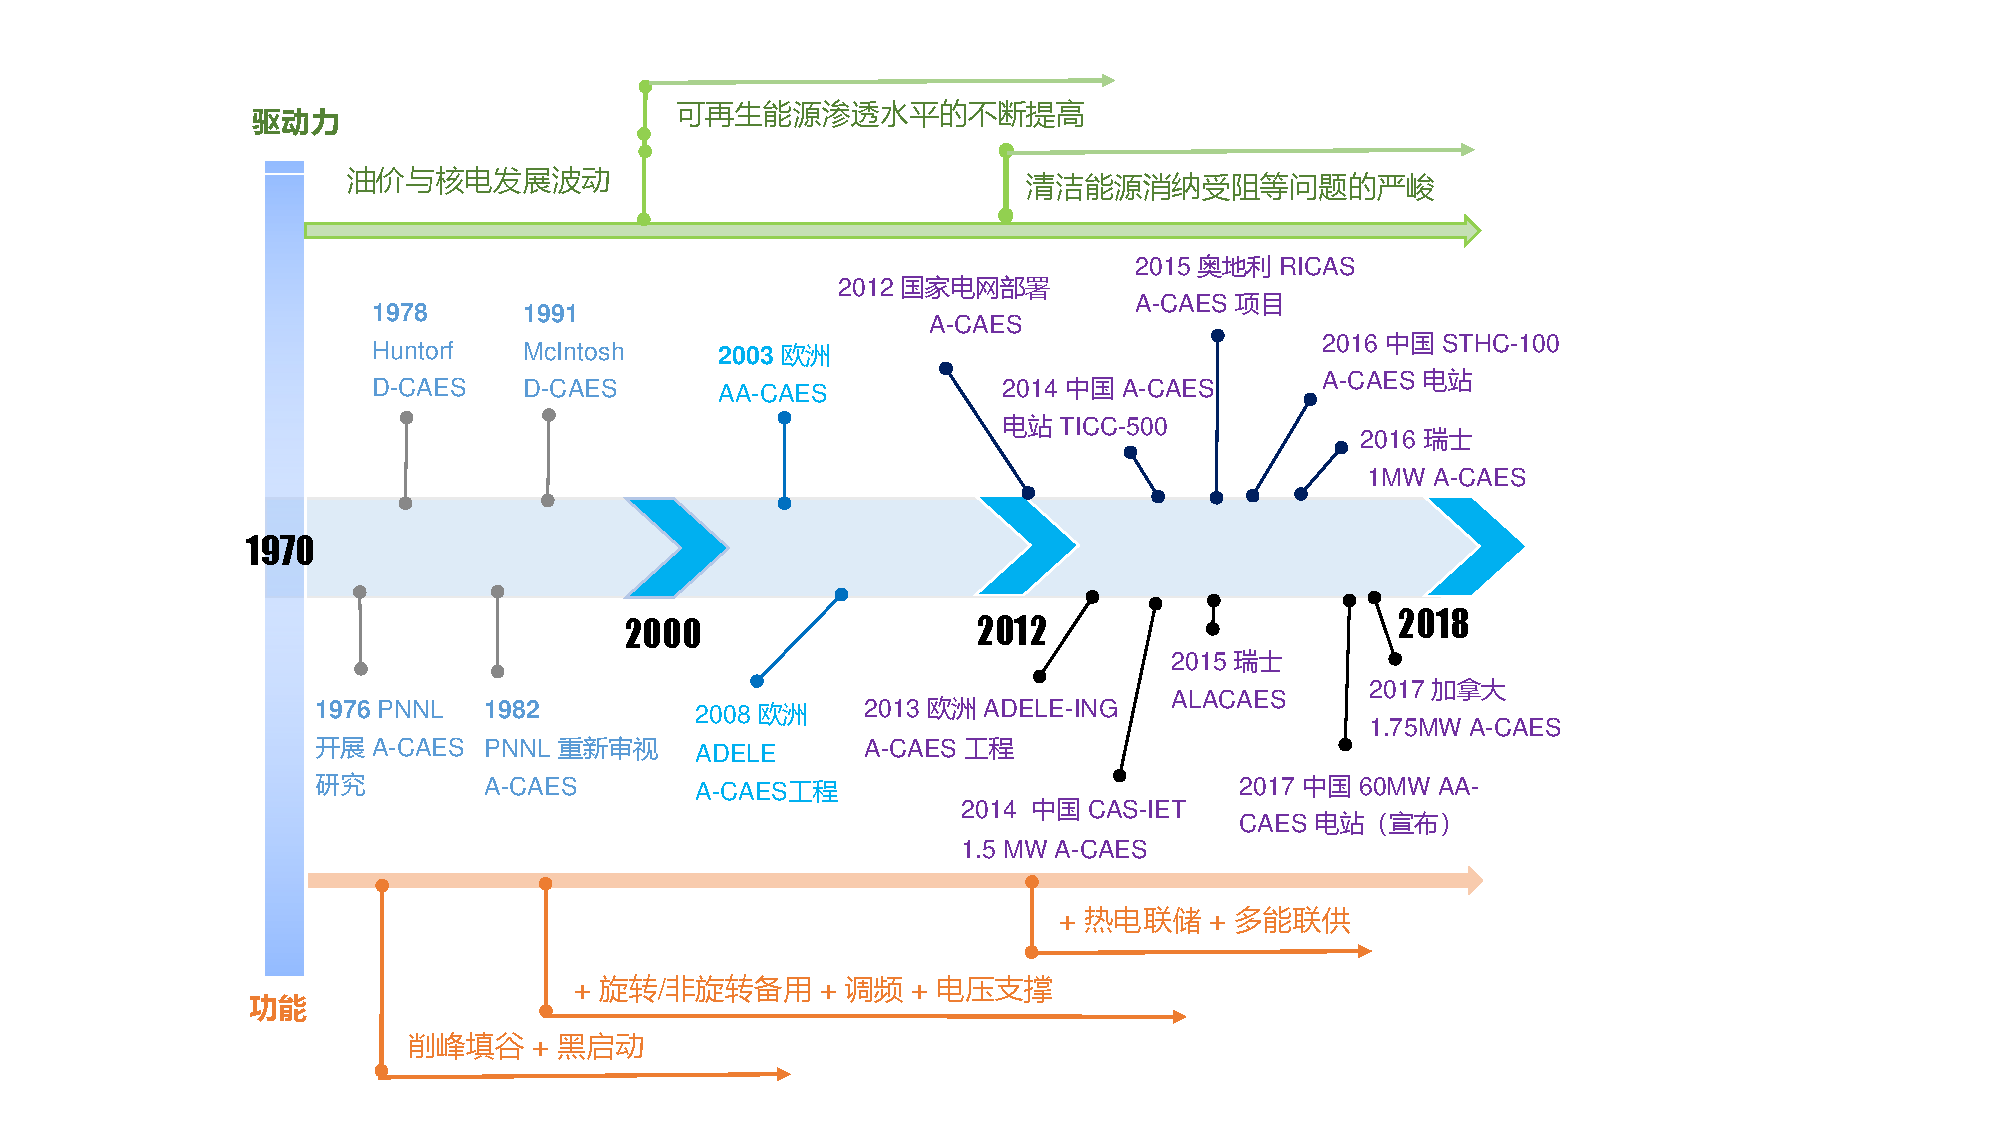
\includegraphics[scale=0.60]{figures/Chap1-4-CAES-History.pdf}
  \caption{A-CAES技术发展沿革(1970-2018)}
  \label{fig:CAES-History}
\end{figure}

二十世纪七八十年代,在国际燃气价格上升与燃气调峰机组经济性降低的背景下,欧洲、美国率先开展~D-CAES~技术研究,先后建成德国Huntorf (1978 年)和美国McIntosh (1991 年)两座商业电站,用来参与系统调峰和电源备用(黑启动),二者循环效率远高于燃气调峰机组,至今仍运行良好~\cite{IEA-EES-09,EES-Review-12,CAES-Review-18-Rui-operation}。然而, D-CAES 电站在释能发电过程需借助燃料补燃实现高效循环,存在化石燃料依赖、碳排放等问题~\cite{ACAES-Green-12,CAES-Huntorf-12},使其在天然气资源匮乏地区及当前可再生能源电力系统中的应用受限\cite{CAES-Review-18-Rui-operation}。

1976 年,美国西北太平洋实验室(Pacific Northwest National Laboratory, PNNL)开展A-CAES技术研究,指出了A-CAES 摒弃燃料补燃的技术经济优势~\cite{CAES-Review-18-Rui-operation,CAES-Patent-78,Thesis-Zhangyuan};1982 年,PNNL等进一步研究明确了在众多~CAES 技术中~A-CAES~的发展潜力~\cite{A-CAES-Report-81,A-CAES-Report-82}。然而,受限于储热技术的成熟度及高成本~\cite{AA-CAES-04},A-CAES~电站的建设成本和技术难度高于~D-CAES~电站~\cite{Thesis-Zhangyuan},致使~McIntosh~电站采用了~D-CAES~技术方案。

21世纪初,环境气候的严峻挑战与新能源电力的并网消纳需求,唤醒了~A-CAES~技术的研究热潮~\cite{AA-CAES-04}。 储热技术的逐步成熟及其在集中式光热等领域的成功应用~\cite{TES-CSP-review-13},使得多个国家和地区聚焦于新一代~A-CAES~技术,即~AA-CAES~技术的研究与工程示范\footnote{我们认为,~A-CAES~技术与~AA-CAES~技术并无本质区别,为便于叙述,后文均以~AA-CAES~一并表示。}。特别地,自2012年起,随着新能源电力消纳受阻等问题的严峻,AA-CAES的热电联供与热电联储特性也逐渐得到关注。

\subsubsection{工程示范}
立足国内,多项~AA-CAES~示范工程有序推进,部分试验系统已开花结果\cite{CAES-Review-18-Rui-operation}。2012年10月,在国家电网支持下,清华大学联合中科院理化所、中国电力科学研究院开展AA-CAES 关键技术研究\cite{CAES-Review-17-Rui-salt}。2014 年3 月,中科院工程热物理研究所建成河北廊坊1.5MW先进CAES的集成实验系统,完成了~600~小时试验运行和性能测试\footnote{http://www.cas.cn/ky/kyjz/201404/t20140403\_4085514.shtml};同年12月,清华大学建成安徽芜湖 500kW AA-CAES实验系统TICC-500,在国内率先实现储能发电,电换电效率达41\%(初期实验效率33.3\%),综合能量效率达72\%~\cite{CAES-Review-18-Rui-operation,TICC-15,TICC-16}。2016 年8 月,清华大学在青海大学智慧微能源网示范园区投运100kW光热复合CAES试验系统STHC-100,并初步完成冷热电三联供试验~\cite{ST-CAES-17,ST-CAES-CN-16-Rui,CAES-Review-18-Rui-operation};同年12 月,中科院工程热物理研究所开展贵州毕节10MW级AA-CAES系统集成实验与研发平台的联合调试\footnote{http://www.etp.ac.cn/xwdt/kydt/201612/t20161213$\_$4720289.html}。2017年5月,国家能源局批复立项我国首个AA-CAES国家示范电站——江苏金坛盐穴压缩空气储能发电系统~\cite{CAES-Review-17-Rui-salt};同年7月,国家能源局批复立项我国首个以AA-CAES为核心的“互联网+” 智慧能源示范项目—— 无为高沟电缆基地智能微电网\cite{CAES-Review-18-Rui-operation}
\footnote{http://www.nea.gov.cn/136106972$\_$14887900533341n.pdf}。2018年3 月,国家能源局《2018 年能源工作指导意见》指出,“积极推进江苏金坛压缩空气储能项目,研究推进100MW压缩空气储能电站”;2018年12月,金坛压缩空气储能项目开工建设\footnote{http://www.escn.com.cn/news/show$\_$696396.html}。

放眼国际,德国、美国、加拿大、奥地利、瑞士等国纷纷宣布、设计或建设多座AA-CAES电站~\cite{CAES-Review-16-Polygeneration,CAES-Review-09,CAES-Review-16-Rui,CAES-Review-18-Rui-operation}。2003 年,欧盟委员会资助~AA-CAES~项目,旨在评估面向集中式、分布式及孤岛等应用场景的AA-CAES技术方案,并构建具有经济吸引力的概念型电站~\cite{AA-CAES-04}。2008 年,德国莱茵集团等启动~ADELE~ 项目,开展~AA-CAES~技术的可行性论证、概念设计及组件研发等工作~\cite{AA-CAES-07};2013年,莱茵集团进一步启动~ADELE-ING~项目,研究~AA-CAES~技术的工程特性并评估不同的系统方案\footnote{http://www.sccer-hae.ch/resources/SymposiumMay2015/Talks/SCCER2015-AdiabaticCAES-Zunft.pdf},筹划建设~ADELE~ 示范电站,设计容量达300MW/1000MWh,预计循环效率达66\%-70\%\footnote{2017年12 月,由中国盐业公司、清华大学等单位组成的考察团赴德国调研表明,该项目目前已被终止。}\cite{CAES-Review-18-Rui-operation}。 2013 年,美国PNNL 评估了Yakima 结合地热和盐穴储气的~AA-CAES~方案~\cite{AA-CAES-Patent-12} 及其技术经济性~\cite{CAES-PNNL-13}。2015 年,奥地利启动 RICAS2020 项目评估~AA-CAES~技术的性能与可行性,并聚焦于研发较具经济性的地下储气方案,同时构建移动式~AA-CAES~系统~\footnote{https://www.sintef.no/en/projects/ricas-2020-design-study-for-advanced-adiabatic-com/}\cite{CAES-Review-18-Rui-operation}。 瑞士~ALACAES~公司致力于研发面向~AA-CAES~的储热技术,采用隧道和洞穴储气方案评估了~AA-CAES~ 技术的环境经济潜力,于~2016~年在瑞士比亚斯卡建成了一座~1MW/MWh AA-CAES~示范系统~\footnote{https://alacaes.com/}\cite{CAES-Review-18-Rui-operation},并在文献~\inlinecite{AA-CAES-Demo-ALACAES-1,AA-CAES-Demo-ALACAES-2}中基于储热系统的实测数据及其它组件的预估性能,得出了63\%-74\%的电-电循环效率。2017 年5月,加拿大~NRStor~和~Hydrostor~公司开始联合研发大规模~AA-CAES~技术,目前正在加拿大戈德里奇建设一座基于盐穴储气~1.75MW/7MWh~AA-CAES试验电站~\footnote{https://www.energy-storage.news/news/canadian-firms-nrstor-and-hydrostor-partner-up-on-utility-scale-adiabatic-c}\cite{CAES-Review-18-Rui-operation}。

毋庸置疑,上述工程实践极大加强了面向新能源电力系统源、网、荷侧各应用场景的AA-CAES设计、建模、运行及运营等理论与方法的研究需求, 而分析AA-CAES独特的灵活性特点则是开展相应研究工作的前提。

%\subsection{新型灵活压缩空气储能系统}

\subsection{压缩空气储能系统的三类灵活特性}
\label{sec:flexibility-intro}
前已提及,独特的热力循环与设计理念赋予了AA-CAES多种灵活性,具体包括:1)以能量搬移与容量备用为核心的常规灵活性;2)以热电联供与热电联储为特点的供能灵活性;3)以机械输入与机械输出为内涵的接口灵活性。AA-CAES的常规、供能及接口等三类灵活性,为从源、网、荷三侧促进高比例可再生能源电力的可持续供应提供了新视角。

\subsubsection{常规灵活性:能量搬移与容量备用}
CAES的大容量特性及优良的动态特性使其具备了长时间的能量储存与搬移功能,以及良好的容量备用等灵活性支撑能力。实际运行表明,D-CAES电站具有启动速度快、爬坡率高、工作范围宽及运行模式灵活等优点\cite{CAES-Review-18-Rui-operation}。具体表现为:1)快速启动能力,3min—5min 可达70\%膨胀发电容量,10min 内实现满功率发电,5min 内实现满功率压缩~\cite{Huntorf-20-01};2)高爬坡率,如McIntosh 电站爬坡率约为18MW/min, 高于典型燃气轮机约60\%~\cite{CAES-Alabama-06};3)宽工况运行能力,如McIntoch 电站透平机械设计及控制方案提供方Dresser-Rand 公司拥有的SMARTCAES在发电和压缩环节均可实现25\%-100\% 负载运行\footnote{http://www.dresser-rand.com/industries/energy-environment/compressed-air-energy-storage/};4)灵活的运行模式,既可以超前功率因数运行的电动机模式压缩储能和提供无功,亦可以单位或滞后功率因数运行的发电机模式膨胀释能,抑或是以同步调相模式提供动态无功支撑~\cite{CAES-Reactive-13,CAES-Reactive-18-LGK}。 上述优良动态特性使~D-CAES~电站具备了调频、备用、无功调节及黑启动等功能,可为电网相关服务提供灵活性支撑,也为D-CAES电站的市场运营提供了多个收益源,有利于提高其竞争力与经济性\cite{CAES-Review-18-Rui-operation}。

\begin{figure}[htp] % use float package if you want it here
  \centering
  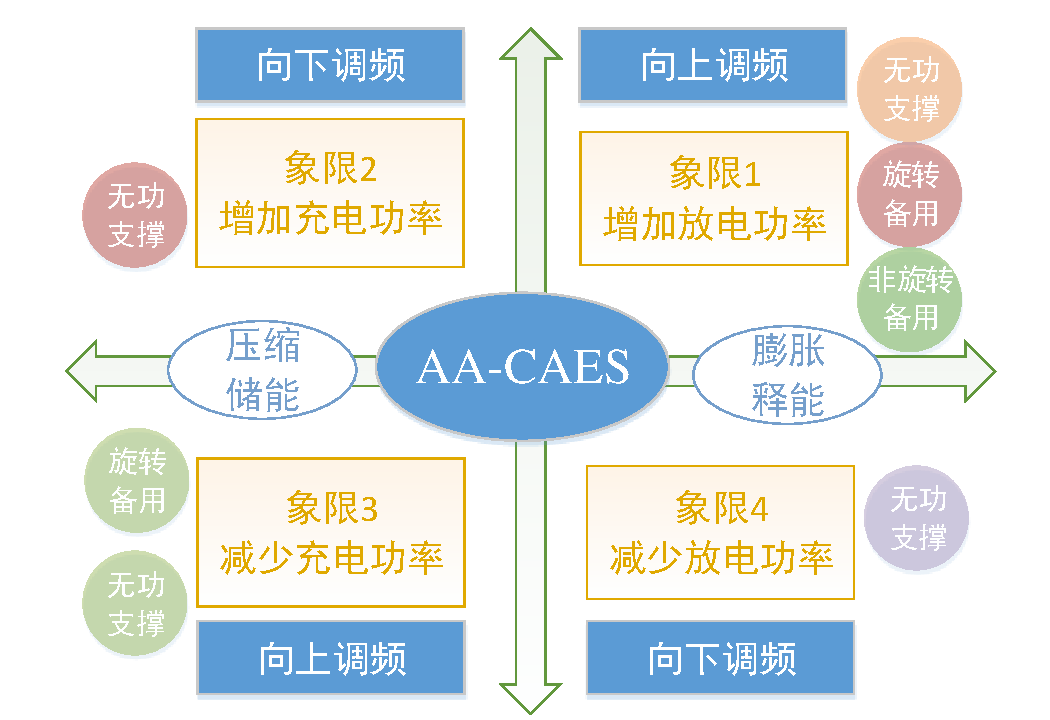
\includegraphics[scale=0.60]{figures/Chap1-2-CAES-AS-Overview-2.pdf}
  \caption{AA-CAES 辅助服务功能示意图}
  \label{fig:CAES-AS-Overview}
\end{figure}

不同于D-CAES电站,AA-CAES采用蓄热系统代替燃料补燃,压缩机与膨胀机一般不共轴\footnote{D-CAES一般采用共轴方案的原因在于其设计理念源于内含共轴压缩机与膨胀机的燃气轮机。},从而能够减少压缩、停机(静置)、膨胀模式间的切换时间,提高了压缩环节的响应速度\cite{CAES-Review-18-Rui-operation},具有比常规D-CAES电站更为优良的调频、旋转备用等辅助服务特性~\cite{ESS-Model-14},如图~\ref{fig:CAES-AS-Overview} 所示。以调频为例,当电网频率下跌时,AA-CAES电站可通过增加膨胀(发电)功率或减少压缩(充电)功率为系统提供向上调频容量;当电网频率过高时,AA-CAES 电站可通过减少膨胀功率或增加压缩功率为系统提供向下调频容量\cite{CAES-Review-18-Rui-operation}。同时,AA-CAES电站在压缩储能与膨胀释能过程中均可为电网提供旋转备用容量,在膨胀释能过程中还可提供非旋转备用容量\cite{CAES-Review-18-Rui-operation}。此外,AA-CAES电站在压缩和膨胀过程中的无功支撑能力使其能为电网提供一定的无功支撑 \cite{CAES-Reactive-18-LGK}。

需要说明的是,1)与电池储能不同,AA-CAES的调频、备用容量等将受到其蓄热系统、储气系统及供能特性的影响\cite{AA-CAES-Reserve-LYW-18};2)由于蓄热系统(及换热器)的传热动态一般比燃烧过程慢,采用蓄热系统代替天然气补燃环节后可能会降低AA-CAES在膨胀释能过程的响应速度\footnote{部分文献对此观点不一致,如文献\inlinecite{AA-CAES-Reserve-LYW-18}认为蓄热系统会比补燃环节更易提高响应速度。}\cite{CAES-Review-18-Rui-operation}。

\subsubsection{供能灵活性:热电联储与热电联供}
\label{sec:flexibility-poly-generation}
AA-CAES包含压缩机、膨胀机、换热器、蓄热系统、储气库等组件,各组件的热力学特性紧密耦合\cite{CAES-Review-18-Rui-operation}。换热器及蓄热系统的存在使AA-CAES电站可利用富余的压缩热能(或外部扩展热源)供热,具备了热电联供特性,提高了综合能量效率\cite{CAES-Review-18-Rui-operation}。AA-CAES电站的电能存储与热量存储特性赋予其热电联储能力,为其提供了良好的供能灵活性,适宜在分布式多能联供场景应用,如区域综合能源系统中实现热电协同调控~\cite{Trigen-mCAES-15,CAES-Alberta-14},进而提升新能源电力的渗透水平。

AA-CAES具备的结构层面的灵活扩展能力,可以增强其热电联储与热电联供能力。通过辅助电加热单元~\cite{Hybrid-CAES-14}、 光热收集单元~\cite{EH-CSP-17-Rui,Wind-Solar-CAES-12-Xu} 等外部扩展热源,扩展后的系统具有更强的热电联供与联储能力,提升了AA-CAES的供能灵活性。图~\ref{fig:ST-CAES-Hub} 给出了一种具有外部扩展热源的AA-CAES系统结构,可以实现灵活的热电联供与热电联储功能,是一种典型的热电清洁能量枢纽\cite{CAES-Review-18-Rui-operation}。文献~\inlinecite{ST-CAES-CN-16-Rui,ST-CAES-17,ST-CAES-CXT-18} 所构建的光热复合压缩空气储能系统即为一种采用槽式集热辅助单元的多能联供型AA-CAES能量枢纽。此外,文献~\inlinecite{High-Temp-CAES-17} 也给出了一种结合光热或低中温废热的AA-CAES 系统,在增强供能灵活性的同时,可以降低系统成本。

\begin{figure}[H] % use float package if you want it here
  \centering
  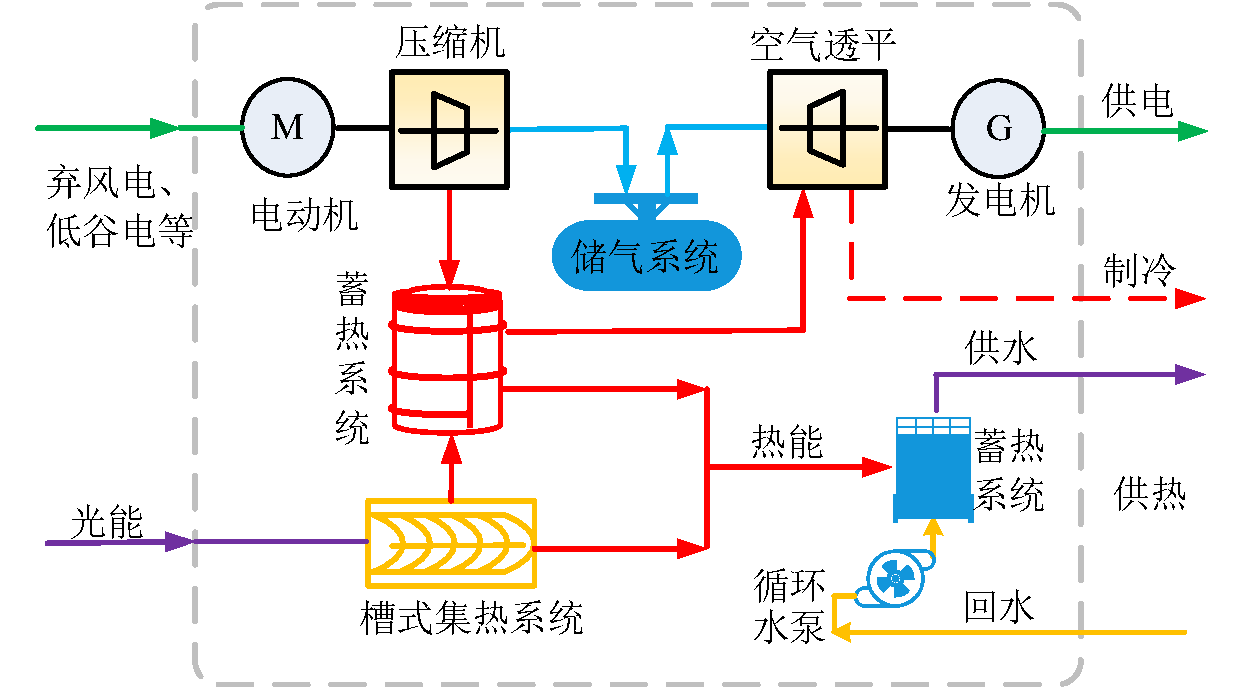
\includegraphics[scale=0.50]{figures/Chap1-3-ST-CAES-Hub.pdf}
  \caption{典型AA-CAES能量枢纽的结构}
  \label{fig:ST-CAES-Hub}
\end{figure}

事实上,AA-CAES可引入的电加热、光热等结构,本质上可视为接口灵活性。但是,本文关注的接口灵活性特指AA-CAES整体与新能源电力系统的机械能(非电)输入与机械能(非电)输出接口,而增设补热环节等改善AA-CAES 多能联供能力的结构灵活性被纳入供能灵活性。

\subsubsection{接口灵活性:机械输入与机械输出}
不难发现,图~\ref{fig:AA-CAES-principle-abs}中~AA-CAES~的输入与输出端分别采用电动机与发电机实现与电力系统的电能形式接口。事实上,我们可以直接采用风能等机械能驱动AA-CAES中的压缩机(省去压缩机前面的电动机),如文献~\inlinecite{Thesis-Zhangyuan,WT-CAES-Fea-15,CA-WT-16,Thesis-Zhangyi}设计的风-储集成系统;同时,也可直接利用AA-CAES 透平膨胀机输出的机械能(省去膨胀机后面的发电机),无需将其转化为电能,如法国MDI公司的压缩空气动力汽车AIRPod\footnote{MDI: Motor Development International.}。 如此,我们可以有效地利用风能直接驱动压缩机或直接输出机械能,实现风-储集成设计,从而有望降低风机存在的风速与风电输出功率之间的瞬时强耦合性以及新能源电力系统对灵活性资源的需求。本文将AA-CAES的这一灵活特性称之为接口灵活性。相比于AA-CAES,电池等其它储能技术必须以电能输入与电能输出作为其与电力系统的接口,其灵活性较差。

\begin{figure}[htp] % use float package if you want it here
  \centering
  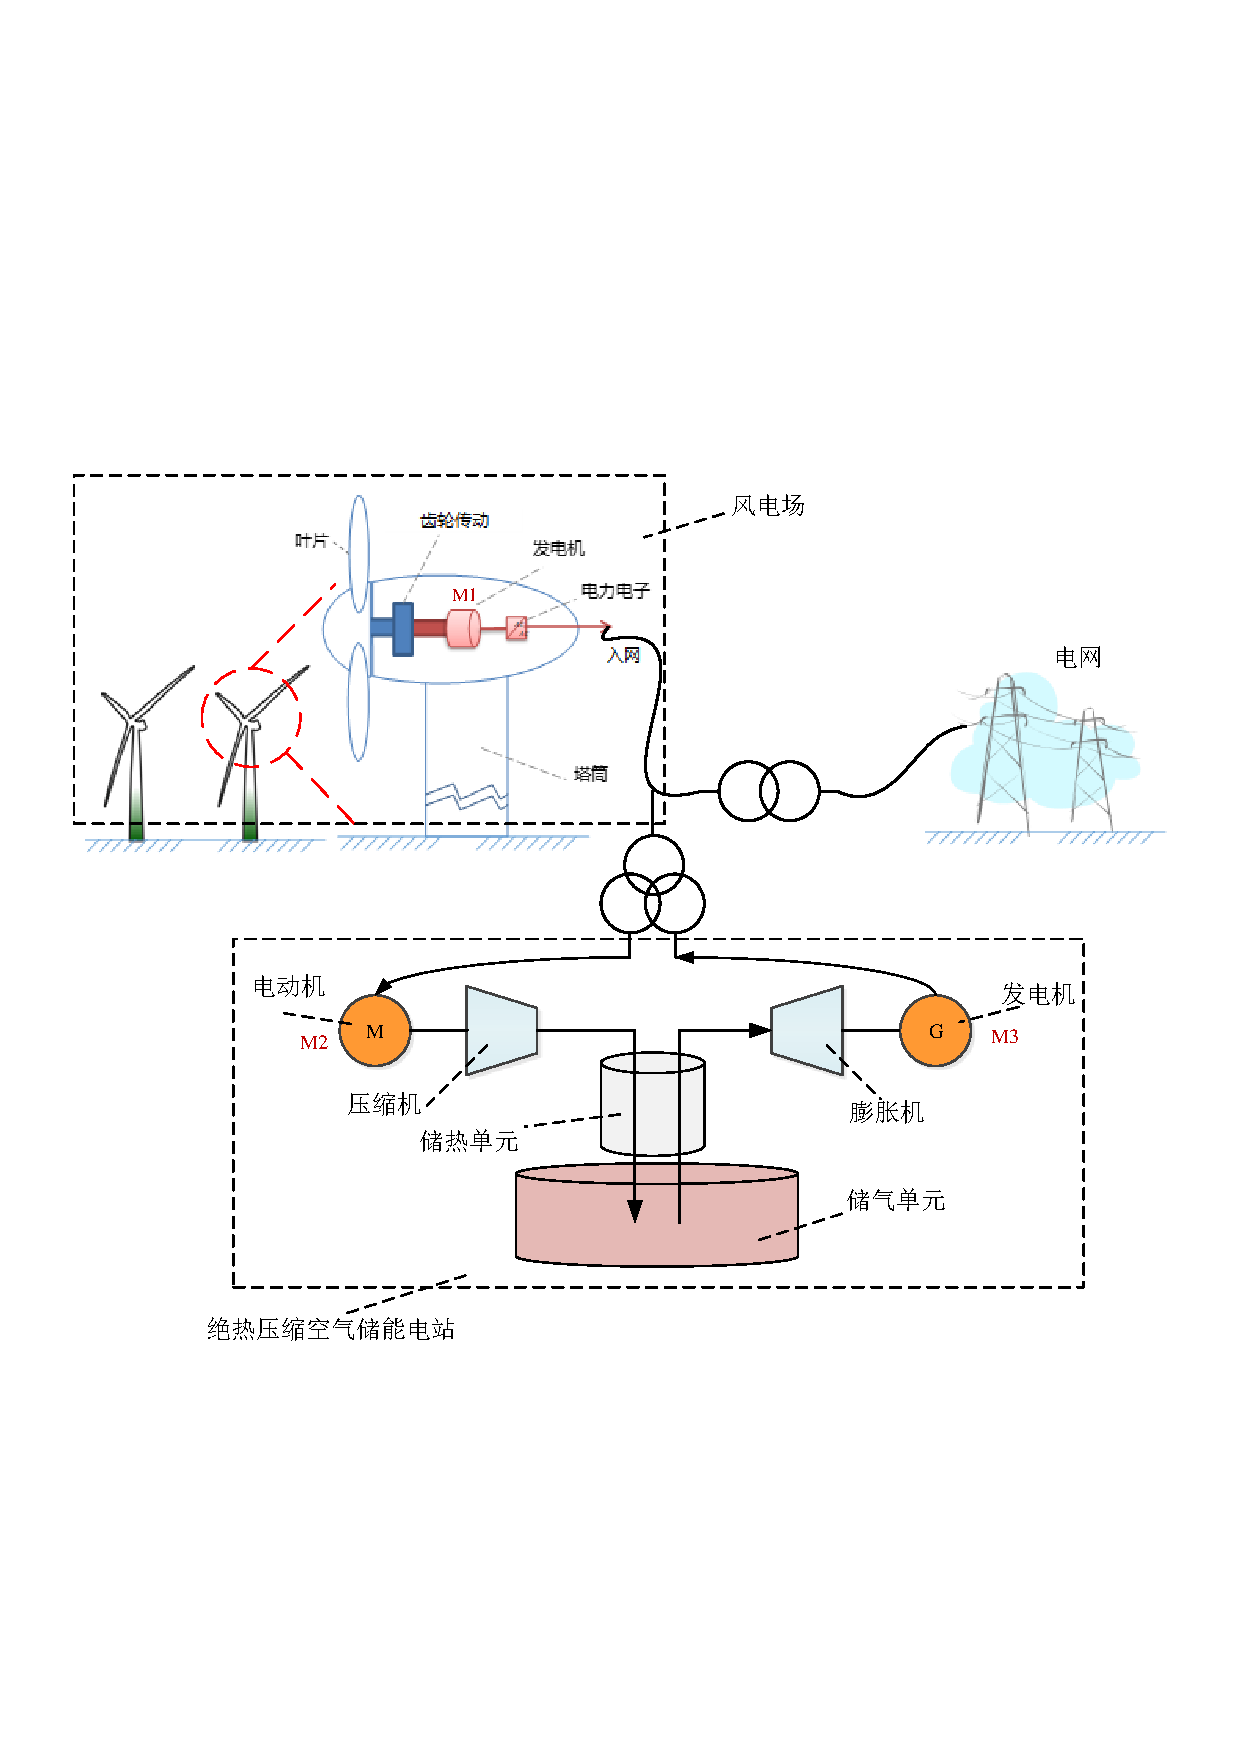
\includegraphics[scale=0.75]{figures/Chap1-5-AA-CAES-Stru-Flex.pdf}
  \caption{风-储协同系统中的AA-CAES接口灵活性示例}
  \label{fig:AA-CAES-Stru-Felixibity}
\end{figure}

以图~\ref{fig:AA-CAES-Stru-Felixibity}~所示的风电场与储能(AA-CAES)混合系统的经典配置结构为例, 我们分析需挖掘接口灵活性的典型场景。由于AA-CAES储能电站的压缩机及膨胀机需分别配设电动机与发电机,风-储混合系统一般至少含有三个电机~M1-M3。然而,三个电机均存在一定程度的容量浪费问题,具体地:1)风机内部的发电机M1 因可利用风能的大小在风速低于风机额定风速时存在着不同程度的容量浪费问题(风速越低问题越严重);2)M2在AA-CAES膨胀释能过程与静置时存在100$\%$ 的容量浪费;3)M3在AA-CAES压缩储能过程与静置时存在100$\%$的容量浪费;4)在风电上网不受限时段,由于AA-CAES储能系统无需运行,M2与M3完全静置。换言之,风-储(AA-CAES)混合系统中M2与M3的利用率远低于应用于负荷侧从电网进行储能的AA-CAES电站。若能挖掘AA-CAES的接口灵活性,直接采用风机叶片的(富余)机械能驱动压缩机以及采用膨胀机(与风机叶片共同)驱动风机内部的发电机M1,实现风-储集成设计,则有望省下风-储协同系统中AA-CAES包含的电动机M2与发电机M3,从而在改善M1-M3的容量浪费问题的同时,平滑了风电出力的波动性,从源头上赋予风电可调度性,降低了电力系统为实现高比例新能源电力供应而新增风电装机容量时(可参见图\ref{fig:Wind-Installment-Capacity})对灵活性资源的需求。

\subsection{压缩空气储能系统的热力学特性建模与仿真}

AA-CAES具有的常规、供能及接口灵活性使其既可应用于电力系统削峰填谷~\cite{CAES-MultiValue-11,CAES-Princeton-08}、频率调节~\cite{CAES-Congession-09,CAES-Reserve-11}、旋转备用~\cite{CAES-Congession-09,CAES-Reserve-11}、无功支撑~\cite{CAES-Reactive-13,CAES-Reactive-18-LGK}、黑启动~\cite{Huntorf-20-01}等场景,亦可应用于热电联供系统或分布式能源系统~\cite{CAES-Review-18-Rui-operation,CAES-IES-16-Rui,Trigen-mCAES-15,CAES-Alberta-14}。 在上述典型应用场景中,AA-CAES将可能频繁处于宽工况(off-design)运行条件,导致内部压缩机、换热器、膨胀机等组件的部分负载运行(part-load)\footnote{为了避免歧义,本文称AA-CAES系统级的非额定运行为宽工况运行,称内部组件级的非额定运行为部分负载运行。}, 从而引起~AA-CAES~整体运行性能的变化。同时,压缩机、换热器、膨胀机、储热罐、储气室等组件间的热力学特性高度耦合,彼此之间相互影响。在此背景下,建立计及组件部分负载运行特性的宽工况热力学仿真模型对分析~AA-CAES~内部的热力学特性及外部的供能特性具有重要意义。

当前在AA-CAES热力学特性仿真分析方面,一般采用固定效率模型来描述内部组件的功-能转换关系,也有部分文献研究了计及部分负载运行特性的仿真模型。文献\inlinecite{A-CAES-Therm-12}指出二次曲线描述质量流率增减(部分负载运行)导致的压缩机与膨胀机效率变化特性, 并研究了换热器的关键参数对AA-CAES系统性能的影响。文献\inlinecite{Compressor-thermo-02}给出了燃气轮机内部的压缩机与膨胀机在部分负载运行时压缩比、膨胀比及等熵效率随质量流率的解析关系。文献\inlinecite{A-CAES-Dynamic-17}利用该解析式,建立了填充床储热型AA-CAES的热力学仿真模型;然而,该文对储气库与壁面换热问题的处理过于简单,同时未考虑换热器的部分负载特性。文献\inlinecite{CAES-Discharge-16}基于文献\inlinecite{Compressor-thermo-02}中的压缩机及透平的部分负载特性曲线,研究了D-CAES电站透平侧的定压及滑压运行模式;但该文采用等温模型刻画储气库的动态特性,未能计及空气进出储气库以及储气库与周围环境间传热引起的库内空气温度变化对透平侧热力学特性的影响。

在首级压缩机的压缩热供暖的假设下,文献\inlinecite{CAES-CCHP-off-design-18}分析了额定运行工况下压缩机与膨胀机在定压、滑压等运行模型时的热电联供特性,但未考虑压缩机、膨胀机及换热器等组件的部分负载特性。基于额定运行工况的假设,文献~\inlinecite{Exergy-storage-17}建立了储气库动态模型,并评估了储气库的㶲存储能力。文献\inlinecite{Ene-Exe-ACAES-17}基于定压储气库模型,研究了微型压缩空气储能在额定运行工况下的能量特性及㶲特性。文献~\inlinecite{TES-Eff-CAES-13}分析了基于额定运行工况的AA-CAES中储热系统的热力学动态对AA-CAES特性的影响,但未考虑宽工况及多能联供。文献\inlinecite{Heat-mass-transfer-11}给出了顺流、逆流及管壳式等不同种类换热器的部分负载运行特性,文献~\inlinecite{A-CAES-Dynamic-17}利用该模型研究了填充床储热型AA-CAES的宽工况运行特性。文献~\inlinecite{TES-CSP-review-13} 给出了适应于集中式光热电厂的储热技术及运行模型,为分析AA-CAES中储热系统的能量及㶲特性提供了参考。文献~\inlinecite{Model-AA-CAES-10} 研究了一典型四级压缩— 两级膨胀~AA-CAES~系统的额定设计工况运行特性,并考虑了储气库温度与压力变动对运行性能的影响,但未计及压缩透平机械的部分负载运行特性,也未考虑运行模式对AA-CAES的影响。

总之,当前在计及压缩机、膨胀机、换热器等组件的部分负载特性以及储气库与储热系统动态特性的AA-CAES宽工况热力学特性仿真方面的研究尚不充分,难以有效支撑面向电力系统与综合能源系统应用的AA-CAES各灵活性应用场景的建模分析、调度运行及市场运营等问题。

\subsection{面向电力系统的压缩空气储能系统建模及运行}
AA-CAES技术在电力系统的应用推广离不开相应的调度运行及市场运营方法的支撑\cite{CAES-Review-18-Rui-operation}。然而,正如第\ref{sec:research-state-engineer}节评述可知,当前AA-CAES技术尚处于工程示范阶段,国际上对其运行建模、调度运行及市场运营方面的研究极为匮乏,但已有较多文献探讨了D-CAES电站的相关建模与分析方法。尽管AA-CAES在一定程度上类似于D-CAES电站,但换热器及蓄热系统赋予的内部空气压力势能与压缩热能在压缩储能(膨胀释能)过程的解耦存储(耦合释能)特性,使得AA-CAES的建模分析拥有独特之处。

\subsubsection{调度运行}
在AA-CAES储能电站的运行及运营过程中,电网、电厂或第三方主体等投资者最为关心的问题之一即为经济性\cite{CAES-Review-18-Rui-operation}。文献\inlinecite{CAES-State-11}建立了D-CAES电站状态空间模型以监测储气库运行状态,并在给定地理条件下评估了压缩机容量、透平容量、充电时间、放电时间等参数配置对系统经济性的影响。文献\inlinecite{CAES-MultiValue-11} 以最大化日前电量市场和辅助服务市场的套利为目标,分析了不同商业模式下~D-CAES~电站在法国电力市场中的运行经济性。文献\inlinecite{ERCOT-11}针对ERCOT电网的研究表明,当风电和光伏容量渗透水平达80\% 时,CAES等大规模储能技术是维持弃光、弃风率低于10\% 的必要手段。文献\inlinecite{BulkESS-Benefit-15}评估了D-CAES电站在降低市场电价与电力系统生产成本方面的潜力。国际能源气候环境领域知名学者,哈佛大学David Keith教授在文献\inlinecite{ESS-Decarbon-David-15}中从功率投资和容量投资成本角度评估了储能电站的经济性,指出尽管AA-CAES的效率低于其它大规模储能技术,但在新能源电力系统深度低碳化及当前的投资现状下,AA-CAES是最具经济性的大容量清洁储能技术。

在调度运行方面,文献\inlinecite{SCUC-CAES-12}采用等效电池模型\footnote{本文所指的等效电池模型为采用充电效率及放电效率等描述储能水平的(简化)效率模型。}描述D-CAES电站的运行特性,研究了含D-CAES 电站的电力系统机组组合问题,从节点边际电价、削峰填谷、输电线阻塞管理、弃风及环境效益等方面分析了D-CAES电站对电力系统运行的影响。文献\inlinecite{ESS-Opt-Place-13}采用概率最优潮流模型,计及储能电站对市场电价的影响,研究了高风电渗透水平下电力系统中D-CAES电站的运行策略;算例表明,在风电电量渗透水平为20\%时仅靠电量套利不足以平衡D-CAES电站的运行成本,需要新能源容量补贴等其它收益;当风电电量渗透水平达45\% 时,通过电价套利可确保电站经济性。针对含D-CAES电站的电力系统机组组合和经济调度问题,文献\inlinecite{CAES-Value-Ireland-17}分别采用等效电池模型与计及储气库动态对压缩机和透平运行影响的热动态模型,评估了D-CAES电站对消纳爱尔兰电力系统中风电的作用,并指出等效电池模型所得结果过于乐观。文献~\inlinecite{CAES-Bilinear-17} 基于CAES储气库压力与温度的详细动态模型,建立了具有较高准确度与较低计算复杂度的储气库双线性模型;进一步,文献\inlinecite{CAES-Bilinear-UC-17}将该双线性模型应用于含D-CAES电站的电力系统机组组合问题。

文献\inlinecite{Opt-Alloc-ESS-15}研究了电量和辅助服务联合市场中D-CAES电站的最优配置方案,对比了配置储能与扩建输电线两种方案,并构建了经济性评估指标,以为储能投资者的决策提供参考。文献\inlinecite{CAES-Micro-Bilevel-16}提出了含D-CAES电站的孤岛微电网双层规划方法,上层为定容问题,下层为含旋转备用需求的机组组合问题。然而,上述文献并未计及D-CAES电站宽工况运行特性的影响等实际运行问题,研究结论过于乐观。文献\inlinecite{CAES-Real-Time-Dispatch-LYW-18}研究了含D-CAES 电站的电力系统日前日内协调调度策略,实现了D-CAES电站电量及旋转备用容量的协同优化调度。文献\inlinecite{CAES-Reactive-13}研究了D-CAES电站作为调相机的可行性,指出D-CAES支撑失速型风机无功的优势。文献\inlinecite{CAES-Reactive-18-LGK}探讨了AA-CAES系统的调相运行模式,为计及AA-CAES的无功支撑能力构建电力系统优化调度模型提供了初步依据。文献\inlinecite{AA-CAES-Reserve-LYW-18}详细分析了AA-CAES电站的备用特性,建立了计及AA-CAES备用特性的电力系统调度方案。但文献~\inlinecite{AA-CAES-Reserve-LYW-18}与\inlinecite{CAES-Real-Time-Dispatch-LYW-18}中的相关模型过于复杂,难以有效刻画系统宽工况运行对内部组件部分负载特性以及对外部供能特性的影响。

综上,当前研究大多采用等效电池模型描述CAES的运行特性,未考虑运行过程中的宽工况特性对系统对外运行性能的影响,导致运行调度策略过于乐观\cite{CAES-Review-18-Rui-operation}。同时,上述研究大多针对传统D-CAES电站,较少涉足AA-CAES电站的调度运行问题,不利于发挥AA-CAES的常规灵活性对新能源电力系统的支撑作用。

\subsubsection{市场运营}
目前全球储能市场中抽水蓄能电站的装机容量约占99\%以上,其市场运营技术较为成熟。当前,我国抽水蓄能电站运营一般采用容量电价和电量电价
\cite{PHP-Market-CN-06,PHP-Price-CN-07}。 类似抽水蓄能电站,AA-CAES电站在建设初期可由电网、电厂或第三方投资主体投建,建成后可以独立运营主体等形式参与市场运营\cite{CAES-Review-18-Rui-operation}。然而,国家能源局在批准江苏金坛AA-CAES示范项目时并未给出其运营模式,因此有必要重视AA-CAES电站的市场运营技术,以为实际AA-CAES电站的商业运行提供参考\cite{CAES-Review-18-Rui-operation}。

大容量及小容量CAES电站可分别以价格影响者(Price-maker)与价格接受者(Price-taker)的角色参与电力市场电量、辅助服务、实时交易等运营
\cite{CAES-Review-18-Rui-operation,CAES-BidOff-Curve-17}。 作为价格接受者,CAES电站的压缩储能与膨胀释能行为不影响市场电价,因此可通过预测市场电价实现储能电站的市场运营\footnote{市场参与主体以Price-taker参与市场竞标的问题又称为Self-scheduling。}\cite{CAES-Review-18-Rui-operation}。作为价格影响者,大容量CAES电站可以储能与释能电价及对应的电量为竞标标的,通过参与电力市场的策略竞价影响市场价格,进而最大化运行收益\cite{CAES-Review-18-Rui-operation,Thesis-Shafiee}。

文献\inlinecite{Operation-CAES-Spot-09}采用价格接受者机制,给出了较具实际意义的D-CAES电站的运行策略, 以克服电价预测误差等带来的预估收益乐观等问题。文献\inlinecite{Value-Arbit-ESS-Eurpoean-16}研究了D-CAES电站在欧洲电力市场的套利策略,并指出在煤炭占比较大的电力市场中CAES电站具有较大的套利收益。为规避价格预测误差带来的套利风险,文献\inlinecite{Risk-Bid-Off-CAES-17}提出了基于信息鸿沟决策理论的D-CAES电站竞价策略,给出了价格处于最大变化区域时确保最低利润的鲁棒竞价策略,以及在有利价差下获取最高利润的乐观策略。文献\inlinecite{Robust-Bid-Off-CAES-18}计及了电力市场价格的不确定性,采用等效电池模型建立了面向日前电力市场的商业运营D-CAES电站的鲁棒竞标策略。

事实上,文献\inlinecite{Risk-Bid-Off-CAES-17,Robust-Bid-Off-CAES-18} 均基于等效电池模型分析D-CAES电站的竞价策略,并未计及宽工况运行下内部组件的部分负载特性对套利收益的影响。文献\inlinecite{CAES-Reserve-Bid-Therm-16} 考虑了压缩机、透平的部分负载效率特性,研究了D-CAES电站在日前电量和备用联合市场中的竞价策略;研究表明,在电量市场中不考虑部分负载运行特性时等效电池模型具有可接受的准确度,但当D-CAES电站同时参与日前电量和备用市场时等效电池模型具有明显误差\cite{CAES-Reserve-Bid-Therm-16}。然而,文献\inlinecite{CAES-Reserve-Bid-Therm-16}假定D-CAES是价格接受者,不影响市场价格,同时也没有考虑换热器等AA-CAES必备组件的部分负载运行特性。

综上,当前研究主要面向目前已实现商业运营的D-CAES电站的调度运行及市场运营问题,鲜有文献针对正在建设的AA-CAES电站的运行调度、市场运营展开研究,也很少计及AA-CAES内部特有的换热器及蓄热系统等组件的部分负载特性与热力学动态特性\cite{CAES-Review-18-Rui-operation}。同时,大多研究以价格接受者机制研究CAES电站的市场运营,难以适用于大容量AA-CAES储能电站接入电网对市场电价的影响特性,导致计及宽工况运行特性的AA-CAES灵活性建模及调度运行相关理论与分析方法的缺乏\cite{CAES-Review-18-Rui-operation}。从而,不利于挖掘AA-CAES具有的以能量搬移及容量备用为特征的常规灵活性对实现可持续的高比例可再生能源电力供应目标的支撑作用。

\subsection{面向综合能源系统的压缩空气储能系统建模及运行}
与D-CAES不同,AA-CAES采用蓄热系统(或外部扩展热源)实现了空气压缩热能(或环境余热)的回收和再利用,蓄热系统中的剩余热量或透平的高温乏气可进一步通过“温度梯级利用”实现供热,透平低温排气或辅助热驱动制冷机后亦可提供冷量\footnote{透平乏气(排气)的温度可通过膨胀释能阶段换热器换热量的大小来调节,若换热量足够多,透平入口空气温度高,相应的排气温度也高,若换热不充分,透平入口空气温度低,相应的透平排气温度也较低。},从而提升了能量综合利用效率~\cite{Trigen-mCAES-15,CAES-Alberta-14,TES-Eff-CAES-13}。AA-CAES电站的热电联供、热电联储能力使其在热电综合能源系统中得以应用,具体主要聚焦于两方面,一是小型分布式多能联供系统,二是大型热电联供电站\cite{CAES-Review-18-Rui-operation}。

\subsubsection{小型分布式多能联供系统}
在小型分布式CAES多能联供可行性方面,文献\inlinecite{CAES-CCHP-Exergy-17}开展了由风电、燃气轮机、储气库、吸附式制冷机等构成CAES冷热电三联供系统的能量及㶲分析。文献~\inlinecite{Mul-Obj-CAES-CCHP-17}对CAES多能联供系统进行了㶲经济分析,并基于微分演化算法权衡总体㶲效率及生产成本。文献\inlinecite{Tri-CAES-TES-12} 提出了一种基于储热技术及D-CAES技术的分布式能源系统,并进行了效率评估。文献~\inlinecite{Thermo-WSCAES-17}提出了一种基于D-CAES的风-光-储混合多能联供系统,采用光热补热实现电能和热能的稳定供应,并结合有机朗肯循环实现不同品位热能的综合梯级利用。文献\inlinecite{mCAES-Heating-Cooling-10}采用热力学第一定律和第二定律对比分析了绝热、近似等温等模式下,基于D-CAES的小型分布式供能系统的运行特性,指明了小型D-CAES 系统应用于分布式能源领域的可行性。文献
\inlinecite{TES-Eff-CAES-13}通过典型系统参数分析指出,AA-CAES达到最大发电效率时尚有剩余压缩热能可用于供热。

文献\inlinecite{Subcool-CAES-17}构建了一种新型的过冷式(sub-cooled)AA-CAES系统,其电–电转换效率及电–热转换效率分别达30.6\%与32.3\%,并分析了其在接入小型区域供热管网以及为电网提供辅助服务的潜力。文献\inlinecite{Trigen-mCAES-15,Tri-CAES-Model-17}提出了基于AA-CAES的冷热电三联供系统,并分别进行了热动态和经济性分析;该系统采用压缩热提供热水,利用透平乏气制冷。文献~\inlinecite{Thesis-Zhangyuan}给出了AA-CAES系统供电、热电联供模式下的分布式能源系统模型,分析了系统供能模式与透平机械效率、压比、换热器传热系数等参数的关联性。为提高AA-CAES系统的供能经济性,文献\inlinecite{ST-CAES-CXT-18}提出了一种分布式光热复合压缩空气储能系统,采用压缩热供暖,利用槽式解热系统收集的热能供透平发电使用,并进行了额定工况下的系统性能分析。文献\inlinecite{Hybrid-CAES-14}提出了一种利用富余风电加热储热罐的混合热型AA-CAES系统,旨在解决压缩机排气温度(远)低于储热介质最高温限造成的储热介质热容量浪费问题,以期提升单位工质(高压空气)做功能力。

%总体而言,当前研究均针对AA-CAES额定运行工况,未计及其非额定工况等实际运行问题。同时,在小型AA-CAES分布式多能联供系统调度运行及市场运营方面的研究也不充分。

\subsubsection{大型热电联供系统}
在CAES接入供热管网构建大型热电联供枢纽电站方面,文献\inlinecite{CAES-DES-Exerg-14}提出采用蓄热系统收集CAES压缩热的方案,并将储热罐接于区域供热管网以供应商业及居民热负荷;㶲及㶲经济分析表明,配置储热罐的CAES电站作为热电联储系统及热电联供电站满足多能流需求的方案具有可行性。文献\inlinecite{CAES-Distri-Heat-David-13}提出了一种新型CAES结构(Distributed CAES),通过将压缩机配置于供热管网热负荷附近以满足供热需求,从而利用Distributed CAES作为能源集成站耦合区域热网和电网。进一步,文献\inlinecite{CAES-Heat-Export-14}分析了Distributed CAES 电站的热动态特性,文献\inlinecite{CAES-Alberta-14}利用Alberta 实际市场数据分析了Distributed CAES 实现电力套利的经济性,并研究了热负荷、储气室容量、透平压缩比及压缩空气管道对Distributed CAES经济性的影响。文献\inlinecite{CAES-IES-16-Rui}建立了计及热动态特性的AA-CAES多能互补模型,采用富余压缩热供热,用AA-CAES作为能量枢纽耦合电网和区域热网,发挥多能协同效应。

需要说明的是,无论是针对小型分布式多能联供系统,还是大型热电联供电站,当前研究并未给出AA-CAES热电联供时不同能流间的相互制约关系,对热电联供型AA-CAES同时参与热电协同调度运行及市场运营等问题的研究比较匮乏\cite{CAES-Review-18-Rui-operation},不利于挖掘AA-CAES具有的以热电联供与热电联储为核心的供能灵活性对实现可持续的高比例可再生能源电力供应目标的支撑作用。

\section{研究目标及主要工作}
\label{sec:mind-work}
\subsection{研究目标}
新能源电力系统的可持续发展越来越多地依赖于系统中的灵活性资源,而高效灵活的储能技术是向电力系统注入灵活性的有效方式,并在电源侧、网络侧及负荷侧日益得到应用。AA-CAES是一种可灵活部署于源-网-荷侧的清洁储能技术,具有能量搬移与容量备用的常规灵活性、热电联供与热电联储的供能灵活性,以及机械输入与机械输出的接口灵活性等独特优点。本文以挖掘AA-CAES的这三类灵活性为目标,旨在系统研究以储能形式应用于电网侧的先进绝热压缩空气储能电站、以能量枢纽形式应用于负荷侧的先进绝热压缩空气灵活负荷、以风储集成形式应用于电源侧的内嵌先进绝热压缩空气储能的灵活风机的设计、建模、运行及运营方法,以充分发挥AA-CAES独特的储能循环对新能源电力系统的支撑作用。

事实上,无论以何种形式应用,在新能源电力系统中的AA-CAES需实现宽工况运行。只是源、网、荷各侧因其它灵活性资源的差异及实现形式的差别,存在的宽工况运行程度不同而已。这种外界应用导向的宽工况运行条件要求,造成了AA-CAES内部能量转换组件(压缩机与空气透平)、能量转移组件(换热器)的部分负载运行条件,同时也影响了能量存储组件(储气库与储热罐)的动态特性。在此背景下,我们需要重新审视AA-CAES系统的整体热力学特性,以有效表征宽工况运行要求对内部组件级的部分负载热力学特性以及系统运行特性的影响。

\subsection{主要工作}

本文主要研究内容及组织结构如图~\ref{fig:Thesis-Framework} 所示,具体研究工作如下:

在\textbf{宽工况热力学特性仿真建模}方面,构建了计及组件部分负载运行特性的AA-CAES通用宽工况热力学仿真模型,并基于此分析了典型系统的运行性能。具体地:1)计及定压—定压、定压—滑压、滑压—定压、滑压—滑压等典型运行模式(压力视角),构建了基于热力学第一定律与热力学第二定律的电能供应与热电联供(温度视角)的通用稳态热力学仿真模型;2)采用构建的热力学仿真模型分析了典型AA-CAES系统在不同运行条件下的内部热力学特性及系统的整体供能特性,为网侧储能电站、荷侧能量枢纽及源侧风储集成等三种场景下对应AA-CAES应用形式的灵活性挖掘及运行模型的建立奠定基础。

\begin{figure}[H] % use float package if you want it here
  \centering
  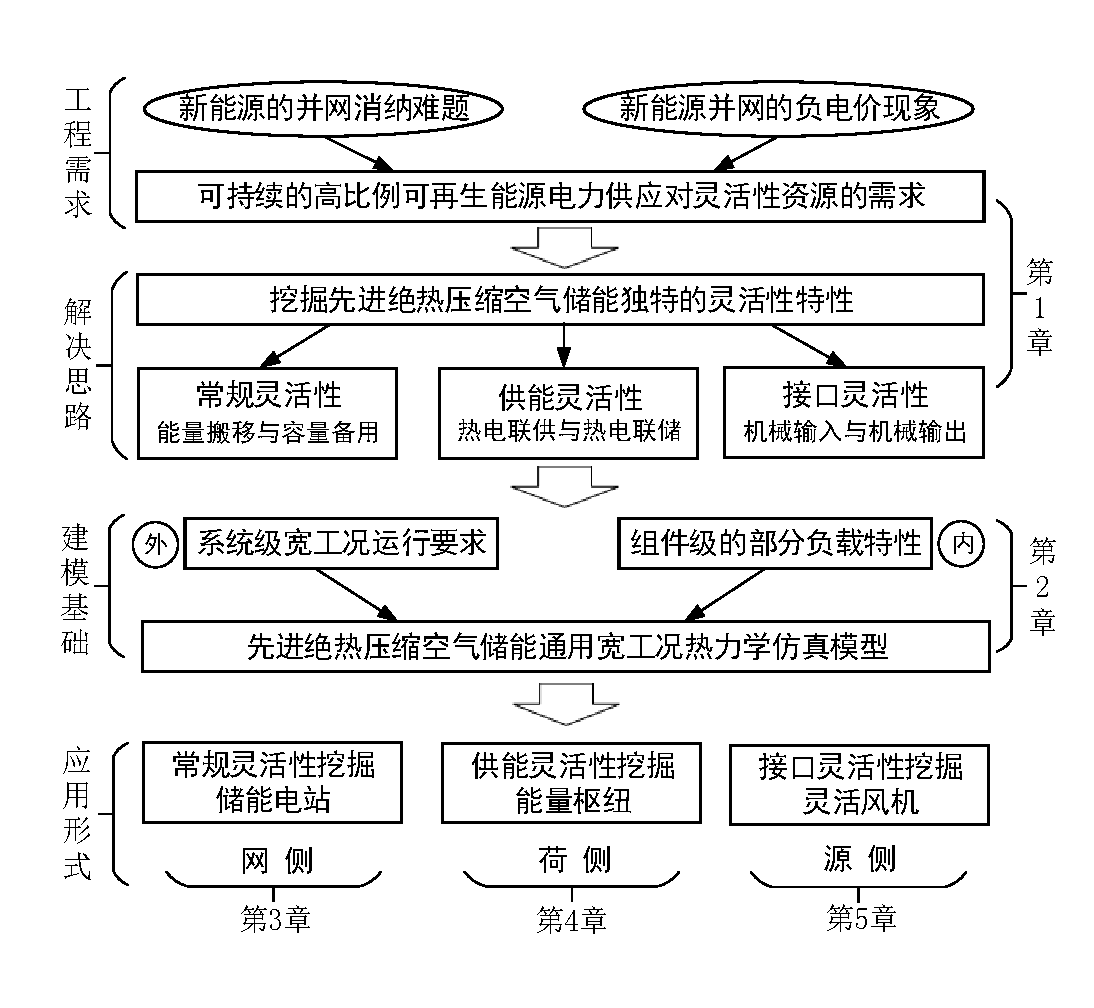
\includegraphics[scale=0.75]{figures/Chap1-4-Thesis-Framework-3.pdf}
  \caption{论文组织架构}
  \label{fig:Thesis-Framework}
\end{figure}

在\textbf{挖掘以能量搬移与容量备用为特征的常规灵活性}方面,研究了以高效储能(灵活储能)形式支撑电力系统运行的AA-CAES 储能电站,并系统地提出了计及宽工况运行特性的储能电站建模、运行及运营方法。具体地:1)基于热力学宽工况仿真模型,提出了刻画AA-CAES独特的内部压力势能与压缩热能双能流解耦存储与耦合释能特性的宽工况热力学特性曲线簇;2)基于热力学特性曲线簇,构建了面向AA-CAES储能电站常规灵活性应用的宽工况储气—储热双荷电状态(State-of-Charge, SOC)能量模型、能量与备用模型及其扩展模型;3)将双SOC 模型应用于风—储协同系统调度运行、日前电力市场策略竞标等问题,指导应用于电力系统的AA-CAES储能电站的建模、运行与运营。

在\textbf{挖掘以热电联供与热电联储为核心的供能灵活性}方面,研究了以能量枢纽(灵活负荷)形式支撑热电综合能源系统运行的AA-CAES型能量枢纽,并系统地提出了AA-CAES 型能量枢纽在热电综合能源系统的建模、运行及运营方法。具体地:1)设计了基于AA-CAES的两类热电联供能量枢纽,建立了表征其供能灵活性的热电联供模型;2)提出了集中式运营环境下含AA-CAES型能量枢纽的区域热电综合能源系统调度方法,并提出了基于㶲理论的热电综合能源系统数量—质量联合建模方法,为热电等多能流品位建模难题提供了新思路;3)提出了独立运营环境下面向热电综合能源市场的AA-CAES型能量枢纽的市场竞标策略,以实现能量枢纽的经济运行与运营。

在\textbf{挖掘以机械输入与机械输出为内涵的接口灵活性}方面,研究了以风-储集成系统(灵活电源)形式从源头平滑风电出力波动性的内嵌AA-CAES的可调度风机,并系统地提出了其建模、运行及运营等方法。具体地:1)设计了内嵌先进绝热压缩空气储能的灵活可调度风机,实现高风速时段叶片未利用风能的回收与低风速时段短缺风能的填补,从源头上降低了风速与风功率间的瞬时强耦合特性;2)提出了克服风速波动对内嵌AA-CAES运行效率影响的措施,建立了面向电力系统应用的灵活风机能量模型及双备用模型;3)在风机发电能力评估的基础上,提出了含灵活风机的电力系统调度运行及灵活风机市场竞标方法,以实现灵活风机的高效运行及运营。

本文通过分析面向新能源电力系统应用时AA-CAES内部组件的部分负载运行特性,建立了通用宽工况热力学仿真模型,从网侧高效储能电站、荷侧灵活能量枢纽、源侧灵活可调度风机三个角度系统研究了典型先进绝热压缩空气应用形式的设计建模、调度运行及市场运营等问题,为充分挖掘先进绝热压缩空气储能独特的储能循环的常规灵活性、供能灵活性及接口灵活性提供了较为系统的建模与分析方法,为实现可持续的高比例可再生能源电力供应提供了新的解决方案\footnote{尽管本文标题为源-网-荷先进绝热压缩空气储能灵活性建模及运行研究,但后续章节的实际组织则以网、荷、源的顺序开展,其主要原因在于:1)网侧储能电站利用的常规灵活性最直观,荷侧能量枢纽利用的供能灵活性也较易发现,而源侧风储集成系统利用的接口灵活性则不宜发觉,这也是我们在第\ref{sec:flexibility-intro}节先分析常规灵活性与供能灵活性,最后再分析接口灵活性的初衷;2)网侧储能电站、荷侧能量枢纽为电力系统注入的灵活性本质上是对新能源电力接入电力系统带来的不确定性及增加的灵活性资源需求的一种“被动补救”措施,而源侧风-储集成风机有望从源头上解决风电功率的波动性并降低对风电并网对系统灵活性资源的需求,可视为一种“主动预防”措施,按照“被动”-“主动”的逻辑组织结构更耐人寻味。}。总之,本文工作实现了一种“事后补救”与“提前预防”相结合的电力系统灵活性支撑方案,以网侧储能电站与荷侧能量枢纽“被动”满足当前电力系统的灵活性资源需求,提升现有电力系统对新能源的接纳能力;以源侧灵活风机在不增加(未来)风电的接入对系统灵活性资源的需求同时“主动”提供灵活性资源,从而满足未来电力系统对高比例新能源的并网消纳需求。


\chapter{先进绝热压缩空气储能通用宽工况热力学仿真模型}
\label{cha:simulation}

\section{概述}
\label{sec:chap2-intro}

电池储能作为电化学储能中的典型代表,存在着不同种类的变体,如铅酸电池、镍镉电池、锂电池等\cite{Battery-Nature-15, ESS-Review-09}。同样地,AA-CAES也存在多种实现形式,如本文关注的经典AA-CAES储能(第\ref{cha:aa-caes}章)、多能联供型AA-CAES(第\ref{cha:st-caes}章)、风-储集成型AA-CAES(第\ref{cha:ca-recs}章)等。类似于电池储能各变体的基本组件及特性大同小异,AA-CAES各实现形式均包含压缩机、空气透平、换热器、储气库、储热系统等基本组件,深入分析各基本组件的运行特性并建立相应的稳态热力学仿真模型是研究AA-CAES系统级运行特性及调度运行与市场运营方法的前提。

在新能源电力系统应用背景下,AA-CAES各实现形式均不同程度的运行于非额定工况。具体地,若应用于电源侧与风电协同,则压缩机与空气透平将处于部分负载运行;若应用于电网侧削峰填谷及容量备用,AA-CAES将响应价格与负荷波动运行非额定工况;若应用于多能互补系统,AA-CAES内部组件将通过运行于非设计工况响应电热负荷需求的频繁变化。因此,需要分析外部运行环境提出的宽工况运行要求引起的内部组件的部分负载运行特性对AA-CAES整体运行特性的影响。

实现准确的热力学特性建模是分析AA-CAES宽工况运行性能的基本前提。本章提出了计及组件部分负载运行特性的AA-CAES通用宽工况热力学仿真模型,考虑了“定压—定压”、“定压—滑压”、“滑压—定压”、“滑压—滑压”等四种不同的膨胀机与压缩机运行模式;针对容积控制型储气库,建立通用定容、等温、绝热三种储气库模型,进而构建了基于热力学第一定律与热力学第二定律的通用仿真模型,从而为后续章节应用于新能源电力系统源、网、荷侧的不同AA-CAES实现形式的建模与分析奠定基础。

本章结构安排如图~\ref{fig:Model-Flow-Chart}所示,第~\ref{sec:chap2-struc-supply}~节考虑包含各常规组件的典型AA-CAES系统结构,分析其运行模式与供能模式,为研究系统级宽工况热力学仿真模型提供依据;第~\ref{sec:part-load-energy}~ 节基于热力学第一定律,建立~AA-CAES~各组件的部分负载仿真模型及边界条件;第~\ref{sec:chap2-part-load-exergy}~节基于热力学第二定律,建立各组件的宽工况㶲模型;第~\ref{sec:chap2-bound-measure}~节基于构建的热力学仿真模型分析一典型 AA-CAES系统的内部热力学特性及外部供能特性。
%从而为第\ref{cha:aa-caes}章至第\ref{cha:ca-recs}章源—网— 荷三侧典型AA-CAES应用形式的准确建模与运行方法研究提供基础。

\begin{figure}[H] % use float package if you want it here
  \centering
  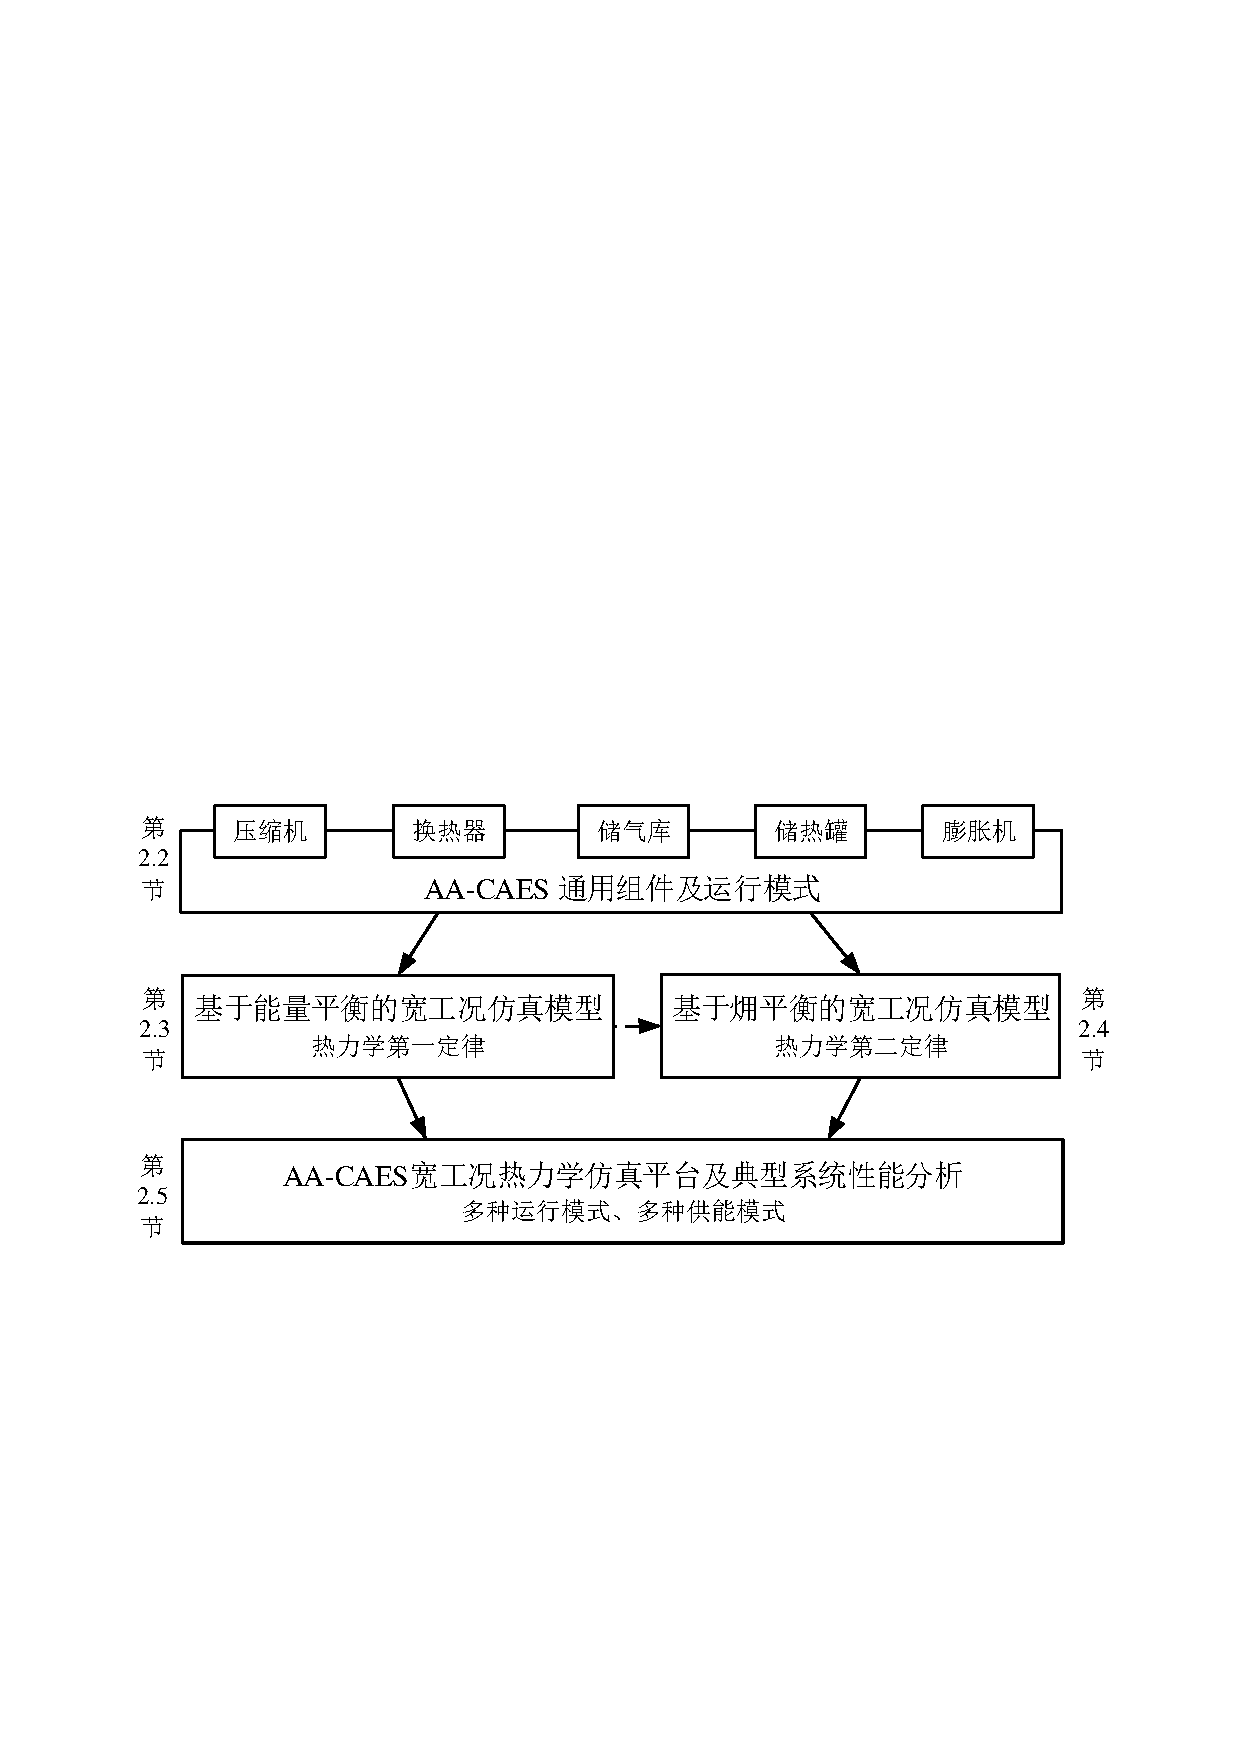
\includegraphics[scale=0.80]{figures/Chap2-1-Model-Flow-Chart-V6.pdf}
  \caption{第2章结构安排}
  \label{fig:Model-Flow-Chart}
\end{figure}

\section{运行模式与供能模式}
\label{sec:chap2-struc-supply}
\subsection{系统结构}
为实现较高的电效率及热利用率,AA-CAES一般采用“多级压缩、级间冷却”与“多级膨胀、级间再热”结构,以逼近“局部准绝热,整体准等温”\cite{Thesis-Zhangxuelin}的热力学流程,如图~\ref{fig:CAES-thermal-struc}所示的典型两级压缩、两级膨胀系统(图中LP与HP分别表示低压级与高压级)。为进一步提高系统的能量利用效率,实际电站(如McIntosh 电站)一般会采用透平乏气(排气)预热透平入口空气。本章重点关注内部组件级的部分负载热力学特性,不考虑采用透平乏气预热空气以提升透平入口空气焓值的做法。

\begin{figure}[H] % use float package if you want it here
  \centering
  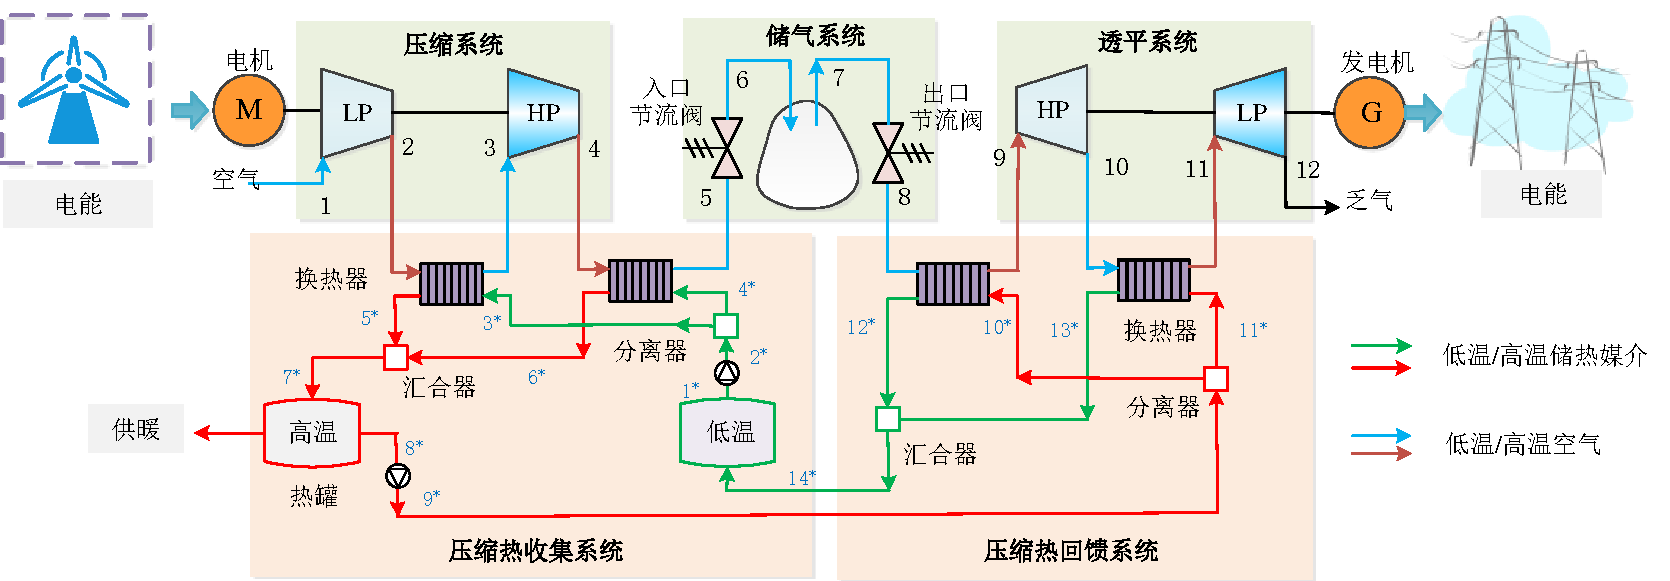
\includegraphics[scale=0.57]{figures/Chap2-1-AA-CAES-Struc-Thermo.pdf}
  \caption{典型AA-CAES结构示意图}
  \label{fig:CAES-thermal-struc}
\end{figure}

为便于分析,除特殊说明外,本章及后续章节AA-CAES各实现形式的热力学特性分析、建模及运行与运营等问题中采用如下假设:
\begin{itemize}
  \item 空气为理想气体, 满足理想气体状态方程;
  \item 空气与传热介质及储热介质的比热容均为常数\footnote{工程热力学中存在更精确的比热容计算方法,如采用首末热力学状态点的平均比热容等,本文不予考虑。};
  \item 不考虑压缩机与电动机、膨胀机与发电机间的能量转换效率(或能量损失);
  \item 忽略压缩热收集与回馈系统中储热介质及载热流体升压泵的耗功;
  \item 不计及载热介质经过泵后引起的温度变化;
  \item 储气库入口及出口的空气节流(若部署相应的节流阀)过程均为绝热过程;
  \item 仅考虑定容储气库模型, 不考虑定压储气库模型;
  \item 不考虑储气库的气体泄漏问题;
  \item 忽略整个过程中工作介质的动量变化及重力势能变化。
  \item 忽略相关管道的热耗散与压力损失。
\end{itemize}

\subsection{运行模式(压力视角)}
根据压缩机背压以及透平入口空气压力的恒定与否,CAES电站可以存在多种运行模式。针对D-CAES电站,文献\inlinecite{CAES-Discharge-16}研究了由储气库出口侧节流阀的控制实现的固定入口空气压力(定压)与变入口空气压力(滑压)等透平运行模式。针对AA-CAES型多能联供系统,文献\inlinecite{CAES-CCHP-off-design-18}引入了由储气库入口与出口节流阀的有无界定的四种运行模式。为实现更加通用的宽工况热力学特性建模,本文引入文献\inlinecite{CAES-Discharge-16,CAES-CCHP-off-design-18}中的运行模式概念。具体地,由末级压缩机出口空气压力与首级膨胀机入口空气压力是否(相对)恒定来界定如下四种运行模式:

(1)定压—定压

 定压—定压运行模式下,图~\ref{fig:CAES-thermal-struc}中入口侧及出口侧的节流阀均处于投入状态。储气库入口侧节流阀的入口空气压力为储气库的最大工作压力,背压为储气库实时压力;出口侧节流阀的入口压力为储气库实时压力,出口压力为储气库的最小工作压力。

(2)定压—滑压

 定压—滑压运行模式下,图~\ref{fig:CAES-thermal-struc}中入口侧节流阀处于投入状态,出口侧节流阀处于停滞状态。储气库入口侧节流阀的入口压力为储气库最大工作压力,背压为储气库实时压力;首级透平的入口空气压力为储气库实时压力,透平处于变压力运行方式。

(3)滑压—定压

滑压—定压运行模式下,图~\ref{fig:CAES-thermal-struc}中储气库入口侧节流阀处于停滞状态,出口侧的节流阀处于投运状态。末级压缩机的出口压力为储气库实时压力,处于变压力运行方式;出口侧节流阀的入口压力为储气库实时压力,出口压力为储气库最小工作压力。

(4)滑压—滑压

滑压—滑压运行模式下,储气库入口侧及出口侧节流阀均处于停滞状态。末级压缩机的出口空气压力与首级透平的进口空气压力均为储气库实时压力,压缩机与膨胀机均处于变压力运行模式。

需要说明的是,通过引入节流阀可以在一定程度上改善压缩机与膨胀机的运行工况,当然也会导致一定的节流损失。然而,上述四种运行模式中通过节流阀维持压缩机和膨胀机的出口与入口空气压力处于额定值的思路仅能改善压缩机和膨胀机受储气库空气压力变化而引起的偏离设计点运行的情形,难以消除AA-CAES因受外部宽工况运行指令导致的压缩机与膨胀机因质量流率等偏离设计点以及储气库中空气与储热系统中储热介质的温度变化等引起的部分负载状态下的低效运行问题。在一定条件下,该问题可通过压缩机与膨胀机的最优转速控制来改善,如文献\inlinecite{ST-CAES-Control-18-CXT}中针对光热复合压缩空气储能系统膨胀机的最优转速控制,以及文献\inlinecite{CA-RECS-Model-Rui-18} 中压缩/膨胀复合机的最优转速控制等。事实上,膨胀机受入口空气温度变化引起的部分负载运行可通过在膨胀机入口与换热器出口间增设电阻丝加热装置等(如文献
\inlinecite{HTH-CAES-Berk-18})进行抑制;本文不考虑该情形,但本文后续的分析方法仅做适当修改即可适用于该类系统。

\subsection{供能模式(温度视角)}
为便于后续章节研究以储能形式应用的AA-CAES电站、以负荷形式应用的AA-CAES能量枢纽,本文假设AA-CAES具有供电模式与热电联供模式等两种供能模式。由于发电机(电动机)电能-机械能(机械能-电能)的转换效率很高,源侧利用AA-CAES的机械输入与输出接口的过程中去除(压缩机前的)电动机与(膨胀机后的)发电机时的供能模式可视为供电模式的特例。

(1)供电模式

 在供电模式下,AA-CAES透平侧需要的入口空气温度较高,往往需反馈全部压缩热,或同时辅助末级透平乏气预热首级透平进口温度。此时,压缩阶段收集的压缩热可富余的供热量较少,AA-CAES 主要应用于电力系统电能单能流应用场景。该模式是面向电力系统的AA-CAES储能电站的主要供能模式,在该模式下AA-CAES储能电站可参与电量市场及辅助服务市场进行运营。

(2)热电联供模式

在热电联供模式下,压缩阶段收集的压缩热能可部分用于供热,存在压缩-供热、静置-供热及膨胀-供热等情形。此时,回馈给透平发电阶段的压缩热较少,透平的入口空气温度较低,从而导致透平排气温度较低,具备制冷能力。该模式主要应用于面向分布式多能互补系统或区域综合能源系统中的AA-CAES型能量枢纽。正如第
\ref{sec:flexibility-poly-generation}节分析,在热电联供模式下一般需要辅助其它(外部)热源,以提高能量枢纽的热电联供能力。

%\subsection{热力学特性与系统效率}
%分析AA-CAES内部组件的功–能转换特性与动态特性,揭示空气压缩热能与空气压力势能间的能流耦合机理,探寻能效提升措施,进而设计面向源-网-荷侧不同应用场景的结构形式,是充分挖掘可再生能源系统中AA-CAES的常规灵活性、供能灵活性及接口灵活性的前提。效率是AA-CAES应用研究中最为关心的问题之一,是制约CAES技术推广应用的瓶颈。一般而言,AA-CAES的效率可从额定工况点效率与宽工况运行效率两个方面进行考察\cite{CAES-Review-18-Rui-operation}。

%\subsubsection{额定工况效率}
%与电池储能、抽水蓄能等技术的循环效率评估方式不同,AA-CAES 效率评估具有其独特的多能流输入及多能流输出特性,具体表现在因富余压缩热能、透平乏气或外部光热热源供热赋予的热能、电能联供能力,使得AA-CAES具备了多能流(输入)输出特性。为此,本文重点关注AA-CAES在仅供电模式下的电–电转换效率与多能联供模式下的能量综合利用效率。其中,电–电转换效率表征一个循环周期内透平发电机产生的电能与压缩机消耗的电能之比;能量综合利用效率则充分计及AA-CAES 所能提供的多能流产品,表征多能流产品总能量(包括储热系统存储的压缩热能、发电机输出的电能及透平低温排气冷能)与压缩环节消耗的电能之比~\cite{CAES-Review-16-Xue-EI}。

%AA-CAES额定工况点的效率一般在设计阶段从内部的组件结构及参数配置等层面~\cite{A-CAES-Therm-12,RCAES-Para-14,AA-CAES-Eff-Struc-13} 予以保障,可概括为以下三个层次: 1)通过基于热力学仿真的压缩-透平级数结构配置方案实现具有较高效率的AA-CAES流程及结构\cite{AA-CAES-Eff-Struc-13,Ene-Exe-ACAES-17,Thesis-Zhangxinjin}; 2)在确定的AA-CAES 结构配置下,通过优化的温度、压比分配策略使得压缩机与空气透平性能接近设计点~\cite{Eff-Pow-MotCom-11,ACAES-Conf-12}; 3)在给定温度及压比分配策略下, 采用压缩/透平机械的最佳压缩/膨胀方式来克服压缩或膨胀过程中的非稳态区等~\cite{Eff-Pow-MotCom-11,WT-CAES-Market-15}。本文假定AA-CAES的结构配置与参数优化均已完成,重点研究其建模及运行等问题,特别是在不同运行模式下AA-CAES的运行特性。

%图~\ref{fig:Eff-Stage-No} 给出了不同配置方案对AA-CAES电– 电转换效率影响示意图,其中$\eta$为多变效率~\cite{A-CAES-Therm-12}。

%\begin{figure}[H] % use float package if you want it here
%  \centering
%  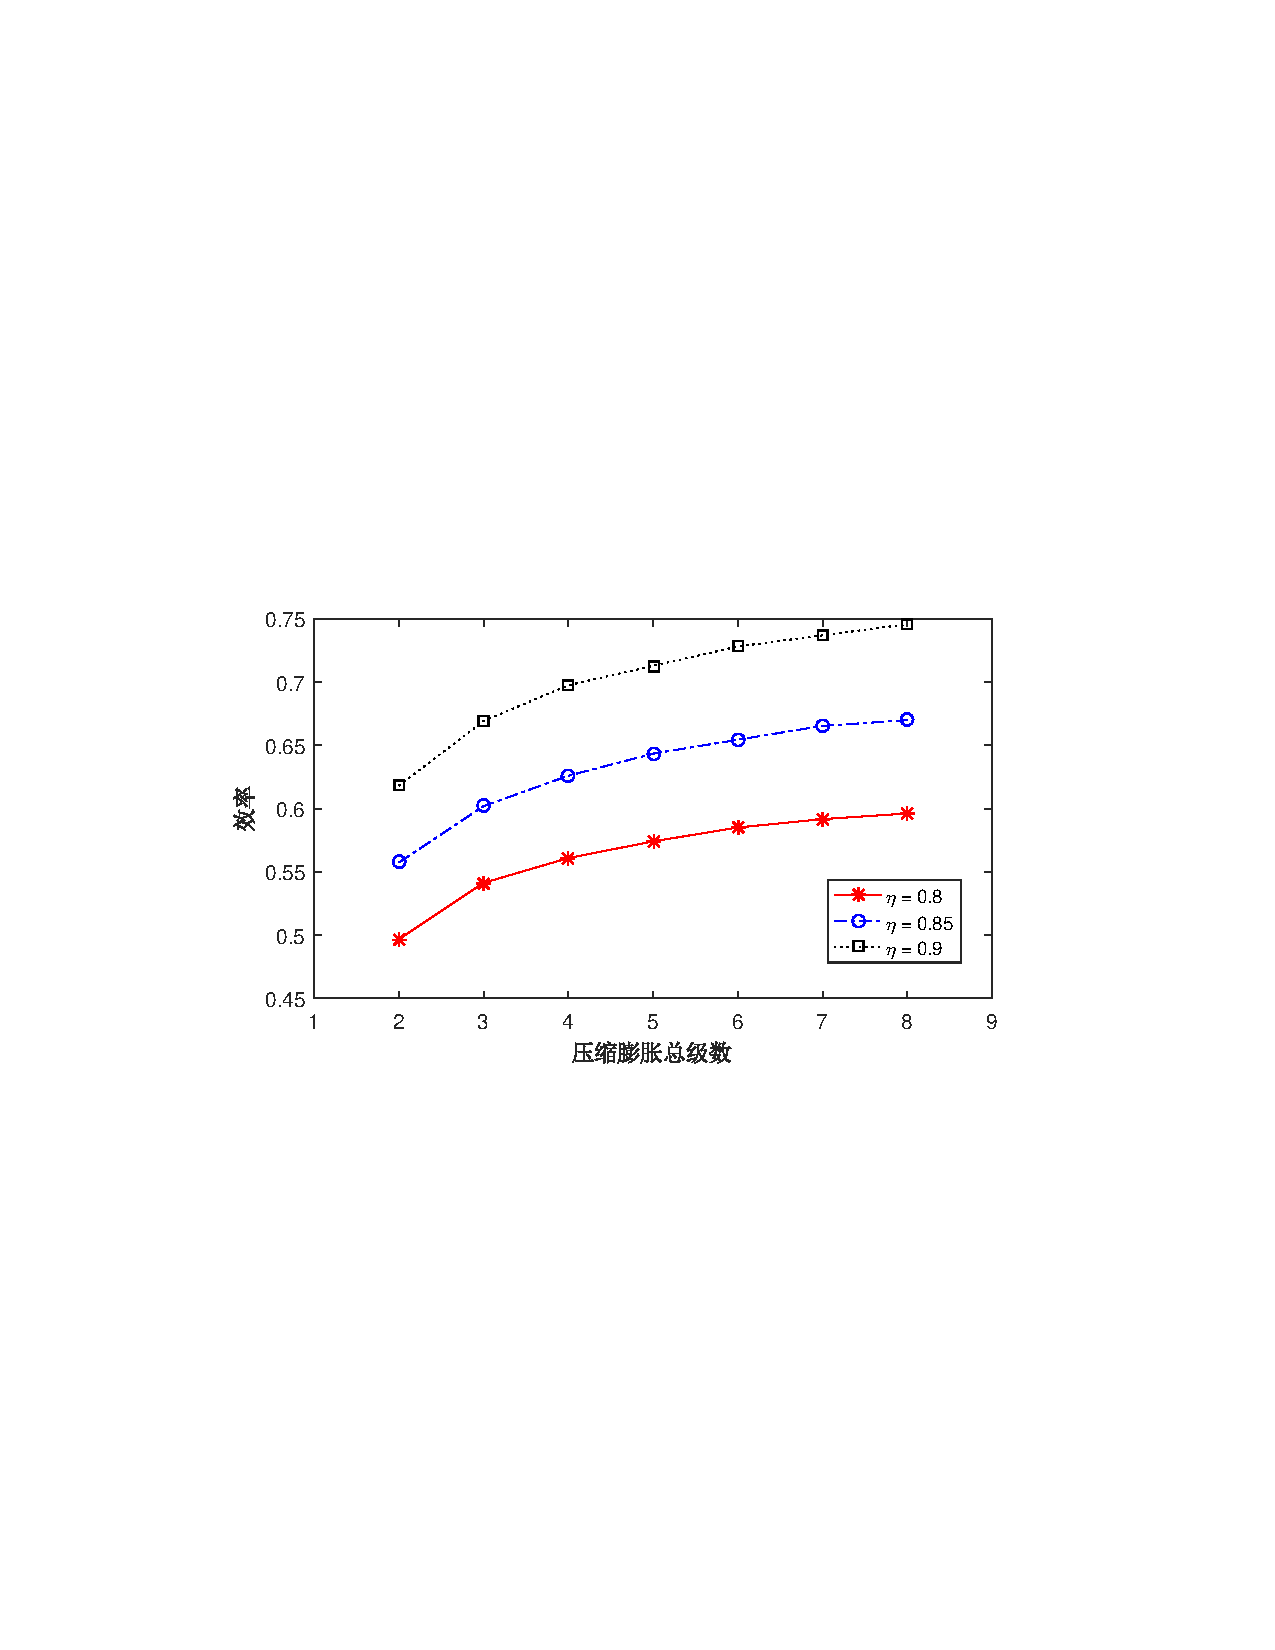
\includegraphics[scale=0.70]{figures/Chap1-6-Eff-Stage-No.pdf}
%  \caption{结构配置对电–电转换效率影响示意图}
%  \label{fig:Eff-Stage-No}
%\end{figure}

%在组件结构配置及参数优化方面,文献~\inlinecite{AA-CAES-Eff-Struc-13} 开展了压缩膨胀级数配置研究,通过仿真比较多种AA-CAES系统模型的功效率和㶲损失,给出了压缩机与透平膨胀机级数的最优组合。文献~\inlinecite{Ene-Exe-ACAES-17} 开展了AA-CAES系统的能量分析与㶲分析,指出最大㶲损出现在压缩机和透平,所设计的AA-CAES 系统电– 电转换效率达50\%,并指出通过增加压缩、膨胀级数和换热器可进一步减小㶲损,提高电–电转换效率。文献~\inlinecite{Thesis-Zhangxinjin} 系统分析了压缩膨胀级数组合对D-CAES及AA-CAES功效率及㶲效率的影响机制。文献~\inlinecite{Eff-Pow-MotCom-11} 关注系统运行过程中温度、压比及流量等参数对AA-CAES 效率的影响。但需说明的是,上述研究主要基于仿真方法配置AA-CAES结构,缺乏成熟优化方法指导设计,同时也很少考虑AA-CAES电站宽工况运行时工作点偏离设计点对结构配置及参数优化的影响机理。此外,在给定结构配置下温度及压比分配策略,以及宽工况运行条件下最优压缩发电运行的实现方式方面的探讨尚不充分。

%\subsubsection{宽工况运行效率}
%尽管通过组件结构及参数配置可在一定程度上确保AA-CAES在额定运行工况下达到较高的效率,但电力系统和综合能源系统对AA-CAES提出的宽工况运行要求\cite{EH-Form-14,IES-Disp-17} 将使其内部各组件频繁运行于非额定工况点,进而影响其电–电转换效率及综合能源利用效率。特别是在AA-CAES电站参与辅助服务时该问题将更加突出,在实际中需结合AA-CAES在一个周期内的整体运行工况分析其宽工况运行效率。

%具体而言,作为空气压力势能和压缩热能的解耦生产单元和耦合释能单元,压缩机和膨胀机(空气透平)在部分负载工况(非额定压缩和发电负荷)运行时效率变化明显。例如,压缩机、透平机械在额定设计点运行效率一般可达87\%-90\%,而50\%压缩/发电负荷时效率降至65\%-70\%,30\%压缩/发电负荷时效率甚至不及50\%~\cite{Eff-Pow-MotCom-11,CAES-Discharge-16}。 同时,作为空气压缩热能传输收集和传输释放单元的换热器亦存在部分负载运行特性,其换热系数易受热流流速(相应于压缩/发电负荷率)影响较大~\cite{HeatExch-Char-84,HE-Eff-CN-17}。

%文献~\inlinecite{CAES-PH-Char-11}分析了透平、膨胀机等组件运行特性对CAES系统效率的影响。文献~\inlinecite{ACAES-Conf-12} 建立了AA-CAES热力学模型,分析了温度、压比、工质流率等参数对其电-电转换效率的灵敏度。文献~\inlinecite{A-CAES-Therm-12,CAES-TES-Thermo-08} 分析了多级AA-CAES的热力学特性,强调了优化换热器的重要性。进一步,文献~\inlinecite{TES-Eff-CAES-13} 分析了蓄热系统对AA-CAES热力学特性的影响机制,定量评估了温度和压力对压缩热利用的影响效果。文献~\inlinecite{A-CAES-Dynamic-17} 计及内部压缩机与透平等组件的部分负载运行特性,建立了从组件性能到AA-CAES系统整体效率评估的仿真方法。

%综上,上述文献重点从热力学角度分析额定工况下AA-CAES系统运行参数对电-电转换效率或综合能效等的影响,较少探讨宽工况运行时AA-CAES系统的热力学特性及组件功-能转换机理,同时也较少关注非额定运行工况下压缩热能产生率、压缩热能损耗率、换热器传热特性及蓄热系统对储气库单位工质做功能力的提升机制等实际运行问题。本章第
%\ref{sec:part-load-energy}节与第\ref{sec:chap2-part-load-exergy}节将详细分析内部组件的部分负载特性与动态特性,进而分析AA-CAES系统级的宽工况运行特性,为揭示AA-CAES系统单位压缩功率压缩热能与压力势能产生量、单位发电功率压缩热能与压力势能消耗量、压缩与发电环节不同配比压缩热能与压力势能对压缩机耗功及透平出力的影响机理、压缩发电环节单位工质换热量与压缩发电功率水平的定量关系等奠定基础。

\section{基于热平衡的宽工况热力学仿真模型}
\label{sec:part-load-energy}
AA-CAES在削峰填谷、旋转备用、无功支撑、多能联供等典型场景的应用,要求其具有宽工况运行能力(20\%-110\%压缩功率/膨胀功率运行)。在宽工况运行条件下,压缩机、膨胀机等能量转换组件的运行特性(如效率等)变化明显。同时,换热器等能量转移组件的传热系数受到热工质流率的影响,不同质量流率下传热系数变化明显
\cite{HeatExch-Char-84,HE-Eff-CN-17},影响压缩热能的收集和回馈,进而改变AA-CAES系统的电-电转换性能与热电联供性能。文献\inlinecite{A-CAES-Dynamic-17}针对采用高温储热技术收集空气压缩热能的典型两级压缩两级膨胀系统的分析表明,当储热效率\footnote{此处的储热效率仅针对填充床储热型AA-CAES,不能适用于双罐储热型AA-CAES,其定义为一个循环周期内流出与流入填充床储热系统的空气焓值之比。}达到90\% 以上时,额定工况运行时AA-CAES 电-电效率可达74\%,当宽工况运行时,其效率降为64\%。因此,当前采用的根植于电池储能的固定效率模型难以计及压缩机、膨胀机、换热器等组件的部分负载运行特性对AA-CAES 整体性能的影响。本节基于热力学第一定律建立能量转换组件与能量转移组件的部分负载热力学模型,以及能量存储组件的热力学动态模型,最后给出AA-CAES系统级的宽工况热力学仿真模型。

\subsection{能量转换类模块}

对AA-CAES各应用形式而言,一般均包含压缩机、空气透平等能量转换类组件,本小节分别给出二者在额定工况以及部分负载工况下的稳态热力学模型。

\subsubsection{压缩机}
\label{sec:part-load-energy-compressor}
%\subsubsection{部分负载特性概述}

\textbf{(1)额定工况能量平衡关系}

%第$i$级压缩机等熵压缩出口温度满足,
%\begin{equation}
%\label{equ:comp-iso-temp}
%T_{c,i}^{out,is} = T_{c,i}^{in}{\left( {{\beta _{c,i}}} \right)^{\frac{{k - 1}}{k}}}
%\end{equation}
%其中,$T_{c,i}^{in}$ 为压缩机入口空气温度,$k$ 为空气绝热指数,取值为1.4。

第$i$级压缩机出口空气温度可由等熵效率计算\cite{Eng-Thermo-83},即
% \begin{equation}
%\label{equ:comp-real-temp-1}
%{\eta _{c,i}} = \frac{{T_{c,i}^{out,is} - T_{c,i}^{in}}}{{T_{c,i}^{out} - T_{c,i}^{in}}}
%\end{equation}
%即,第$i$级压缩机实际出口空气温度为
 \begin{equation}
\label{equ:comp-real-temp-2}
T_{c,i}^{out} = \frac{1}{{{\eta _{c,i}}}}T_{c,i}^{in}({{{({{\beta _{c,i}}})}^{\frac{{k - 1}}{k}}} + {\eta _{c,i}} - 1})
\end{equation}
其中,$\eta _{c,i}$ 为压缩机等熵效率;$T_{c,i}^{in}$ 为压缩机入口空气温度;$k$ 为空气绝热指数,取值为1.4\footnote{更精确的计算可采用多变指数代替绝热指数$k$, 本文不予考虑。};${\beta _{c,i}}$ 为压缩机压比。

第$i$级压缩机实际耗功(功率)及所有压缩机总耗功分别为
\begin{subequations}
\begin{gather}
{W_{c,i}} = {\dot m_c}c_p^a({T_{c,i}^{out} - T_{c,i}^{in}})\label{equ:comp-power}\\
{W_c} = \sum\limits_{i = 1}^{{N_c}} {} {W_{c,i}} \label{equ:comp-power-total}
\end{gather}
\end{subequations}
其中, $\dot m_c$为压缩机空气质量流率;$N_c$ 为压缩机级数;$c_p^a$ 为空气的定压比热容\footnote{若需进行更精确的仿真,可采用焓值计算耗功
\cite{Eng-Thermo-83},即${W_{c,i}} = {\dot m_c}({h_{c,i}^{out} - h_{c,i}^{in}})$。}。

第$i$级压缩机出口空气压力为
\begin{equation}
\label{equ:comp-pressure}
p_{c,i}^{out} = p_{c,i}^{in}{\beta _{c,i}}
\end{equation}
其中,$p_{c,i}^{in}$ 为进口空气压力; $p_{c,i}^{out}$为出口空气压力。

后文研究中不计及压缩机的部分负载运行特性时,即可采用额定工况稳态热力学模型(\ref{equ:comp-real-temp-2})-(\ref{equ:comp-pressure})。

\textbf{(2)部分负载特性解析模型}

作为空气压力势能和压缩热能的解耦生产单元,压缩机的压比$\beta _{c,i}$与等熵效率$\eta _{c,i}$ 随其运行工况变化。在额定设计点,压缩机的等熵效率一般可达87\%-90\%,而50\% 压缩负载时其等熵效率降至65\%-70\%,30\%压缩负载时等熵效率甚至不及50\% ~\cite{CAES-Review-18-Rui-operation}。文献
\inlinecite{A-CAES-Therm-12}指出采用变效率方程(二次曲线)来刻画压缩机的部分负载运行特性,即
\begin{equation}
\label{equ:comp-eff-quad}
{\eta _{c,i}} = {({{\eta _{c,i}}})_0} - {\alpha _c}{({{{({{\beta _{c,i}}})}_0} - {\beta _{c,i}}})^2}
\end{equation}
其中,${\alpha _c}$ 为常数;${(\cdot)_0}$ 表示设计工况下的参数,后文相同。但该方法仅能给出等熵效率随压比变化的近似关系,难以揭示压缩机部分负载运行时非额定质量流率引起压比及等熵效率变化的物理本质。文献\inlinecite{Compressor-thermo-02}给出了部分负载运行工况下单轴燃气轮机中压缩机及透平的特性曲线的解析表达式,为仿真压缩机的部分负载运行特性提供了依据。文献\inlinecite{Compressor-Review-17}给出了压缩机特性参数的典型回归方法,可用于燃气轮机热力学仿真模型的构建。鉴于文献\inlinecite{Compressor-thermo-02}中的部分负载解析方法在填充床储热型AA-CAES的热力学特性分析\cite{A-CAES-Dynamic-17}、 低温储热型AA-CAES的㶲特性分析~\cite{CHS-CAES-off-19}、AA-CAES 型CCHP系统\cite{AA-CAES-Simulation-19}及其它诸多热力系统仿真中得到较多应用,本节引入文献\inlinecite{Compressor-thermo-02} 中的压缩机特性图的解析表达式来描述其部分负载特性。

部分负载运行时压缩机的实际压比及实际等熵效率可分别表示为\cite{Compressor-thermo-02,A-CAES-Dynamic-17}
\begin{subequations}
\label{eq:com-iso-eff-off}
\begin{gather}
\frac{{{\beta _{c,i}}}}{{{{({{\beta _{c,i}}})}_0}}} = {a_{1,i}}{({{{\dot G}_{c,i}}})^2} + {a_{2,i}}{\dot G_{c,i}} + {a_{3,i}}\label{equ:comp-press-part}\\
\frac{{{\eta _{c,i}}}}{{{{({{\eta _{c,i}}})}_0}}} = [{1 - c{{({1 - {{\dot n}_{c,i}}})}^2}}]({{{\dot n}_{c,i}}/{{\dot G}_{c,i}}})({2 -({{{\dot n}_{c,i}}/{{\dot G}_{c,i}}})})\label{equ:comp-eff-part}
\end{gather}
\end{subequations}
其中,($a_{1,i}$, $a_{2,i}$, $a_{3,i}$)为表征转速对压比影响的因子;${\dot G_{c,i}}$ 与 ${\dot n_{c,i}}$ 分别为无量纲降阶流率与降阶转速,满足:
\begin{subequations}
\label{eq:com-mass-off}
\begin{gather}
{\dot G_{c,i}} = [{{{\dot m}_c}\frac{{{{({T_{c,i}^{in}})}^{0.5}}}}{{p_{c,i}^{in}}}}]/{[{{{\dot m}_c}\frac{{{{({T_{c,i}^{in}})}^{0.5}}}}{{p_{c,i}^{in}}}}]_0}\label{equ:reduced-comp-mass-flow}\\
{\dot n_{c,i}} = [{{n_c}{{({T_{c,i}^{in}})}^{-0.5}}}]/{[{{n_c}{{({T_{c,i}^{in}})}^{-0.5}}}]_0}\label{equ:reduced-comp-speed}
\end{gather}
\end{subequations}
其中,$n_c$为压缩机转速,对于采用变频调速等方式调节各级压缩机转速的实际系统,可修正(\ref{equ:reduced-comp-speed})中的$n_c$为$n_{c,i}$。定义中间变量
\begin{equation}
\label{equ:comp-mid-var-1}
{a_{0,i}} = [{{b_1}({1 - \frac{{{b_2}}}{{{{\dot n}_{c,i}}}}}) + {{\dot n}_{c,i}}{{({{{\dot n}_{c,i}} - {b_2}})}^2}}]
\end{equation}
则其它时变系数参数满足:
\begin{equation}
\label{equ:comp-mid-var-2}
{a_{1,i}} = \frac{{{{\dot n}_{c,i}}}}{{{a_{0,i}}}}, {a_{2,i}} = \frac{{({{b_1} - 2{b_2}\dot n_{c,i}^2})}}{{{a_{0,i}}}}, {a_{3,i}} = \frac{{{b_2}^2\dot n_{c,i}^3 - {b_1}{b_2}{{\dot n}_{c,i}}}}{{{a_{0,i}}}}
\end{equation}
其中,($b_1$, $b_2$, $c$) 为常系数,其典型取值为(1.8, 1.4, 0.3)~\cite{Compressor-thermo-02}, (0.36, 1.06, 0.3)~\cite{A-CAES-Dynamic-17}, (1.8, 0.93,0.3)~\cite{AA-CAES-Simulation-19}或(1.7, 0.93, 0.4)~\cite{AA-CAES-Simulation-19},对实际给定的压缩机可由其特性图进行拟合
\cite{Compressor-Off-Design-05},但需满足$b_1^{1/3}\le 2b_2/3$。

基于部分负载解析模型(\ref{eq:com-iso-eff-off})-(\ref{equ:comp-mid-var-2})可得如图~\ref{fig:Comp-Ratio-off-design}~ 及图~\ref{fig:Eff-part-load}~所示的压缩机压比及等熵效率的典型曲线\cite{CAES-Wind-Rui-19}。如此,基于部分负载工况下的实际压比及实际等熵效率,在给定实际入口温度及实际入口压力的条件下即可获得第$i$ 级压缩机的实际耗功、实际出口温度、实际出口压力。

\begin{figure}[H] % use float package if you want it here
  \centering
  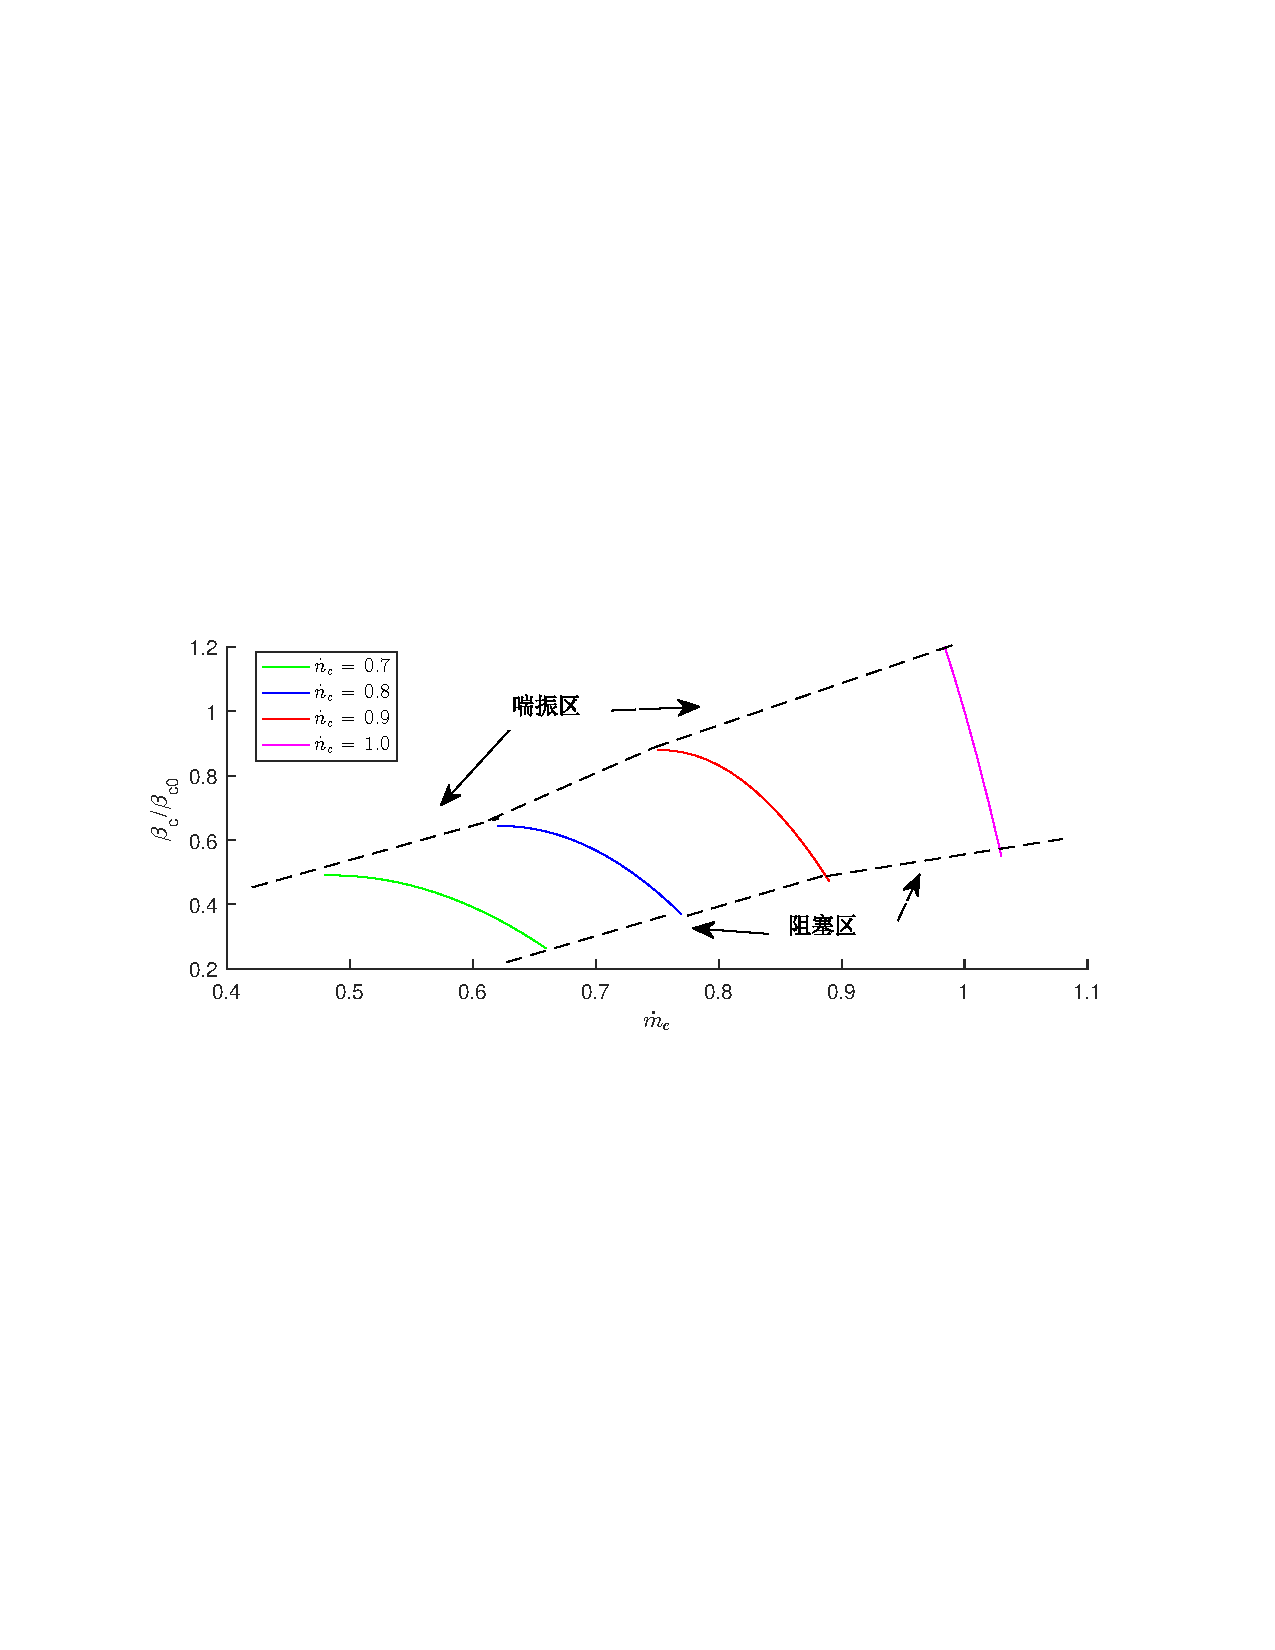
\includegraphics[scale=0.70]{figures/Chap2-2-Comp-Ratio-off-design.pdf}
  \caption{基于解析模型的压缩机部分负载压比}
  \label{fig:Comp-Ratio-off-design}
\end{figure}

\begin{figure}[H] % use float package if you want it here
  \centering
  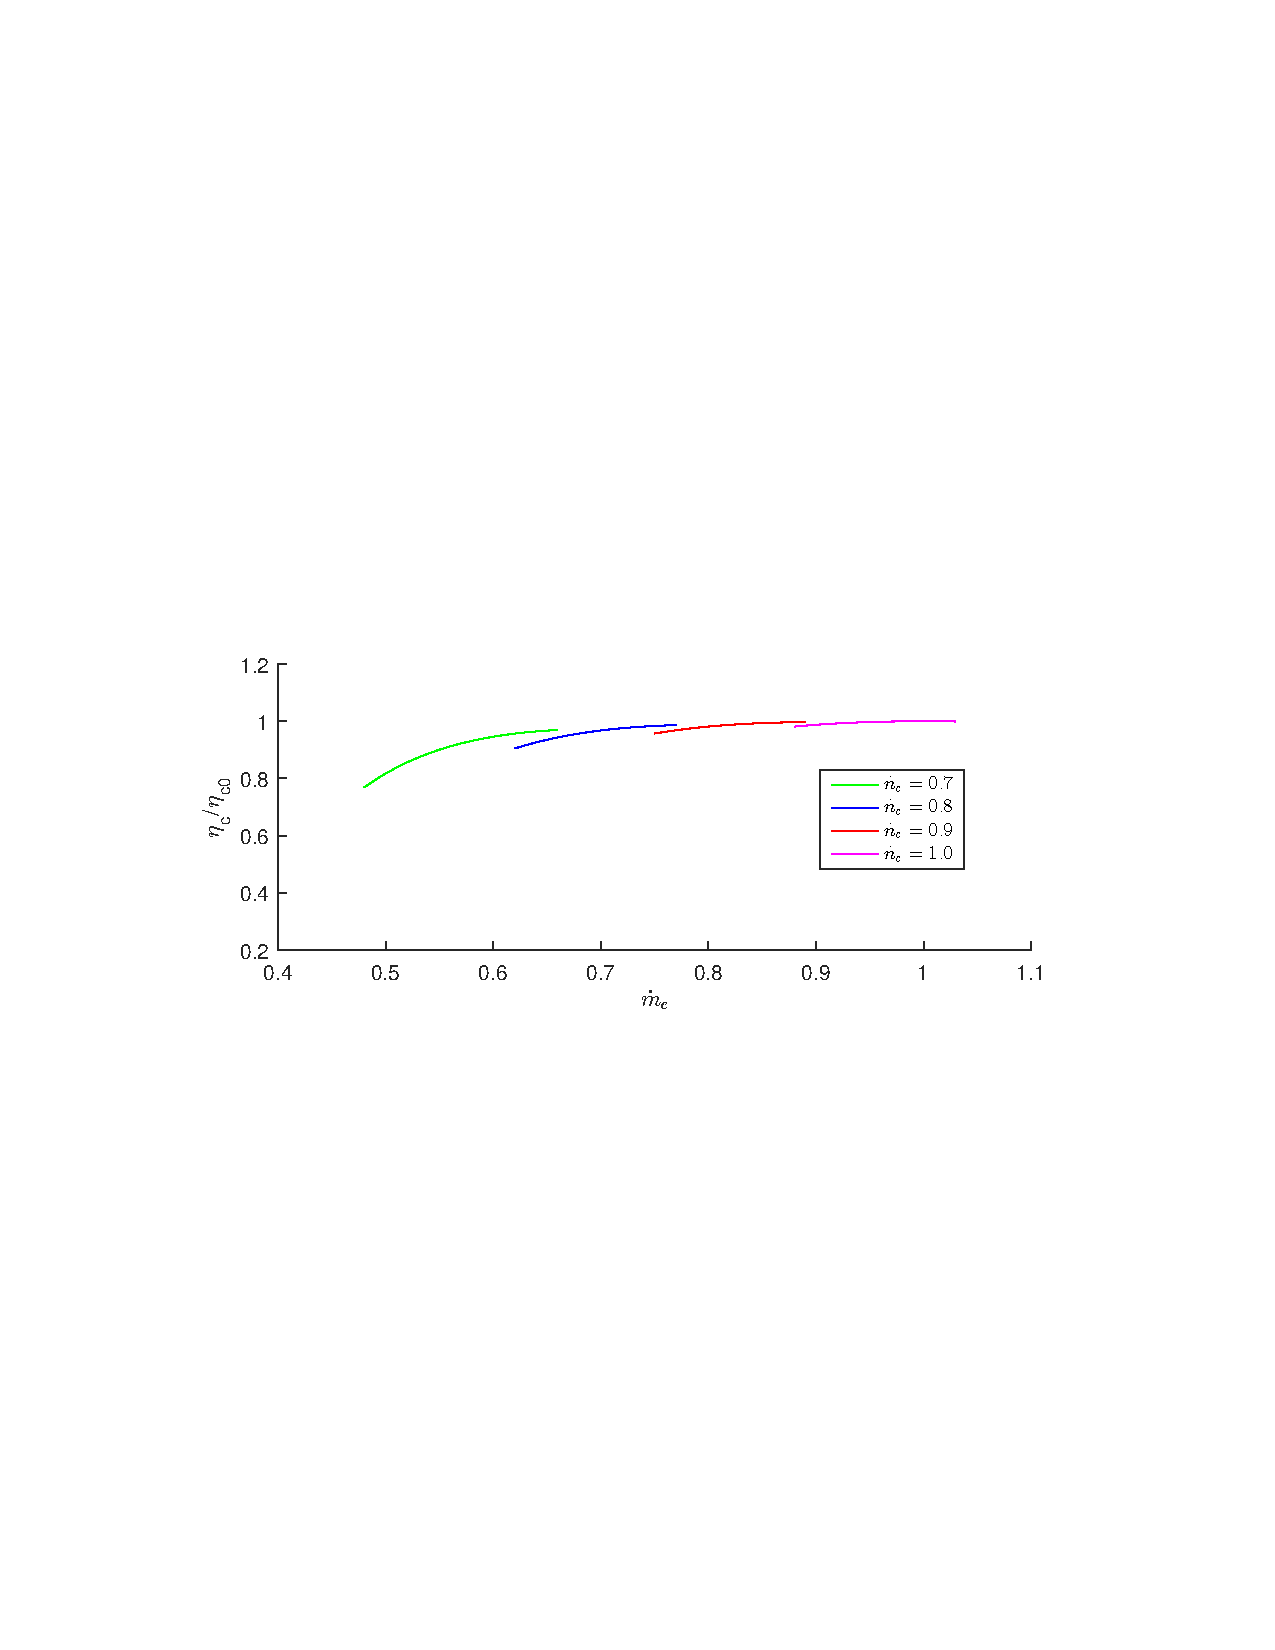
\includegraphics[scale=0.80]{figures/Chap2-3-Eff-part-load.pdf}
  \caption{基于解析模型的压缩机部分负载等熵效率}
  \label{fig:Eff-part-load}
\end{figure}

压缩机额定工况热力学模型(\ref{equ:comp-real-temp-2})-(\ref{equ:comp-pressure})及部分负载热力学模型(\ref{equ:comp-real-temp-2})-(\ref{equ:comp-mid-var-2}) 中的变量如表~\ref{tab:comp-thermo-para}~所示。在实际运行中的任一给定时刻,第1级压缩机入口温度$T_{c,1}^{in}$及入口压力$p_{c,1}^{in}$ 为确定值,外界电网调度指令会给出实时功率$W_c$,其它边界条件可通过后续组件确定。

\begin{table}[htb]
  \centering
  \begin{minipage}[t]{0.9\linewidth} % 如果想在表格中使用脚注,minipage是个不错的办法
  \caption{压缩机部分负载热力学模型变量表}
  \label{tab:comp-thermo-para}
    \begin{tabularx}{\linewidth}{cccccc}
      \toprule[1.5pt]
      {\heiti 变量} & {\heiti 物理意义} & {\heiti 单位} &  {\heiti 变量} & {\heiti 物理意义} & {\heiti 单位} \\\midrule[1pt]
      ${W_{c,i}}$ & 耗(电)功 & kW  &  ${\dot m_c}$ & 空气质量流率 & kg/s \\
      ${\beta _{c,i}}$ & 实际压比 & —— &  ${\eta _{c,i}}$ & 等熵效率 & —— \\
      $p_{c,i}^{in}$ & 空气进口压力 & kPa & $p_{c,i}^{out}$ & 空气出口压力 & kPa \\
      $T_{c,i}^{in}$ & 空气进口温度 & K & $T_{c,i}^{out}$ & 空气出口温度 & K \\
      ${n_{c,i}}$ & 实际转速 & r/min & $\dot n_{c,i}$ & 无量纲降阶转速 & —— \\
      $a_{0,i}$, $a_{1,i}$ & 中间变量 & —— & $a_{2,i}$, $a_{3,i}$ & 中间变量 & ——\\
      ${\dot G_{c,i}}$ &  无量纲降阶质量流率 &  —— & & &\\
      \bottomrule[1.5pt]
    \end{tabularx}
  \end{minipage}
\end{table}

\subsubsection{空气透平}
\label{sec:part-load-energy-turbine}


\textbf{(1)额定工况能量平衡关系}

%第$i$级膨胀机等熵膨胀出口温度满足,
%\begin{equation}
%\label{equ:turb-iso-temp}
%T_{e,i}^{out,is} = T_{e,i}^{in}/{\left( {{\beta _{e,i}}} \right)^{\frac{{k - 1}}{k}}}
%\end{equation}

第$i$级膨胀机出口空气温度可由等熵效率计算\cite{Eng-Thermo-83},即
% \begin{equation}
%\label{equ:turb-real-temp-1}
%{\eta _{c,i}} = \frac{{T_{c,i}^{out,is} - T_{c,i}^{in}}}{{T_{c,i}^{out} - T_{c,i}^{in}}}
%\end{equation}
%
%第$i$级膨胀机实际出口温度为,
 \begin{equation}
\label{equ:turb-real-temp-2}
T_{e,i}^{out} = T_{e,i}^{in}({1 - {\eta _{e,i}} + {\eta _{e,i}}{{({{\beta _{e,i}}})}^{\frac{{1 - k}}{k}}}})
\end{equation}
其中,$\eta _{e,i}$为透平等熵效率;$T_{e,i}^{in}$ 为透平入口空气温度;$\beta _{e,i}$ 为透平膨胀比。

第$i$级膨胀机实际做功及所有膨胀机做的总功为
\begin{subequations}
\label{equ:turb-power-all}
\begin{gather}
{W_{e,i}} = {\dot m_e}c_p^a({T_{e,i}^{in} - T_{e,i}^{out}})\label{equ:turb-power}\\
{W_e} = \sum\limits_{i = 1}^{{N_e}} {{W_{e,i}}}\label{equ:turb-power-total}
\end{gather}
\end{subequations}
其中,$\dot m_e$为膨胀机空气质量流率;$N_e$ 为透平级数。

第$i$级膨胀机实际出口空气压力为
\begin{equation}
\label{equ:turb-pressure}
p_{e,i}^{out} = p_{e,i}^{in}/{\beta _{e,i}}
\end{equation}
其中,$p_{e,i}^{in}$ 为进口空气压力;$p_{e,i}^{out}$为出口空气压力。

与压缩机类似,后文研究中不计及空气透平的部分负载特性时,即可采用额定工况稳态热力学模型(\ref{equ:turb-real-temp-2})-(\ref{equ:turb-pressure})。

\textbf{(2)部分负载特性解析模型}

空气透平也存在类似于压缩机的部分负载运行特性,其等熵效率会随着运行工况发生大幅变化。在额定工况下透平的等熵效率可达85\%-90\%,而在50\%负载工况下等熵效率降至65\%-75\%\cite{CAES-Review-18-Rui-operation,CAES-Discharge-16}。 在膨胀释能过程中,随着储气压力的降低,储气室出口空气温度和压力均会变化~\footnote{一般认为,存在出口侧节流阀时仅入口温度会变化,不存在节流阀时入口温度与入口压力均会变化。},从而引起透平的部分负载工况运行。为刻画等熵效率随部分负载运行工况(通常由质量流率及转速偏离额定工况引起)的变化特性,引入膨胀机的部分负载特性解析表达式。实际部分负载运行时等熵效率特性满足\cite{Compressor-thermo-02, AA-CAES-Simulation-19}:
\begin{equation}
\label{equ:turb-eff-part}
{\eta _{e,i}}/{({{\eta _{e,i}}})_0} = [{1 - {b_0}{{({1 - {{\dot n}_{e,i}}})}^2}}]({{{\dot n}_{e,i}}/{{\dot G}_{e,i}}})({2 -({{{\dot n}_{e,i}}/{{\dot G}_{e,i}}})})
\end{equation}
其中,$b_0$为常数,典型取值为0.3\cite{Compressor-thermo-02}。

由改进弗留格尔公式可知,无量纲节省(降阶)质量流率与降阶转速满足\cite{Compressor-thermo-02, AA-CAES-Simulation-19}:
\begin{subequations}
\begin{gather}
{\dot G_{e,i}} = [{{{\dot m}_e}\frac{{{{({T_{e,i}^{in}})}^{0.5}}}}{{p_{e,i}^{in}}}}]/{[{{{\dot m}_e}\frac{{{{( {T_{e,i}^{in}})}^{0.5}}}}{{p_{e,i}^{in}}}}]_0} \label{equ:reduced-turb-mass-flow} \\
{\dot n_{e,i}} = [{{n_{e,i}}{{({T_{e,i}^{in}})}^{ - 0.5}}}]/{[{{n_{e,i}}{{({T_{e,i}^{in}})}^{ - 0.5}}} ]_0}\label{equ:reduced-turb-speed}
\end{gather}
\end{subequations}
同时,透平实际膨胀比满足\cite{AA-CAES-Simulation-19}:
\begin{equation}
\label{equ:turb-pressure-part}
\frac{{{{\dot m}_e}}}{{{{({{{\dot m}_e}})}_0}}} = {\alpha _i}\sqrt {\frac{{{{({T_{e,i}^{in}})}_0}}}{{T_{e,i}^{in}}}} \sqrt {\frac{{\beta _{e,i}^2 - 1}}{{{{({\beta _{e,i}^2})}_0} - 1}}}
\end{equation}
其中,$\alpha_i$为表征转速变化对膨胀比影响的因子,满足$\alpha_i=\sqrt{1.4-0.4n_{e,i}/(n_{e,i})_0}$。

基于部分负载解析模型(\ref{equ:turb-eff-part})-(\ref{equ:turb-pressure-part}),可得如图\ref{fig:Turb-Ratio-off-design}及图\ref{fig:Turb-Eff-part-load}所示的空气透平膨胀比及等熵效率典型曲线。

\begin{figure}[H] % use float package if you want it here
  \centering
  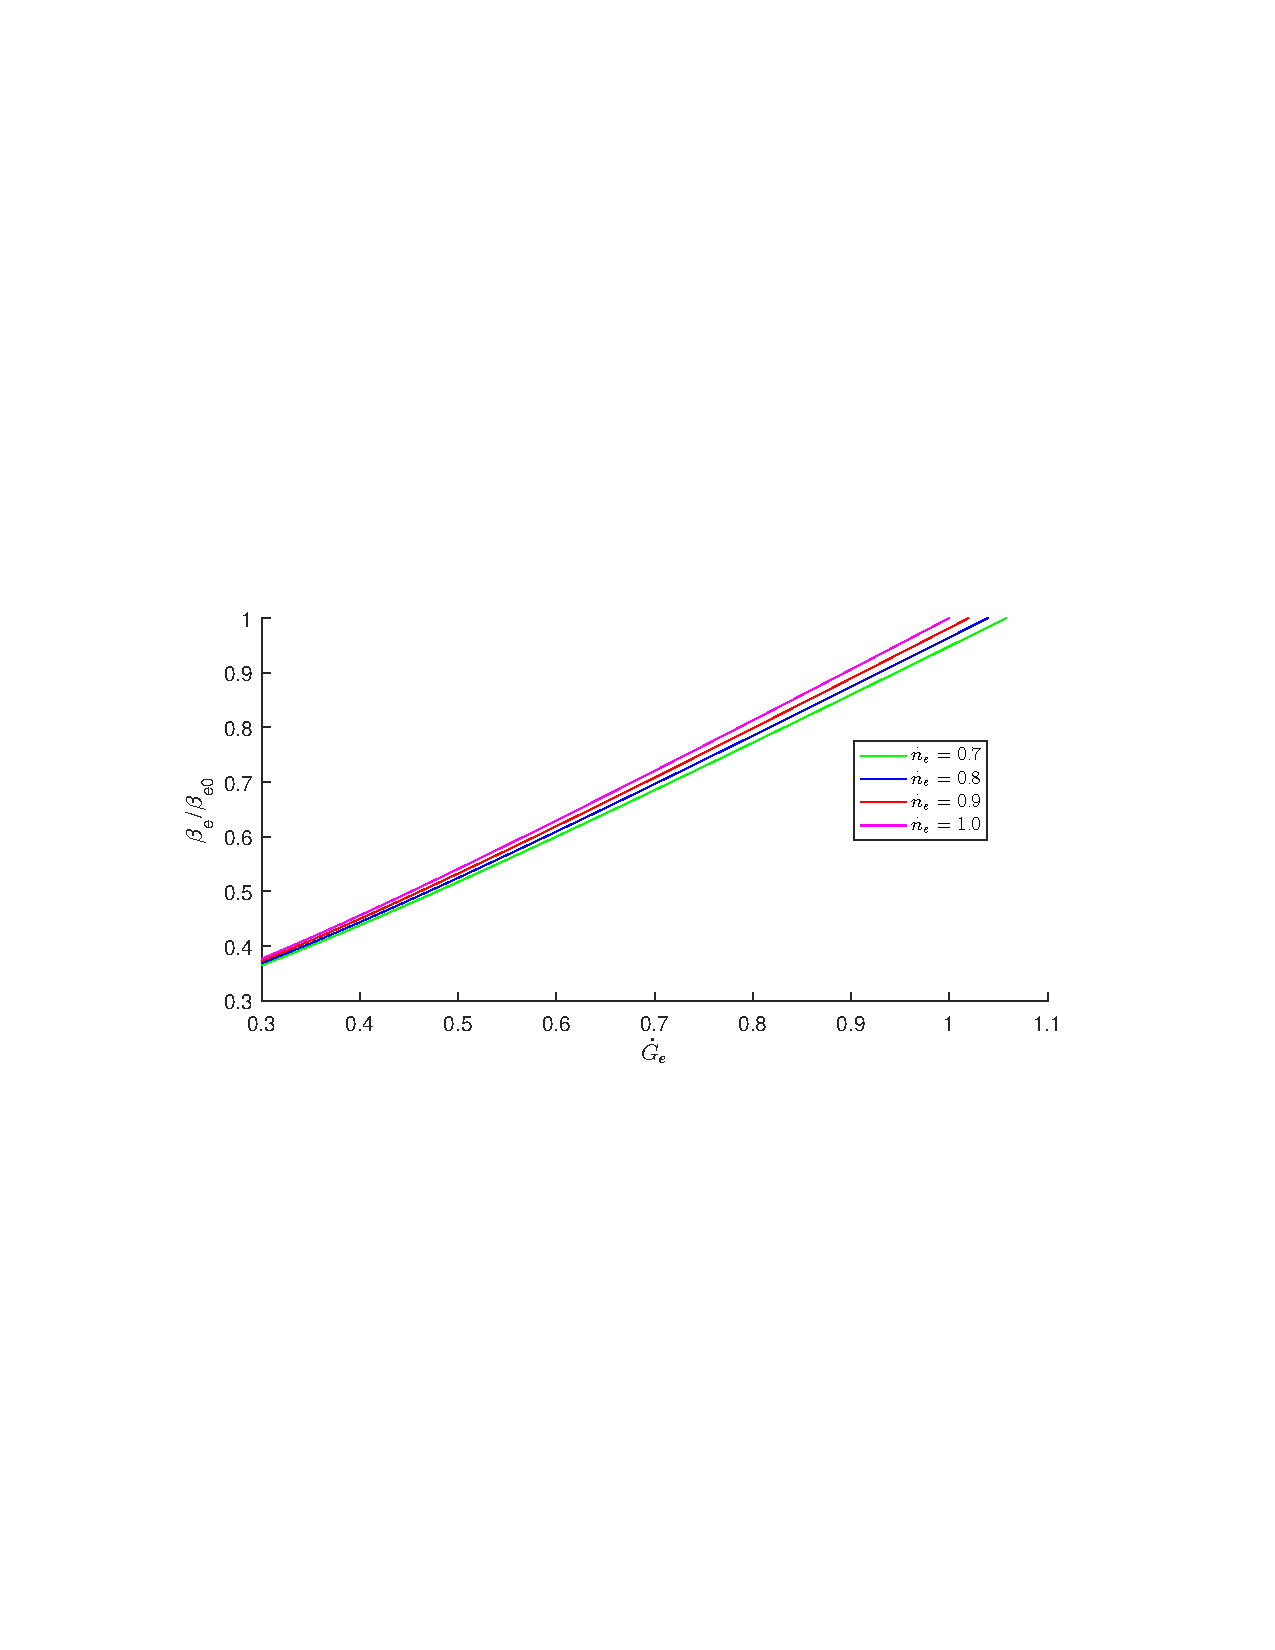
\includegraphics[scale=0.65]{figures/Chap2-2-Turb-Ratio-off-design.pdf}
  \caption{基于解析模型的空气透平部分负载膨胀比}
  \label{fig:Turb-Ratio-off-design}
\end{figure}

\begin{figure}[H] % use float package if you want it here
  \centering
  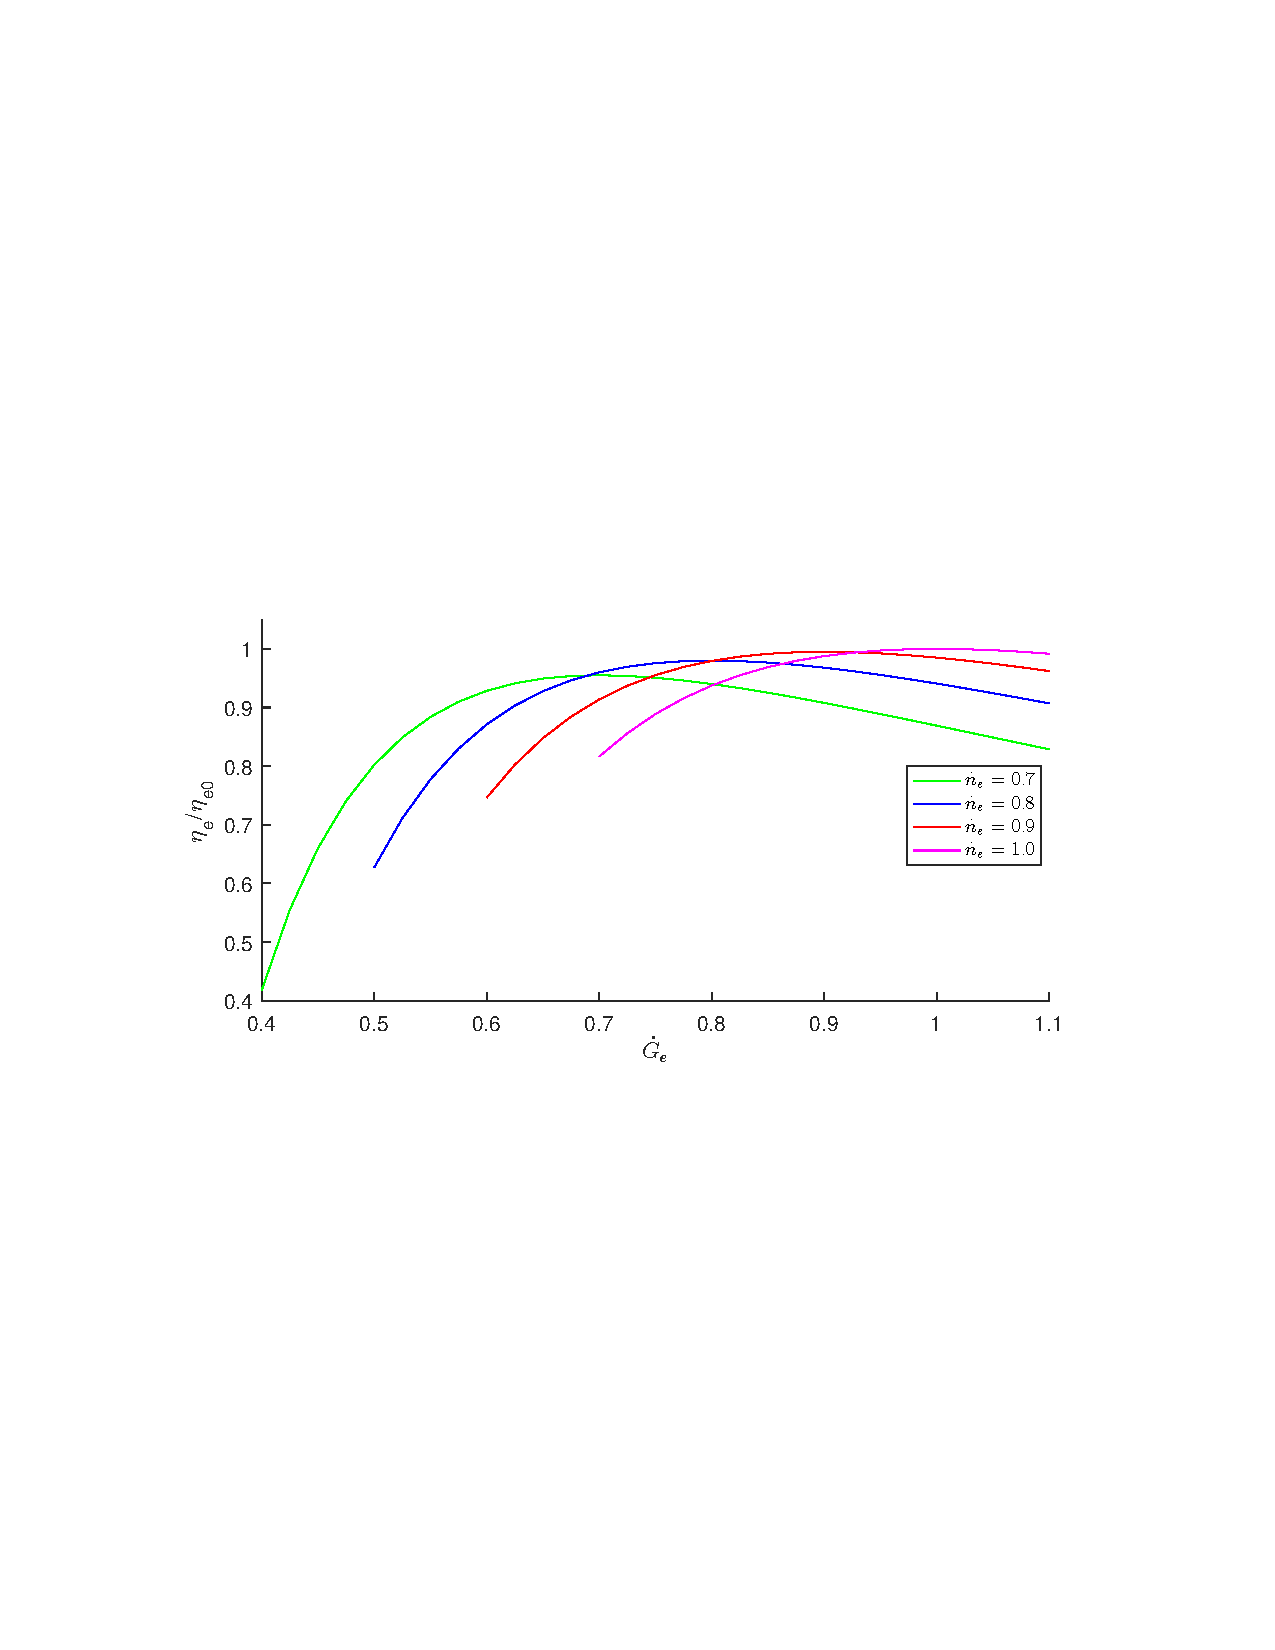
\includegraphics[scale=0.65]{figures/Chap2-3-Turb-Eff-part-load.pdf}
  \caption{基于解析模型的空气透平部分负载等熵效率}
  \label{fig:Turb-Eff-part-load}
\end{figure}

综上,透平的额定工况热力学模型(\ref{equ:turb-real-temp-2})-(\ref{equ:turb-pressure})及部分负载热力学模型(\ref{equ:turb-real-temp-2})-(\ref{equ:turb-pressure-part}) 中的变量如表~\ref{tab:turb-thermo-para}~所示。在实际运行中的任一给定时刻,外界电网调度指令会给出实时功率需求$W_e$,其它边界条件可通过后续组件确定。

\begin{table}[htb]
  \centering
  \begin{minipage}[t]{0.9\linewidth} % 如果想在表格中使用脚注,minipage是个不错的办法
  \caption{空气透平部分负载热力学模型变量表}
  \label{tab:turb-thermo-para}
    \begin{tabularx}{\linewidth}{cccccc}
      \toprule[1.5pt]
      {\heiti 变量} & {\heiti 物理意义} & {\heiti 单位} &  {\heiti 变量} & {\heiti 物理意义} & {\heiti 单位} \\\midrule[1pt]
      ${W_{e,i}}$ & 做功(电) & kW  &  ${\dot m_e}$ & 空气质量流率 & kg/s \\
      ${\beta _{e,i}}$ & 实际膨胀比 & —— &  ${\eta _{e,i}}$ & 等熵效率 & —— \\
      $p_{e,i}^{in}$ & 空气进口压力 & kPa & $p_{e,i}^{out}$ & 空气出口压力 & kPa \\
      $T_{e,i}^{in}$ & 空气进口温度 & K & $T_{e,i}^{out}$ & 空气出口温度 & K \\
      ${n_{e,i}}$ & 实际转速 & r/min & $\dot n_{e,i}$ & 无量纲降阶转速 & —— \\
      ${\dot G_{e,i}}$ &  无量纲降阶质量流率 &  —— & & & \\
      \bottomrule[1.5pt]
    \end{tabularx}
  \end{minipage}
\end{table}

\subsection{能量转移类模块}
\label{sec:part-load-energy-he}

对AA-CAES各应用形式而言,一般均含有压缩侧换热器与膨胀侧换热器等能量转移类模块,本小节分别给出二者在额定工况及部分负载工况下的稳态热力学模型。

\subsubsection{压缩侧换热器}
定义第$i$ 级换热器的空气侧入口温度为 $T_{c,HX,i}^{a,in}$ ,载热工质(Heat Transfer Fluid, HTF)的入口温度为$T_{c,HX,i}^{HTF,in}$,则换热器出口侧空气温度及HTF 温度分别为\cite{CAES-Wind-Rui-19}
\begin{subequations}
\label{eq:he-comp-temp-out}
\begin{gather}
T_{c,HX,i}^{a,out} = T_{c,HX,i}^{a,in} + \Phi _{c,i}^{HX}/({c_p^a\dot m_c^a}) \label{equ:he-comp-temp-air-out} \\
T_{c,HX,i}^{HTF,out} = T_{c,HX,i}^{HTF,in} - \Phi _{c,i}^{HX}/({c_p^{HTF}\dot m_{c,i}^{HTF}}) \label{equ:he-comp-temp-HTF-out}\\
\Phi _{c,i}^{HX} = {\varepsilon _{c,i}}C_{c,i}^{\min }({T_{c,HX,i}^{HTF,in} - T_{c,HX,i}^{a,in}})\label{equ:he-comp-thermal}
\end{gather}
\end{subequations}
其中,$\dot m_{c,i}^{HTF}$ 为HTF质量流率;$c_p^{HTF}$为HTF 定压比热容;$\Phi _{c,i}^{HX}$ 为换热器的换热功率;$C_{c,i}^{\min}$为换热器最小热容;${\varepsilon _{c,i}}$ 为换热器效能,具体表达式视实际换热器类型而定,图\ref{fig:CAES-thermal-struc}中压缩侧采用的逆流换热器的效能${\varepsilon _{c,i}}$ 满足\cite{Heat-mass-transfer-11}:
\begin{subequations}
\begin{gather}
{\varepsilon _{c,i}} = \frac{{1 - \exp [{ - NT{U_{c,i}}({1 - C_{c,i}^{HX}})}]}}{{1 - C_{c,i}^{HX}\exp [{ - NT{U_{c,i}}({1 - C_{c,i}^{HX}})}]}}\label{equ:he-comp-eff-1}
%{\varepsilon _{c,i}} = \frac{{1 - \exp \left[ { - NT{U_{c,i}}\left( {1 + C_{c,i}^{HX}} \right)} \right]}}{{1 + C_{c,i}^{HX}}}\label{equ:he-comp-eff-2}
\end{gather}
\end{subequations}
其中,$NT{U_{c,i}}$ 与$C_{c,i}^{HX}$分别为换热器的传热单元数与热容比,满足\cite{Heat-mass-transfer-11}:
\begin{subequations}
\begin{gather}
NT{U_{c,i}} = U_{c,i}A_{c,i}/C_{c,i}^{\min }, C_{c,i}^{HX} = C_{c,i}^{\min }/C_{c,i}^{\max }\label{equ:he-comp-NTU-C}\\
C_{c,i}^{\min } = {({{{\dot m}_c}c_p^a,\dot m_{c,i}^{HTF}c_p^{HTF}})_{\min }}\label{equ:he-comp-Cmin}\\
C_{c,i}^{\max } = {({{{\dot m}_c}c_p^a,\dot m_{c,i}^{HTF}c_p^{HTF}})_{\max }}\label{equ:he-comp-Cmax}
\end{gather}
\end{subequations}
其中,$C_{c,i}^{\max }$为换热器最大热容;$U_{c,i}$与$A_{c,i}$分别为换热系数与换热面积,不考虑部分负载特性时,$U_{c,i}$可视为常数。

第$i$级换热器所需的HTF的质量流率满足:
\begin{equation}
\label{equ:he-comp-mass-flow}
\dot m_{c,i}^{HTF} = \frac{{{{\dot m}_c}c_p^a({T_{c,HX,i}^{a,in} - T_{c,HX,i}^{a,out}} )}}{{c_p^{HTF}( {T_{c,HX,i}^{HTF,out} - T_{c,HX,i}^{HTF,in}})}}
\end{equation}

考虑换热器的压损特性,则换热器出口的空气压力为
\begin{subequations}
\begin{gather}
p_{c,HX,i}^{out} = \eta _{c,HX,i}^pp_{c,HX,i}^{in}\label{equ:he-comp-pressure-out}
\end{gather}
\end{subequations}
其中,$\eta _{c,HX,i}^p$为换热器压力的保持系数\cite{Thesis-Lixuemei},且满足$\eta _{c,HX,i}^p = 1 - \frac{{0.0083{\varepsilon _{c,i}}}}{{1 - {\varepsilon _{c,i}}}}$,系数0.0083可视实际换热器类型进行调整;若不考虑压损,设置$\eta _{c,HX,i}^p$ 取为1即可。考虑到换热器HTF侧一般由升压泵等调节压力,且其耗功很小,本文仿真模型中不关注HTF侧的压力等信息。

根据质量守恒与能量守恒(温度混合方程),各级换热器汇合后的HTF质量流率及温度分别为
\begin{subequations}
\begin{gather}
\dot m_c^{HTF} = \sum\limits_{i = 1}^{{N_c}} {\dot m_{c,i}^{HTF}} \label{equ:he-comp-mix-mass-flow}\\
T_{c,HX}^{Merge} = {{\sum\limits_{i = 1}^{{N_c}} {\dot m_{c,HX,i}^{HTF}T_{c,HX,i}^{HTF,out}} }}/{{\sum\limits_{i = 1}^{{N_c}} {\dot m_{c,HX,i}^{HTF}}}}  \label{equ:he-comp-mix-temp}
\end{gather}
\end{subequations}

事实上,当流经换热器的高温空气质量流率偏离设计值时,换热器将处于部分负载运行工况,其换热系数$U_{c,i}$将发生较大变化,如图~\ref{fig:HE-Part-Load}~所示
\cite{HE-Eff-CN-17,CAES-Review-18-Rui-operation},从而会影响换热功率$\Phi _{c,i}^{HX}$及出口侧的空气温度与HTF温度。

\begin{figure}[H] % use float package if you want it here
  \centering
  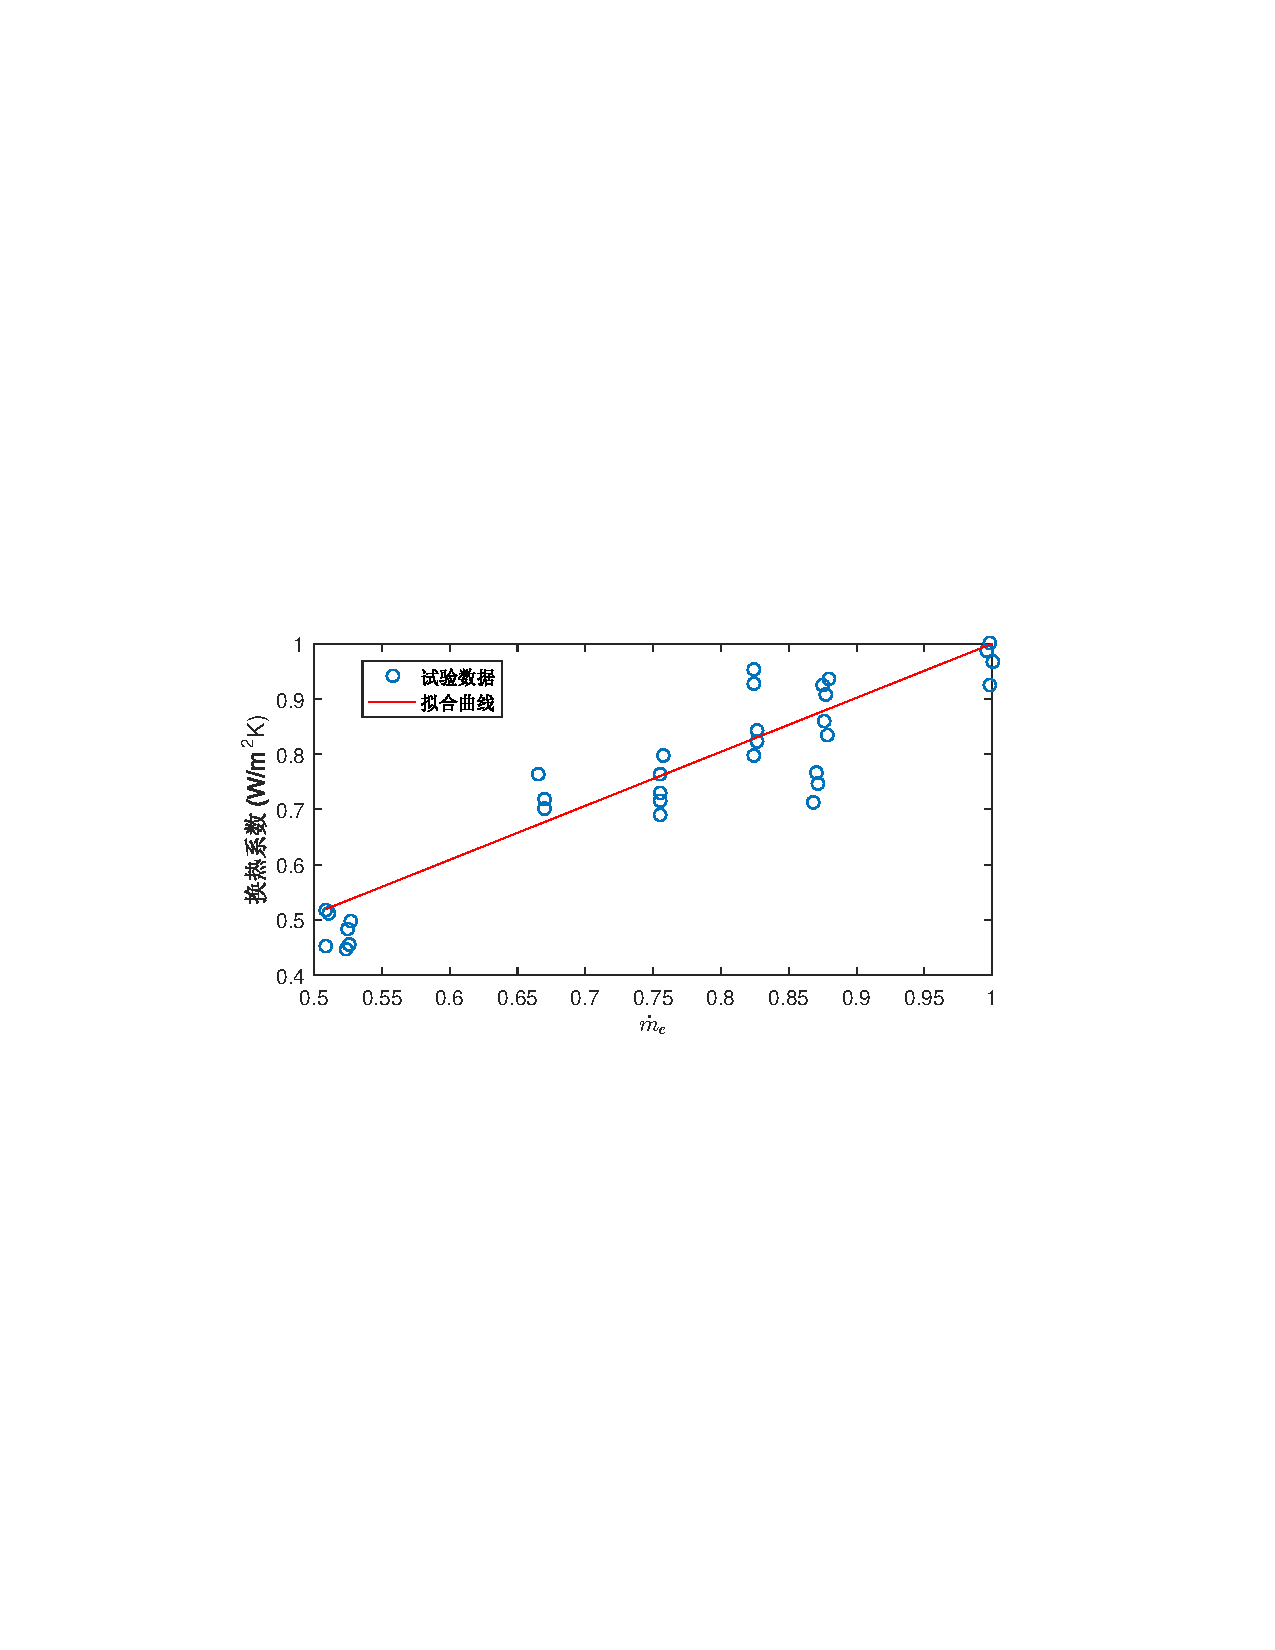
\includegraphics[scale=0.75]{figures/Chap1-7-HE-Part-Load.pdf}
  \caption{换热器换热系数的部分负载特性}
  \label{fig:HE-Part-Load}
\end{figure}

综上,换热器部分负载热力学模型包含的变量如表~\ref{tab:HE-comp-thermo-para}~所示,其边界条件如入口空气温度及压力均可由对应级的压缩机参数给定,同时空气侧质量流率与对应级压缩机的空气质量流率相同,因此其它变量可唯一给定。

\begin{table}[htb]
  \centering
  \begin{minipage}[t]{0.9\linewidth} % 如果想在表格中使用脚注,minipage是个不错的办法
  \caption{压缩侧换热器部分负载热力学模型变量表}
  \label{tab:HE-comp-thermo-para}
    \begin{tabularx}{\linewidth}{cccccc}
      \toprule[1.5pt]
      {\heiti 变量} & {\heiti 物理意义} & {\heiti 单位} &  {\heiti 变量} & {\heiti 物理意义} & {\heiti 单位} \\\midrule[1pt]
      $T_{c,HX,i}^{a,in}$ & 空气侧入口温度 & K  &  $T_{c,HX,i}^{a,out}$ & 空气侧出口温度 & K \\
      $T_{c,HX,i}^{HTF,in}$ & HTF侧入口温度 & K & $T_{c,HX,i}^{HTF,out}$ & HTF侧出口温度 & K \\
      $p_{c,HX,i}^{in}$ & 空气进口压力 & kPa & $p_{c,HX,i}^{out}$ & 空气出口压力 & kPa \\
      $\Phi _{c,i}^{HX}$ & 实际换热功率 & kW & ${\varepsilon _{c,i}}$ & 实际效能& ——  \\
      $NT{U_{c,i}}$ & 实际传热单元数 & —— & $C_{c,i}^{HX}$ &  实际热容比 &  —— \\
      $\eta _{c,HX,i}^p$ & 压力保持系数 & —— & $\dot m_c^{HTF}$ & 汇合后HTF流率 & kg/s\\
      $\dot m_{c,HX,i}^{HTF}$ & 载热流体流率 & kg/s & $C_{c,i}^{\max }$ & 最大热容 & kJ/s/K\\
      $C_{c,i}^{\min }$ & 最小热容 & kJ/s/K & $T_{c,HX}^{Merge}$ & 汇合后HTF温度 & K\\
      \bottomrule[1.5pt]
    \end{tabularx}
  \end{minipage}
\end{table}

\subsubsection{膨胀侧换热器}
定义第$i$ 级换热器的空气侧入口温度为 $T_{e,HX,i}^{a,in}$ ,HTF的入口温度为$T_{e,HX,i}^{HTF,in}$,则换热器出口侧空气温度及HTF温度分别为
\begin{subequations}
\label{eq:he-turb-temp-out}
\begin{gather}
T_{e,HX,i}^{a,out} = T_{e,HX,i}^{a,in} + \Phi _{e,i}^{HX}/({c_p^a\dot m_e^a})\label{equ:he-turb-temp-air-out}\\
T_{e,HX,i}^{HTF,out} = T_{e,HX,i}^{HTF,in} - \Phi _{e,i}^{HX}/({c_p^{HTF}\dot m_{e,i}^{HTF}}) \label{equ:he-turb-temp-HTF-out}\\
\Phi _{e,i}^{HX} = {\varepsilon _{e,i}}C_{e,i}^{\min }({T_{e,HX,i}^{HTF,in} - T_{e,HX,i}^{a,in}})\label{equ:he-turb-thermal}
\end{gather}
\end{subequations}
其中,$\dot m_{e,i}^{HTF}$为膨胀侧第$i$级换热器的质量流率;$\Phi _{e,i}^{HX}$ 为换热器实际换热功率;${\varepsilon _{e,i}}$ 为换热器效能,对于图
\ref{fig:CAES-thermal-struc}中膨胀侧采用的逆流换热器,其效能为\cite{Heat-mass-transfer-11}
\begin{subequations}
\begin{gather}
{\varepsilon _{e,i}} = \frac{{1 - \exp [{- NT{U_{e,i}}({1 - C_{e,i}^{HX}})}]}}{{1 - C_{e,i}^{HX}\exp [{- NT{U_{e,i}}({1 - C_{e,i}^{HX}})}]}}\label{equ:he-eff-1}
%{\varepsilon _{e,i}} = \frac{{1 - \exp \left[ { - NT{U_{e,i}}\left( {1 + C_{e,i}^{HX}} \right)} \right]}}{{1 + C_{e,i}^{HX}}}\label{equ:he-turb-eff-2}
\end{gather}
\end{subequations}
其中,除下标$e$表示膨胀侧外,$NT{U_{e,i}}$ 与$C_{e,i}^{HX}$的含义与压缩侧换热器相同,且满足:
\begin{subequations}
\begin{gather}
NT{U_{e,i}} = U_{e,i}A_{e,i}/C_{e,i}^{\min }, C_{e,i}^{HX} = C_{e,i}^{\min }/C_{e,i}^{\max }\label{equ:he-turb-NTU-C}\\
C_{e,i}^{\min } = {({{{\dot m}_e}c_p^a,\dot m_{e,i}^{HTF}c_p^{HTF}})_{\min }}\label{equ:he-turb-Cmin}\\
C_{e,i}^{\max } = {({{{\dot m}_e}c_p^a,\dot m_{e,i}^{HTF}c_p^{HTF}})_{\max }}\label{equ:he-turb-Cmax}
\end{gather}
\end{subequations}
其中, $C_{e,i}^{\max }$与$C_{e,i}^{\min }$的含义同压缩侧。

第$i$级换热器所需的换热介质的质量流率满足:
\begin{equation}
\label{equ:he-turb-mass-flow}
\dot m_{e,i}^{HTF} = \frac{{{{\dot m}_e}c_p^a({T_{e,HX,i}^{a,in} - T_{e,HX,i}^{a,out}})}}{{c_p^{HTF}({T_{e,HX,i}^{HTF,out} - T_{e,HX,i}^{HTF,in}})}}
\end{equation}

与压缩侧换热器类似,引入换热器压力保持系数\cite{Thesis-Lixuemei}后换热器的出口空气压力为
\begin{subequations}
\begin{gather}
%\eta _{e,HX,i}^p = 1 - \frac{{0.0083{\varepsilon _{e,i}}}}{{1 - {\varepsilon _{e,i}}}}\label{equ:he-turb-pressure-discount}\\
p_{e,HX,i}^{out} = \eta _{e,HX,i}^pp_{e,HX,i}^{in}\label{equ:he-turb-pressure-out}
\end{gather}
\end{subequations}

此外,膨胀侧各级换热器汇合后的HTF质量流率及温度分别为
\begin{subequations}
\begin{gather}
\dot m_e^{HTF} = \sum\limits_{i = 1}^{{N_e}} {\dot m_{e,i}^{HTF}} \label{equ:he-turb-mix-mass-flow}\\
T_{e,HX}^{Merge} = {{\sum\limits_{i = 1}^{{N_e}} {\dot m_{e,HX,i}^{HTF}T_{e,HX,i}^{HTF,out}} }}/{{\sum\limits_{i = 1}^{{N_e}} {\dot m_{e,HX,i}^{HTF}} }}\label{equ:he-turb-mix-temp}
\end{gather}
\end{subequations}

与压缩侧换热器类似,换热系数$U_{e,i}$随部分负载工况的变化明显,导致${\varepsilon _{e,i}}$ 及$\Phi _{e,i}^{HX}$的变化,从而影响透平膨胀机的入口空气温度。

综上,膨胀侧换热器部分负载热力学模型中的变量如表~\ref{tab:HE-turb-thermo-para}~所示,其边界条件如入口空气温度及压力均可由对应级的膨胀机参数给定,同时空气侧质量流率与对应级膨胀机的空气质量流率相同,因此相关其它变量可唯一给定。

\begin{table}[htb]
  \centering
  \begin{minipage}[t]{0.9\linewidth} % 如果想在表格中使用脚注,minipage是个不错的办法
  \caption{膨胀侧换热器部分负载热力学模型变量表}
  \label{tab:HE-turb-thermo-para}
    \begin{tabularx}{\linewidth}{cccccc}
      \toprule[1.5pt]
      {\heiti 变量} & {\heiti 物理意义} & {\heiti 单位} &  {\heiti 变量} & {\heiti 物理意义} & {\heiti 单位} \\\midrule[1pt]
      $T_{e,HX,i}^{a,in}$ & 空气侧入口温度 & K  &  $T_{e,HX,i}^{a,out}$ & 空气侧出口温度 & K \\
      $T_{e,HX,i}^{HTF,in}$ & HTF侧入口温度 & K & $T_{e,HX,i}^{HTF,out}$ & HTF侧出口温度 & K \\
      $p_{e,HX,i}^{in}$ & 空气进口压力 & kPa & $p_{e,HX,i}^{out}$ & 空气出口压力 & kPa \\
      $\Phi _{e,i}^{HX}$ & 实际换热功率 & kW & ${\varepsilon _{e,i}}$ & 实际效能& ——  \\
      $NT{U_{e,i}}$ & 实际传热单元数 & —— & $C_{e,i}^{HX}$ &  实际热容比 &  —— \\
      $\eta _{e,HX,i}^p$ & 压力保持系数 & —— & $\dot m_e^{HTF}$ &  汇合后HTF流率 & kg/s\\
      $\dot m_{e,HX,i}^{HTF}$ & 载热流体流率 & kg/s & $C_{e,i}^{\max }$ & 最大热容 & kJ/s/K\\
      $C_{e,i}^{\min }$ & 最小热容 & kJ/s/K & $T_{e,HX}^{Merge}$ & 汇合后HTF温度 & K\\
      \bottomrule[1.5pt]
    \end{tabularx}
  \end{minipage}
\end{table}

\subsection{能量存储类模块}
对AA-CAES各应用形式而言,一般均包含储热罐及储气库等能量存储类模块,本小节分别给出二者的热力学动态模型。

\subsubsection{储热罐}
\label{sec:TES-thermo-model}
根据压缩机级数及压缩机出口高压空气温度的不同,AA-CAES中压缩热能的存储可分为高温压缩热能存储(400$^{\circ}$C以上)~\cite{A-CAES-Dynamic-17,AA-CAES-07}、中温压缩热能存储(200$^{\circ}$C-400$^{\circ}$C)~\cite{ACAES-Packed-TES} 及低温压缩热能存储(200$^{\circ}$C以下)~\cite{TICC-16}等。相应地,储热技术的种类也较多~\cite{TES-CSP-review-13},AA-CAES各典型实现形式可采用的储热技术主要包括回热式双罐液态储热\cite{TICC-15}或填充床储热\cite{A-CAES-Dynamic-17}、混凝土储热\cite{Model-AA-CAES-10}及相变材料储热\cite{AA-CAES-Simulation-19}等方式。

本章针对常用的回热式双罐液态储热方式建立动态模型,该类储热方式已在我国多座AA-CAES试验系统中普遍使用,如TICC-500\cite{TICC-15}、STHC-100\cite{ST-CAES-17}以及江苏金坛AA-CAES国家示范电站\cite{CAES-Review-17-Rui-salt},同时也在集中式光热电站技术中广泛使用\cite{TES-CSP-review-13}。对于填充层储热结构,可采用文献~\inlinecite{A-CAES-Dynamic-17} 中的动态模型;对于蓄热式混凝土储热罐动态结构,可采用文献~\inlinecite{Model-AA-CAES-10} 中的动态模型;对于相变材料储热,其动态模型可参考文献~\inlinecite{AA-CAES-Simulation-19}。

%\subsubsection{双罐回热结构}
对于图~\ref{fig:CAES-thermal-struc}中所采用的双罐回热储热结构,低温储热罐一般通过与外界充分散热保持恒温,可视为等温;高温储热罐需尽可能减少传热损失,则高温储热罐中储热介质的温度满足\cite{CAES-Wind-Rui-19}:
%其储热模型可建立如下:
%\subsubsection{蓄热式储热结构}
%本章先探讨蓄热式混凝土储热罐动态模型,建模思路可推广至其他类型的储热系统的建模过程。考虑文献~\inlin%ecite{Model-AA-CAES-10}中的带沉浸式换热器线圈的储热系统,如图~\ref{fig:TES-struc-2}~所示。
%\begin{figure}[H] % use float package if you want it here
%  \centering
%  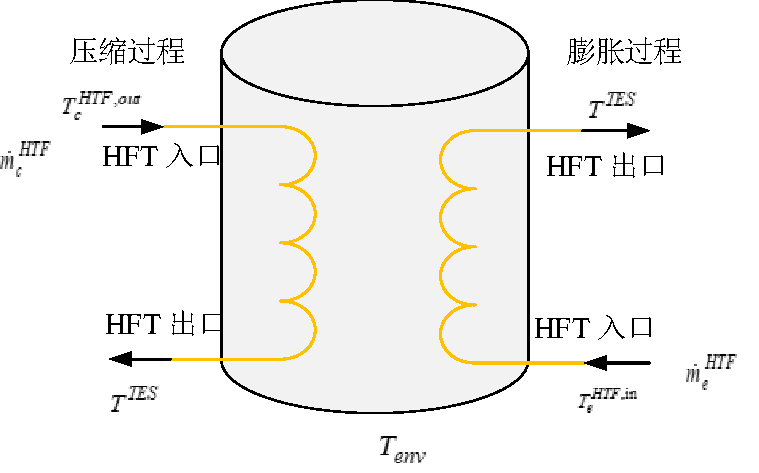
\includegraphics[scale=0.75]{Chap2-4-TES1-Structure}
%  \caption{带沉浸式换热线圈的储热系统示意图}
%  \label{fig:TES-struc-2}
%\end{figure}
\begin{equation}
\label{equ:TES-HTF-temp}
\begin{array}{l}
({{\rho _{TES}}{V_{TES}}c_p^{TES}})\frac{{d{T_{TES}}}}{{dt}} = \dot m_c^{HTF}c_p^{HTF}({T_{c,TES}^{HTF,in} - {T_{TES}}})\\
\;\;\;\;\;\;\;\;\;\;\;\;\;\;\;\;\;\;\;\;\;\;\;\;\; - \dot m_e^{HTF}c_p^{HTF}({{T_{TES}} - T_{e,TES}^{HTF,in}}) - {U_{TES}}{A_{TES}}({{T_{TES}} - {T_{env}}})
\end{array}
\end{equation}
其中,${\rho _{TES}}$ 为储热介质的密度;${V_{TES}}$ 为储热介质的体积;$c_p^{TES}$ 为储热介质的比热容;$T_{c,TES}^{HTF,in}$ 为压缩阶段HTF的出口温度,即$T_{c,HX}^{Merge}$;$T_{e,TES}^{HFT,in}$ 为膨胀阶段HTF的入口温度;${U_{TES}}$与${A_{TES}}$ 分别为储热罐与环境间的传热系数及储热罐的外部表面积,若不考虑传热损失,可令${U_{TES}}$为0;$T_{env}$ 为环境温度。一般情况下,储热介质可选用HTF(如TICC-500采用加压水),也可不同于HTF(如集中式光热电站),本文假定储热介质选用HTF。

\subsubsection{储气库}
\label{sec:Air-tank-thermo-model}
~AA-CAES~可采用的储气方式主要包括压力控制型(即等压储气库)\cite{Isobaric-ACAES-18,Thesis-Wangzhiwen}与容积控制型(即等容储气库)\cite{TICC-15,Thesis-JaiDuhan}两种。本文重点关注较为常见且对地理条件依赖性较小的容积控制型储气库,包括压力容器\cite{TICC-15}、盐穴储气\cite{CAES-Review-17-Rui-salt}、管线钢\cite{ST-CAES-CN-16-Rui}等,如图~\ref{fig:CAES-thermal-struc}中采用的储气库。对于容积控制型储气库,大多研究假定储气库为恒温,如文献~\inlinecite{CAES-Discharge-16}基于恒温储气库模型,研究了D-CAES的两种膨胀侧运行模式;文献~\inlinecite{CAES-CCHP-off-design-18} 基于恒温储气库模型研究了基于AA-CAES的CCHP系统的不同运行模式。然而,实际过程中随着压缩与膨胀过程中高压空气的注入及排出,以及储气库与周围环境之间的换热量的变化,储气库内空气的压力及温度均会发生变化,从而影响压缩储能过程中末级压缩机背压(无入口侧节流阀时)与膨胀释能过程中透平入口空气温度及压力(无出口侧节流阀时)等热力学参数。为此,本文基于文献~\inlinecite{Model-AA-CAES-10} 及文献~\inlinecite{Cavern-model-12}中的温度与压力动态模型,建立储气库通用热力学仿真模型。

\textbf{(1)通用定容模型}

通用定容模型(记为G模型)假定储气库内空气的温度与压力均随压缩储能及膨胀释能过程变化,同时计及储气库与周围环境的换热过程。如此,通用定容储气库的热力学动态模型为\cite{Model-AA-CAES-10,Cavern-model-12,CAES-Wind-Rui-19}
\begin{subequations}
\label{equ:Air-tank-model-G}
\begin{gather}
   \frac{{d{m_{as}}}}{{dt}} = \dot m_{as}^{in} - \dot m_{as}^{out}\\
   \frac{{d{T_{as}}}}{{dt}} = \frac{1}{{{m_{as}}}}[ {({1 - \frac{1}{k}})({\dot m_{as}^{in}T_{as}^{in} - \dot m_{as}^{out}T_{as}^{}})} ] + \frac{{{\alpha _w}{A_w}({{T_w} - {T_{as}}})}}{{{m_{as}}c_p^a}}\label{equ:Air-tank-model-G-T}\\
   \frac{{d{p_{as}}}}{{dt}} = \frac{{k{R_g}}}{{{V_{as}}}}({\dot m_{as}^{in}T_{as}^{in} - \dot m_{as}^{out}T_{as}^{}}) + \frac{{{R_g}}}{{c_v^a{V_{as}}}}{\alpha _w}{A_w}({{T_w} - {T_{as}}} )\label{equ:Air-tank-model-G-P}
\end{gather}
\end{subequations}
其中,${m_{as}}$ 为储气库中的高压空气质量;$\dot m_{as}^{in}$ 与$\dot m_{as}^{out}$分别为储气库的进口空气质量流率与出口空气质量流率;$T_{as}^{in}$与 $T_{as}$ 分别为储气库的进口空气温度与出口空气温度(或储气库的实时空气温度);${A_w}$ 为储气库与周围环境的接触面积; ${T_w}$ 为储气库壁面温度,可采用一维热传导方程求解;$p_{as}(t)$为储气库空气压力;$R_g$为通用气体常数;${\alpha _w}$ 为储气库外表面与环境间的传热系数,其值与储气库的特性有关,如文献~\inlinecite{CAES-Huntorf-12}基于实测Huntorf 电站数据仿真拟合得到了适用于地下盐穴储气库的可变传热系数:
\begin{equation}
\label{equ:wall-thermal-coef}
{\alpha _w} = 0.02356 + 0.0149{\left| {\dot m_{as}^{in} - \dot m_{as}^{out}} \right|^{0.8}}
\end{equation}

事实上,储气库内空气的实时压力$p_{as}$亦可基于空气温度$T_{as}$和质量$m_{as}$,并结合理想气体状态方程求解,即(\ref{equ:Air-tank-model-G}) 存在冗余项。为了描述壁面换热对储气库内空气的热力学特性(温度及压力)的影响,此处给出了二者的具体表达式。从温度动态方程(\ref{equ:Air-tank-model-G-T})及压力动态方程(\ref{equ:Air-tank-model-G-P})可知,储气库(出口)空气温度受进出口空气质量流率及储气库与周围环境的传热过程共同影响,在较大质量流率充气与放气过程中,前者对储气库内空气温度与压力的变化影响较大;在较小质量流率充放气过程中,如压缩机与膨胀机部分负载运行时,储气库与周围环境的传热过程对储气库内空气温度与压力的变化贡献较大\cite{CAES-Wind-Rui-19},这一现象已在基于盐穴储气的Huntorf D-CAES电站实际运行中得到验证\cite{Huntorf-20-01}。 因此,在研究AA-CAES宽工况热力学仿真模型时,通用储气库模型应考虑储气库与周围环境的传热过程。

\textbf{(2)定容等温与绝热模型}

对于非地下盐穴储气等其它小型储气方式而言,储气罐(库)与罐(库)壁的传热损失并不明显,或可通过易于实现的保温、绝热等方式加以控制,此时可在通用定容模型的基础上,进一步简化得到定容等温模型与定容绝热模型。定容等温模型(记为VT模型)假设储气库内空气的温度不随时间变化,从而储气库G模型退化为
\begin{subequations}
\label{equ:Air-tank-model-VT}
\begin{gather}
    \frac{{d{m_{as}}}}{{dt}} = \dot m_{as}^{in} - \dot m_{as}^{out}\\
    \frac{{d{T_{as}}}}{{dt}} = 0\\
    \frac{{d{p_{as}}}}{{dt}} = \frac{{k{R_g}}}{{{V_{as}}}}( {\dot m_{as}^{in}T_{as}^{in} - \dot m_{as}^{out}T_{as}^{}})
\end{gather}
\end{subequations}

类似地,定容绝热储气库模型(记为VA模型)可表示为
\begin{subequations}
\label{equ:Air-tank-model-VA}
\begin{gather}
    \frac{{d{m_{as}}}}{{dt}} = \dot m_{as}^{in} - \dot m_{as}^{out}\\
    \frac{{d{T_{as}}}}{{dt}} = \frac{1}{{{m_{as}}}}[ {({1 - \frac{1}{k}})({\dot m_{as}^{in}T_{as}^{in} - \dot m_{as}^{out}T_{as}^{}} )} ]\\
    \frac{{d{p_{as}}}}{{dt}} = \frac{{k{R_g}}}{{{V_{as}}}}({\dot m_{as}^{in}T_{as}^{in} - \dot m_{as}^{out}T_{as}^{}})
\end{gather}
\end{subequations}


\textbf{(3) 储气库壁面温度求解}

通用定容储气库模型(\ref{equ:Air-tank-model-G})中,$T_{as}$ 及$p_{as}$的求解需要获取墙壁温度$T_w$。$T_w$随储气库内高压空气温度的不同而变化,具体可通过求解一维热传导方程获得\cite{Heat-mass-transfer-11}。如图~\ref{fig:cavern-wall-temp} 所示,定义储气库与墙壁周边任一截面上的温度为$T_{rs}$,由一维热传导方程可得任一时刻任一位置处的温度为~\cite{Heat-mass-transfer-11,Model-AA-CAES-10,Cavern-wall-09}
\begin{equation}
\label{eq:wall-temp}
\frac{{\partial {T_{rs}}\left( {t,r} \right)}}{{\partial t}} = {r_{rs}}({\frac{{{\partial ^2}{T_{rs}}}}{{\partial {r^2}}} + \frac{1}{r}\frac{{\partial {T_{rs}}}}{{\partial r}}})
\end{equation}
其中,${r_{rs}}$为墙壁与储气库的热扩散率。

\begin{figure}[H] % use float package if you want it here
  \centering
  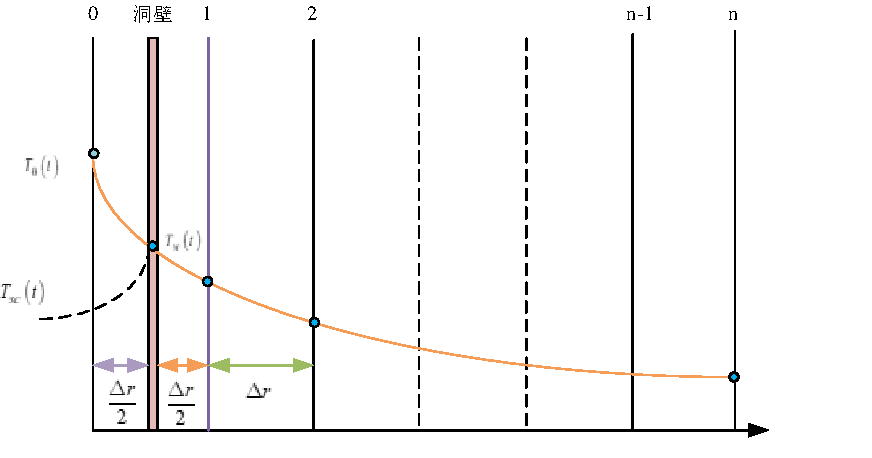
\includegraphics[scale=0.8]{Chap2-5-Wall-Temperature}
  \caption{储气库与洞穴壁温度分布示意图}
  \label{fig:cavern-wall-temp}
\end{figure}

通过求解热传导方程(\ref{eq:wall-temp})的空间离散化方程组(具体求解过程参见附录~\ref{cha:air-wall-temp-exp}),可获取洞穴壁的温度为
\begin{equation}
{T_w}(t) = \frac{{{T_{rs,1}}(t) + {T_{rs,0}}(t)}}{2} = \frac{{{T_{sc,a}}}}{{2({\frac{1}{{B{i^ + }}} + \frac{1}{2}})}} + {T_{rs,1}}({1 - \frac{1}{{({\frac{1}{{B{i^ + }}} + \frac{1}{2}})}}})
\end{equation}
其中,毕奥数(Biot-number) $B{i^ + } = \frac{{{\alpha _{a,w}}\Delta r}}{{{r_{rs}}}}$,${\alpha _{a,w}}$ 表示从空气到洞穴壁的传热系数。

综上,储气库模块的热力学动态模型中的变量如表~\ref{tab:Air-tank-thermo-para}~所示。
\begin{table}[htb]
  \centering
  \begin{minipage}[t]{0.9\linewidth} % 如果想在表格中使用脚注,minipage是个不错的办法
  \caption{储气库热力学动态模型变量表}
  \label{tab:Air-tank-thermo-para}
    \begin{tabularx}{\linewidth}{cccccc}
      \toprule[1.5pt]
      {\heiti 变量} & {\heiti 物理意义} & {\heiti 单位} &  {\heiti 变量} & {\heiti 物理意义} & {\heiti 单位} \\\midrule[1pt]
      ${m_{as}}$ & 储气库中高压空气质量 & Kg  &  $\dot m_{as}^{in}$ & 储气库进口空气流率 & Kg/s \\
      $\dot m_{as}^{out}$ & 储气库出口空气流率 & Kg/s & $T_{as}^{in}$ & 储气库进口空气温度 & K \\
      $T_{as}^{out}/T_{as}$ & 储气库出口空气温度 & K & ${T_w}$ & 墙壁温度 & K \\
      ${p_{as}}$ & 储气库空气实时压力 & kPa & & &\\
      \bottomrule[1.5pt]
    \end{tabularx}
  \end{minipage}
\end{table}

\subsection{运行模式控制模块}
\label{sec:part-load-energy-TV}

AA-CAES四种运行模式的确定可由运行模式控制模块,即储气库入口侧的节流阀及储气库出口侧的节流阀来控制,本小节给出其热力学模型。

一般而言,绝热节流是等焓过程~\cite{Eng-Thermo-83},节流前后空气质量流率相同,温度相同,只有压力不同。因此,流经储气库入口侧节流阀(Throttle Valve, TV)模块的空气满足:
\begin{equation}
    \dot m_{c,TV}^{in} = \dot m_{c,TV}^{out}, T_{c,TV}^{in} = T_{c,TV}^{out}
\end{equation}
节流前后空气的压力由其它边界条件确定。

类似地,流经储气库出口侧的节流阀模块的空气满足:
\begin{equation}
    \dot m_{e,TV}^{in} = \dot m_{e,TV}^{out}, T_{e,TV}^{in} = T_{e,TV}^{out}
\end{equation}
%节流前后压力亦由其它边界条件确定。

综上,节流阀模块热力学模型中的变量如表~\ref{tab:throttle-valve-para}~所示。
\begin{table}[htb]
  \centering
  \begin{minipage}[t]{0.88\linewidth} % 如果想在表格中使用脚注,minipage是个不错的办法
  \caption{节流阀热力学模型变量表}
  \label{tab:throttle-valve-para}
    \begin{tabularx}{\linewidth}{cccccc}
      \toprule[1.5pt]
      {\heiti 变量} & {\heiti 物理意义} & {\heiti 单位} &  {\heiti 变量} & {\heiti 物理意义} & {\heiti 单位} \\\midrule[1pt]
      $\dot m_{c,TV}^{in}$ & 压缩侧TV入口流率 & kg/s &  $\dot m_{c,TV}^{out}$ & 压缩侧TV出口流率 & kg/s \\
      $T_{c,TV}^{in}$ & 压缩侧TV入口温度 & K & $T_{c,TV}^{out}$ & 压缩侧TV出口温度 & K \\
      $p_{c,TV}^{in}$ & 压缩侧TV入口压力 & kPa & $p_{c,TV}^{out}$ & 压缩侧TV出口压力 & kPa \\
      $\dot m_{e,TV}^{in}$ & 透平侧TV入口流率 & kg/s &  $\dot m_{e,TV}^{out}$ & 透平侧TV出口流率 & kg/s \\
      $T_{e,TV}^{in}$ & 透平侧TV入口温度 & K & $T_{e,TV}^{out}$ & 透平侧TV出口温度 & K \\
      $p_{e,TV}^{in}$ & 透平侧TV入口压力 & kPa & $p_{e,TV}^{out}$ & 透平侧TV出口压力 & kPa \\
      \bottomrule[1.5pt]
    \end{tabularx}
  \end{minipage}
\end{table}

\subsection{模型边界条件及性能指标}
\label{sec:part-load-energy-boundary}
边界条件定义了AA-CAES各组件模型之间的关联关系,主要包括压缩侧接口与膨胀侧接口。以下针对图~\ref{fig:CAES-thermal-struc}所示的AA-CAES结构给出其边界条件,其它AA-CAES结构可稍作修改即可。

\subsubsection{压缩侧模型接口}
第$i$级压缩机的入口空气温度与压力分别为环境压力$p_0$与环境温度$T_0$。第$i$级($1\le i<N_c$)压缩机的出口空气温度与压力为第$i$级压缩侧换热器的入口空气温度与压力,第$i$ 级换热器的出口空气压力与温度为第$i+1$级压缩机的入口空气压力与温度,即
\begin{subequations}
\begin{gather}
T_{c,HX,i}^{a,in} = T_{c,i}^{out},T_{c,HX,i}^{a,out} = T_{c,i + 1}^{in},\;\forall 1\le i < {N_c}\\
p_{c,HX,i}^{a,in} = p_{c,i}^{out},p_{c,HX,i}^{a,out} = p_{c,i + 1}^{in},\;\forall 1\le i < {N_c}
%{{\dot m}_c} = \dot m_{as}^{in}
\end{gather}
\end{subequations}

整个压缩侧经过各级压缩机、换热器及节流阀的空气质量流率相同。同时,末级压缩机($i=N_c$)的出口空气压力与温度分别为末级换热器的入口空气压力与温度,末级换热器的出口空气压力与温度则视AA-CAES压缩侧运行模式而不同。具体为:1)压缩侧定压运行模式下
\begin{subequations}
\begin{gather}
\dot m_{c,TV}^{in} = {{\dot m}_c},\dot m_{c,TV}^{out} = \dot m_{as}^{in}\\
T_{c,HX,i}^{a,in} = T_{c,i}^{out},T_{c,HX,i}^{a,out} = T_{c,TV}^{in},T_{c,TV}^{out} = T_{as}^{in}\;,i = {N_c}\\
p_{c,HX,i}^{a,in} = p_{c,i}^{out},p_{c,HX,i}^{a,out} = p_{as}^{\max },\;p_{c,TV}^{in} = p_{as}^{\max },p_{c,TV}^{out} = p_{as}^{},i = {N_c}
\end{gather}
\end{subequations}
2)压缩侧滑压模式下
\begin{subequations}
\begin{gather}
{{\dot m}_c} = \dot m_{as}^{in}\\
T_{c,HX,i}^{a,in} = T_{c,i}^{out},T_{c,HX,i}^{a,out} = T_{as}^{in}\;,i = {N_c}\\
p_{c,HX,i}^{a,in} = p_{c,i}^{out},p_{c,HX,i}^{a,out} = p_{as}^{},\;i = {N_c}
\end{gather}
\end{subequations}
其中,$p_{as}^{max}$为储气库最大工作压力。

第$i$级($1\le i\le {N_c}$)换热器载热流体的入口温度均为定值,为冷罐中的HTF温度,即
\begin{equation}
T_{c,HX,i}^{HTF,in} = T_{cool}^{HTF}
\end{equation}
所有换热器载热流体侧出口温度汇合后的温度为储热罐的入口HTF 温度,即
\begin{equation}
T_{c,HX}^{HTF,Merge} = T_{c,TES}^{HTF,in}
\end{equation}

\subsubsection{膨胀侧模型接口}
第$i$级($1<i\le N_e$)膨胀机的入口空气温度与压力分别为第$i$级膨胀机侧换热器的出口空气温度与压力,第$i$级( $1<i\le N_e$)换热器的入口空气压力与温度分别为第$i-1$ 级膨胀机的出口空气压力与温度,即
\begin{subequations}
\begin{gather}
T_{e,HX,i}^{a,out} = T_{e,i}^{in},T_{e,HX,i}^{a,in} = T_{e,i + 1}^{out},\;\forall 1<i\le N_e\\
p_{e,HX,i}^{a,out} = p_{e,i}^{in},p_{e,HX,i}^{a,in} = p_{e,i + 1}^{out},\;\forall 1<i\le N_e
%{{\dot m}_e} = \dot m_{as}^{out}
\end{gather}
\end{subequations}

整个膨胀侧流经节流阀、各级换热器、膨胀机的空气质量流率相同。同时,首级膨胀机的入口空气压力与温度分别为首级换热器的出口空气压力与温度,首级换热器的入口空气压力与温度则视AA-CAES膨胀侧运行模式而不同。具体地:1)膨胀侧定压运行模式下
\begin{subequations}
\begin{gather}
\dot m_{e,TV}^{out} = {{\dot m}_e},\dot m_{e,TV}^{in} = \dot m_{as}^{out}\\
T_{e,HX,i}^{a,out} = T_{e,i}^{in},T_{e,HX,i}^{a,in} = T_{e,TV}^{out},T_{e,TV}^{in} = T_{as}\;,i = 1\\
p_{e,HX,i}^{a,out} = p_{e,i}^{in},p_{e,HX,i}^{a,in} = p_{as}^{\min },\;p_{e,TV}^{out} = p_{as}^{\min },p_{e,TV}^{in} = p_{as}^{},i = 1
\end{gather}
\end{subequations}
2)膨胀侧滑压运行模式下
\begin{subequations}
\begin{gather}
{{\dot m}_e} = \dot m_{as}^{out}\\
T_{e,HX,i}^{a,out} = T_{e,i}^{in},T_{e,HX,i}^{a,in} = T_{as}^{out}\;,i = 1\\
p_{e,HX,i}^{a,out} = p_{e,i}^{in},p_{e,HX,i}^{a,in} = p_{as}^{out},\;i = 1
\end{gather}
\end{subequations}
其中,$p_{as}^{min}$为储气库最小工作压力。

第$i$级($1\le i\le N_e$)换热器载热流体的入口温度均为定值,为储热罐的HTF出口温度,即
\begin{equation}
T_{e,HX,i}^{HTF,in} = {T_{e,TES}^{HTF,in}}
\end{equation}
所有换热器载热流体侧的出口HTF温度汇合后的温度为冷罐中的HTF 温度,即
\begin{equation}
T_{e,HX}^{HTF,Merge} = T_{cool}^{HTF}
\end{equation}
此外,第$N_e$级膨胀机排气压力需大于$p_0$, 排气温度可视温度的大小,可用于制冷或供暖。

\subsubsection{能量效率指标}
\label{sec:part-load-energy-full}
%本章一定要考虑电动机与发电机的效率,为直接实现第5章机械转矩或机械功的输入或输出建模埋下伏笔与奠定基础。
基于组件级的部分负载热力学模型,可构建AA-CAES系统级的通用宽工况热力学仿真模型,具体包括压缩机、空气透平及换热器的部分负载热力学模型,储热罐与储气库的热力学动态模型,节流阀模型及受控于AA-CAES运行方式的边界条件。

为了分析AA-CAES系统级的性能,定义电效率、热效率及总能利用系数分别为
\begin{equation}
%{\eta _{work}} = \frac{{{\int_0^{t_{dis}}W_e}}}{{{\int_0^{t_{ch}}W_c}}}, {\eta _{hot}} = \frac{{Q_H^L}}{{\int_0^{t_{ch}}{W_c}}}, {\eta _{cool}} = \frac{{Q_C^L}}{{{\int_0^{t_{ch}}W_c}}}
{\eta _{elec}} = \frac{{\int_0^{{t_{dis}}} {{W_e}dt}}}{{{\int_0^{{t_{ch}}} {{W_c}dt}}}}, {\eta _{heat}} = \frac{{Q_H^L}}{{{\int_0^{{t_{ch}}} {{W_c}dt}}}}, {\eta _{total}} = {\eta _{elec}} + {\eta _{heat}}
\end{equation}
%3)定义体积储能密度为
%\begin{equation}
%EVR = \frac{{{E_e}}}{{{V_{as}}}} = %\frac{{\int_0^{{t_{dis}}} {{{W_{e}}}dt} %}}{{{V_{as}}}}
%\end{equation}
其中,$t_{ch}$与$t_{dis}$分别为压缩储能时间与膨胀释能时间;$Q_{H}^{L}$为一个循环周期内AA-CAES对外提供的热能,其具体计算方式视AA-CAES系统结构、供热方式等的不同而异。%本文将在后续针对具体的系统分析中给出其对应的定义。

\section{基于㶲平衡的宽工况热力学模型}
\label{sec:chap2-part-load-exergy}
AA-CAES具有典型的多能流耦合特性,主要表现为对内的空气压缩热能与压力势能双能流间的耦合,以及对外的冷、热、电多能流间的耦合。基于热平衡的宽工况仿真模型难以从统一的视角给出AA-CAES内外多能流间的差异,而基于㶲理论的思路可为分析AA-CAES的多能流特性提供新的视角,本节将给出基于㶲平衡的仿真模型。 事实上,通过第
\ref{sec:part-load-energy}节的热力学仿真模型可以得到AA-CAES宽工况运行时各组件在额定工况或部分负载工况下作功工质(空气、HTF)在各热力学状态点(如图
\ref{fig:CAES-thermal-struc} 中标注的状态点1-12 及$1^*$-$14^*$)的流率、压力、温度等参数,并基于此通过查询工质(空气、HTF等)的热物性表\footnote{热物性表可利用NIST的REFPROP获取,具体可参见https://www.nist.gov/srd/refprop},即可得到对应状态点下的焓值及熵值~\cite{Eng-Thermo-83},进而可建立AA-CAES的㶲平衡模型。

\subsection{压缩机㶲模型}
压缩机的输入㶲为消耗的压缩功,输出㶲为入口与进口空气焓㶲差。如此,第$i$级压缩机的输入㶲与输出㶲分别为\cite{Eng-Thermo-83}
\begin{subequations}
\label{eq:exergy-compressor}
\begin{gather}
Ex_{c,i}^{in} = {W_{c,i}}\label{equ:comp-exergy-in}\\
Ex_{c,i}^{out} = {\dot m_c}[ {c_p^a\left( {T_{c,i}^{out} - T_{c,i}^{in}} \right) - {T_0}({c_p^a\ln \frac{{T_{c,i}^{out}}}{{T_{c,i}^{in}}} - {R_g}\ln \frac{{p_{c,i}^{out}}}{{p_{c,i}^{in}}}})}]\label{equ:comp-exergy-out}
\end{gather}
\end{subequations}

相应地,第$i$级压缩机的㶲损为
\begin{equation}
\label{equ:comp-exergy-loss}
L{x_{c,i}} = Ex_{c,i}^{in} - Ex_{c,i}^{out}
\end{equation}

\subsection{空气透平㶲模型}
透平的输入㶲由空气提供,输出㶲为输出功。如此,进入第$i$级空气透平的输入㶲与输出㶲分别为\cite{Eng-Thermo-83}
\begin{subequations}
\begin{gather}
Ex_{e,i}^{in} = {\dot m_e}[ {c_p^a( {T_{e,i}^{in} - T_{e,i}^{out}}) - {T_0}({c_p^a\ln \frac{{T_{e,i}^{in}}}{{T_{e,i}^{out}}} - {R_g}\ln \frac{{p_{e,i}^{in}}}{{p_{e,i}^{out}}}})}]\label{equ:turb-exergy-in}\\
Ex_{e,i}^{out} = {W_{e,i}}\label{equ:turb-exergy-out}
\end{gather}
\end{subequations}

相应地,第$i$级膨胀机的㶲损为
\begin{equation}
\label{equ:turb-exergy-loss}
L{x_{e,i}} = Ex_{e,i}^{in} - Ex_{e,i}^{out}
\end{equation}

\subsection{换热器㶲模型}

\textbf{(1)压缩侧换热器}

压缩侧换热器的输入㶲由高温空气提供,输出㶲由载热流体带走。如此,进入第$i$级换热器的㶲为
\begin{equation}
\label{equ:he-comp-exergy-in}
Ex_{HX,i}^{c,in} = {\dot m_c}[ {c_p^a({T_{HX,i}^{a,in} - T_{HX,i}^{a,out}}) - {T_0}c_p^a\ln \frac{{T_{HX,i}^{a,in}}}{{T_{HX,i}^{a,out}}}}]
\end{equation}

流出第$i$级换热器的㶲为载热流体带走的㶲,即
\begin{equation}
\label{equ:he-comp-exergy-out}
Ex_{HX,i}^{c,out} = \dot m_{c,i}^{HTF}\left[ {({h_{HX,i}^{HTF,out} - h_{HX,i}^{HTF,in}}) - {T_0}({s_{HX,i}^{HTF,out} - s_{HX,i}^{HTF,in}})}\right]
\end{equation}
其中,$h_{HX,i}^{HTF,in}$与$s_{HX,i}^{HTF,in}$分别为换热器HTF侧的入口焓与熵;$h_{HX,i}^{HTF,out}$与$s_{HX,i}^{HTF,out}$分别为出口焓与熵;$h_{0}^{HTF}$与$s_{0}^{HTF}$分别为参考点的焓与熵\footnote{一般而言,AA-CAES系统中空气、HTF等稳流工质的㶲均需由焓($h$)与熵($s$) 计算。由于本文假设空气为理想气体,其$h$, $s$ 均为温度的单变量函数,故采用温度表示了空气的熵与焓,如(\ref{equ:he-comp-exergy-in}); 而HTF由于种类多,具体类型视特定系统而定,可采用加压水、导热油、熔融盐等,一般不是理想工质,故直接用$h$ 与$s$表示,如(\ref{equ:he-comp-exergy-out})。}。

相应地,第$i$级换热器的㶲损为
\label{equ:he-comp-exergy-loss}
\begin{equation}
Lx_{HX,i}^c = Ex_{HX,i}^{c,in} - Ex_{HX,i}^{c,out}
\end{equation}

\textbf{(2)膨胀侧换热器}

与压缩侧换热器相反,膨胀侧换热器的输入㶲由高温HTF提供,输出㶲由空气带走。如此,流入第$i$级换热器的输入㶲为
\begin{equation}
\label{equ:he-turb-exergy-in}
Ex_{HX,i}^{e,in} = \dot m_{e,i}^{HTF}\left[{({h_{HX,e,i}^{HTF,in} - h_{HX,e,i}^{HTF,out}}) - {T_0}({s_{HX,e,i}^{HTF,in} - s_{HX,e,i}^{HTF,out}})}\right]
\end{equation}
其中,相关变量的含义同压缩侧换热器,下标$e$表示膨胀侧。

流出第$i$级换热器的㶲为空气带走的㶲,即
\begin{equation}
\label{equ:he-turb-exergy-out}
Ex_{HX,i}^{e,out} = {\dot m_{e,i}}[ {c_p^a({T_{HX,i}^{a,e,out} - T_{HX,i}^{a,e,in}}) - {T_0}c_p^a\ln \frac{{T_{HX,i}^{a,e,out}}}{{T_{HX,i}^{a,e,in}}}}]
\end{equation}

相应地,第$i$级换热器的㶲损为
\begin{equation}
\label{equ:he-turb-exergy-loss}
Lx_{HX,i}^e = Ex_{HX,i}^{e,in} - Ex_{HX,i}^{e,out}
\end{equation}

\subsection{节流阀㶲模型}
 节流阀的输入㶲为入口空气的㶲,输出㶲为出口空气的㶲。对于入口侧节流阀而言,输入㶲为末级换热器的出口空气㶲,输出㶲为进入储气库前的高压空气的焓㶲。因此,储气库入口侧及出口侧节流阀的㶲损分别为
\begin{subequations}
\label{eq:exergy-TV}
\begin{gather}
Lx_{TV}^c = Ex_{c,TV}^{in} - Ex_{c,TV}^{out} \label{equ:throttle-valve-comp-exergy-loss}\\
Lx_{TV}^e = Ex_{e,TV}^{in} - Ex_{e,TV}^{out} \label{equ:throttle-valve-turb-exergy-loss}
\end{gather}
\end{subequations}
其中,$Ex_{c,TV}^{in}$为压缩侧末级换热器出口空气的焓㶲;$Ex_{c,TV}^{out}$为储气库入口侧空气的焓㶲;$Ex_{e,TV}^{in}$为储气库出口侧空气的焓㶲; $Ex_{e,TV}^{out}$为膨胀侧首级换热器入口空气的焓㶲;四者均可由对应空气的热力学状态参数(温度、压力)计算得出。
%\begin{equation}
%Ex = \dot mc_p^a\left( {T - {T_0}\ln T} %\right)
%\end{equation}

%\subsection{储气库㶲模型}

%\subsection{储热罐㶲模型}

\subsection{㶲效率指标}
基于热力学第一定律的性能指标可以反映系统内的能量转换情况,但其将功与热等同对待,导致该类效率评价指标只能反映系统能量利用的数量关系,不能反映其在能量利用品位上的不同,难以应用于AA-CAES多能联供应用场景的分析。为此,定义基于热力学第二定律的㶲效率指标以分析系统性能。

基于㶲的电效率、热效率及总㶲效率分别为
\begin{equation}
{\eta _{x,elec}} = \frac{{\int_0^{{t_{dis}}} {Ex_e^{out}dt} }}{{\int_0^{{t_{ch}}} {Ex_c^{in}dt} }},{\eta _{x,heat}} = \frac{{Ex_H^L}}{{\int_0^{{t_{ch}}} {Ex_c^{in}dt} }}, {\eta _x} = {\eta _{x,elec}} + {\eta _{x,heat}}
\end{equation}
其中,${Ex_H^L}$为AA-CAES多能联供的热量㶲。

%为分析方便,引入储气库的㶲存储能力~\cite{Exergy-storage-17},
%\begin{equation}
%Ex_{as}^{\max } = \int_0^{{t_{ch}}} %{\dot E{x_{as}}dt}  = \int_0^{{t_{ch}}} %{{{\dot m}_c}\left\{ {c_p^a\left( %{{T_{as}^{in}} - {T_0}} \right) - %{T_0}\left[ {c_p^a\ln \left( %{\frac{T_{as}}{{{T_0}}}} \right) - R\ln %\left( {\frac{p_{as}}{{{p_0}}}} %\right)} \right]} \right\}dt}
%\end{equation}

%此外,在多能联供场景下,定义制热能效比与制冷能效比
%\begin{equation}
%CO{P_h} = \frac{{Q_H^L}}{{\int_0^{t_{ch%}}{W_cdt} - \int_0^{t_{dis}}{W_edt}}}, %CO{P_c} = \frac{{Q_{\rm{C}}^{\rm{L}}}}{%{\int_0^{t_{ch}}{W_cdt} - %\int_0^{t_{dis}}{W_edt}}}
%\end{equation}
%其中,$\int_0^{t_{ch}}{W_cdt} - \int_0^{t_{dis}}{W_edt}$ 等效表示系统生产热能与冷能所消耗的机械功。

\section{宽工况仿真平台实现及典型系统热力学特性分析}
\label{sec:chap2-bound-measure}

\subsection{宽工况仿真系统的实现}
第\ref{sec:part-load-energy}节中压缩机及空气透平的部分负载热力学模型中引入了压缩机转速$n_c$与透平转速$n_e$,二者分别由与之相连的电动机与发电机的转速及对应的转速控制策略决定。考虑到Matlab/Simulink自带了电力系统仿真模块SIMPOWER,其中的发电机与电动机模块设有转速接口,可直接与本章的压缩机与膨胀机的热力学模型集成。同时,本文第1.2节提出的接口灵活性需挖掘压缩机与膨胀机的机械输入与输出接口,而非电能输入与电能输出接口。因此,为了AA-CAES宽工况仿真模型与电力系统接口的功能拓展以及仿真系统的通用性,本节基于Matlab/Simulink构建如图~\ref{fig:Simulation-Platform} 所示的计及组件部分负载特性的AA-CAES宽工况热力学仿真系统,主要包括压缩机模块(内置压缩侧换热器)、膨胀机模块(内置膨胀侧换热器)、储气库模块、储热罐模块、节流阀模块以及功能控制模块,各模块实现本章所构建的热力学模型及对应的接口条件\footnote{模型中的㶲计算采用了开源Matlab㶲接口程序HOT(Thermodynamic Tools for Matlab),具体可参见http://hot-tdb.sourceforge.net/}。

事实上,正如第\ref{sec:research-state}节分析的AA-CAES的灵活性一样,在不同的结构实现形式中AA-CAES与电力/热力的接口不同,相应的转速控制策略也有所不同,但一般均会采用最优转速控制策略,实现高效运行。为便于分析方便,本节假定实际AA-CAES 实时通过转速$n_c$与$n_e$的调节确保了压缩机与膨胀机在相应运行工况下的最大等熵效率运行,即图\ref{fig:Comp-Ratio-off-design}与图\ref{fig:Eff-part-load} 中的压比与等熵效率可分别表示为质量流率的单值函数,膨胀机与之类似。
%为此,参考热力学仿真工具包Thermolib中的设置方式,得到如下的四组通用压缩机与膨胀机的特性曲线:

\begin{figure}[H] % use float package if you want it here
  \centering
  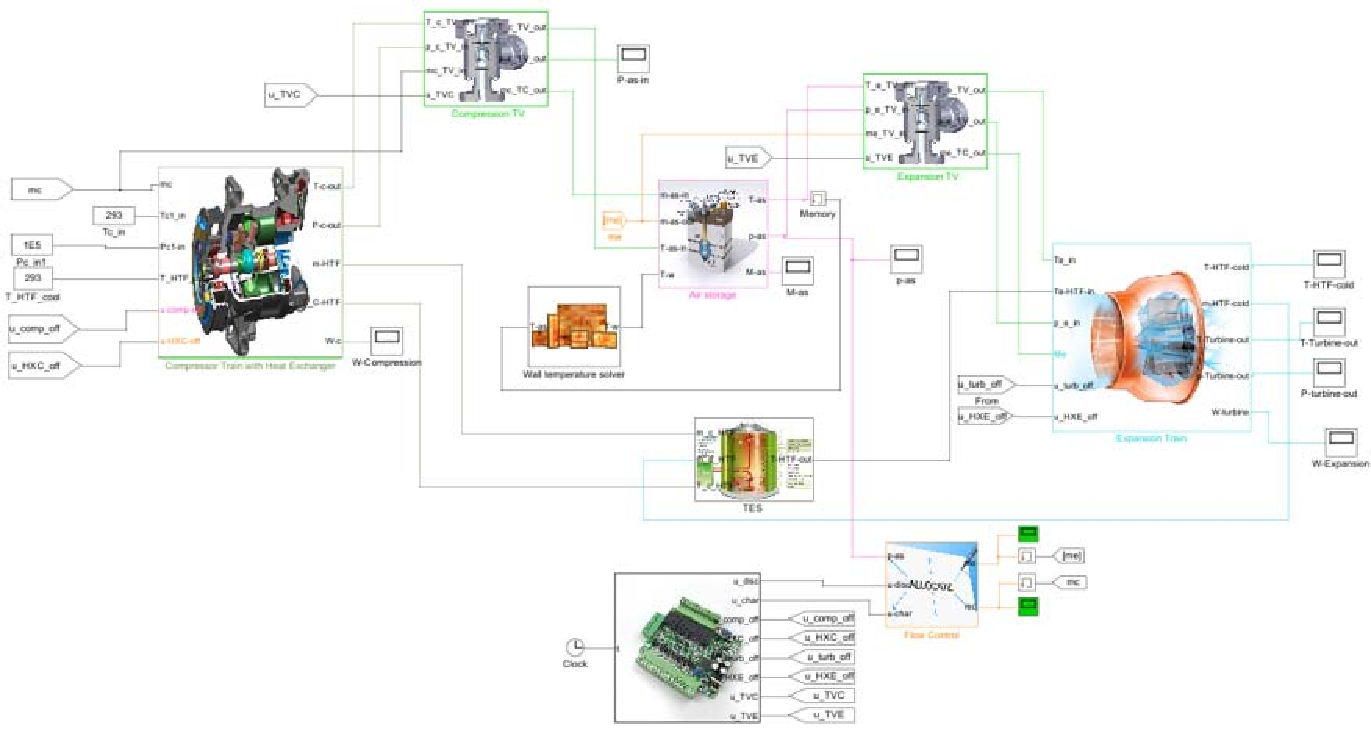
\includegraphics[scale=0.70]{Chap2-X-Simulation-Platform.pdf}
  \caption{计及组件部分负载特性的AA-CAES宽工况热力学仿真系统}
  \label{fig:Simulation-Platform}
\end{figure}

需要说明的是,目前存在可进行AA-CAES热力学特性仿真的软件,如Thermoflex 等,但其只能进行系统在任一给定运行点的性能,难以给出整个系统运行过程中的动态特性(储热系统、储气库),从而不便于分析一个循环周期内AA-CAES内部热力学参数间的相互耦合关系,同时也难以给出AA-CAES的宽工况运行特性。

\subsection{典型系统设计参数}
图\ref{fig:CAES-thermal-struc}给出了两级压缩两级膨胀的AA-CAES结构,尽管如此,本章的分析方法适用于任何多级压缩多级膨胀的AA-CAES系统的稳态热力学特性分析。本节基于所建的热力学稳态仿真模型分析一典型的小型AA-CAES系统的运行特性,该系统中的压缩机、膨胀机、换热器等组件的热力学设计参数分别见表
\ref{tab:TICC-500-para-comp} 至表\ref{tab:TICC-500-para-he-turb},相关数据基于文献~\inlinecite{Thesis-Wangsixian,Thesis-Zhangxuelin}改编而来。

我们假定采用文献\inlinecite{TICC-15}中的五级压缩三级膨胀结构,储气库无入口侧节流阀,但有出口侧节流阀,即AA-CAES运行于滑压-定压模式。同时,系统采用加压水作为HTF,相应的储热系统采用低温双罐储热结构。

%该系统参数常被用于AA-CAES相关研究的基准数据,如文献~\inlinecite{Variable-Conf-18,TICC-16}。

\begin{table}[htb]
  \centering
  \begin{minipage}[t]{0.79\linewidth} % 如果想在表格中使用脚注,minipage是个不错的办法
  \caption{压缩机额定参数}
  \label{tab:TICC-500-para-comp}
    \begin{tabularx}{\linewidth}{ccccccc}
      \toprule[1.5pt]
      {\heiti 级数} &  {\heiti $\beta_c$} & {\heiti $\eta_c$ (\%)} &  {\heiti $p_c^{in}$ (MPa)} & {\heiti $p_c^{out}$ (MPa)} & {\heiti $T_c^{in}$ ($^{\circ}$C)} & {\heiti $T_c^{out}$ ($^{\circ}$C)}\\
     \midrule[1pt]
      一级 & 3.5   & 74.4 & 0.1 & 0.35   & 25 & 153 \\
      二级 & 2.676 & 77.5 & 0.34 & 0.91  & 45 & 146.7 \\
      三级 & 2.697 & 80.5 & 0.89 & 2.40  & 45 & 147.6 \\
      四级 & 2.468 & 82.4 & 2.35 & 5.80  & 45 & 142.2 \\
      五级 & 1.963 & 83.0 & 5.72 & 11.23 & 45 & 109.1 \\
      \bottomrule[1.5pt]
    \end{tabularx}
  \end{minipage}
\end{table}

\begin{table}[htb]
  \centering
  \begin{minipage}[t]{0.79\linewidth} % 如果想在表格中使用脚注,minipage是个不错的办法
  \caption{膨胀机额定参数}
  \label{tab:TICC-500-para-turb}
    \begin{tabularx}{\linewidth}{ccccccc}
      \toprule[1.5pt]
      {\heiti 级数} & {\heiti $\beta_e$} &  {\heiti $\eta_e$ (\%)} & {\heiti $p_e^{in}$ (MPa)} & {\heiti $p_e^{out}$ (MPa)} & {\heiti $T_e^{in}$ ($^{\circ}$C)} &{\heiti $T_e^{out}$ ($^{\circ}$C)} \\
     \midrule[1pt]
      一级 & 2.212 & 82.6 & 2.50 & 1.13  & 100 & 12 \\
      二级 & 2.8 & 81.0 & 1.12 & 0.40  & 100 & 13 \\
      三级 & 3.714 & 81.6 & 0.39 & 0.105 & 100 & 13 \\
      \bottomrule[1.5pt]
    \end{tabularx}
  \end{minipage}
\end{table}

\begin{table}[htb]
  \centering
  \begin{minipage}[t]{0.88\linewidth} % 如果想在表格中使用脚注,minipage是个不错的办法
  \caption{压缩侧换热器额定参数}
  \label{tab:TICC-500-para-he-comp}
    \begin{tabularx}{\linewidth}{cccccc}
      \toprule[1.5pt]
      {\heiti 级数} & {\heiti $T_{c,HX}^{a,in}$ ($^{\circ}$C)} & {\heiti $T_{c,HX}^{a,out}$ ($^{\circ}$C)} & {\heiti $T_{c,HX}^{HTF,in}$ ($^{\circ}$C)} & {\heiti $T_{c,HX}^{HTF,out}$ ($^{\circ}$C)}&{\heiti $\dot m_{c,HX}^{HTF}$ (kg/s)}\\
     \midrule[1pt]
      一级 & 153   & 45 & 35 & 120  & 0.1346 \\
      二级 & 146.7 & 45 & 35 & 120  & 0.1268 \\
      三级 & 147.6 & 45 & 35 & 120  & 0.1279 \\
      四级 & 142.2 & 45 & 35 & 120  & 0.1212 \\
      五级 & 109.1 & 45 & 35 & 60   & 0.2755 \\
      \bottomrule[1.5pt]
    \end{tabularx}
  \end{minipage}
\end{table}

\begin{table}[htb]
  \centering
  \begin{minipage}[t]{0.89\linewidth} % 如果想在表格中使用脚注,minipage是个不错的办法
  \caption{膨胀侧换热器额定参数}
  \label{tab:TICC-500-para-he-turb}
    \begin{tabularx}{\linewidth}{cccccc}
      \toprule[1.5pt]
      {\heiti 级数} & {\heiti $T_{e,HX}^{a,in}$ ($^{\circ}$C)} & {\heiti $T_{e,HX}^{a,out}$ ($^{\circ}$C)} & {\heiti $T_{e,HX}^{HTF,in}$ ($^{\circ}$C)} & {\heiti $T_{e,HX}^{HTF,out}$ ($^{\circ}$C)} & {\heiti $\dot m_{e,HX}^{HTF}$ (kg/s)}\\
     \midrule[1pt]
      一级 & -15 & 100 & 120 & 35  & 0.7855\\
      二级 & 30  & 100 & 120 & 35  & 0.5936\\
      三级 & 25  & 100 & 120 & 35  & 0.5943\\
      \bottomrule[1.5pt]
    \end{tabularx}
  \end{minipage}
\end{table}

\subsection{设计工况性能}
\label{sec:chap2-model-valid-Thermoflex}
额定设计点的运行性能分析旨在说明AA-CAES内部各组件运行特性之间的相互影响,我们重点分析AA-CAES在滑压-定压运行模式下能量转换类组件(压缩机、膨胀机)及能量转移类组件(换热器)的运行特性与能量存储类组件(储气库及储热罐)的动态特性之间的耦合关系。

\subsubsection{压缩储能过程}
我们设定储气库的运行压力范围为4MPa-10MPa,储气库的体积取为100 m$^2$(与文献\inlinecite{TICC-15}中的实际电站一致)。压缩储能过程以压缩机的额定质量流率(0.4492kg/s)进行压缩储能,在给定的压缩侧滑压运行模式下,压缩储能过程的总时间为2.9h,各级压缩机的出口空气压力的变化过程如图
\ref{fig:Sim-Char-Inlet-Pressure}所示。

\begin{figure}[H] % use float package if you want it here
  \centering
  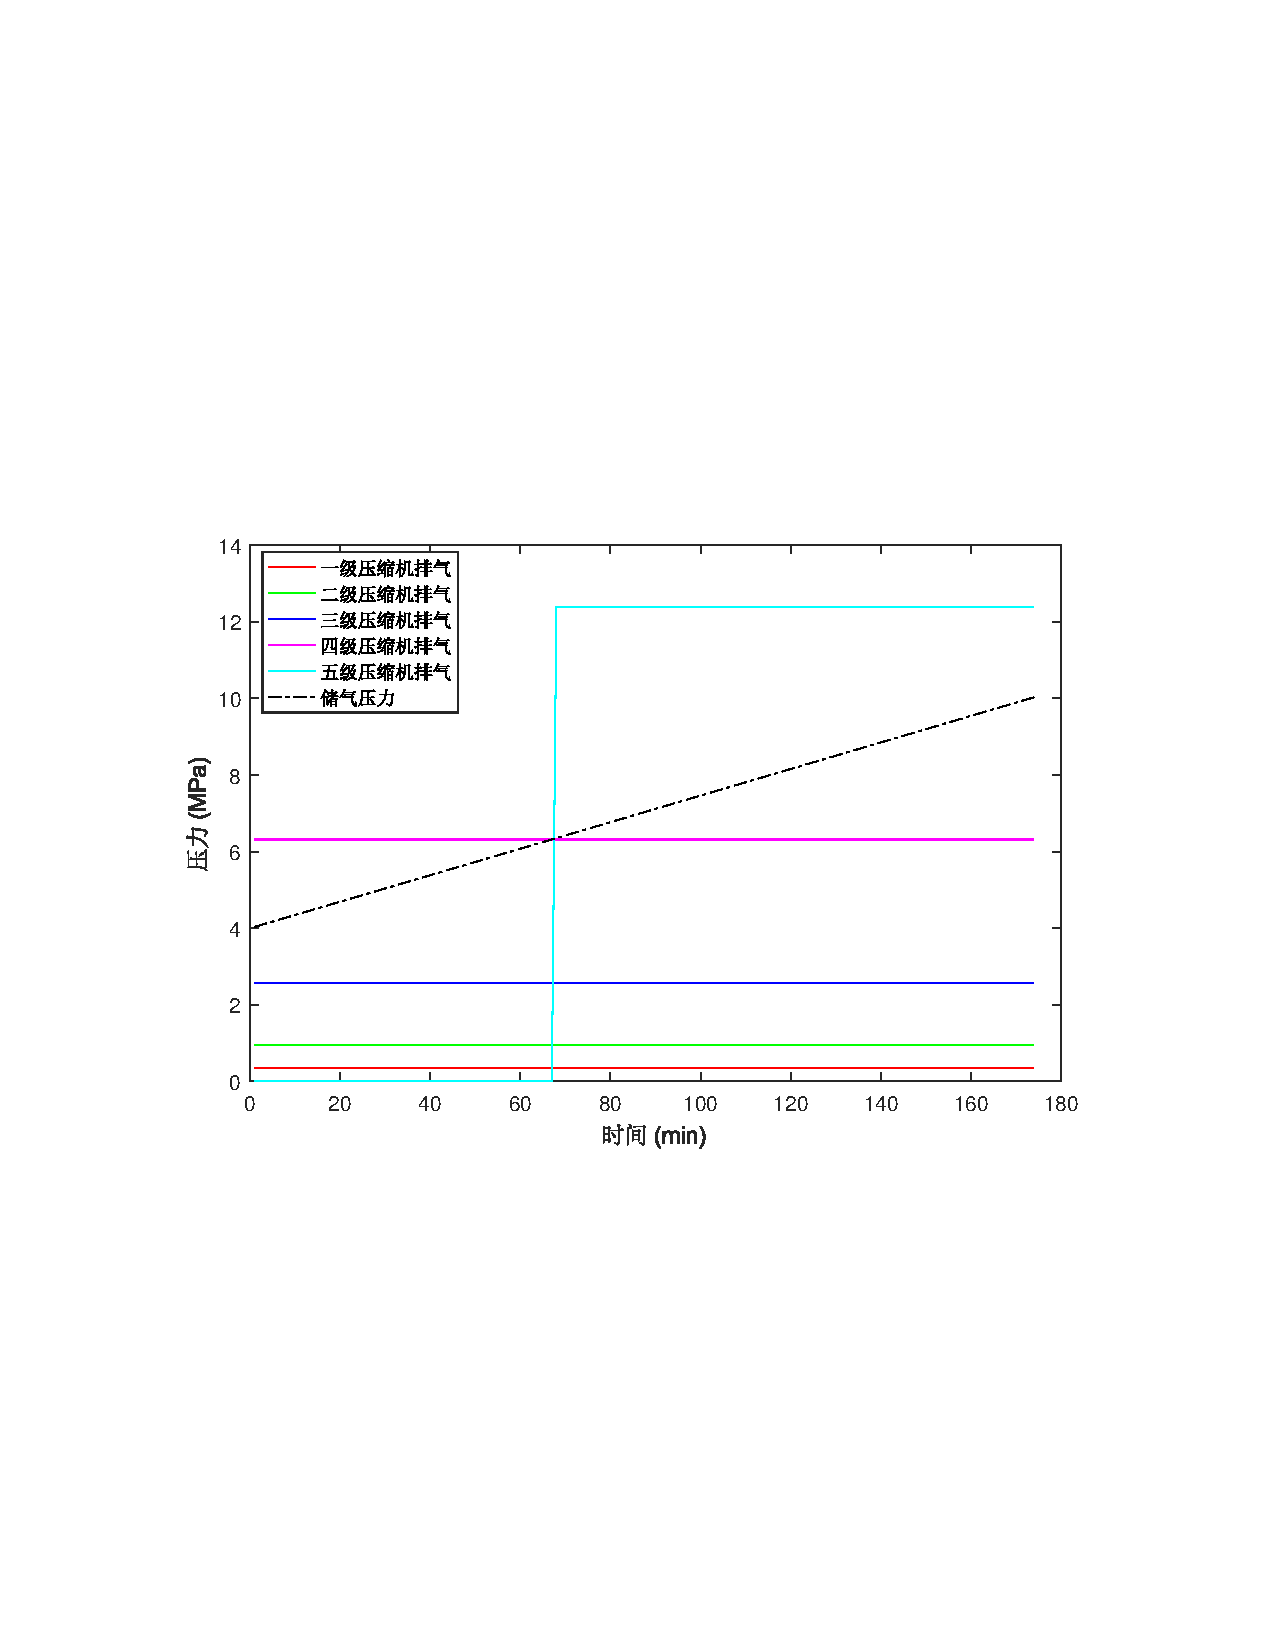
\includegraphics[scale=0.70]{Chap2-Sim-Char-Inlet-Pressure.pdf}
  \caption{压缩储能过程各级压缩机出口压力变化曲线(设计工况)}
  \label{fig:Sim-Char-Inlet-Pressure}
\end{figure}

由于压缩侧采用了滑压运行模式,压缩机将承受储气库背压,而随着储能过程的进行,储气库压力升高,压缩机承受的背压也将增大,各级压缩机的运行状态也有所不同。压缩初始状态,储气库压力为4MPa,需要启动前四级压缩机;随着储气库空气压力增至6.2MPa(第65min),第5级压缩机启动,从而将末级压缩机的出口空气压力提升至10MPa以上,以克服储气库的实时压力进行储气。此外,由于我们设定不考虑换热器的压损特性,导致每级压缩机的排气压力略高于额定排气压力。

对于小型AA-CAES,由于储气库体积较小,容易实现绝热储气,我们采用了VA模型。在储能过程中储气库中空气的热力学动态如图\ref{fig:Sim-Char-ASU-P-M}所示。在VA模型的设定下,储气库不与外界进行换热,随着高压空气(高温)的注入,储气库内空气的质量、温度及压力均上升。为了维持储气库的最低运行压力,储气库在初始状态需存储一定的空气,由理想气体状态方程可得初始空气质量为4.7617$\times10^3$ kg/,由于以额定质量流率储气,储气库中空气质量线性增长。

\begin{figure}[H] % use float package if you want it here
  \centering
  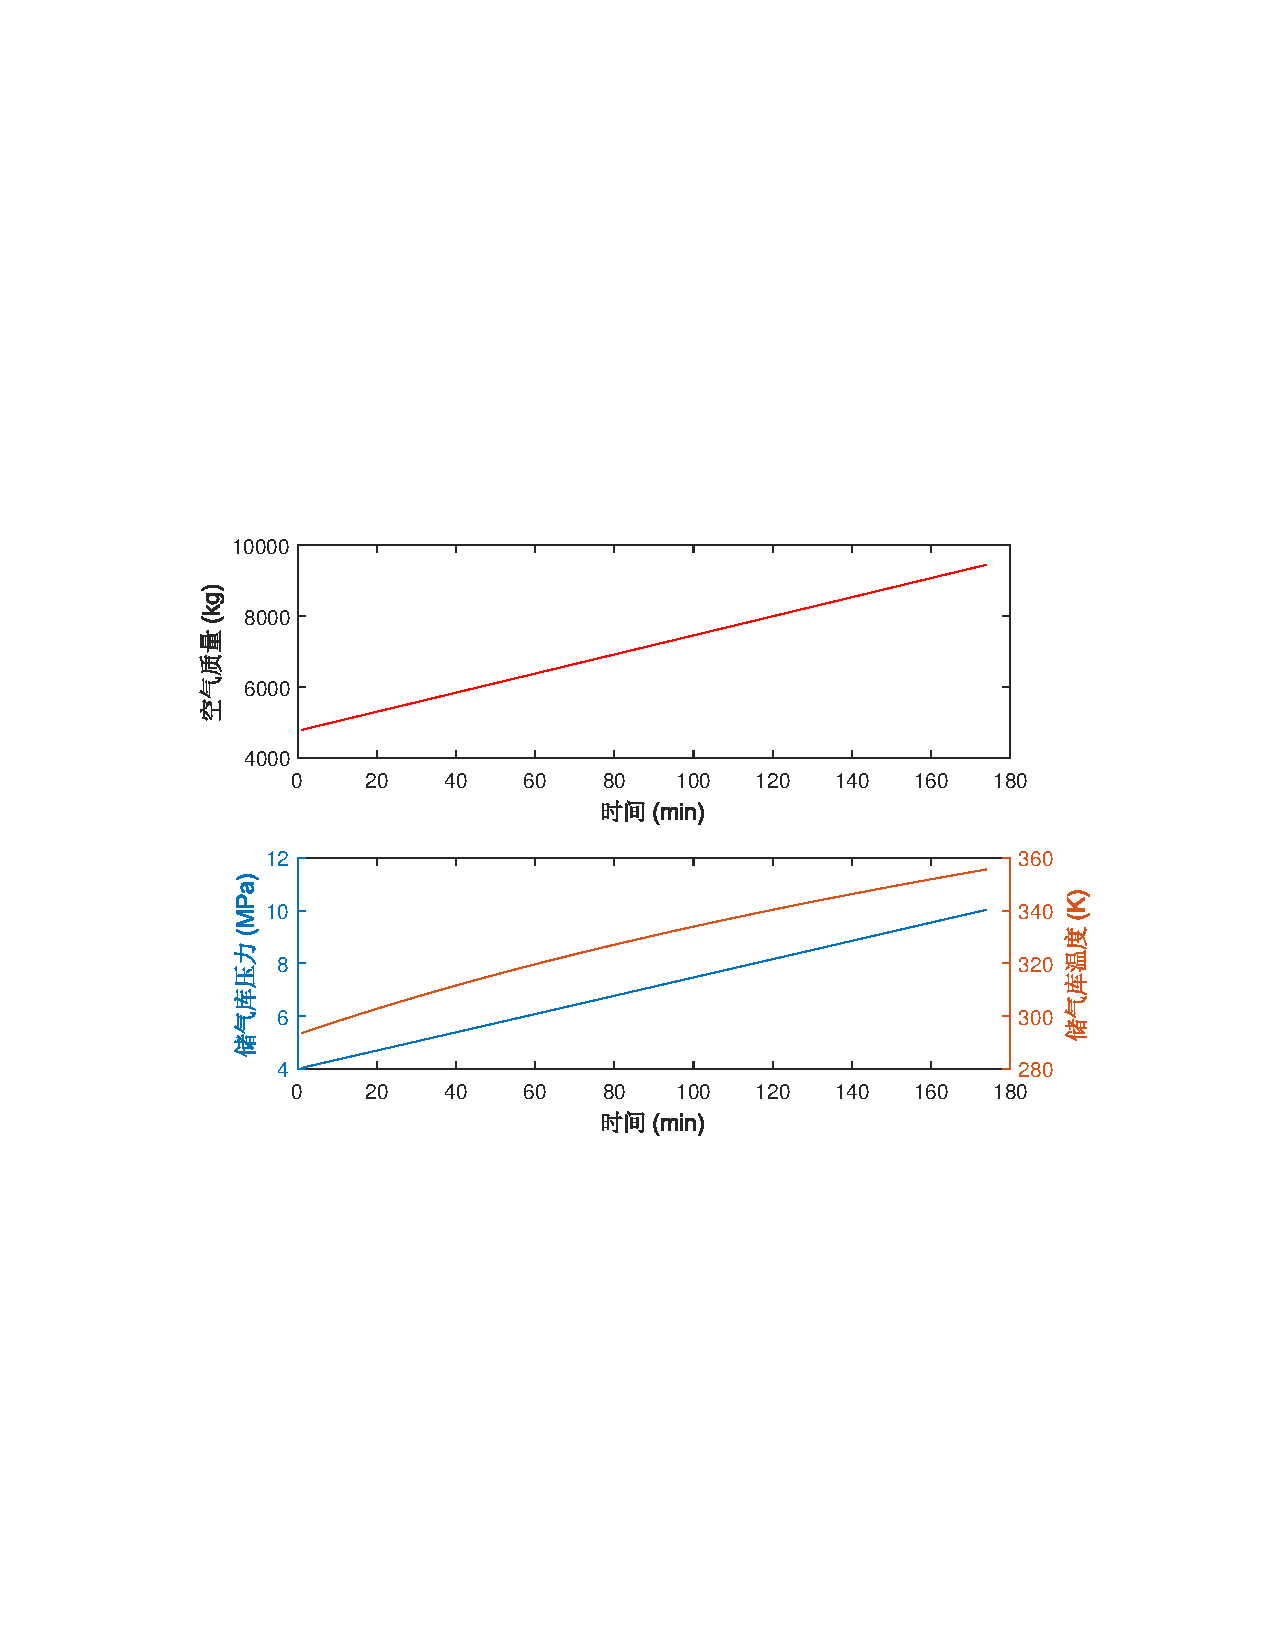
\includegraphics[scale=0.75]{Chap2-Sim-Char-ASU-P-M.pdf}
  \caption{压缩储能过程储气库动态特性(设计工况)}
  \label{fig:Sim-Char-ASU-P-M}
\end{figure}

在第5级压缩机未启动前,储气库进口空气的热力学参数由第4级换热器出口空气决定,当第5级压缩机启动后则由第5级换热器出口空气的热力学参数决定。因此,储气库的压力呈现两段线性增长趋势,而温度与储气库中空气的实时质量有关,并不线性增长。

\begin{figure}[H] % use float package if you want it here
  \centering
  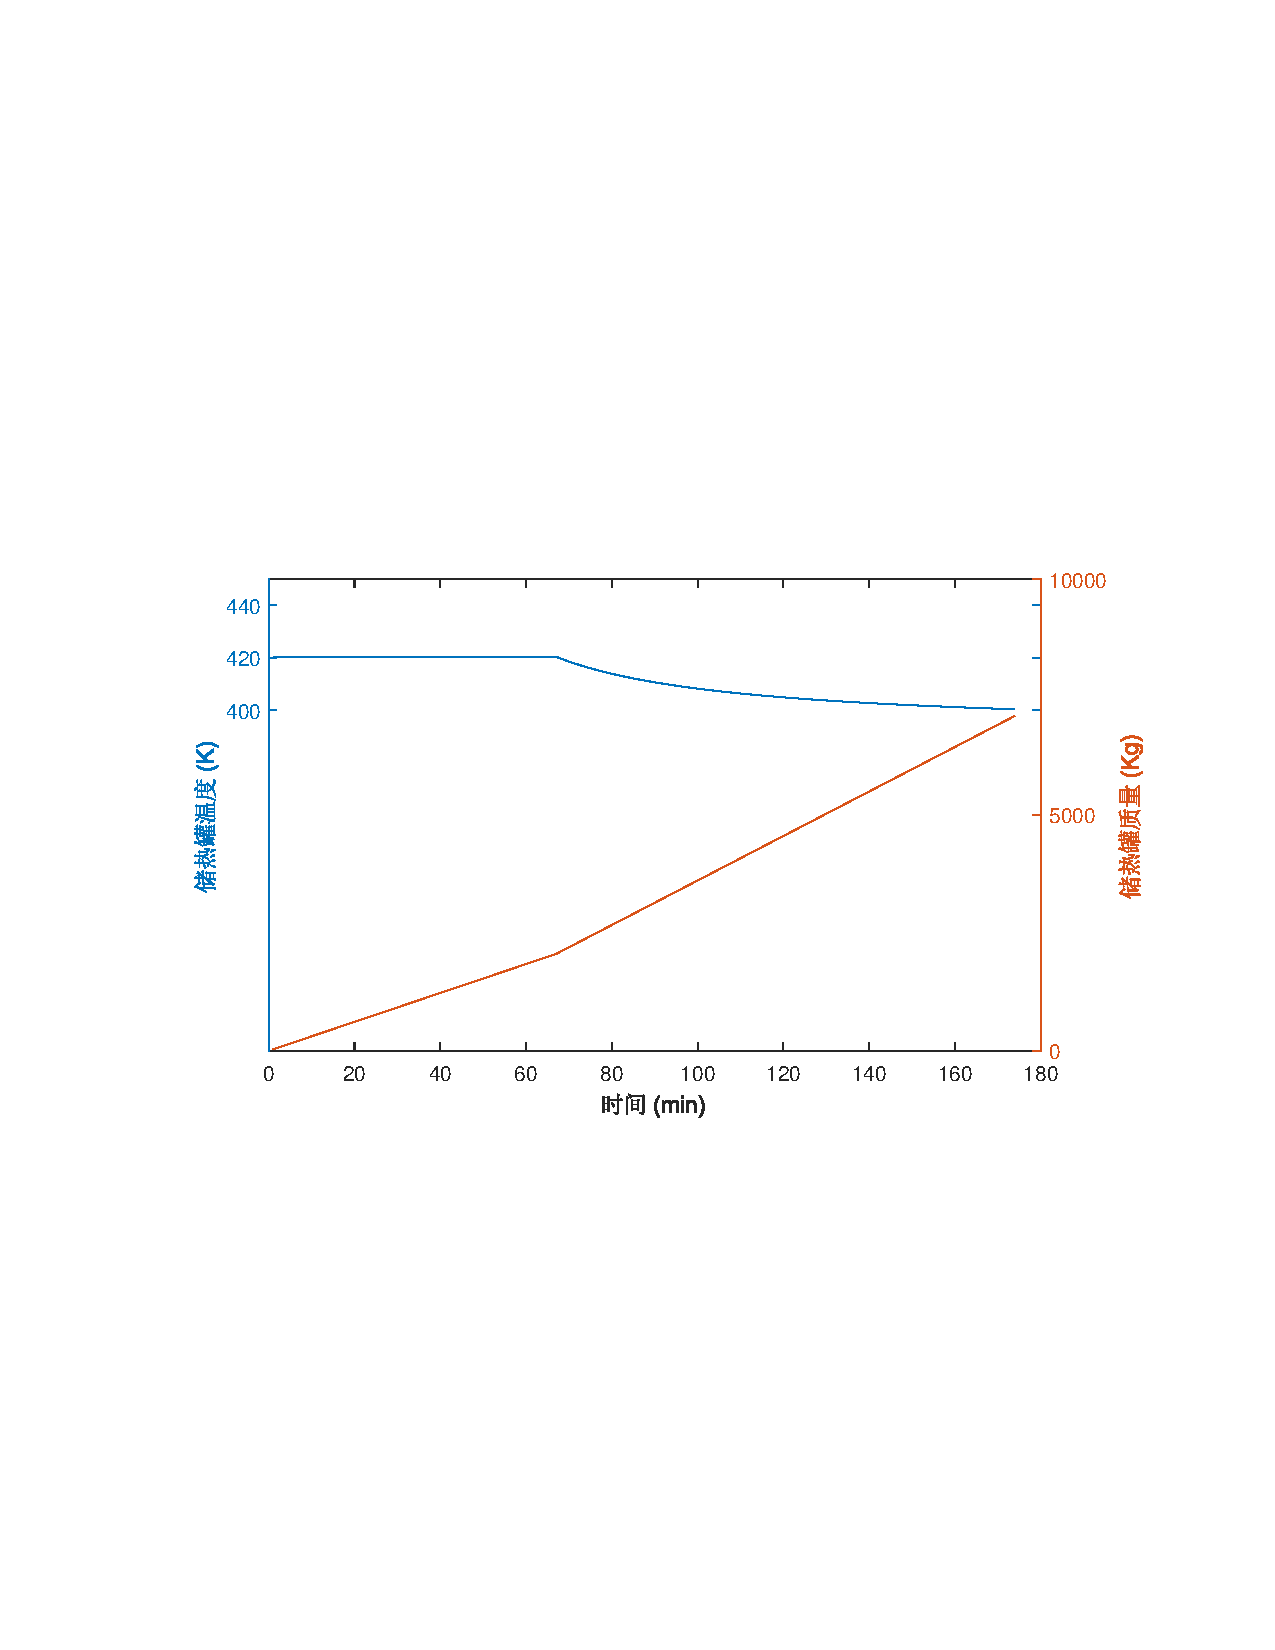
\includegraphics[scale=0.70]{Chap2-Sim-Char-TES.pdf}
  \caption{压缩储能过程储热罐动态特性(设计工况)}
  \label{fig:Sim-Char-TES}
\end{figure}

小容量储热系统容易实现绝热模型,我们假定系统在储能初始状态下高温储热罐中HTF的质量为0,压缩储能过程中高温储热罐的HTF的热力学动态特性如图
\ref{fig:Sim-Char-TES}所示。在第5级压缩机未启动之前,由于以额定质量流率压缩,HTF侧也以固定的质量流率进行储热(一般维持换热器的热容比$C_{c,HX}$为定值),储热罐中的HTF质量增大。第5级压缩机启动后,注入储热罐中的HTF质量流率将进一步增大,从而增大了储热罐中HTF 质量变化的斜率。同时,由于前五级换热器的HTF汇合温度(392.12K)低于前四级换热器的HTF汇合温度(420.30K),导致储热罐中HTF的温度从第56min起先下降(根据温度混合方程),随着储热过程的结束,HTF的温度渐渐平稳。储热过程结束时,储热罐中的HTF总质量为7.0973$\times 10^3$ kg,HTF的温度为400.27K。

在设计工况下,压缩侧各级换热器的换热功率及各级压缩机的耗功变化曲线分别如图\ref{fig:Sim-Char-Heat-Quan}及图\ref{fig:Sim-Char-Comp-Power}所示。由于我们假定AA-CAES 内部各组件在设计质量流率下以额定等熵效率运行,因此各级换热器的换热器量均为设计值,换热器运行于额定等熵效率。尽管各级换热器的HTF侧进口温度均为308.15K,但由于各级的热容比以及入口空气温度的差异,其换热功率不同。
\begin{figure}[H] % use float package if you want it here
  \centering
  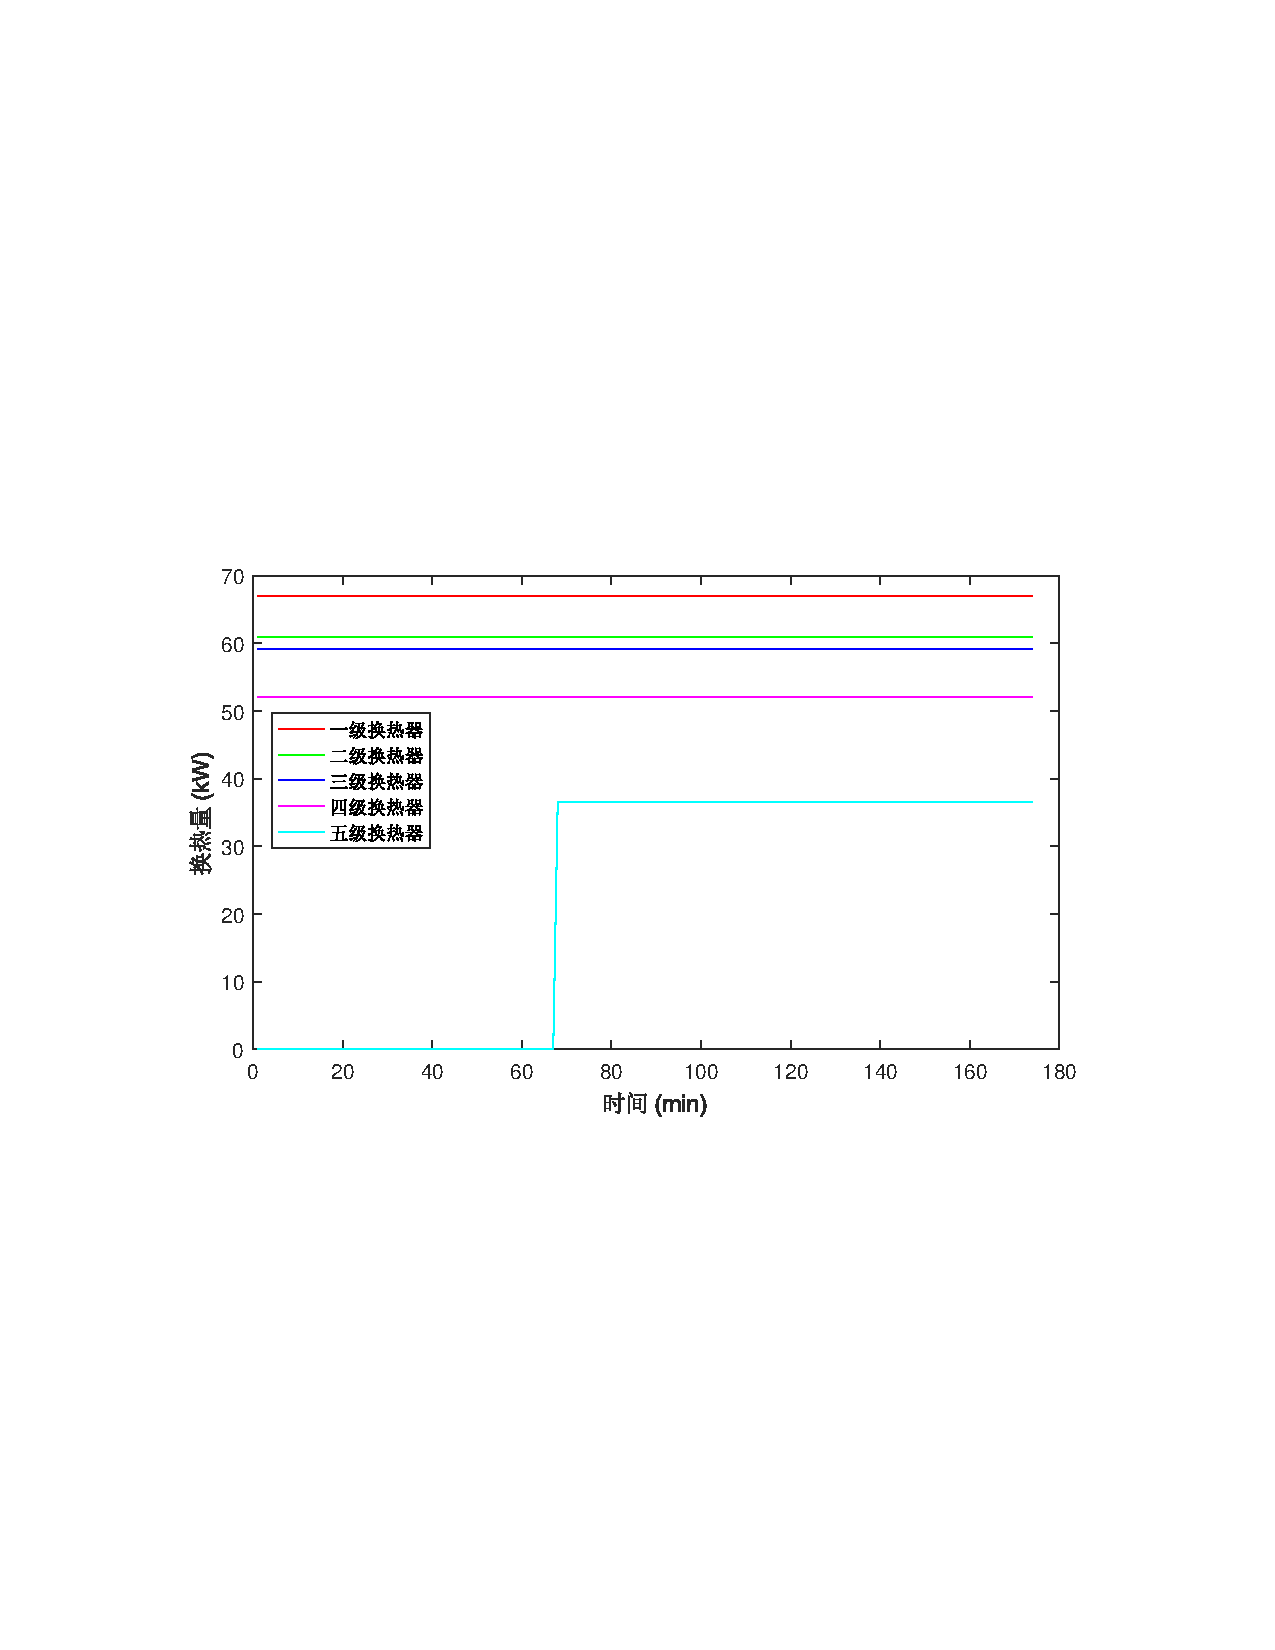
\includegraphics[scale=0.66]{Chap2-Sim-Char-Heat-Quan.pdf}
  \caption{压缩储能过程换热器换热功率变化曲线(设计工况)}
  \label{fig:Sim-Char-Heat-Quan}
\end{figure}

同时,在第5级压缩机未启动前,第1级至第4级压缩机消耗的额定电功率分别为77.73 kW,60.79 kW,58.98 kW,51.69 kW,系统总耗功为249.21kW;第5级压缩机启动后并消耗电功率36.93kW,从而将储能过程消耗的电功率提升至286.14kW。因此,我们不难发现,在压缩侧的滑压运行模式下,整个压缩储能过程不能一直实现满压缩功率储能,但各级压缩机可运行在额定设计工况。

\begin{figure}[H] % use float package if you want it here
  \centering
  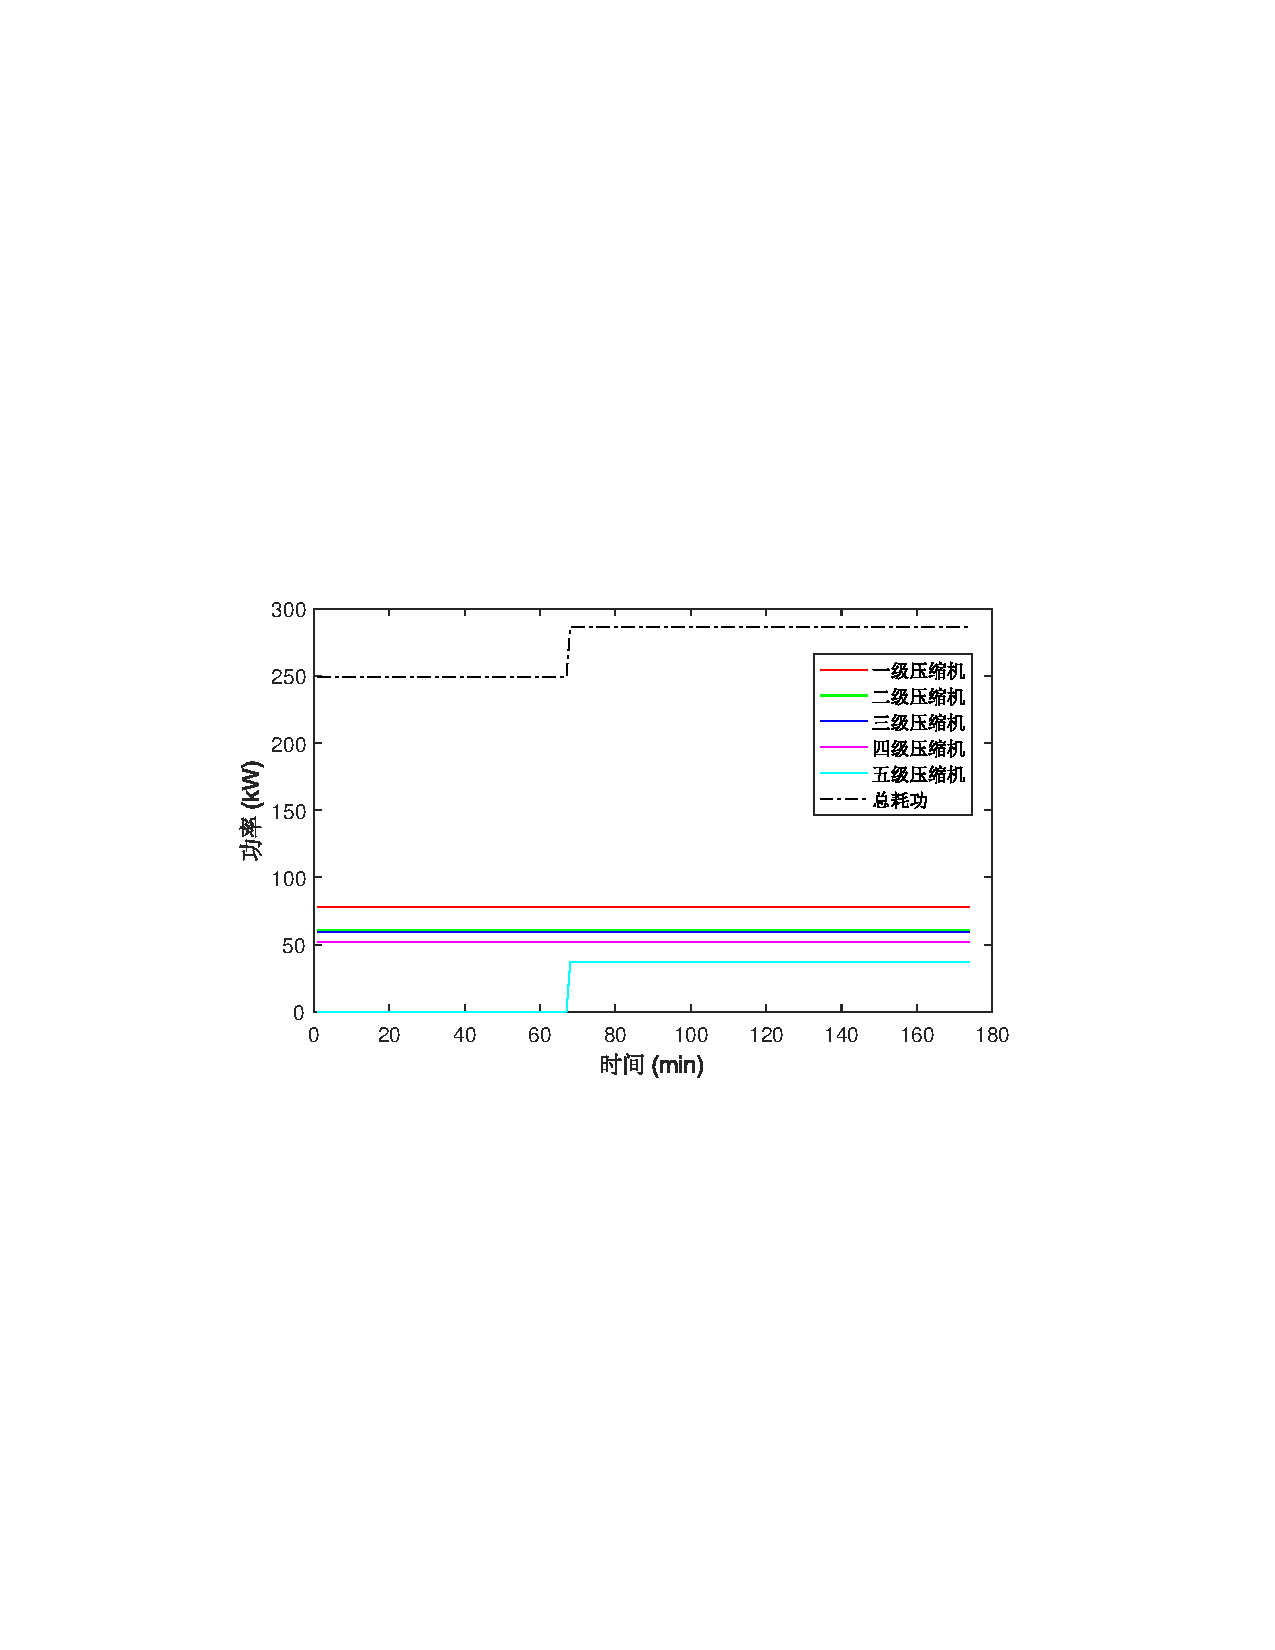
\includegraphics[scale=0.76]{Chap2-Sim-Char-Comp-Power.pdf}
  \caption{压缩储能过程压缩机耗功变化曲线(设计工况)}
  \label{fig:Sim-Char-Comp-Power}
\end{figure}
%需要说明的是,就整个AA-CAES对外特性而言,压缩侧处于滑压运行模式时

\subsubsection{膨胀释能过程}
与压缩储能过程类似,我们以膨胀机的额定质量流率(2.4435kg/s)进行膨胀释能,在给定的膨胀侧定压运行模式下,储气库的热力学动态特性如图
\ref{fig:Sim-Disc-ASU-P-T-M}所示,总释能时间为0.53h。由于采用了定压运行模式,第1级透平的进气压力为储气库的最低运行压力,即4MPa,随着释能过程的进行,储气库中空气的压力逐渐从压缩储能末端时的储气压力10MPa 逐渐减小,当储气压力减至储气库的最低运行压力时,释能过程结束。储气库内空气质量线性减少,而压力与温度并不呈线性趋势,其原因在于储气压力不仅与质量流率有关,还与储气库内空气的温度有关,而空气温度与时变的储气库空气质量有关。

\begin{figure}[H] % use float package if you want it here
  \centering
  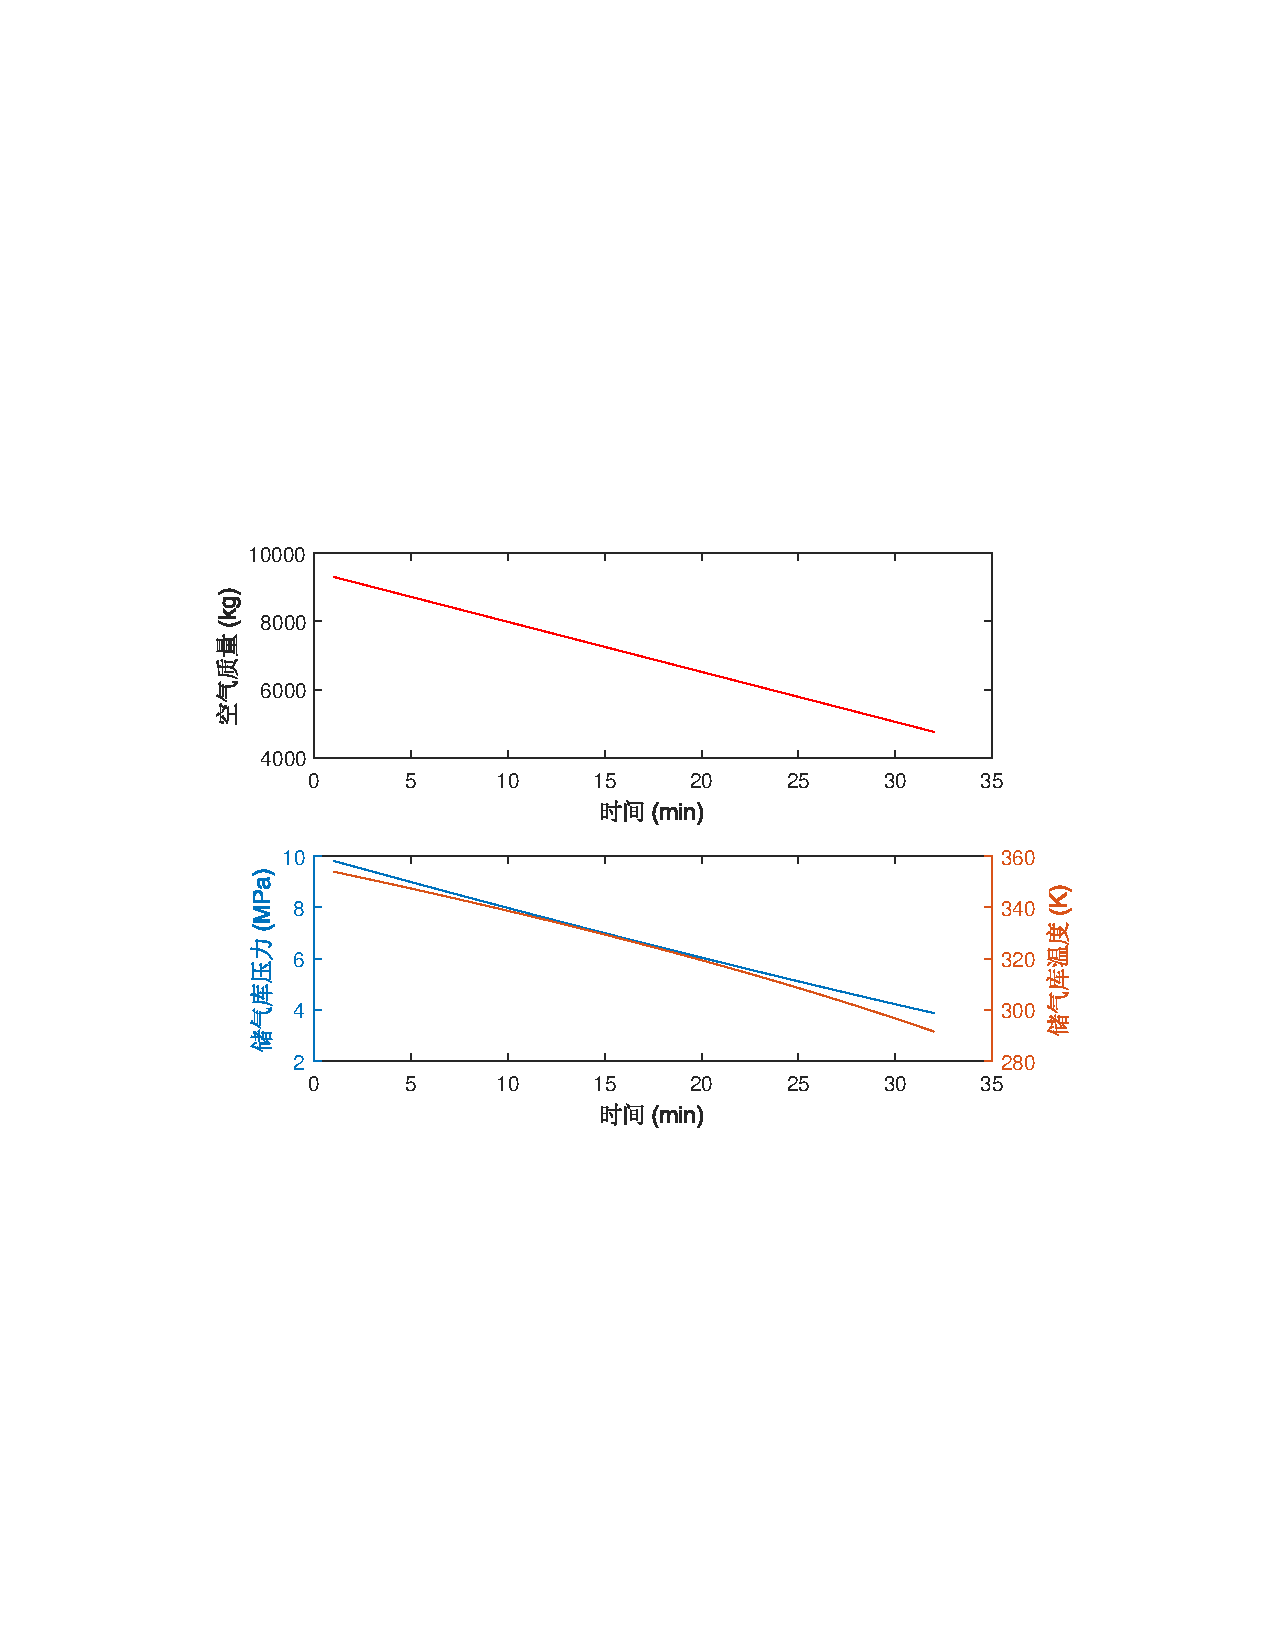
\includegraphics[scale=0.74]{Chap2-Sim-Disc-ASU-P-T-M.pdf}
  \caption{膨胀释能过程储气库动态特性(设计工况)}
  \label{fig:Sim-Disc-ASU-P-T-M}
\end{figure}

在储气库VA模型下,随着储气库中空气质量的减少,储气库中空气温度也持续下降,从释能开始时的355.58 K降至释能结束时的291.47K,进而逐渐增大了对
膨胀释能阶段各级换热器的换热功率需求。由图\ref{fig:Sim-Disc-Heat-Quan}所示的换热器换热功率变化曲线可以看出,1级换热器换热功率需求的变化最明显,从膨胀释能初始时的93.35kW,逐渐增至释能终止时的221.9kW,变化幅度达137.71\%;2级换热器换热功率的变化范围较小,从释能开始时的138.49kW增至释能结束时的152.94kW,增幅为10.43\%;3级换热器的换热功率基本维持不变。由此可以得出,随着释能过程的进行,越靠近储气库的换热器换热功率的变化越大,而后级换热器换热功率的变化越来越小,其主要原因在于通过前级换热器的“缓冲”,后级换热器的进口空气温度在释能过程中可以维持在较小的变化范围。

\begin{figure}[H] % use float package if you want it here
  \centering
  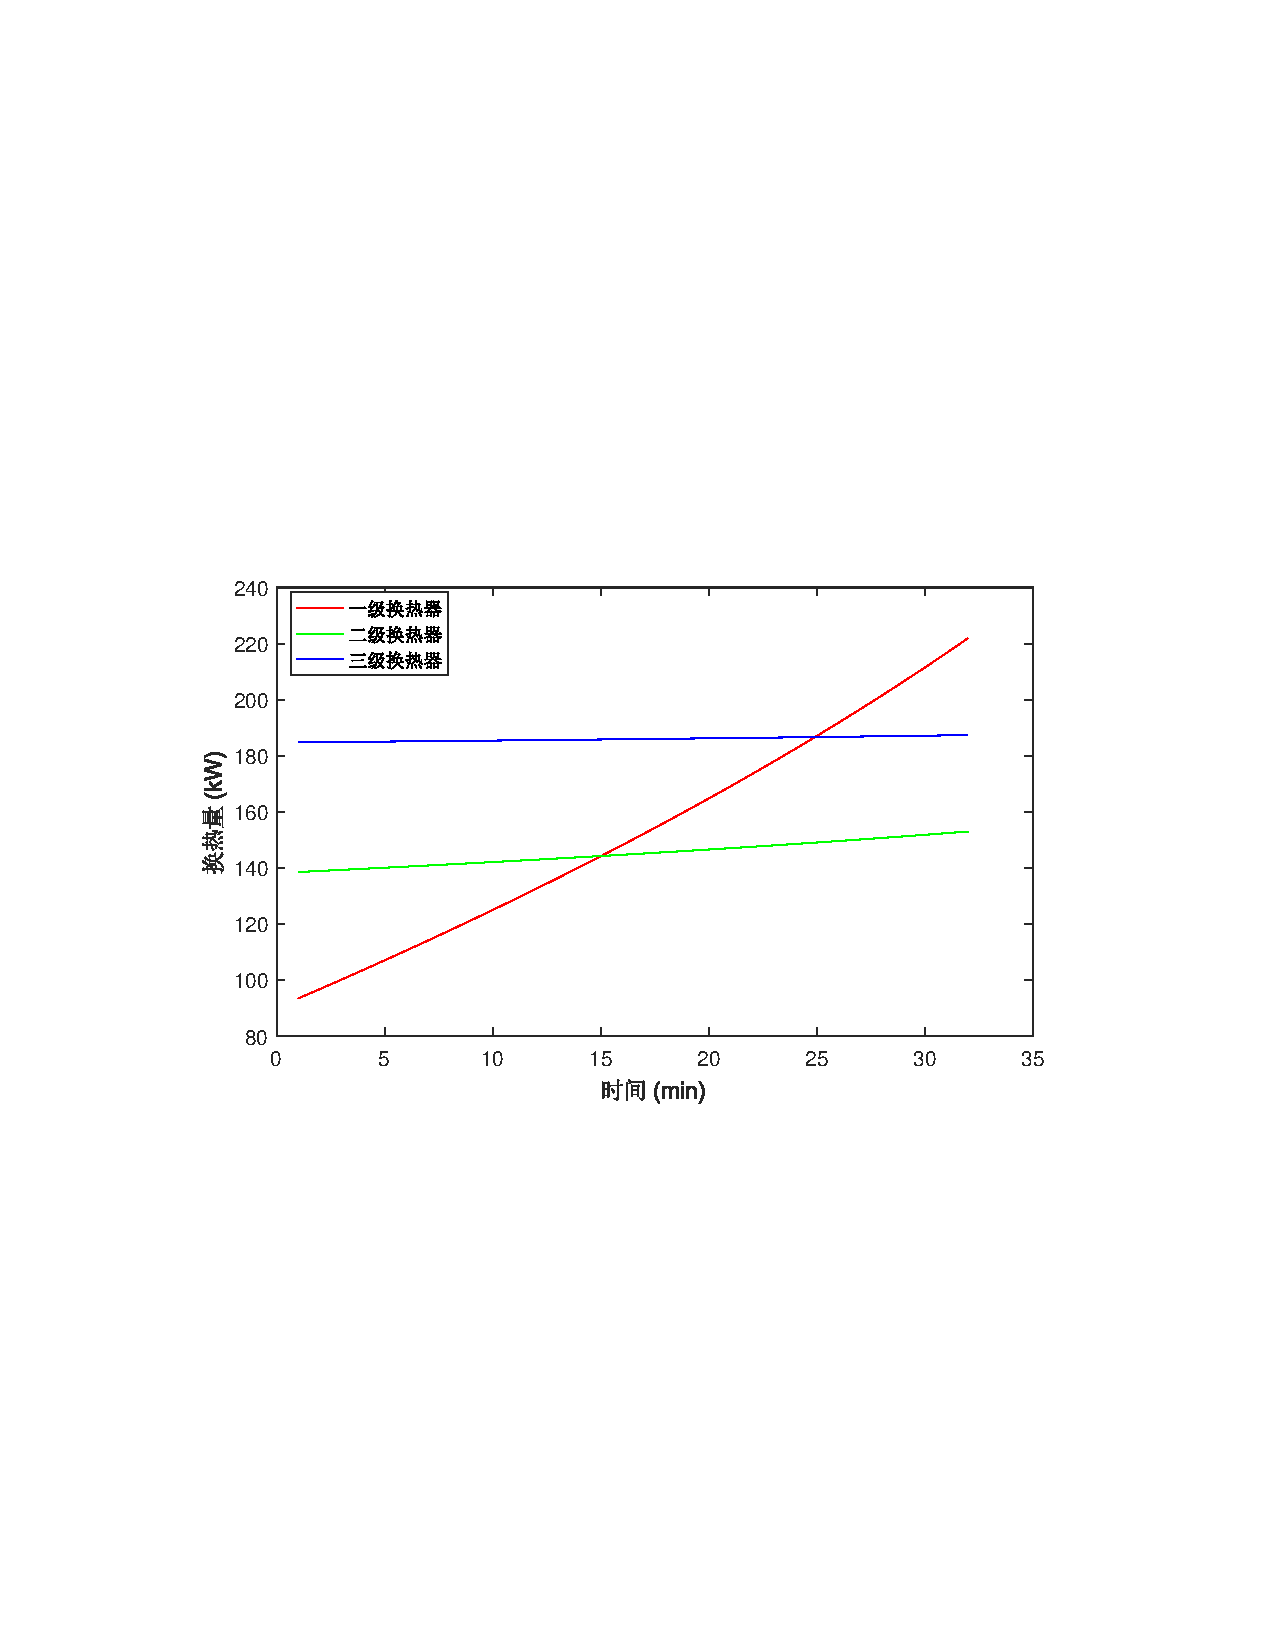
\includegraphics[scale=0.75]{Chap2-Sim-Disc-Heat-Quan.pdf}
  \caption{膨胀释能过程换热器换热功率(设计工况)}
  \label{fig:Sim-Disc-Heat-Quan}
\end{figure}

与图\ref{fig:Sim-Disc-Heat-Quan}中换热器换热功率的变化一致,随着释能过程中储气库内空气压力及温度的降低,各级透平的输出功率也相应下降,但变化不大。图
\ref{fig:Sim-Disc-Turb-Power}给出了膨胀释能过程中第1级透平输出功率及AA-CAES系统的总膨胀功率的变化曲线。第1级透平的输出功率从161.8kW减至158.06kW,变化率为2.31\%,三级透平的总输出(电)功率从594.06kW减至589.29kW,变化仅为0.8\%。由此可见,通过换热器及储热系统的配合,让换热器承担(或缓解)储气库内空气温度的下降对释能过程的影响,即可在透平侧的定压运行模式下实现稳定的功率输出,可以说,这正是AA-CAES这一储能循环采用储气与储热实现“气热双储”带来的灵活性。

\begin{figure}[H] % use float package if you want it here
  \centering
  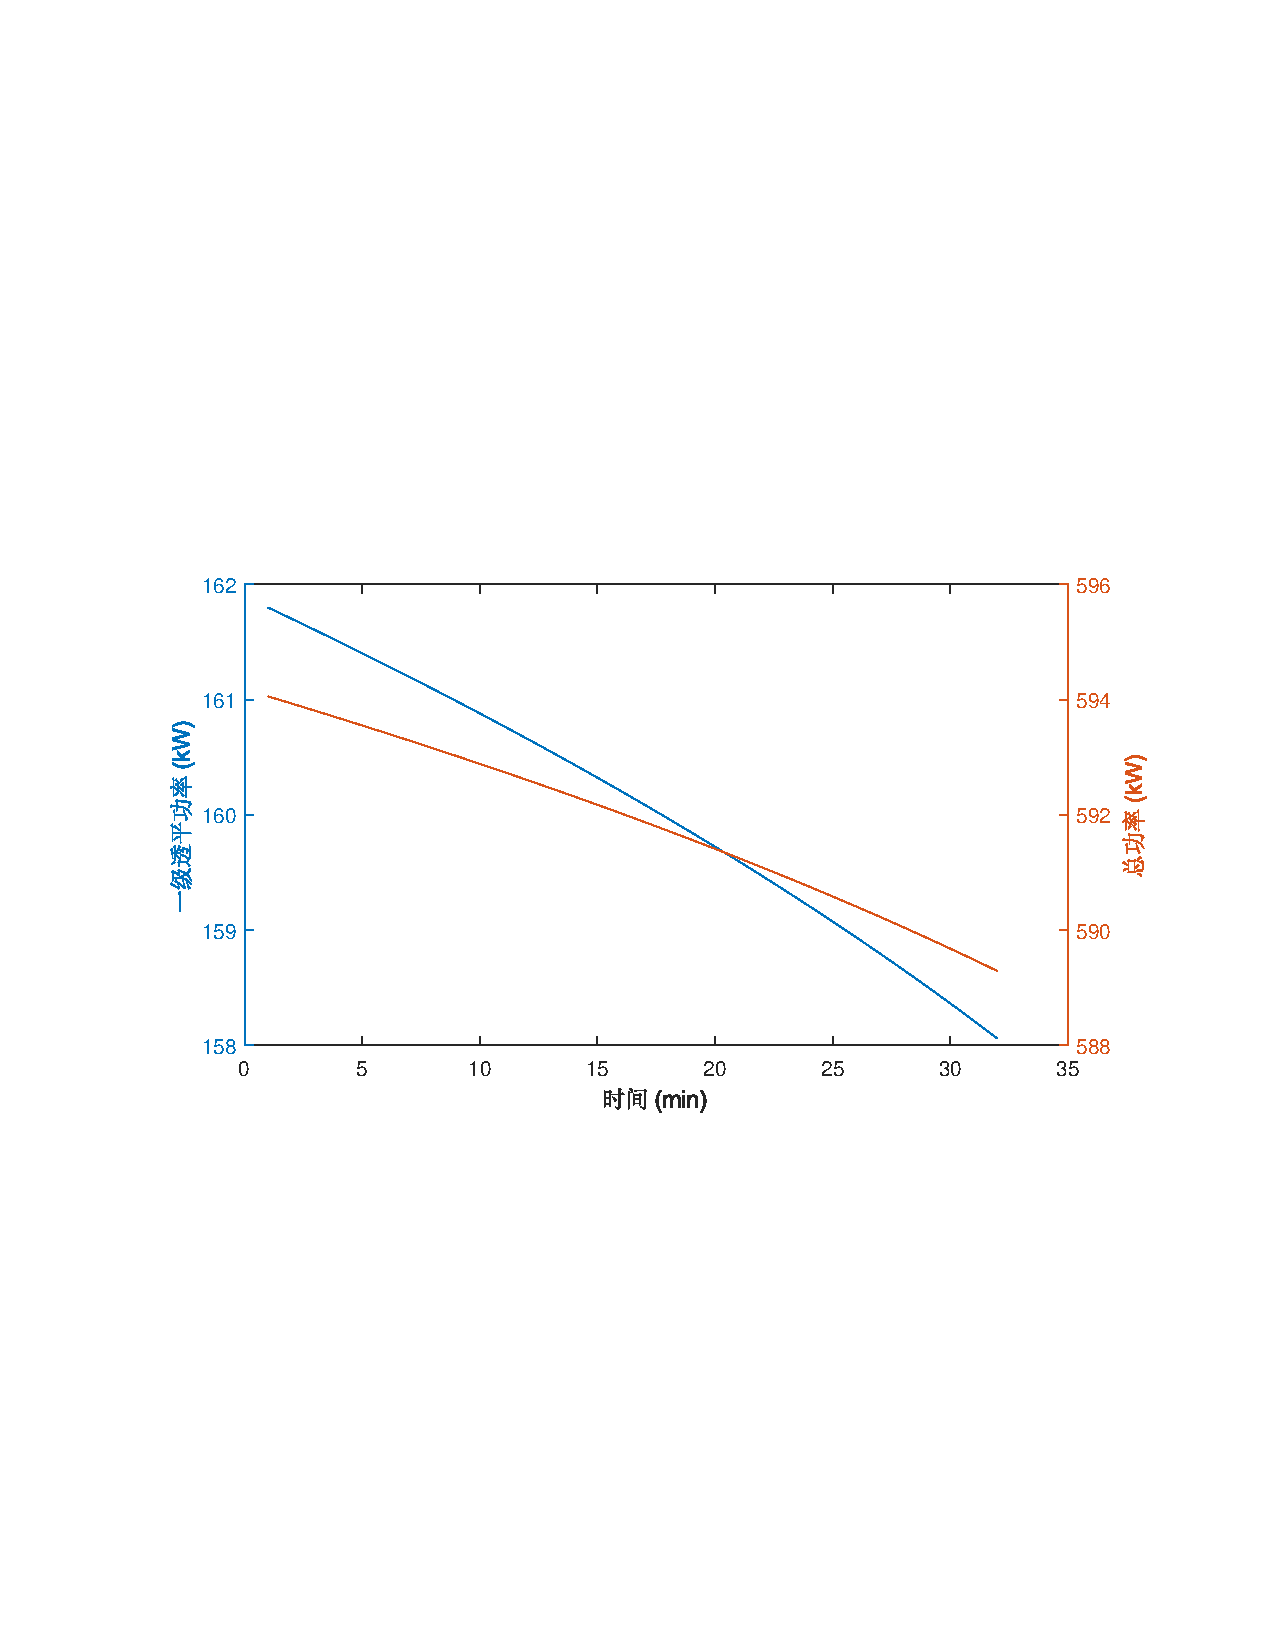
\includegraphics[scale=0.72]{Chap2-Sim-Disc-Turb-Power.pdf}
  \caption{膨胀释能过程输出功率变化曲线(设计工况)}
  \label{fig:Sim-Disc-Turb-Power}
\end{figure}

综上,在滑压-定压运行模式下,以额定质量流率进行储能与释能的一个循环周期中,AA-CAES消耗的总电量为0.7886MWh,输出的总电量为0.3157MWh,其电-电效率$\eta_{elec}$为40.03\%。 同时,储能结束时高温储热罐中的HTF质量为6.9784$\times 10^3$kg,释能结束时储热罐中剩余的高温HTF质量为3.2941$\times10^3$kg,温度为400.27K,该部分热水可用于供热,总供热量可达0.3524MWh,供热效率$\eta_{heat}$为44.69\%,系统热电联供的总能利用系数$\eta_{total}$为84.72\%。供热量的热量㶲为0.0944MWh,供热㶲效率$\eta_{x,heat}$为11.97\%,热电联供总㶲效率$\eta_{x,total}$为52\%。此外,尽管本文不关注制冷,但透平末级排气温度(283.01K)低于环境温度,该部分能量可用于制冷,进而AA-CAES多能联供的总能利用系数及㶲效率均可提高。事实上,图\ref{fig:Sim-Char-Inlet-Pressure}中第5级压缩机排气压力高于储气库的实时压力,存在一定的能量损失,若让第5级压缩机运行于一定的非设计工况,使得其排气压力与储气库压力一致,即可降低第5级压缩机的耗功,从而可进一步提升系统的各能效指标。

\subsection{部分负载性能}
\label{sec:chap2-model-valid-TICC}
实际运行过程中,除了内部组件之间的耦合关系之外,能量转换类组件(压缩机、膨胀机)及能量转移类组件(换热器)的部分负载运行特性对AA-CAES系统运行特性也有着重要的影响。特别是,当挖掘AA-CAES的容量备用等灵活性特性时,压缩储能过程中的质量流率与膨胀释能过程中的质量流率将偏离压缩机与膨胀机(及与之匹配的换热器)的额定质量流率,进而影响内部能量转换、能量转移及能量存储组件的热力学特性。我们以图\ref{fig:Sim-massflow-Part-load}所示的部分负载质量流率模拟电力系统对AA-CAES的宽工况运行要求,进而分析对应的压缩储能与膨胀释能过程。

\begin{figure}[H] % use float package if you want it here
  \centering
  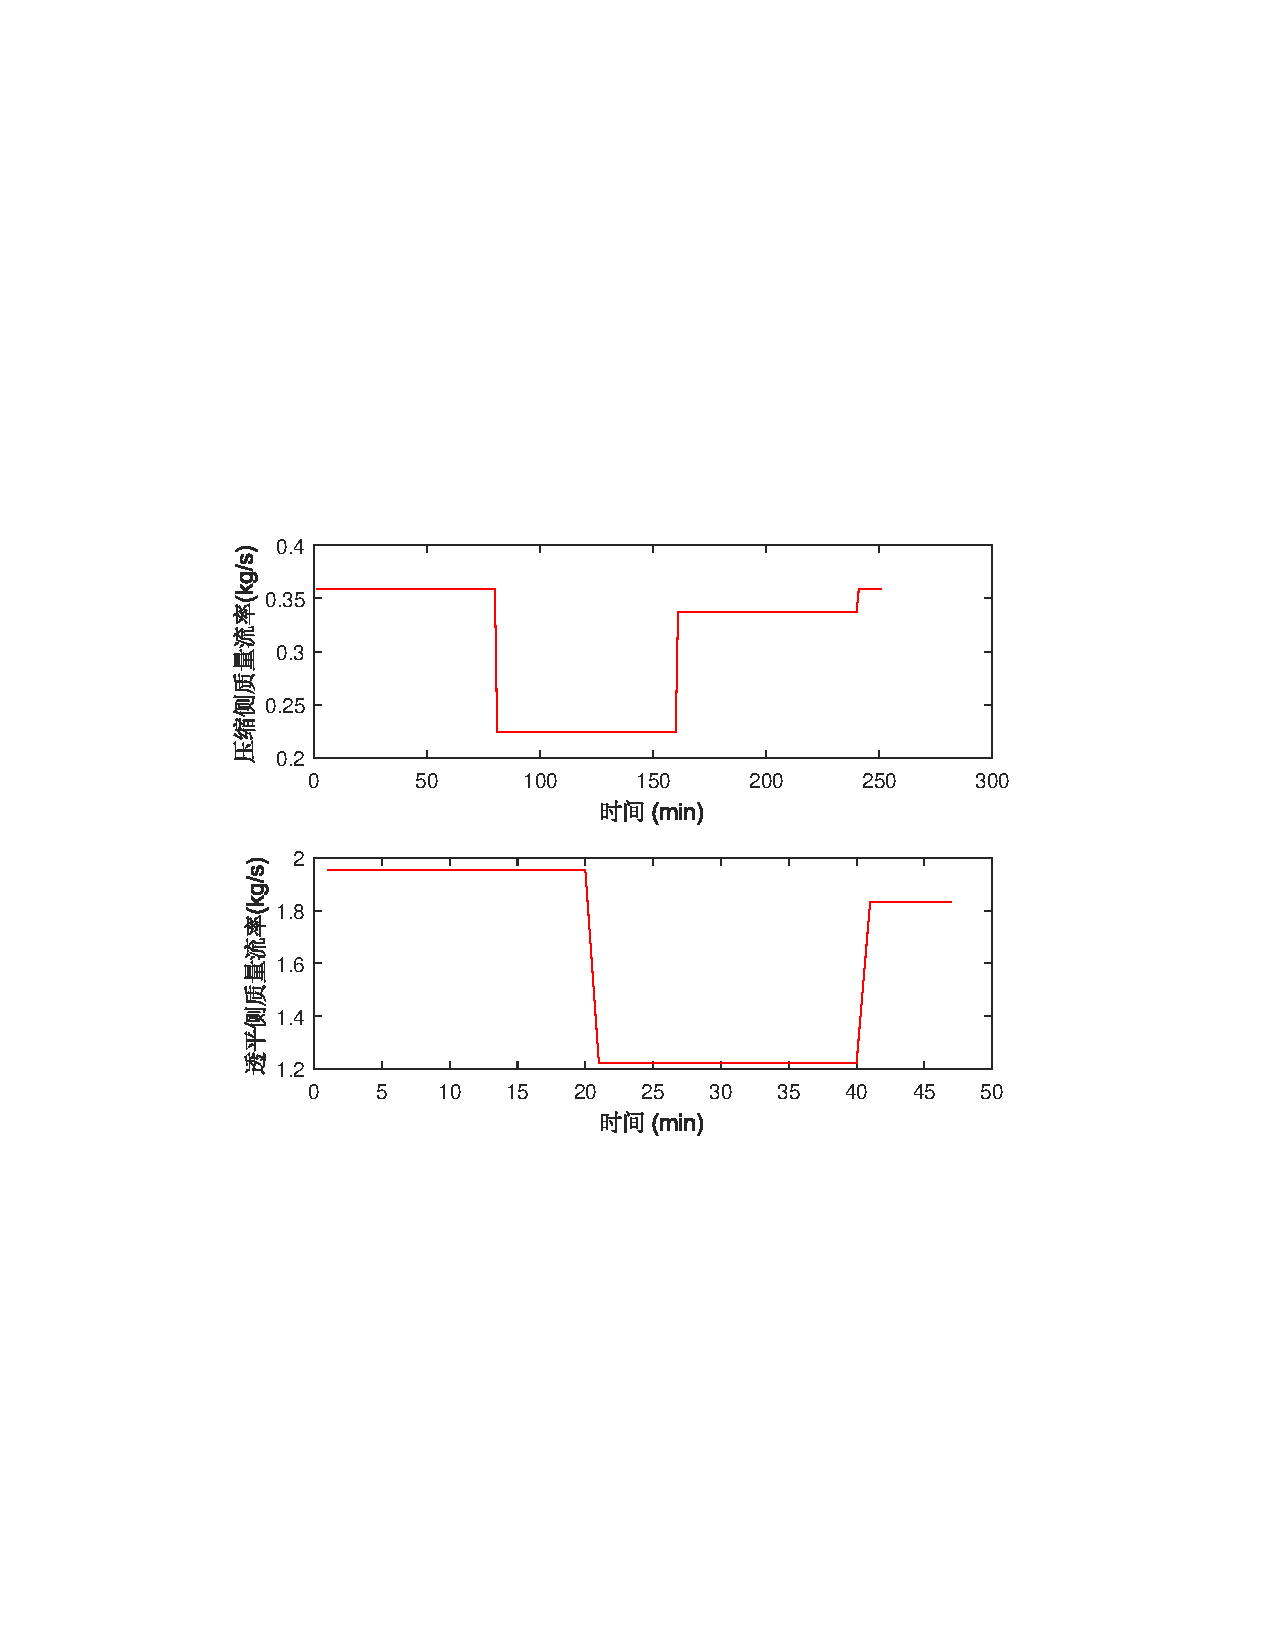
\includegraphics[scale=0.75]{Chap2-Sim-massflow-Part-load.pdf}
  \caption{模拟部分负载模式的质量流率曲线}
  \label{fig:Sim-massflow-Part-load}
\end{figure}

\subsubsection{压缩储能过程}
在压缩侧滑压运行模式下,按照图\ref{fig:Sim-massflow-Part-load}所示的质量流率进行压缩储能的过程中,压缩侧的质量流率的减小导致整个储能运行时间由设计工况下的2.9h 增长为4.18h。图\ref{fig:Sim-Char-Inlet-Pressure-Part-load}给出了部分负载运行模式下各级压缩机入口压力的变化曲线。

\begin{figure}[H] % use float package if you want it here
  \centering
  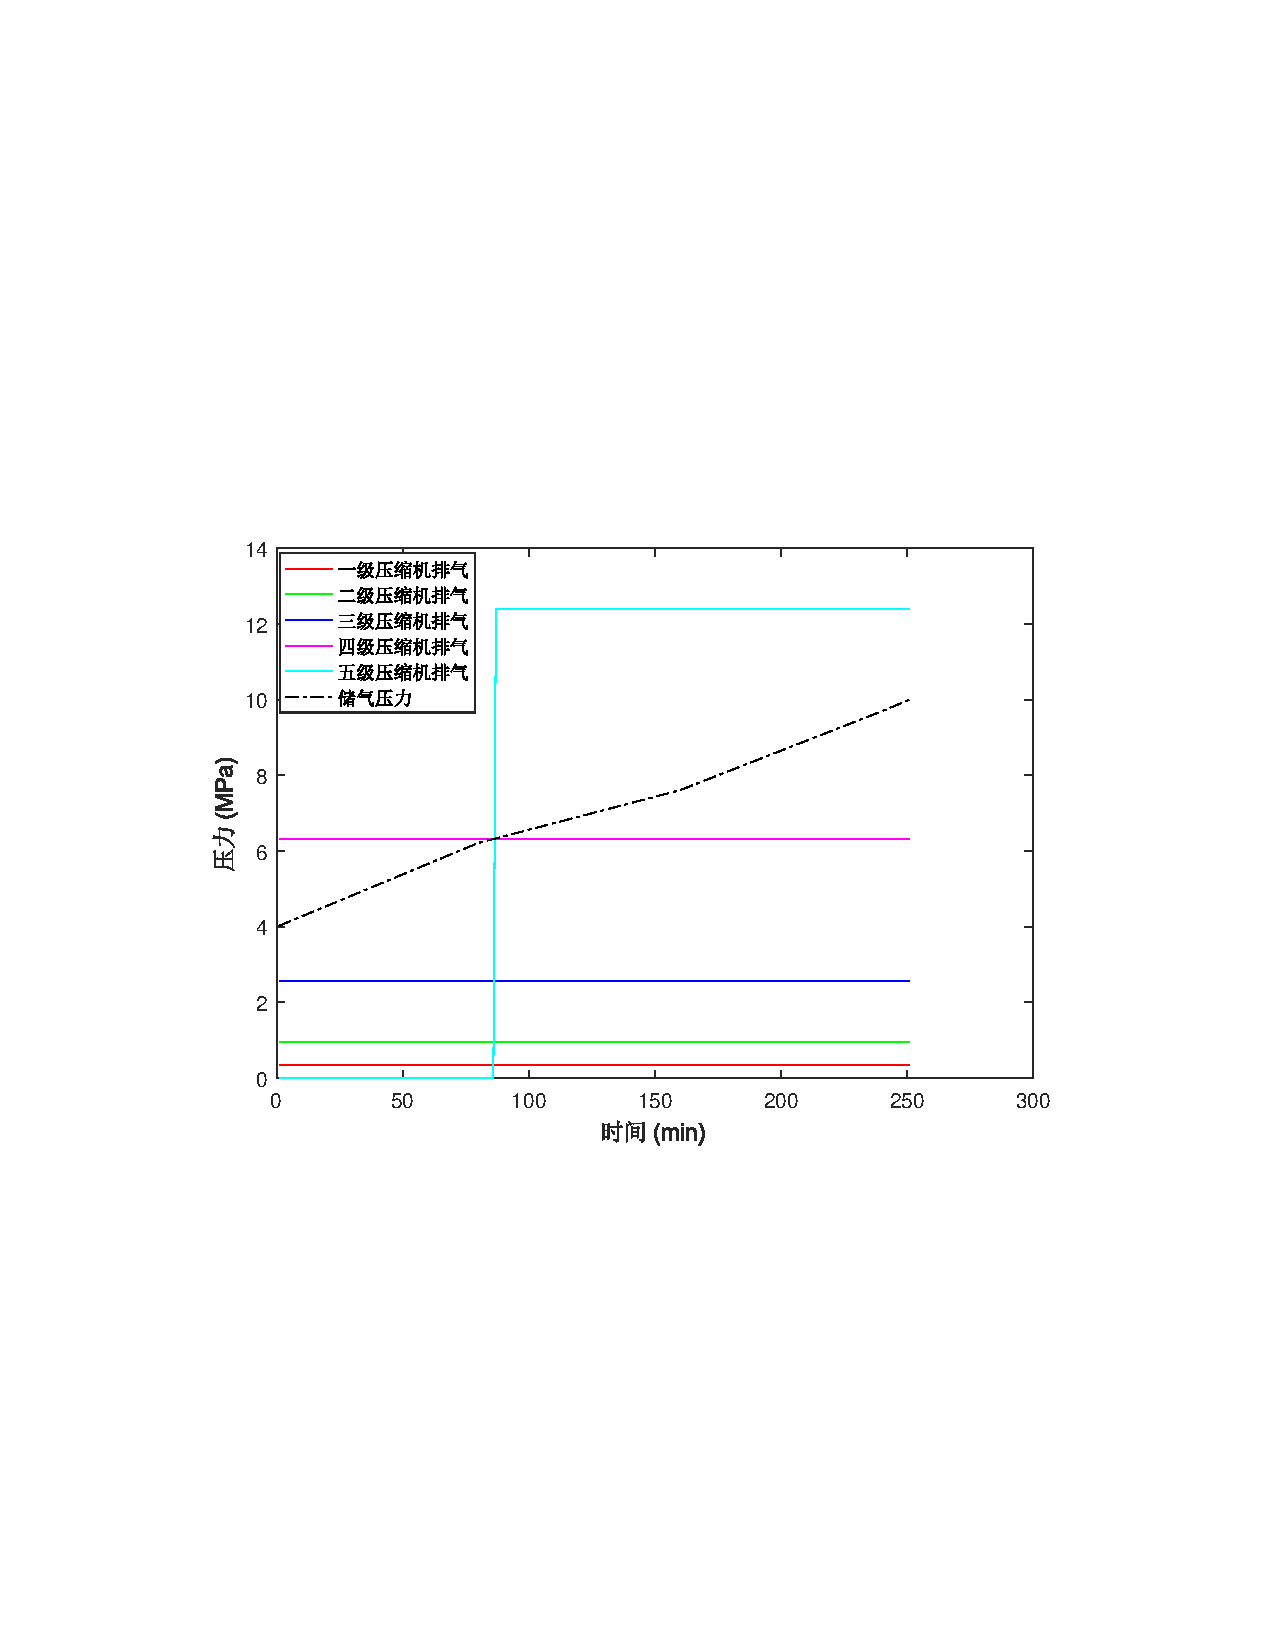
\includegraphics[scale=0.70]{Chap2-Sim-Char-Inlet-Pressure-Part-load.pdf}
  \caption{压缩储能过程压缩机入口压力变化曲线(部分负载)}
  \label{fig:Sim-Char-Inlet-Pressure-Part-load}
\end{figure}

由图\ref{fig:Sim-Char-Inlet-Pressure-Part-load}可知,储气库储气压力的变化趋势与质量流率的变化趋势一致,可近似分为三段,第一段为从0min-80min, 第二段为从81min-160min,第三段为160min-250min,相应的储气库内空气温度及空气总质量也存在同样的趋势。

\begin{figure}[H] % use float package if you want it here
  \centering
  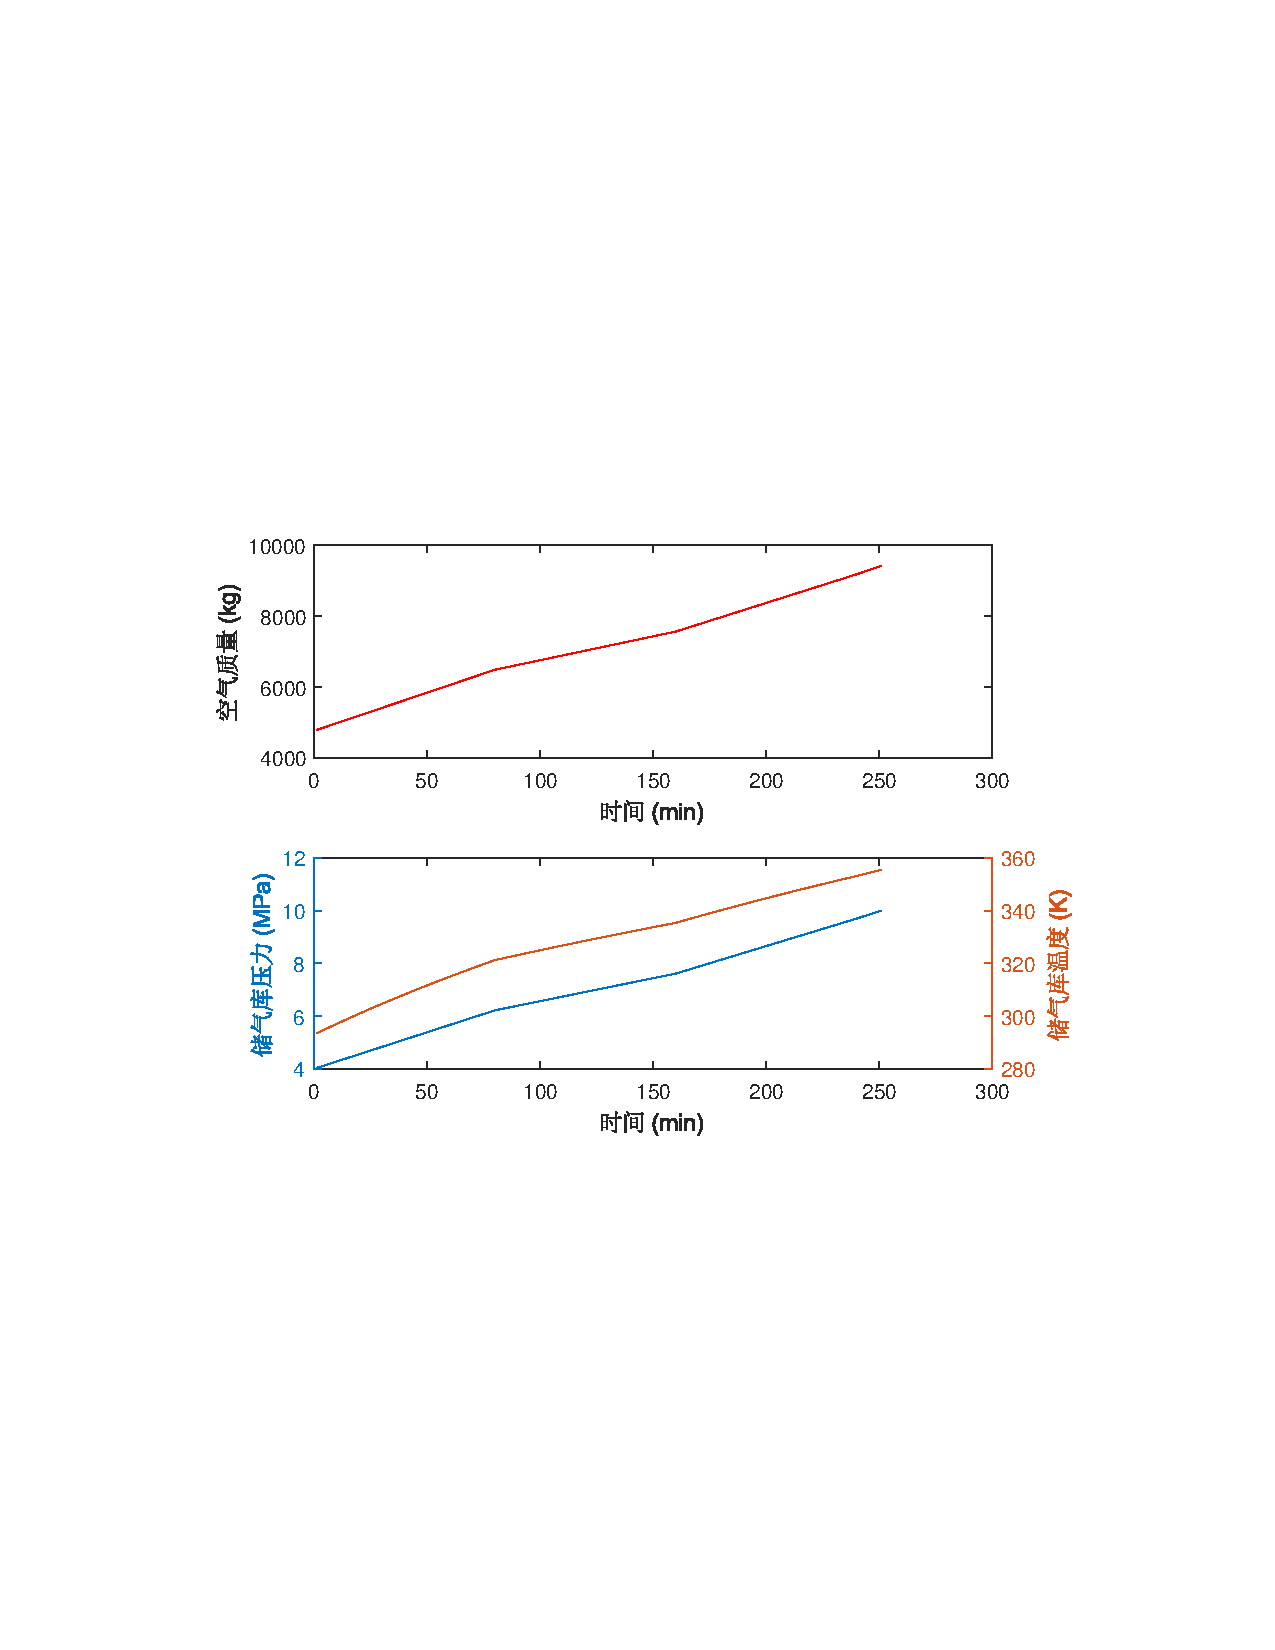
\includegraphics[scale=0.76]{Chap2-Sim-Char-ASU-Part-load.pdf}
  \caption{压缩储能过程储气库动态特性(部分负载)}
  \label{fig:Sim-Char-ASU-Part-load}
\end{figure}

图\ref{fig:Sim-Char-Heat-Quan-Part-load}给出了各级换热器换热功率的变化曲线。尽管换热器量变换趋势与质量流率趋势一致,但由于以部分负载模式运行时换热器等熵效率的降低,导致整个储热过程存储的高温HTF的降低,如图\ref{fig:Sim-Char-TES-Part-load}所示。

\begin{figure}[H] % use float package if you want it here
  \centering
  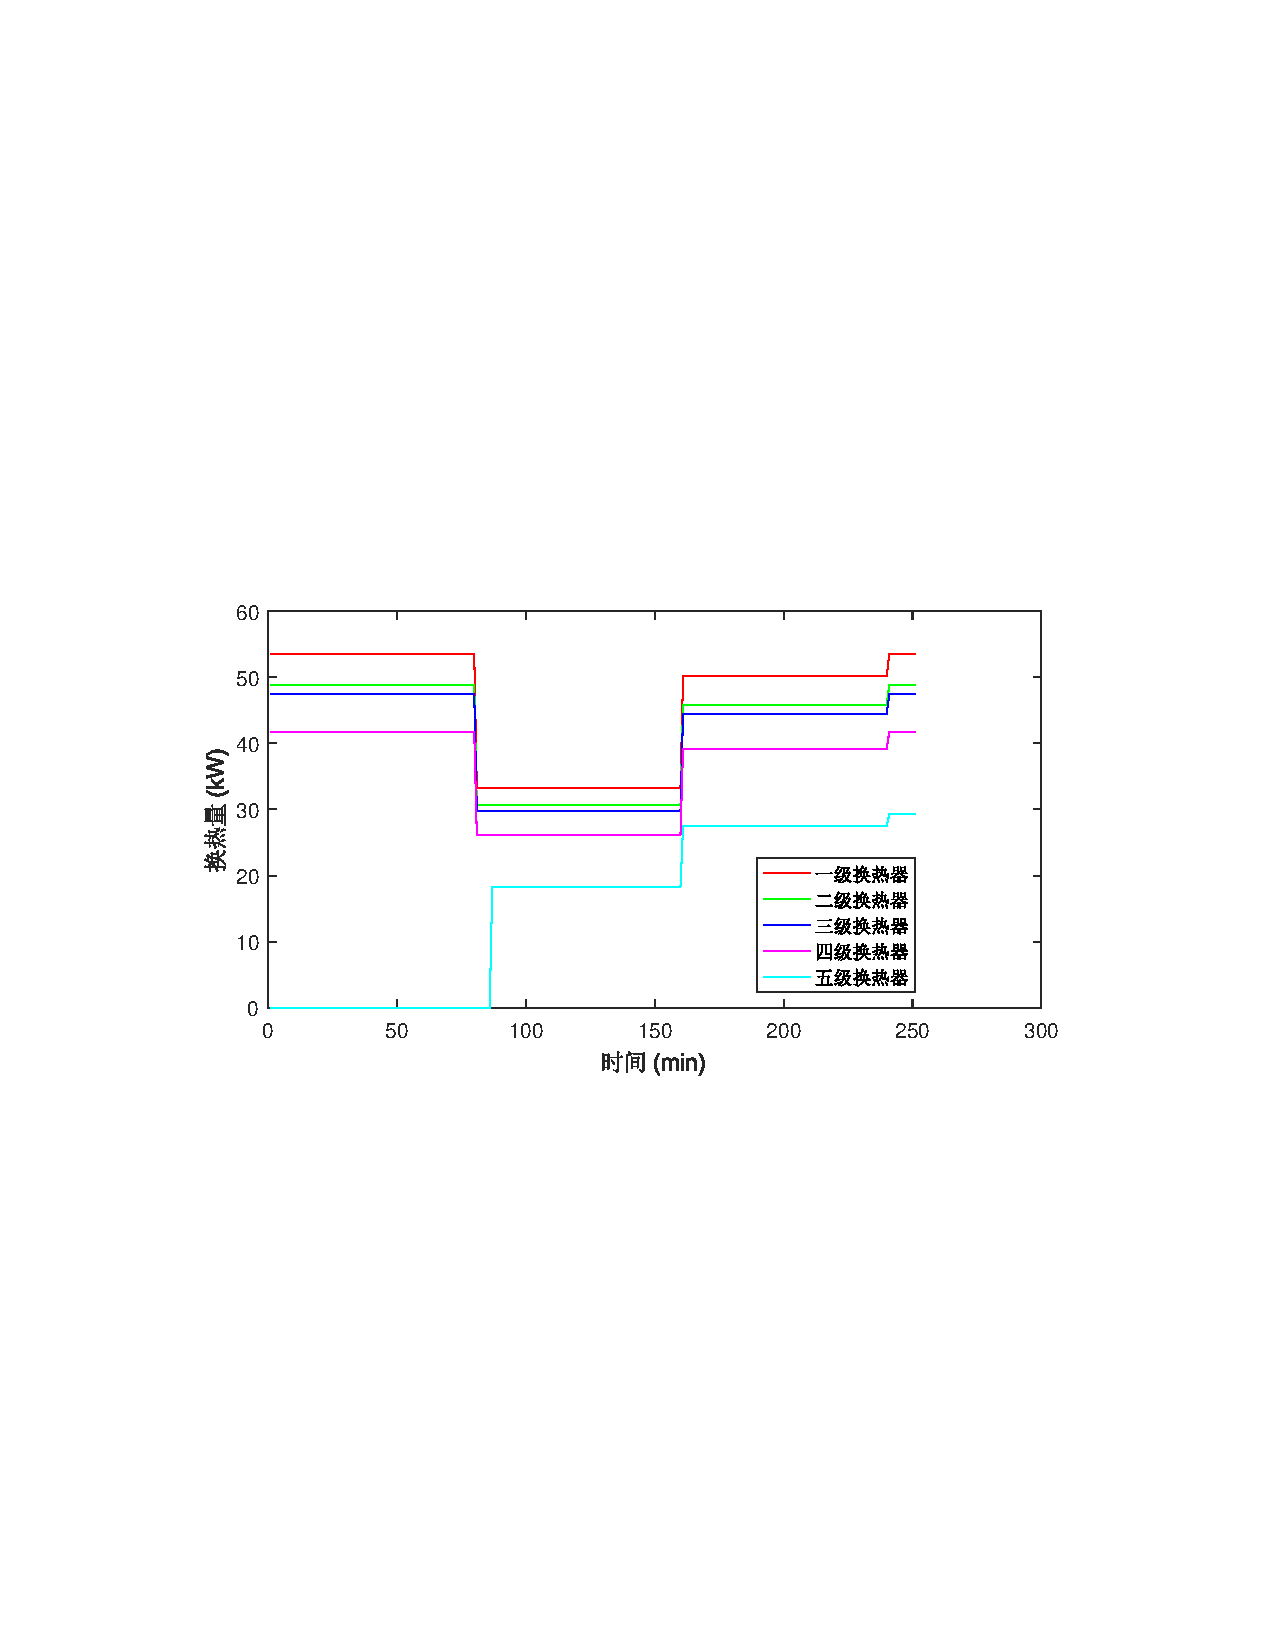
\includegraphics[scale=0.70]{Chap2-Sim-Char-Heat-Quan-Part-load.pdf}
  \caption{压缩储能过程换热器换热量变化曲线(部分负载)}
  \label{fig:Sim-Char-Heat-Quan-Part-load}
\end{figure}

压缩储能结束时储热罐中存储的储热介质质量由设计工况下的7.0973$\times 10^3$kg降为7.0407$\times 10^3$kg。与设计工况类似,由于在压缩侧滑压运行过程中第5级压缩机的启动,储热罐中HTF的温度在压缩储能过程的后期也有所降低。但是,由于在部分负载运行模式下流经换热器的HTF的质量流率相应减小,导致压缩储能结束时储热罐中HTF的温度(400.35K)稍高于设计工况(400.27K)。

\begin{figure}[H] % use float package if you want it here
  \centering
  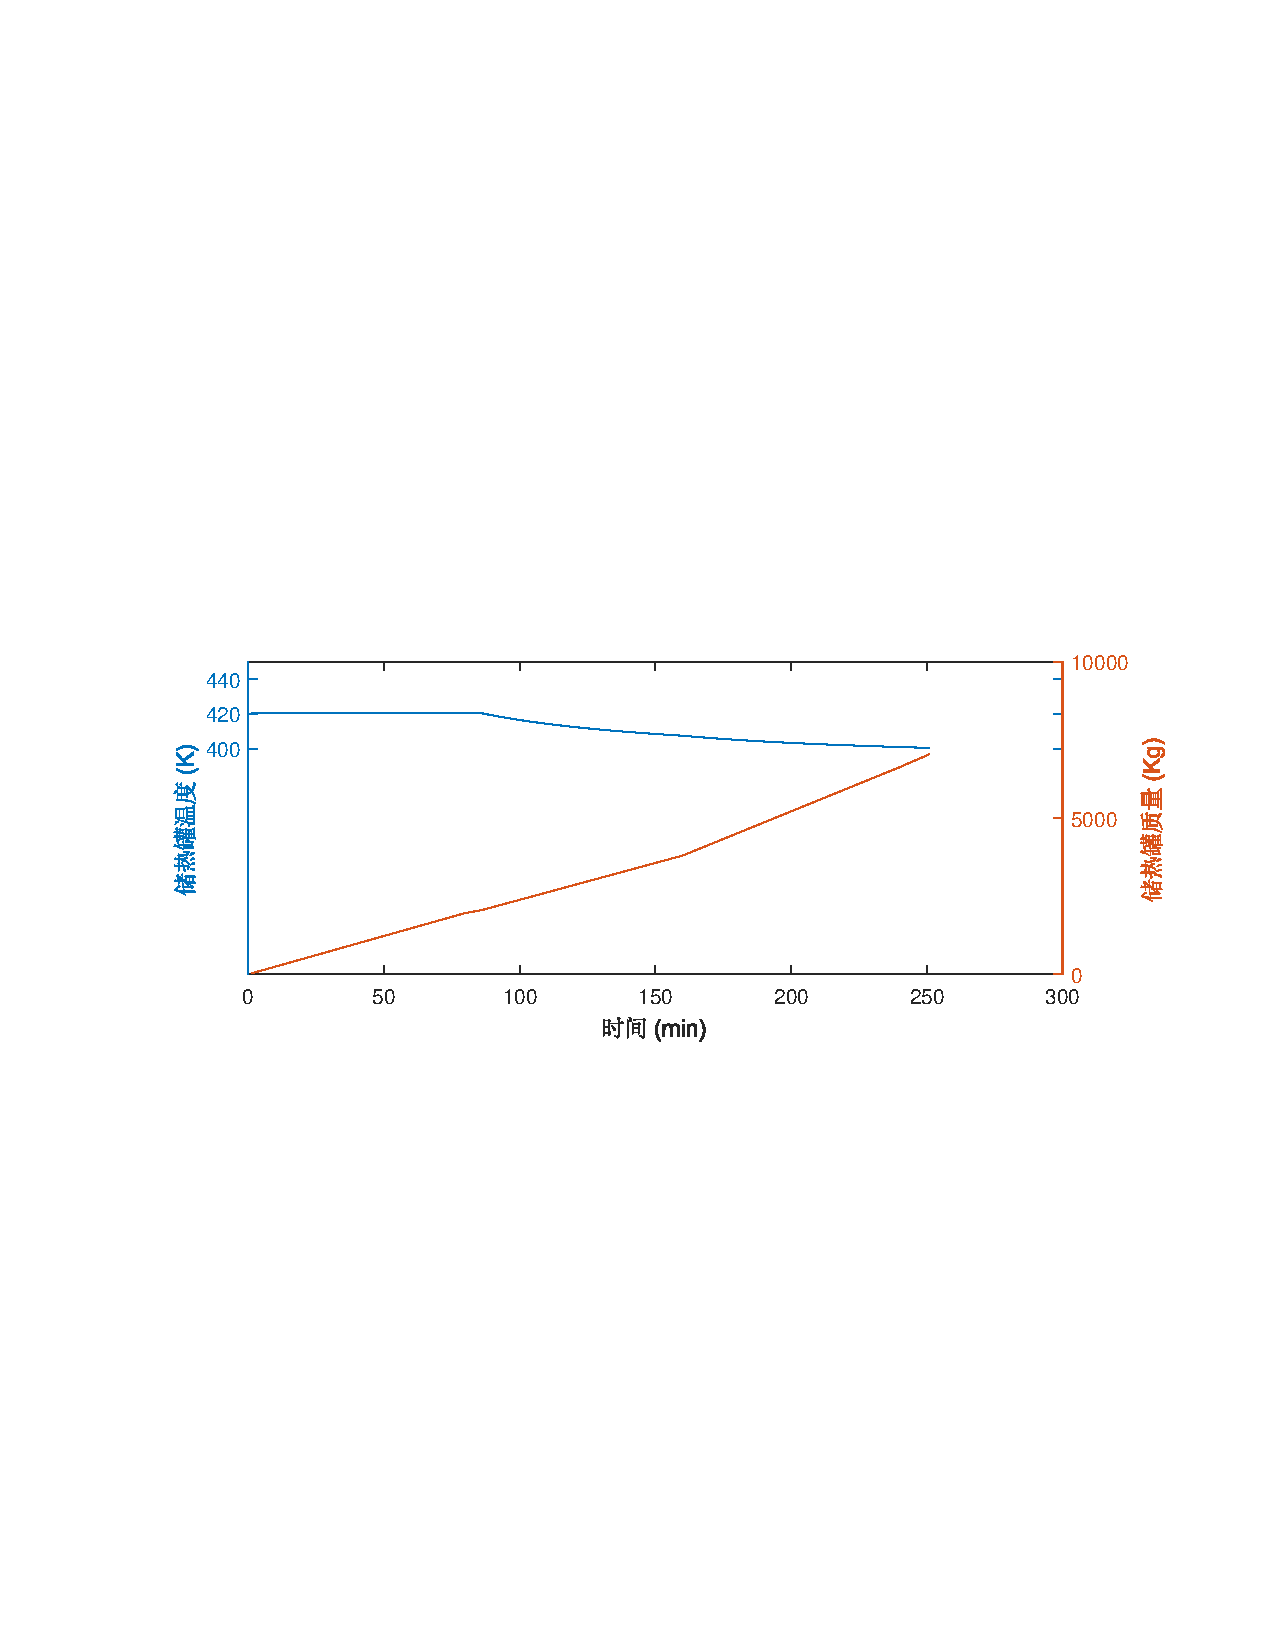
\includegraphics[scale=0.70]{Chap2-Sim-Char-TES-Part-load.pdf}
  \caption{压缩储能过程储热罐动态特性(部分负载)}
  \label{fig:Sim-Char-TES-Part-load}
\end{figure}

图\ref{fig:Sim-Char-Comp-Power-Part-load}给出了部分负载模式下压缩过程中各级压缩级的耗功。可以得出,质量流率的调节在一定程度上实现了压缩侧耗功功率的调节。在第5级压缩机未启动之前,在第81min由于压缩侧质量流率的突然减小(见图\ref{fig:Sim-massflow-Part-load}),导致压缩侧总耗功的突变,在第85min随着压缩侧背压升高,第5级压缩机启动后,压缩侧耗功回升。

\begin{figure}[H] % use float package if you want it here
  \centering
  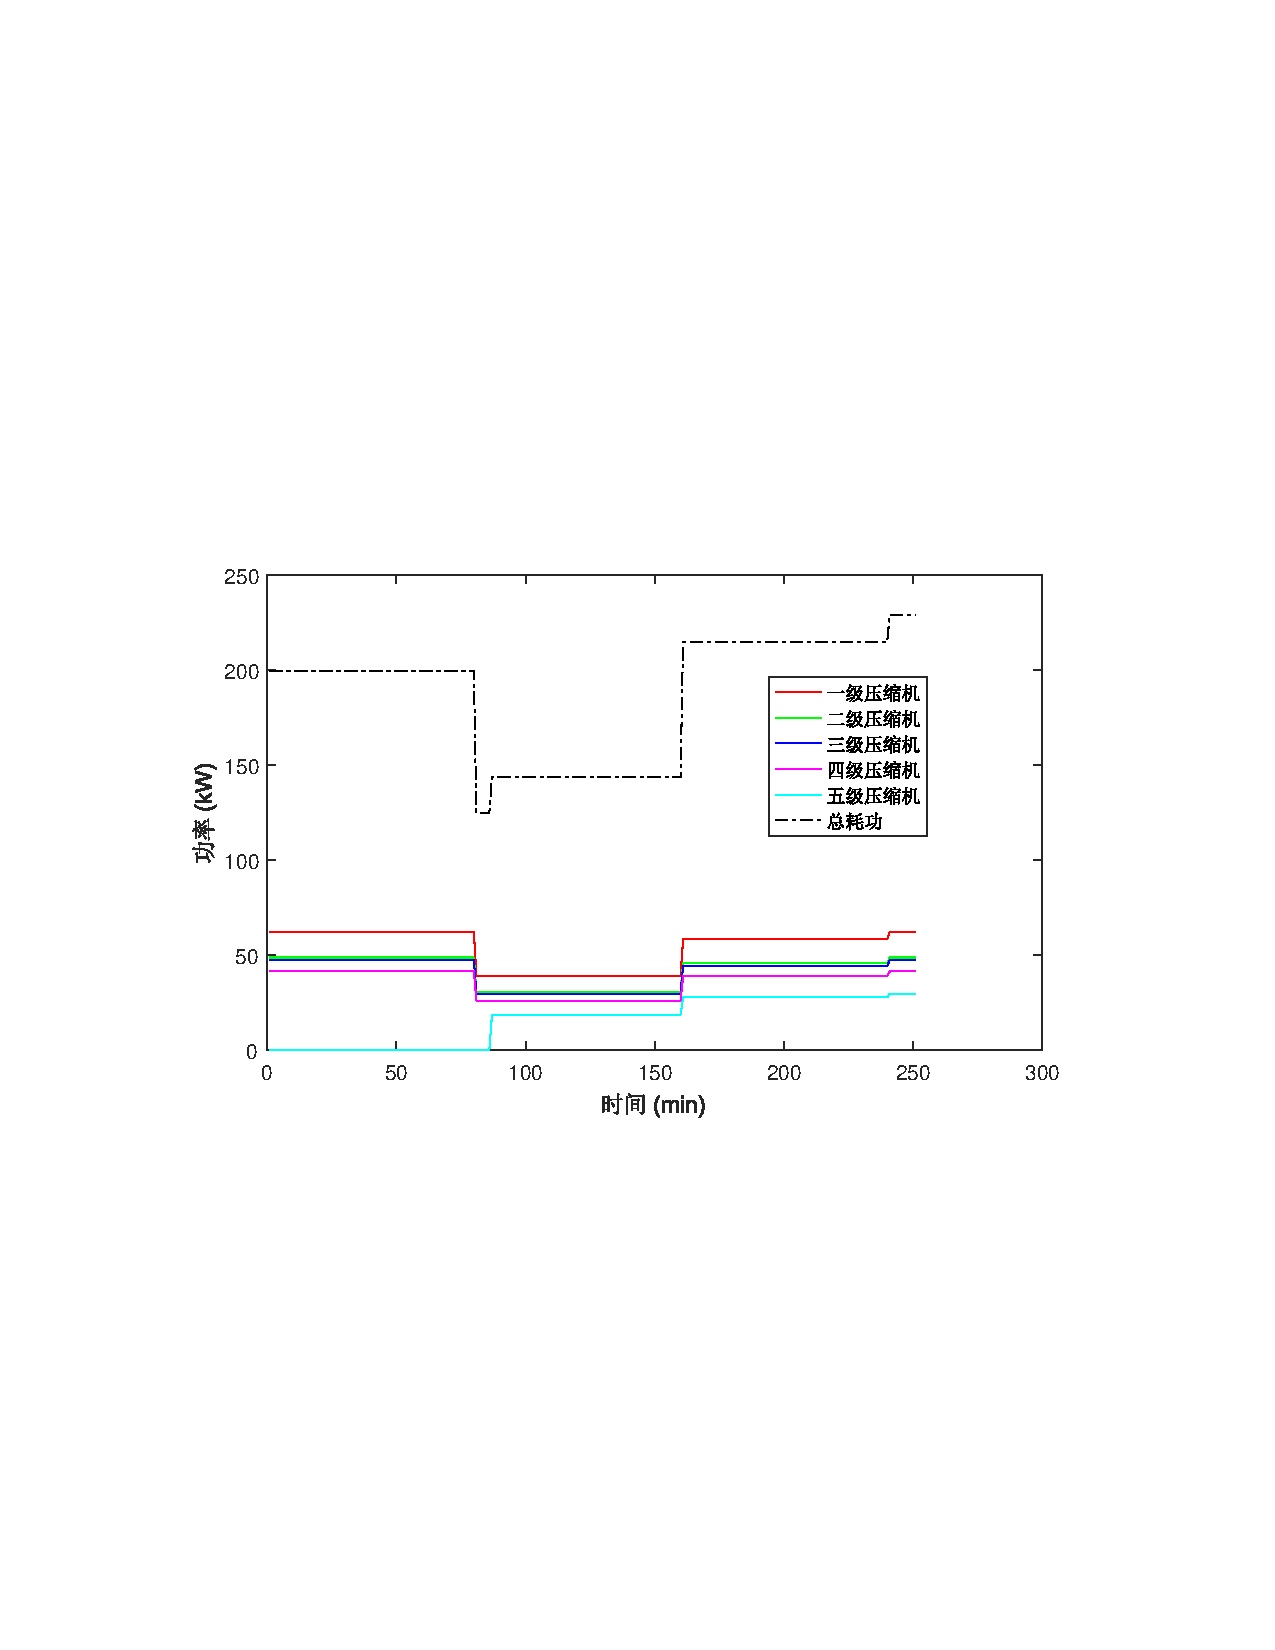
\includegraphics[scale=0.70]{Chap2-Sim-Char-Comp-Power-Part-load.pdf}
  \caption{压缩储能过程压缩机耗功变化曲线(部分负载)}
  \label{fig:Sim-Char-Comp-Power-Part-load}
\end{figure}

\subsubsection{膨胀释能过程}
在膨胀侧的定压释能过程中,按部分负载模式质量流率放气的总时间为0.78h,图\ref{fig:Sim-Disc-ASU-Pressure-Part-load}给出了整个释能过程中各级透平进气压力及储气库内空气压力的变化曲线。尽管储气库内空气压力一直在降低,但由于储气库出口侧节流阀的“稳压”作用,各级透平的进气压力均可维持核定,从而改善了由于压力偏离设计值造成的透平的部分负载运行特性。

%\subsection{适用性讨论}
\begin{figure}[H] % use float package if you want it here
  \centering
  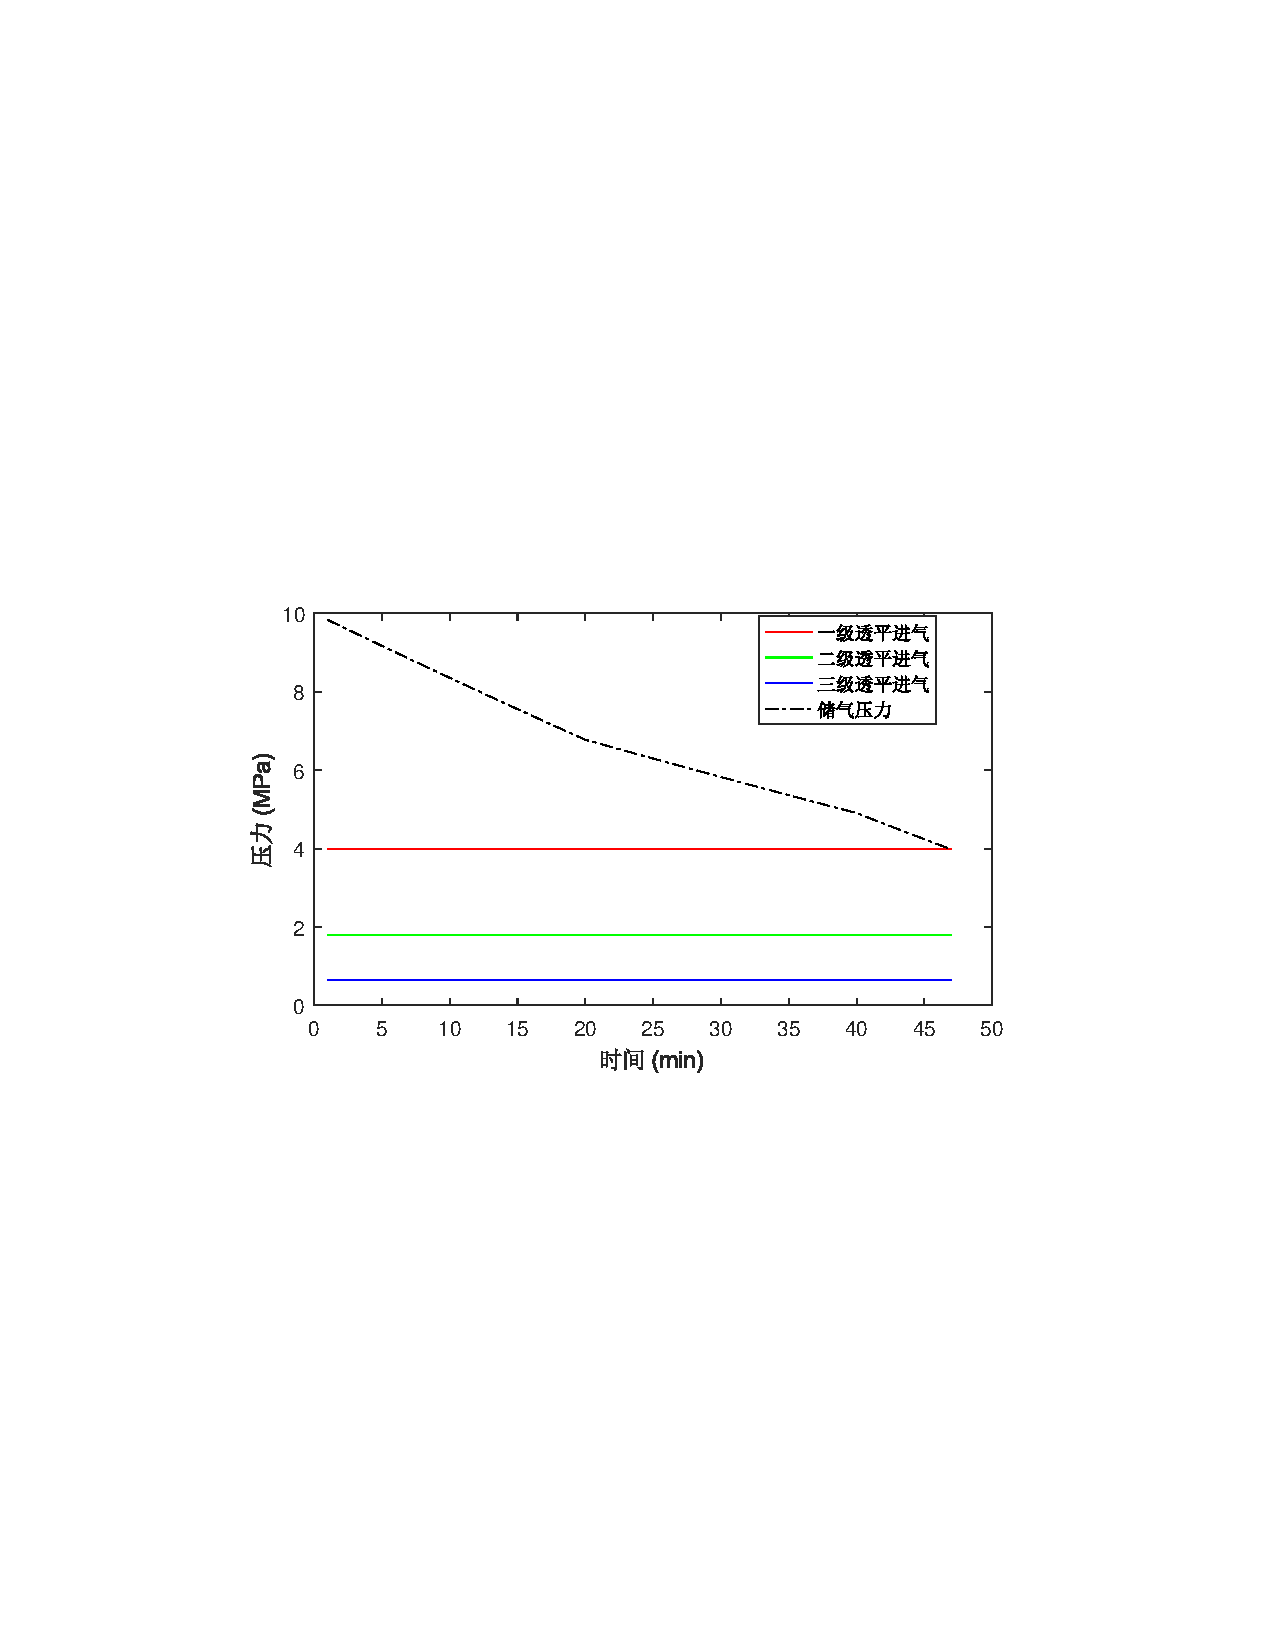
\includegraphics[scale=0.82]{Chap2-Sim-Disc-ASU-Pressure-Part-load.pdf}
  \caption{膨胀释能过程储气库动态特性(部分负载)}
  \label{fig:Sim-Disc-ASU-Pressure-Part-load}
\end{figure}

图\ref{fig:Sim-Disc-Heat-Quan-Part-load}给出了各级换热器换热功率的变化趋势。在部分负载模式下,受储气库内空气温度的变化(类似于设计工况)以及放气质量流率变化的综合影响,换热器的换热功率表现出较为复杂的特性。例如,在0-20min的释能阶段,储气库内空气温度的变化对换热器换热需求的影响占主导作用,储气库温度的降低,增加了各级换热器换热功率的需求;在第20min由于放气质量流率的降低幅度较大(见图\ref{fig:Sim-massflow-Part-load}),降低了换热器整体的换热功率需求;随着空气侧质量流率的固定,储气库温度变化对各级换热器换热的影响占主导。

\begin{figure}[H] % use float package if you want it here
  \centering
  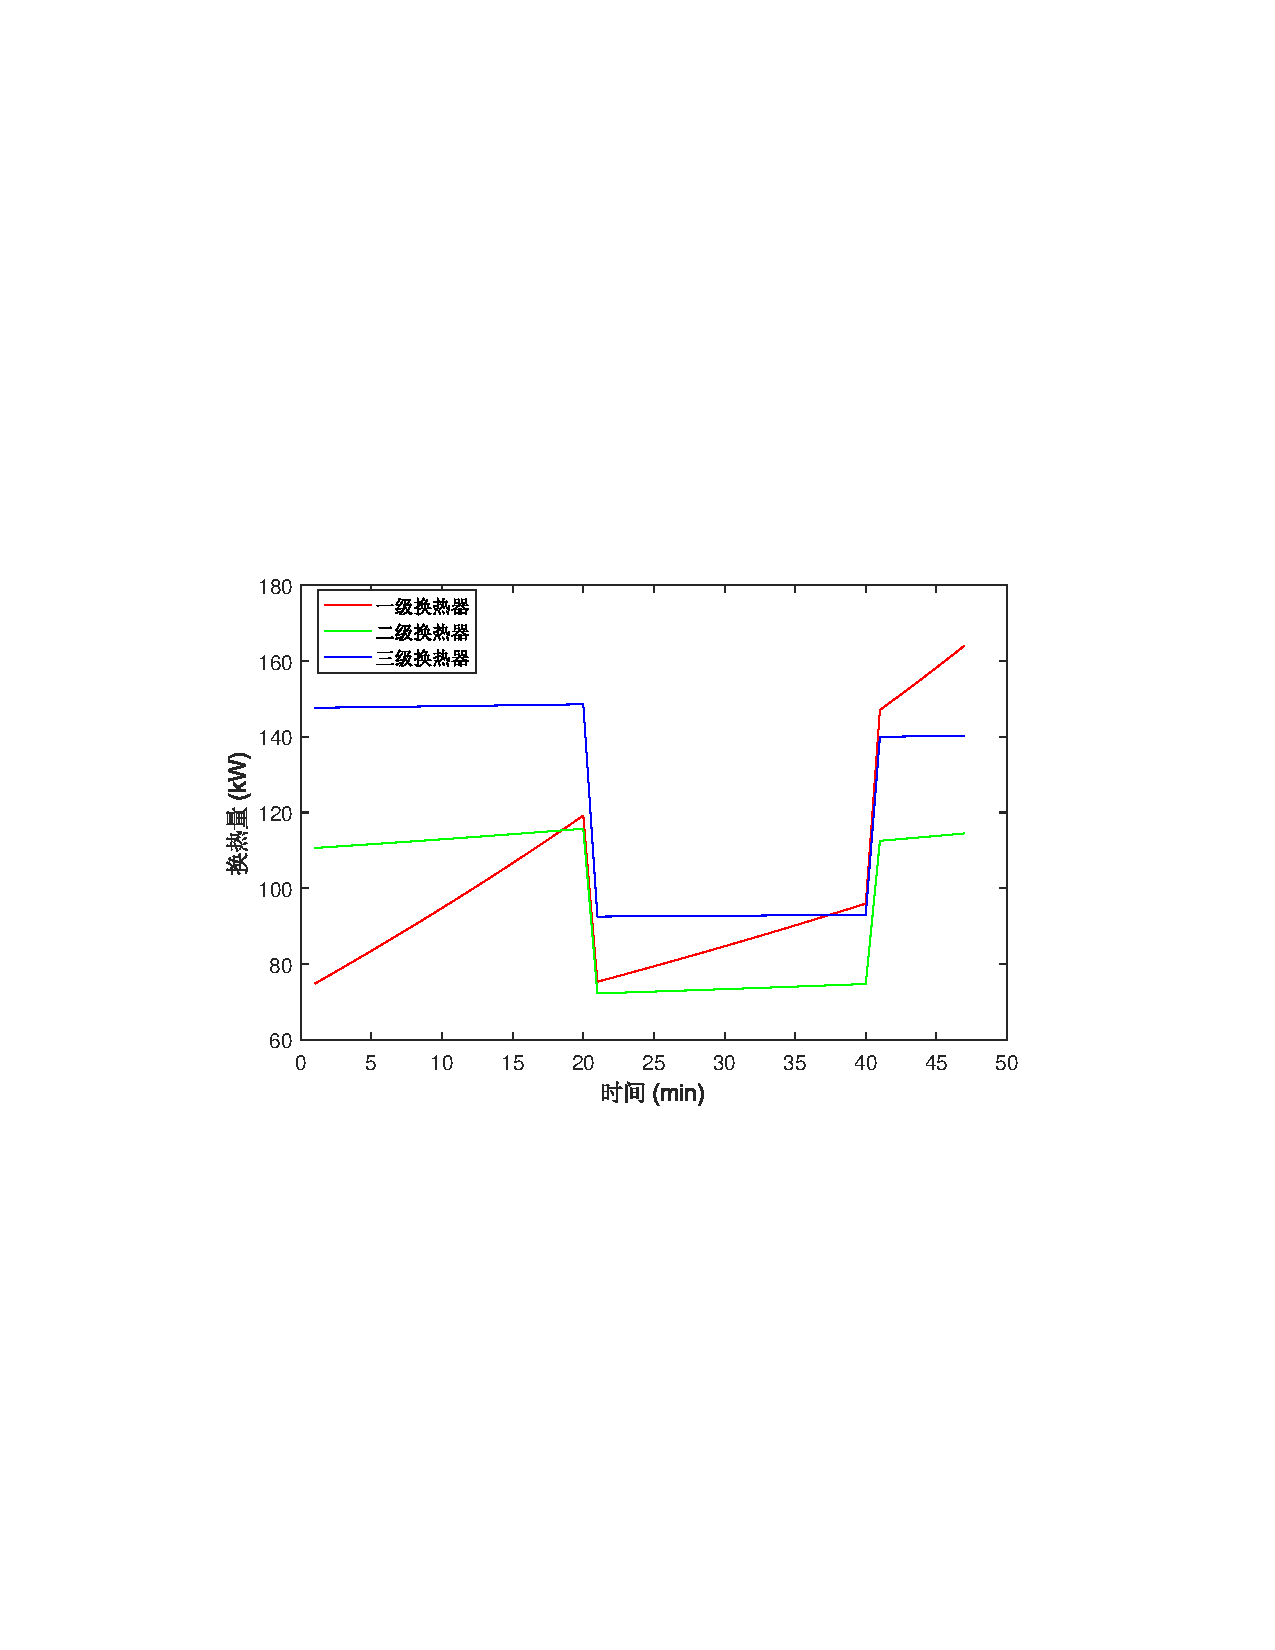
\includegraphics[scale=0.77]{Chap2-Sim-Disc-Heat-Quan-Part-load.pdf}
  \caption{膨胀释能过程换热器换热功率(部分负载)}
  \label{fig:Sim-Disc-Heat-Quan-Part-load}
\end{figure}

图\ref{fig:Sim-Disc-Turb-Power-Part-load}给出了部分负载模式下,各级透平及AA-CAES的总输出功率。由于质量流率偏离设计值,降低了释能环节透平的实际运行等熵效率,从而降低了系统输出功率。

\begin{figure}[H] % use float package if you want it here
  \centering
  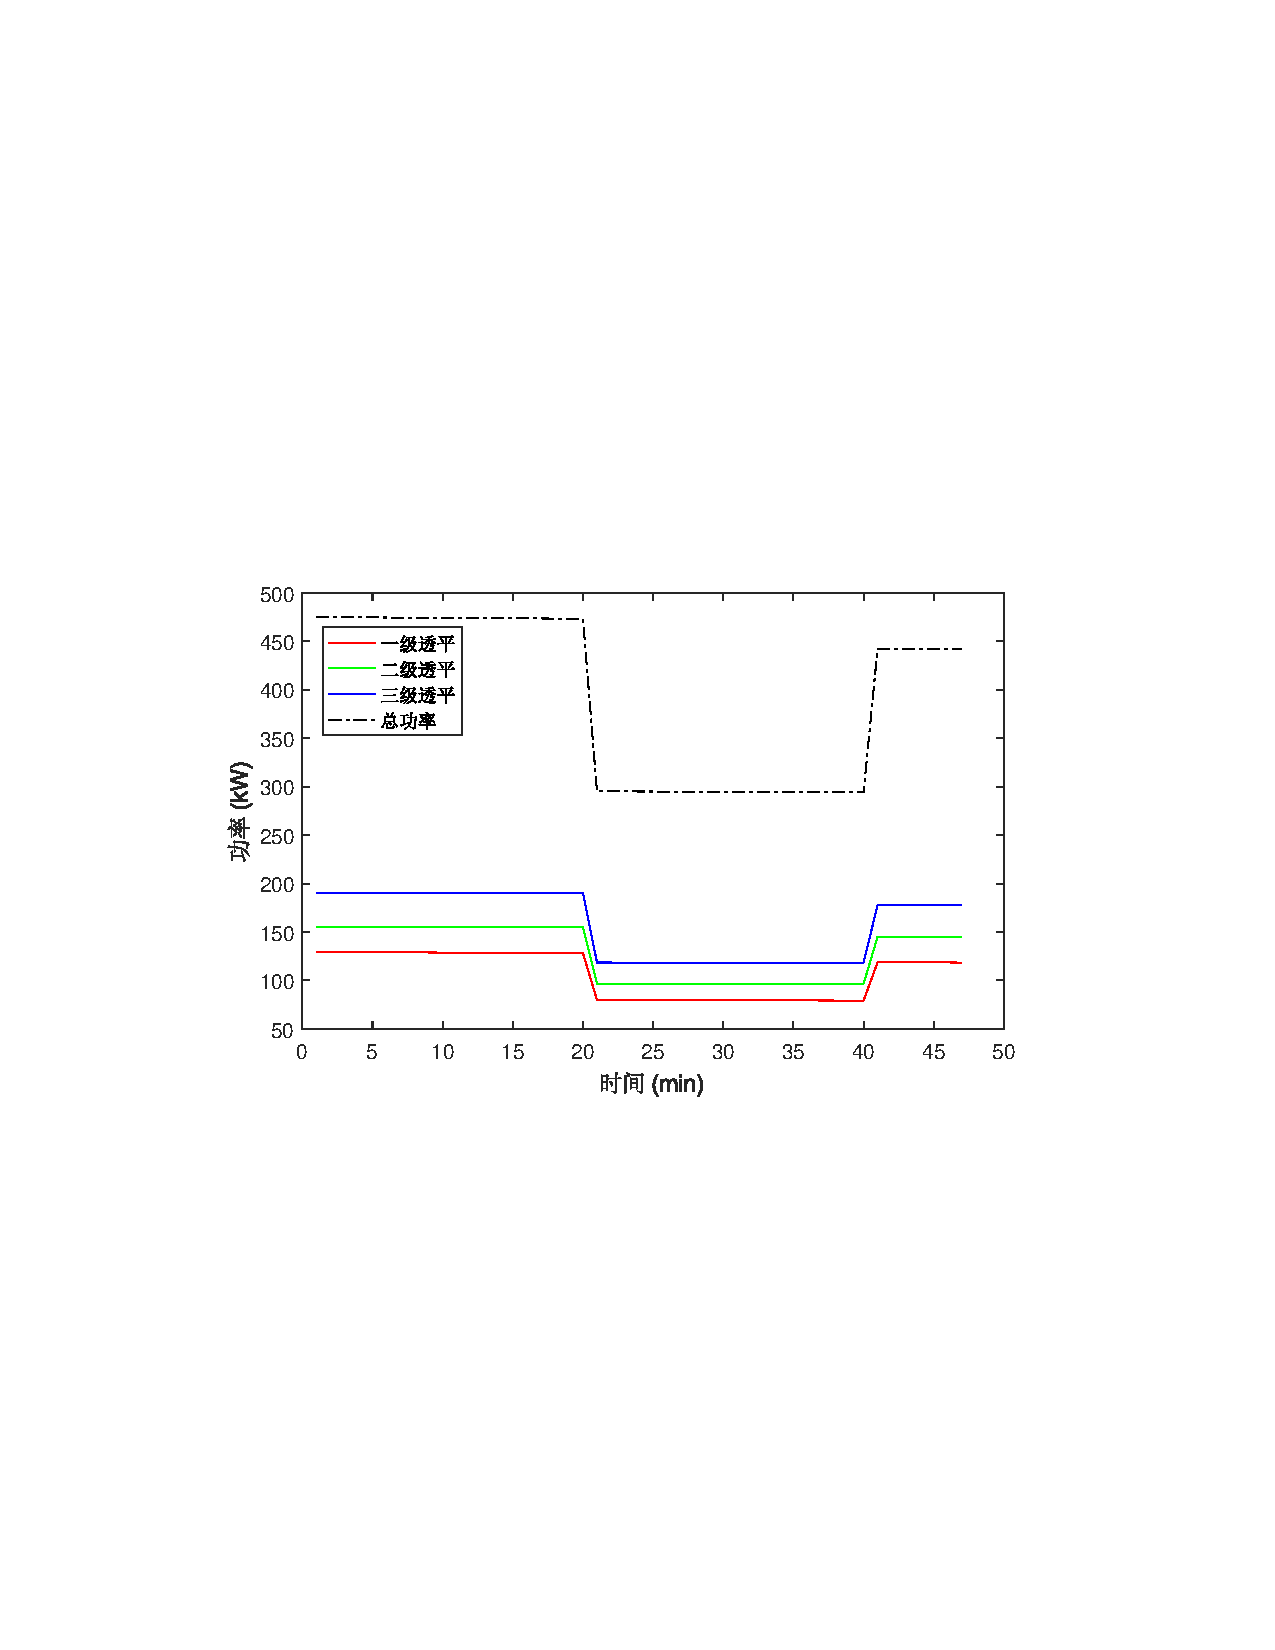
\includegraphics[scale=0.80]{Chap2-Sim-Disc-Turb-Power-Part-load.pdf}
  \caption{膨胀释能过程输出功率变化曲线(部分负载)}
  \label{fig:Sim-Disc-Turb-Power-Part-load}
\end{figure}

综上,以本节给定的部分负载质量流率进行压缩储能与膨胀释能的一个循环周期中,AA-CAES消耗的总电量为0.8259MWh,输出的总电量为0.3079MWh,其电-电效率$\eta_{elec}$ 为37.28\%,与设计工况相比相对下降6.87\%。储能结束时高温储热罐中的HTF质量为7.0407$\times10^3$kg,释能结束时储热罐中剩余的HTF质量为3.3266$\times10^3$kg,温度为400.35K,可用于供热的热量为0.3563MW,供热效率为$\eta_{heat}$为43.14\%,系统热电热联供的总能利用系数$\eta_{total}$为80.42\%。供热的热量㶲为0.0955MWh,供热㶲效率为11.56\%,总㶲效率为48.58\%。对比设计工况与宽工况算例可知,部分负载运行模式降低了系统的电-电效率、总能利用系数以及总㶲效率。需要说明的是,在本节的仿真中我们采用了小容量的AA-CAES系统,其储气与储热系统均能实现绝热,若考虑储气库及储热系统的传热损失,则上述分析中的效率指标均会有所下降。

\section{小结}
实现面向宽工况应用的AA-CAES准确的组件级部分负载热力学特性建模与分析是研究AA-CAES运行模型及市场运营策略等的前提。本章结合新能源电力系统中AA-CAES的典型应用场景对其宽工况运行的要求,以及由此导致的内部组件级别的部分负载特性,建立了AA-CAES通用宽工况热力学稳态仿真模型。同时,基于构建的热力学仿真模型分析了一典型AA-CAES试验系统在多种运行模式及多种供能模式下的运行特性,为源-网-荷侧相应AA-CAES实现形式的建模与分析提供了基础。

\chapter{网侧先进绝热压缩空气储能电站建模及运行方法}
\label{cha:aa-caes}

\section{概述}
\label{sec:aa-caes-intro}
~AA-CAES~在新能源电力系统中最基本的应用形式即为储能电站,可用于电网削峰填谷、调峰、备用等场景\cite{CAES-DAM-Rui-18}。AA-CAES能用于该类场景的主要原因在于其能为电网提供较长时间的能量及容量备用等灵活性支撑(见图\ref{fig:CAES-AS-Overview}),而实现~AA-CAES~储能电站能量与备用特性的准确建模是分析其在电力系统中运行特性的前提。

构建能量与备用模型最直观的思路是采用等效电池模型,然而本文第\ref{cha:simulation}章指出备用等运行模式需要AA-CAES储能电站运行于宽工况条件,导致内部组件处于部分负载运行模式,而等效电池模型难以刻画组件级的部分负载特性。另一方面,完全采用第\ref{cha:simulation}章的部分负载热力学仿真模型构建的能量与备用模型又过于复杂,难以被实际AA-CAES储能电站及所在电力系统的运行调度所采用。为此,我们需要寻求一种既不丢失AA-CAES的宽工况热力学特性且物理意义简单明确的运行建模方法,以实现等效电池模型与热力学仿真模型之间的平衡。

借鉴数据结构的思想,若将AA-CAES视为对象,其属性可视为第2章研究的每个组件,而其方法为各组件的部分负载热力学特性。只要通过合适的接口设计,使得AA-CAES这一对象对外提供能表征其内部热力学特性,且对外部应用而言物理意义明确、形式简单的典型接口函数,即可实现复杂的热力学仿真模型与电力等效电池模型间的平衡。本章将该类接口函数称为热力学特性曲线簇,其可实现对内部组件级部分负载特性的封装,同时对外提供了获取AA-CAES系统宽工况运行特性的接口,可供储能电站的调度运行及市场运营等问题使用。

本章结构安排如图~\ref{fig:AA-CAES-Flow-Chart}所示,第~\ref{sec:chap3-aa-caes-sim}节基于第~\ref{cha:simulation} 章组件级部分负载热力学仿真模型,提出表征AA-CAES宽工况运行特性的热力学特性曲线簇;第\ref{sec:dual-SOC}节基于宽工况特性曲线簇,提出计及储气水平与储热水平及二者耦合关系的双~SOC~建模框架与方法;第
\ref{sec:chap3-wind-ESS-operation}节基于双~SOC~模型分析宽工况特性对风-储协同系统运行的影响;第\ref{sec:chap3-bid-aa-caes}节给出AA-CAES储能电站的市场运营策略,以提升储能电站运行经济性。

\begin{figure}[H] % use float package if you want it here
  \centering
  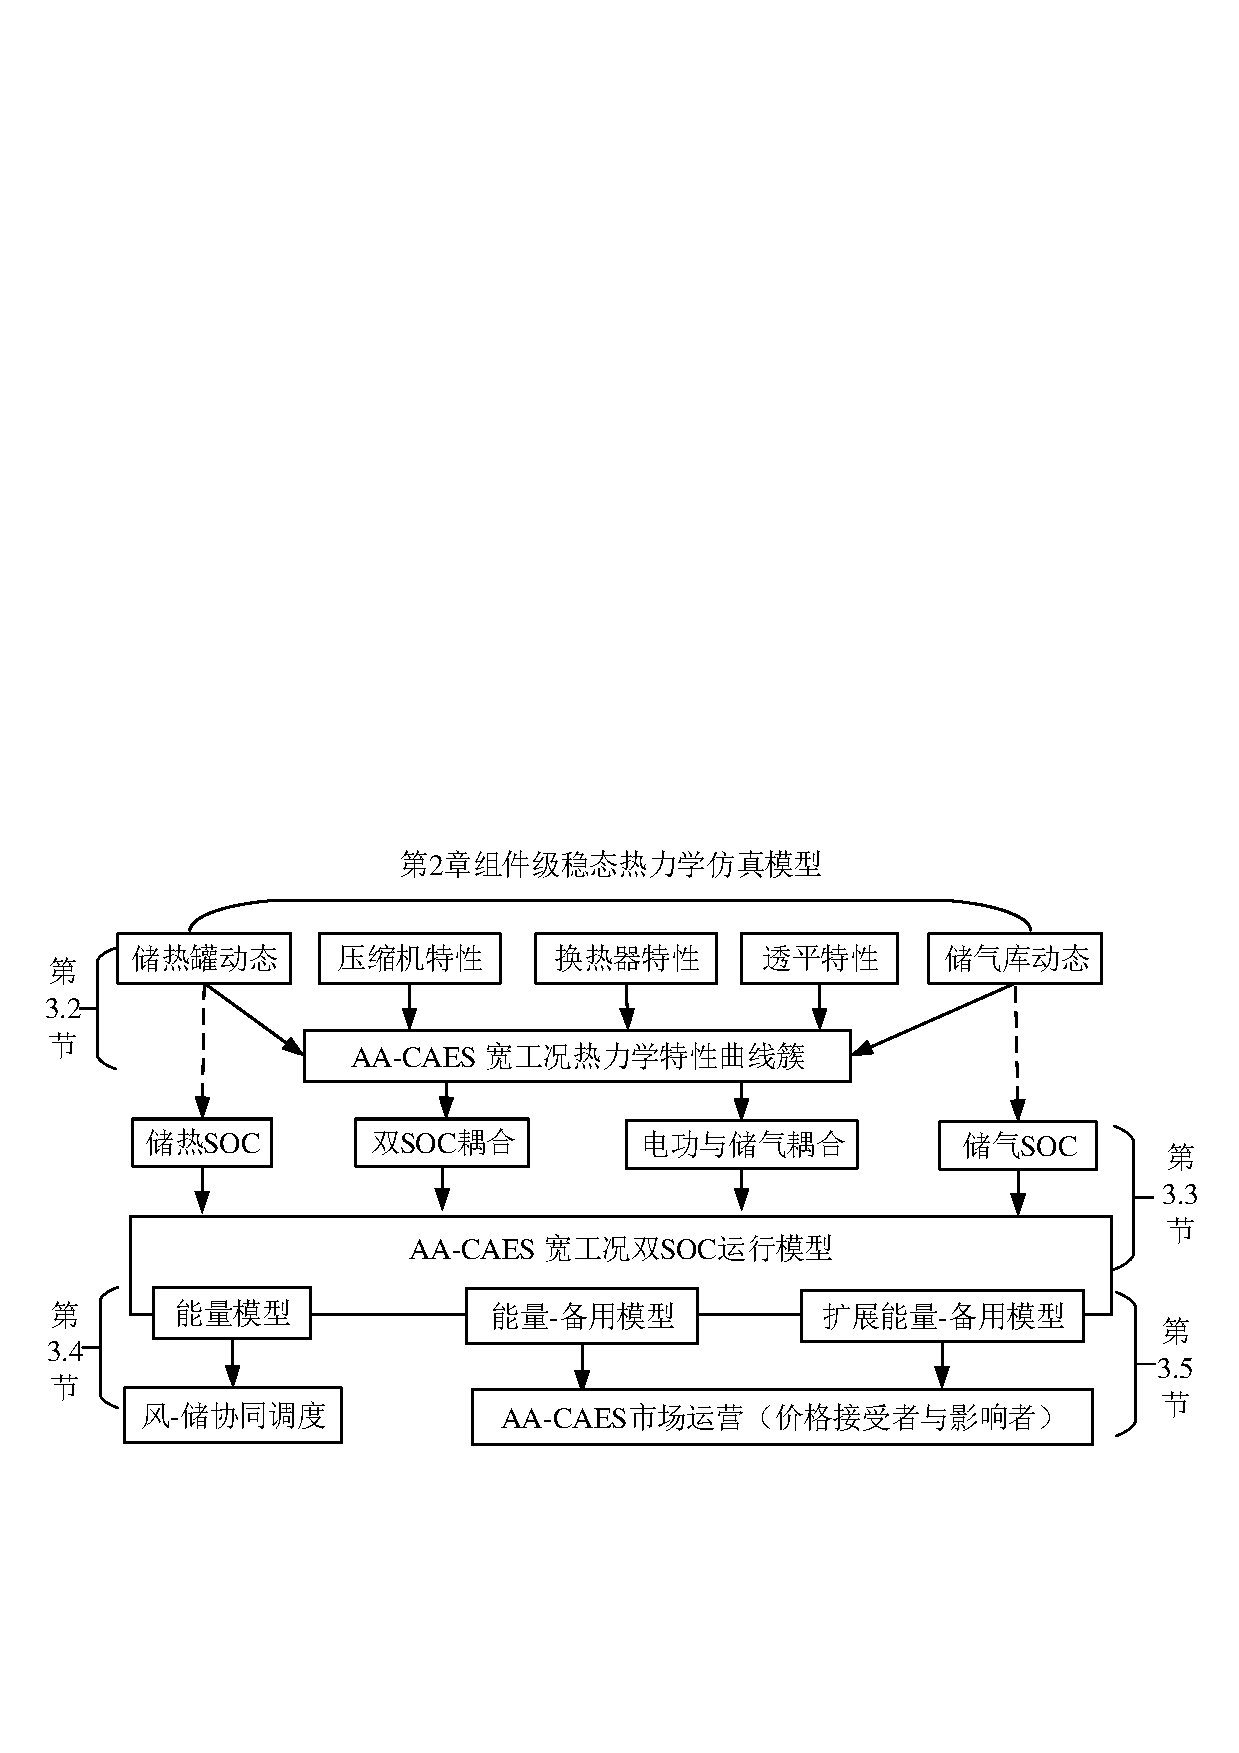
\includegraphics[scale=0.72]{figures/Chap3-1-AA-CAES-Flow-Chart-V4.pdf}
  \caption{第~\ref{cha:aa-caes}~章结构安排}
  \label{fig:AA-CAES-Flow-Chart}
\end{figure}

\section{宽工况热力学特性曲线簇}
\label{sec:chap3-aa-caes-sim}
本节基于第\ref{cha:simulation}章宽工况热力学仿真模型抽象出能刻画AA-CAES内部组件的部分负载特性对系统宽工况运行特性整体影响的热力学特性曲线簇。首先,分析AA-CAES 内部组件级(压缩机、膨胀机、换热器)部分负载特性的集中化表示思路;其次,从换热器视角给出AA-CAES内部压力势能与压缩热能双能流耦合关系的集中模型;最后,从压缩机与膨胀机视角给出储气量与压缩/膨胀功率间的耦合关系,从而界定四组通用的AA-CAES宽工况热力学特性曲线簇。

\subsection{组件级部分负载特性的集中表示}
压缩机、空气透平及换热器等组件的部分负载运行特性,一般由AA-CAES储能电站的系统集成者在压缩机、透平及换热系统选型阶段予以克服或优化设计。对电力系统运行调度人员而言,需要关注内部组件的部分负载特性对AA-CAES储能电站与电网的功率接口(即压缩机的压缩功率与透平的膨胀功率)的整体影响。

鉴于已有商业化运行数据(或经验),我们先分析D-CAES电站的运行特性,进而推广到AA-CAES储能电站。因D-CAES电站仅存储高压空气,释能环节所需热量由相对灵活的外界燃料补燃提供,其储(电)能水平可通过储气库储气水平(唯一)决定~\cite{CAES-Review-18-Rui-operation}。以采用滑压-定压模式运行的D-CAES电站为例,其在释能过程中不同膨胀功率下单位输出电功率消耗的高压空气质量流率受其空气透平的部分负载运行特性影响,在储能过程中不同压缩功率下单位输入电功率能存储的高压空气质量流率受压缩机的部分负载特性与储气库储气的水平共同影响。基于文献\inlinecite{CAES-Discharge-16}和\inlinecite{CAES-Reserve-Bid-Therm-16}中的测试数据,图\ref{fig:Compression-SOC-Part-Load}给出了不同储能水平下D-CAES电站单位压缩功率所能存储的压缩空气质量(空气压力势能)的变化曲线,在D-CAES电站的实际运行中可根据储气库空气的压力、温度等热力学参数调节补燃环节的供热量即可实现高效的膨胀释能。

\begin{figure}[H] % use float package if you want it here
  \centering
  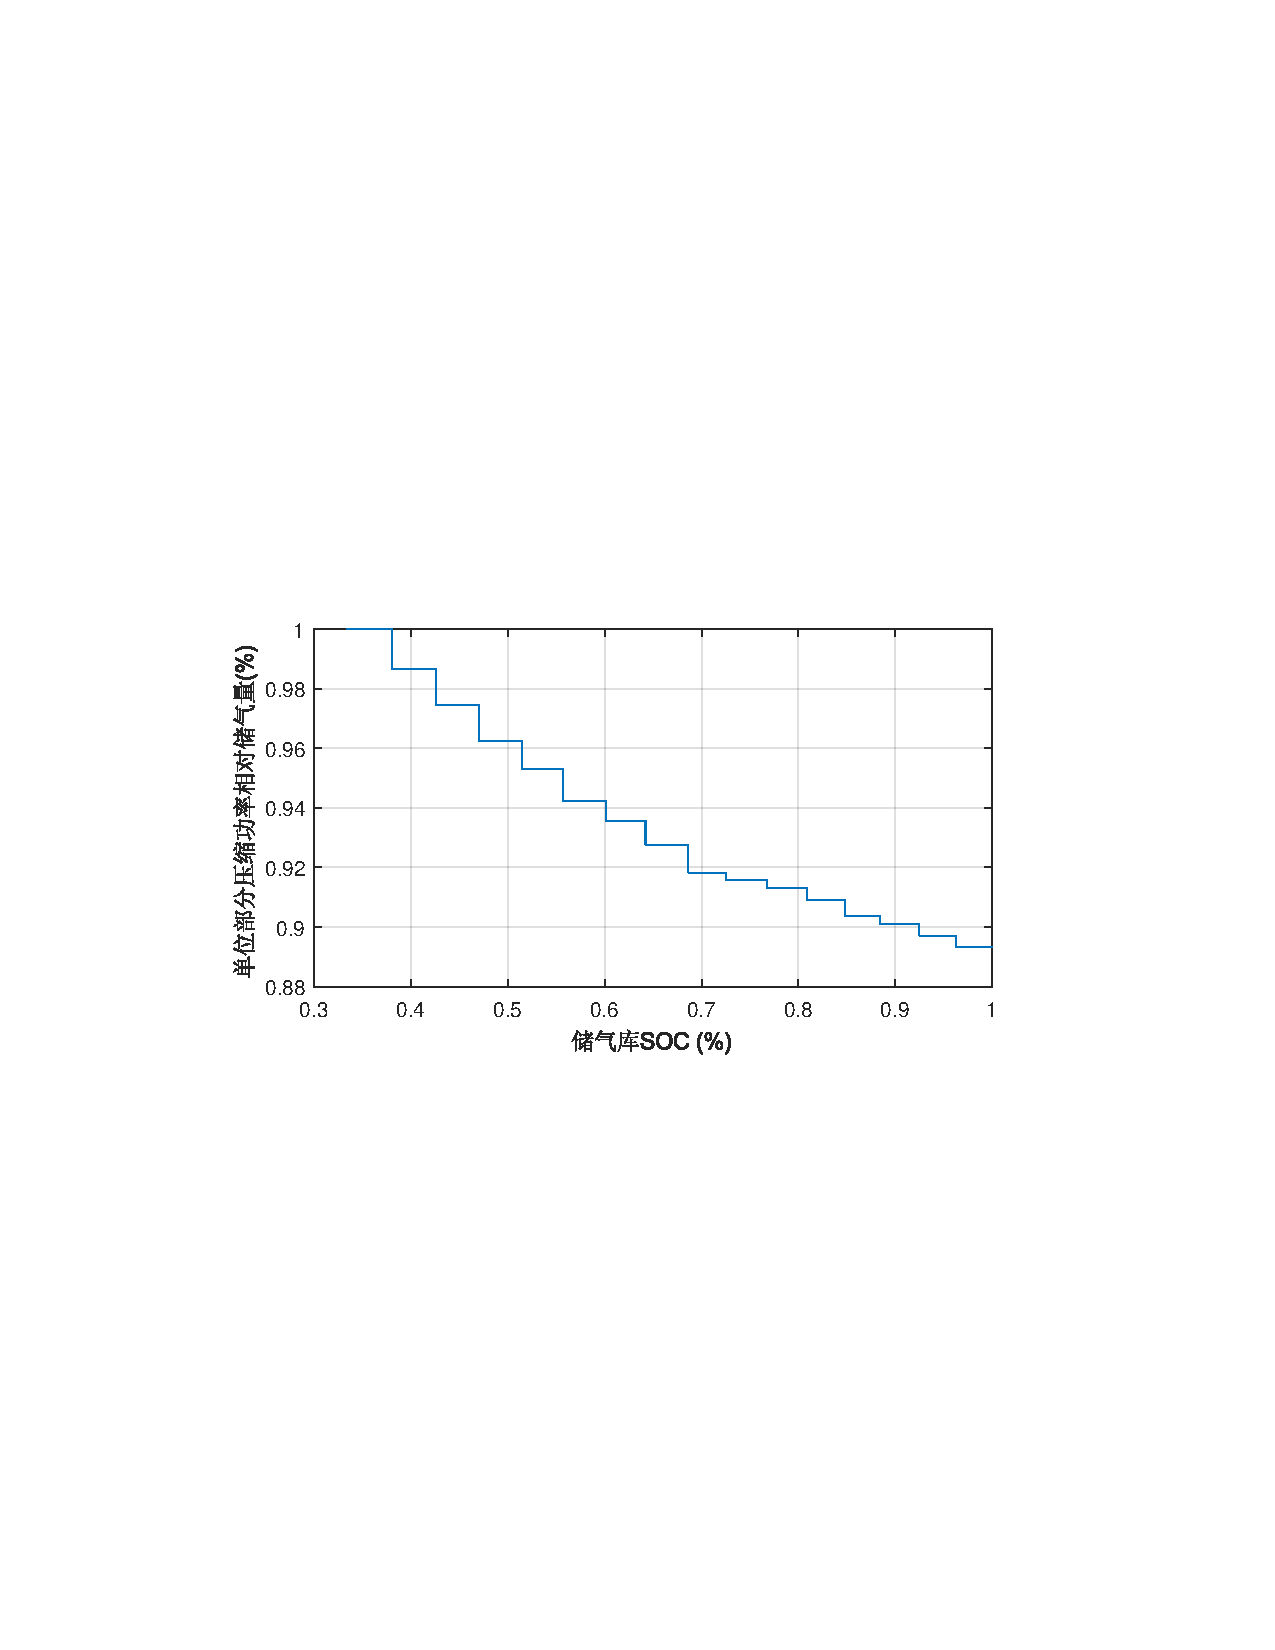
\includegraphics[scale=0.80]{figures/Chap1-8-Compression-SOC-Part-Load.pdf}
  \caption{不同储能水平单位压缩功率(MW)储能量}
  \label{fig:Compression-SOC-Part-Load}
\end{figure}

AA-CAES储能电站在膨胀释能过程中存在与D-CAES电站类似的特性,但相比D-CAES电站而言,AA-CAES电站用压缩储能阶段收集的空气压缩热能代替燃料补燃,其储能水平由储气库储气水平(决定透平入口空气压力)与储热罐储热水平(影响透平入口空气温度)同时决定。由第~\ref{sec:part-load-energy-he}节分析可知,压缩储能阶段收集的压缩热能受换热器的部分负载特性影响明显,从而导致AA-CAES电站释能发电环节的运行灵活性稍低于D-CAES电站。为将组件级的部分负载运行特性嵌入AA-CAES 系统级的宽工况运行模型,需要准确刻画各组件的部分负载运行特性对AA-CAES内部压力势能与压缩热能的存储与消耗水平的集中影响。

\subsection{内部势能-热能双能流耦合关系}
由第\ref{sec:part-load-energy}节中压缩机的部分负载热力学模型(\ref{equ:comp-real-temp-2})-(\ref{equ:comp-mid-var-2})及储气库的热力学动态模型(\ref{equ:Air-tank-model-G})可知,压缩功率对储气库的影响是通过注入空气增加储气量(空气压力势能),膨胀功率对储气库的影响是通过消耗空气减少储气量。另一方面,存储压缩热能的储热系统与压缩侧(或膨胀侧)的耦合来源于压缩侧(或膨胀侧)的换热器。因此,我们可以从换热器与压缩机(或膨胀机)间的热力学耦合关系来建立AA-CAES内部空气压力势能与压缩热能间的解耦存储与耦合释能关系。

本文以压缩储能过程中内部空气势能与压缩热能双能流间的解耦存储关系为例进行分析,膨胀释能过程中内部压力势能与压缩热能间的耦合释能关系与之类似。由式(\ref{equ:turb-power-all})可知,压缩机消耗的功率由空气质量流率及压缩机的入口与出口空气温度决定;由式(\ref{eq:he-comp-temp-out})可知,换热器的换热量由换热器入口与出口温度及质量流率决定。另一方面,储热量由换热器收集或消耗的热功率决定,为此只要合理刻画压缩机耗功与换热器收集的热功率间的关系即可建立内部空气压力势能与空气压缩热能间的解耦存储关系。

为了给出设计工况下压缩机(电)功率与换热器(热)功率间的量化关系,我们暂时假定换热器换热充分,每级压缩机入口空气温度相同(如文献\inlinecite{TICC-15,TICC-16}中的试验系统),考虑到压缩机出口温度等于相邻换热器入口温度(参见图~\ref{fig:CAES-thermal-struc} 所示~AA-CAES~结构及边界条件),从而换热器的换热功率大致等于压缩机消耗的电功率(亦可参见\ref{sec:chap2-bound-measure}节中的仿真分析)\footnote{出现压缩机耗功与换热器收集热功率相等现象的一个原因是,一般假定空气的定压比热容为定值,实际中二者并不相同。}。实际运行过程中,由于受组件部分负载特性及系统宽工况运行要求的影响,压缩机的电功率与储热系统的储热功率(换热器的集热功率)间的关系是时变的,同时还受AA-CAES系统本身结构参数以及运行方式的影响。因此,AA-CAES内部压力势能与压缩热能间的解耦存储与耦合释能关系可分别通过压缩侧与膨胀侧换热器的特性表示为
\begin{subequations}
\label{equ:coup-heat-power}
\begin{gather}
\varphi ({P_t^c,h_t^c}) = 0 \label{equ:coup-heat-power-char}\\
\phi ({P_t^d,h_t^d}) = 0 \label{equ:coup-heat-power-disc}
\end{gather}
\end{subequations}
其中,$P_t^c$与$P_t^d$分别为时段$t$(所有)压缩机消耗与(所有)膨胀机输出的电功率,实际上其值分别与第\ref{cha:simulation}章中对应时刻的压缩机耗功$W_{c}$ 与膨胀机输出功$W_{e}$ 相同\footnote{第2章针对压缩机、膨胀机及换热器等建立稳态热力学仿真模型时并未明确引入时间下标$t$,从本章开始我们将研究含第2章中各通用组件的AA-CAES不同实现或应用形式在电力系统中的运行建模、调度运行及市场运营等问题,相应模型一般会直接在第2章相关变量的基础上加入时间下标$t$,而不做过多解释。 同时,我们假定一个运行时段内各个时刻各物理量不发生变化,而时段的大小视所分析问题的不同而有所差别。此外,在不引起混淆的情况下,我们允许对时刻与时段的混用。};$h_t^c$ 与$h_t^d$ 分别为储能阶段注入储热系统的热功率与释能阶段消耗的热功率,实际上其值可由第\ref{cha:simulation}章中的HTF比热容$c_p^{HTF}$,质量流率($\dot m_e^{HTF}$,$\dot m_c^{HTF}$),以及对应的HTF温度($T^{TES}, T_{c,HX}^{HTF, Merge}, T_{e,HX}^{Merge},T_{cool}^{HTF}$)等计算而得。(\ref{equ:coup-heat-power-char})表示储能过程中储热功率与储电功率(即压缩机电功率)间的耦合关系,间接刻画了压力势能与压缩热能的解耦存储关系;(\ref{equ:coup-heat-power-disc}) 表示释能过程中耗热功率与放电功率(即膨胀机电功率)间的耦合关系,间接刻画了压力势能与压缩热能的耦合释能关系。

特别地,势能与热能双能流间耦合关系(\ref{equ:coup-heat-power})的特殊形式可表示为
\begin{subequations}
\label{equ:coup-heat-power-spe}
\begin{gather}
h_t^c = \varphi ({P_t^c})P_t^c \label{equ:coup-heat-power-char-spe}\\
P_t^d = \phi ({P_t^d})h_t^d  \label{equ:coup-heat-power-disc-spe}
\end{gather}
\end{subequations}
其中,$\varphi ({P_t^c})$与$\phi ({P_t^d})$分别为储能过程与释能过程中所有换热器部分负载运行时的集中(等效)效能,也分别表征了AA-CAES 压缩储能过程中将电功率转化为热功率以及膨胀释能过程中将热功率转化为电功率的能力,与热泵等电热转换设备的效率具有类似的物理意义。

本章后续使用$P_t^c$与$P_t^d$表征AA-CAES与电力系统的(电)功率输入与(电)功率输出接口,实现对$W_c$与$W_e$及压缩机与膨胀机内部热力学特性的封装;同时,也采用$h_t^c$ 与$h_t^d$ 实现对内部HTF热力学状态相关信息的封装。通过引入隐函数$\varphi ({P_t^c,h_t^c})$与$\phi ({P_t^d,h_t^d})$,我们将第2章中复杂的压力势能与压缩热能间的热力学耦合关系集中体现于$\varphi(\cdot) $与$\phi(\cdot)$上,后续应用只需关注接口信息($ P_t^c$、$P_t^d$、$h_t^c$、 $h_t^d$)以及$\varphi(\cdot)$与$\phi(\cdot)$ 的具体形式即可。换言之,给定任一外部应用的可行功率接口信息,AA-CAES便能通过(外部无需了解的)内部的热力学状态参数实现该功率接口。

\subsection{外部电功率与储/耗气量的耦合关系}
AA-CAES组件的部分负载特性对储气库储气水平的整体影响表现在式(\ref{equ:air-SOC-energy})中压缩功率(或膨胀功率)受背压(或入口压力)影响导致的单位压缩(或膨胀)电功率储气量(或耗气量)的部分负载特性。为此,本文用$m_t^{ch}$ 与$m_t^{dis}$ 分别表示计及压缩机与膨胀机的部分负载特性时,时段$t$ 进入与流出储气库的高压空气质量,且满足:
\begin{subequations}
\label{equ:coup-mass-SOC}
\begin{gather}
m_t^{ch} = \Gamma({P_t^c,A_t^{soc}})P_t^c\label{equ:coup-mass-SOC-char}\\
m_t^{dis} = \Psi({P_t^d,A_t^{soc}})P_t^d \label{equ:coup-mass-SOC-disc}
\end{gather}
\end{subequations}
其中,$A_t^{soc}$ 为储气库无量纲储气水平;函数$\Gamma(\cdot)$ 建立了储能过程中压缩功率$P_t^c$ 与进气量$m_t^{ch}$间的关系;函数$\Psi(\cdot)$ 建立了释能过程中膨胀功率$P_t^d$与耗气量$m_t^{dis}$间的关系,即函数$\Gamma (\cdot)$与$\Psi(\cdot)$分别等效表征了单位压缩功率的进气量与单位膨胀功率的耗气量,反映了压缩机与膨胀机的部分负载运行特性与储气库动态特性间的耦合关系。

一般地,函数$\Gamma(\cdot)$与函数$\Psi(\cdot)$的具体表达式依赖于第\ref{cha:simulation}章中引入的AA-CAES的四种运行模式,即定压-定压、定压-滑压、滑压-定压、滑压- 滑压等。以函数$\Gamma(\cdot)$为例,当不存在储气库入口侧节流阀(见\ref{fig:CAES-thermal-struc}),即压缩侧采用滑压运行策略时,压缩储能过程中压缩机的背压为储气库实时压力,函数$\Gamma(\cdot)$ 与$A_t^{soc}$有关;当存在入口侧节流阀,即压缩机采用定压运行策略时,压缩机的部分负载运行特性不受储气库压力影响,函数$\Gamma(\cdot)$ 退化为$\Gamma (P_t^c)$ ,与$A_t^{soc}$ 无关。特别地,当AA-CAES处于额定工况运行,且储气库入口与出口均存在节流阀(定压-定压运行)时,$\Gamma(\cdot)$与$\Psi(\cdot)$变为固定系数,式(\ref{equ:coup-mass-SOC})将退化为常效率模型。由此可见,外部输入/输出电功率与储气库进/出气量间的通用耦合关系(\ref{equ:coup-mass-SOC})涵盖了AA-CAES系统的典型运行模式。

\subsection{热力学特性曲线簇}
基于前述分析,储能电站运行时的AA-CAES系统级的宽工况特性,可由基于换热器视角表示的内部势能-热能双能流耦合关系函数$\varphi$与$\phi$,以及基于压缩机与膨胀机视角表示的外部输入/输出电功率与储气/耗气量间耦合关系的函数$\Gamma $与$\Psi$集中表示\cite{CAES-Wind-Rui-19}。本文将($\Gamma$, $\Psi$, $\varphi$, $\phi$)称为表征AA-CAES宽工况运行特性的热力学特性曲线簇,即AA-CAES对外部应用提供的接口函数,其可基于第\ref{cha:simulation}章中计及组件部分负载特性的AA-CAES宽工况热力学仿真模型产生,或由实际AA-CAES储能电站的运行数据拟合给定\cite{CAES-Wind-Rui-19}。其理性在于,电力系统调度等应用处理火电机组的复杂运行特性时,一般会采用常系数(未考虑火电机组宽工况特性)或采用基于输入输出特性曲线的变系数,而该特性曲线通常由火电厂实测运行数据拟合给定\cite{CAES-Wind-Rui-19}。在实际运行过程中,热力学特性曲线簇($\Gamma$, $\Psi$, $\varphi$, $\phi$)中的函数$\Gamma(\cdot)$与$\Psi(\cdot)$受AA-CAES储能电站运行模式的影响,而函数$\varphi(\cdot)$与$\phi(\cdot)$则受供能模式影响。
%以下基于第2章的仿真系统给出该特性曲线簇的典型形状。

%\subsection{仿真参数设置}
%本节采用图~\ref{fig:CAES-thermal-struc}所示的两级压缩两级膨胀~AA-CAES~储能电站,以典型滑压-定压运行模式分析宽工况热力学特性曲线,为面向智能电网应用的~AA-CAES~构建不失建模准确性的能量及备用模型提供基础。本节以江苏金坛~60~MW AA-CAES储能电站设计参数\footnote{部分参数细节与实际参数有所出入,但不影响本章建模的思路。}为例,进行分析。

%\begin{table}[htb]
%  \centering
%  \begin{minipage}[t]{0.70\linewidth} % 如果想在表格中使用脚注,minipage是个不错的办法
%  \caption{60MW AA-CAES 储能电站空气压缩机额定参数}
%  \label{tab:CAES-60-para-comp}
%    \begin{tabularx}{\linewidth}{ccccccc}
%      \toprule[1.5pt]
%      \multirow{2}*{\heiti 压缩级} &  \multirow{2}*{\heiti 增压比} &  \multirow{2}*{\heiti 绝热效率(\%)} &  \multicolumn{2}{c}{\heiti 压力(Mpa)} & \multicolumn{2}{c}{\heiti 温度($^{\circ}$C)}\\
%      \cline{4-7}
%        &   &   &  进气 & 排气 & 进气 & 排气 \\
%     \midrule[1pt]
%      一级 & 3.545 & 72.8 & 0.099 & 0.351  & 25 & 143 \\
%      二级 & 2.668 & 78.6 & 0.351 & 0.913  & 45 & 145 \\
%      三级 & 2.677 & 82.2 & 0.913 & 2.392  & 45 & 149 \\
%      \bottomrule[1.5pt]
%    \end{tabularx}
%  \end{minipage}
%\end{table}

%\begin{table}[htb]
%  \centering
%  \begin{minipage}[t]{0.75\linewidth} % 如果想在表格中使用脚注,minipage是个不错的办法
%  \caption{60MW AA-CAES储能电站空气透平膨胀机额定参数}
%  \label{tab:CAES-60-para-turb}
%    \begin{tabularx}{\linewidth}{ccccccc}
%      \toprule[1.5pt]
%      \multirow{2}*{\heiti 膨胀级} &  \multirow{2}*{\heiti 膨胀比} &  \multirow{2}*{\heiti 绝热效率(\%)} &  \multicolumn{2}{c}{\heiti 压力(Mpa)} & \multicolumn{2}{c}{\heiti 温度($^{\circ}$C)}\\
%      \cline{4-7}
%        &   &   &  进气 & 排气 & 进气 & 排气 \\
%     \midrule[1pt]
%      一级 & 3.545 & 87.9 & 3.00 & 1.02  & 100 & 12 \\
%      二级 & 2.668 & 87.0 & 1.01 & 0.34  & 100 & 13 \\
%      \bottomrule[1.5pt]
%    \end{tabularx}
%  \end{minipage}
%\end{table}
%
%\begin{table}[htb]
%  \centering
%  \begin{minipage}[t]{0.85\linewidth} % 如果想在表格中使用脚注,minipage是个不错的办法
%  \caption{60MW AA-CAES 储能电站压缩侧换热器额定参数}
%  \label{tab:CAES-60-para-he-comp}
%    \begin{tabularx}{\linewidth}{cccccccc}
%      \toprule[1.5pt]
%      \multirow{2}*{\heiti 换热级} &  \multicolumn{2}{c}{\heiti 空气温度($^{\circ}$C)} &  \multicolumn{2}{c}{\heiti 冷却水温度($^{\circ}$C)}  & \multicolumn{2}{c}{\heiti 温差($^{\circ}$C)} & \multirow{2}*{\heiti 水侧流量(kg/h)}\\
%      \cline{2-7}
%        &  入口 & 出口  & 入口 & 出口  & 热端  & 冷端 &   \\
%     \midrule[1pt]
%      一级 & 143 & 45 & 35 & 120  & 23 & 10  & 451.091\\
%      二级 & 145 & 45 & 35 & 120  & 25 & 10 & 462.841\\
%      三级 & 149 & 45 & 35 & 120  & 29 & 10 & 487.968 \\
%      \bottomrule[1.5pt]
%    \end{tabularx}
%  \end{minipage}
%\end{table}
%
%\begin{table}[htb]
%  \centering
%  \begin{minipage}[t]{0.85\linewidth} % 如果想在表格中使用脚注,minipage是个不错的办法
%  \caption{60MW AA-CAES 储能电站膨胀侧换热器额定参数}
%  \label{tab:CAES-60-para-he-turb}
%    \begin{tabularx}{\linewidth}{cccccccc}
%      \toprule[1.5pt]
%      \multirow{2}*{\heiti 换热级} &  \multicolumn{2}{c}{\heiti 空气温度($^{\circ}$C)} &  \multicolumn{2}{c}{\heiti 加热水温度($^{\circ}$C)}  & \multicolumn{2}{c}{\heiti 温差($^{\circ}$C)} & \multirow{2}*{\heiti 水侧流量(kg/h)}\\
%      \cline{2-7}
%        &  入口 & 出口  & 入口 & 出口  & 热端  & 冷端 &   \\
%     \midrule[1pt]
%      一级 & -10 & 100 & 120 & 35  & 20 & 45  & 2841\\
%      二级 & 12  & 100 & 120 & 35  & 20 & 23  & 2212\\
%      三级 & 13  & 100 & 120 & 35  & 20 & 23  & 2169\\
%      \bottomrule[1.5pt]
%    \end{tabularx}
%  \end{minipage}
%\end{table}

\section{宽工况双SOC建模框架及典型模型}
\label{sec:dual-SOC}
前已提及,第~\ref{cha:simulation}章建立的宽工况热力学仿真模型主要用于热力学特性分析,若直接用于电力系统中AA-CAES储能电站的运行分析,将导致模型异常复杂,不便于实际工程所采纳。本节在第\ref{sec:chap3-aa-caes-sim}节提出的宽工况热力学特性曲线簇的基础上,借鉴电池储能的荷电水平(State-of-charge,SOC)建模思想,将
从能量转换类模块(压缩机与空气透平)及能量转移类模块(换热器)视角得出的热力学特性曲线簇“嵌入”内部能量存储类模块(储气库与储热罐)的SOC方程中,建立面向电力系统应用的AA-CAES宽工况双SOC建模体系及具体模型,其基本框架如图~\ref{fig:AA-CAES-Part-Load-Model}所示。

\begin{figure}[H] % use float package if you want it here
  \centering
  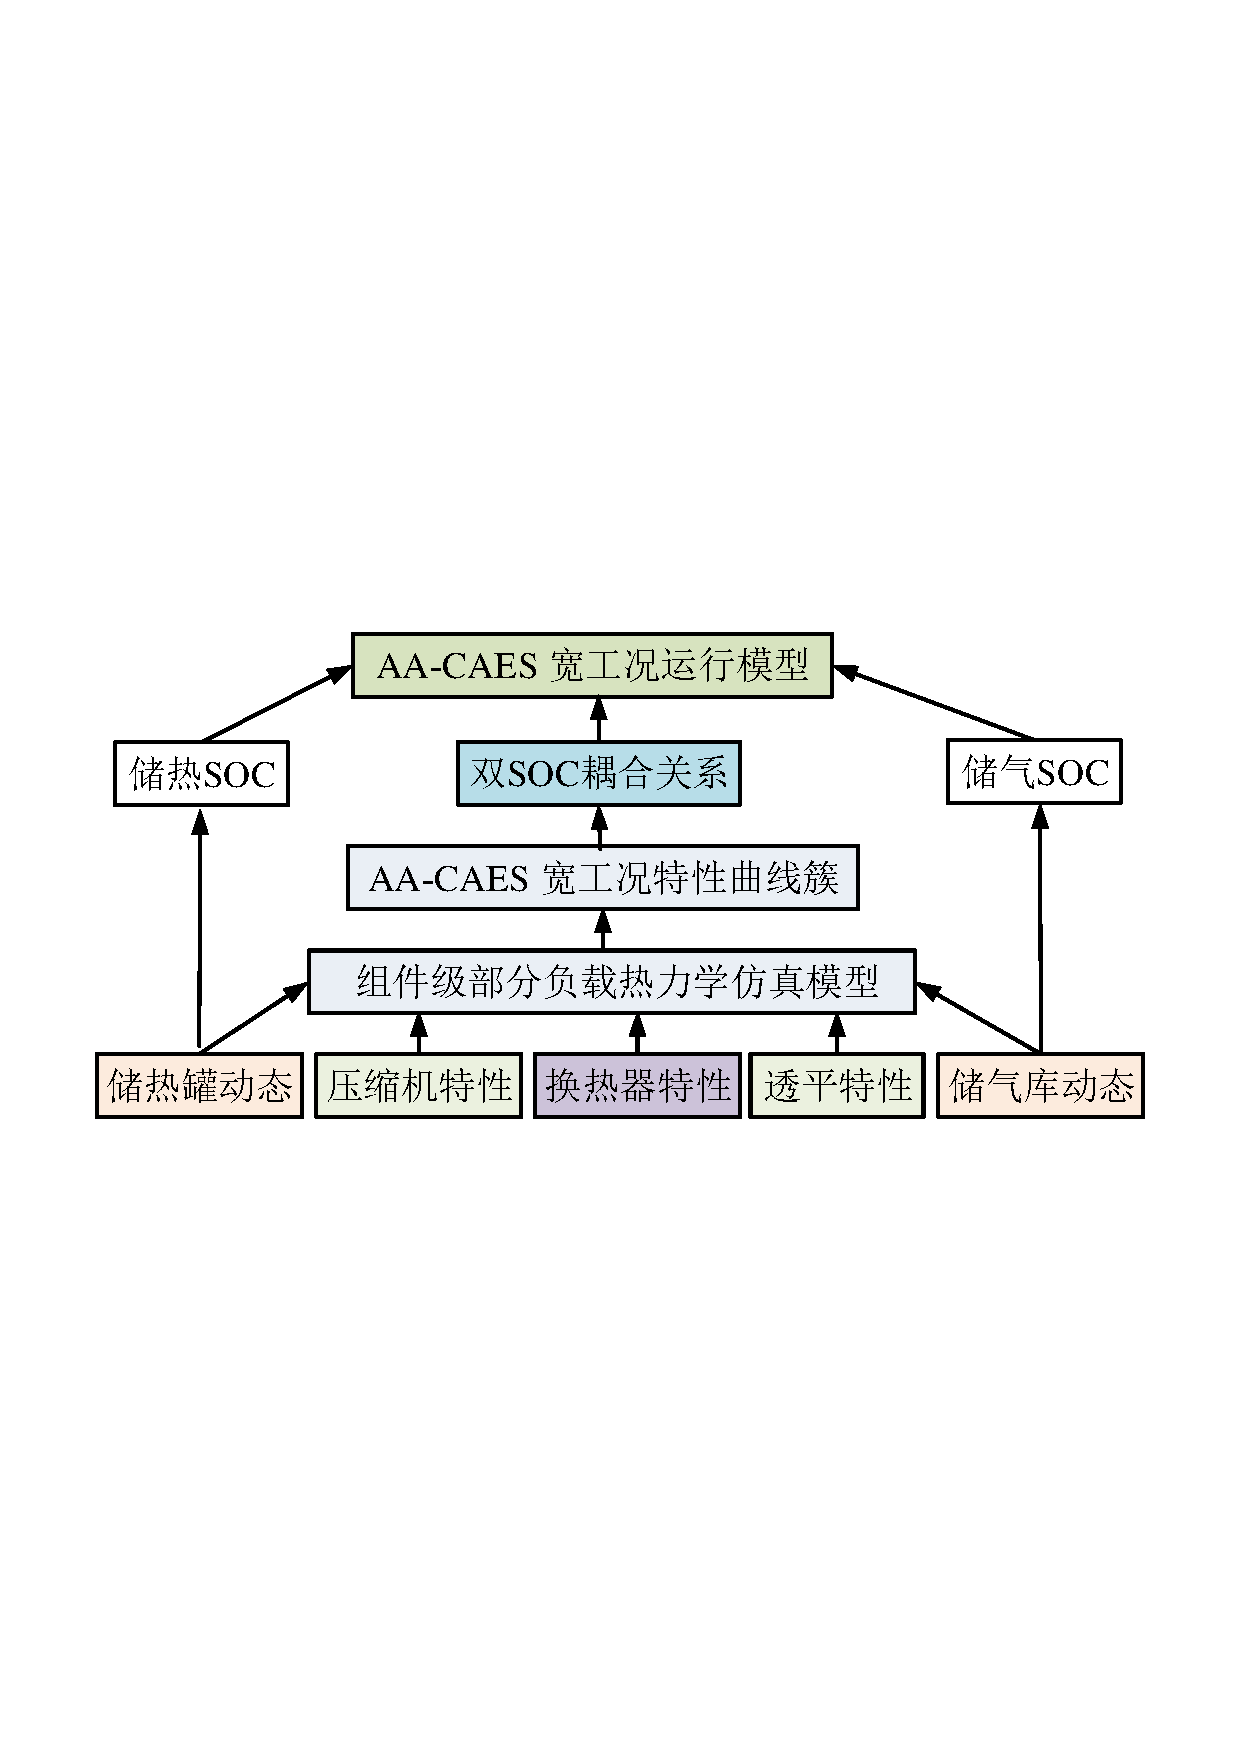
\includegraphics[scale=0.60]{figures/Chap3-2-AA-CAES-Part-Load-Model.pdf}
  \caption{AA-CAES储能电站的双SOC模型建模框架}
  \label{fig:AA-CAES-Part-Load-Model}
\end{figure}

运用双SOC模型建模框架,我们可以得出面向电力规划、调度运行及市场运营等应用的AA-CAES储能电站的系列模型。本节将重点给出双SOC能量模型、双SOC能量与备用模型,以及能量与备用模型的扩展形式,以说明宽工况双SOC建模框架的应用方法。

\subsection{双SOC能量模型}
\label{sec:dual-SOC-energy}
一般地,储气库的储气SOC可以采用储气压力构建,如文献\inlinecite{CAES-IES-16-Rui}中采用的储气库模型。 然而,基于压力动态描述的储气SOC模型难以将第
\ref{cha:simulation}章中给出的面向AA-CAES热力学特性仿真的通用储气库、等温储气库及绝热储气库等模型纳入统一框架。换言之,采用不同的储气库仿真模型时,影响储气库压力动态的因素不同,采用G模型时储气库压力受进/出气量以及储气库内空气与周围环境传热过程的影响;采用VT与VA模型时,压力动态仅受进/出空气的热力学状态影响。

本节基于储气库中的空气质量动态建立储气SOC模型,其出发点在于,不论储气库采用G模型、VT或VA模型,质量动态方程仅受进/出气量影响,且具有简洁统一的形式(参见
(\ref{equ:Air-tank-model-G})、(\ref{equ:Air-tank-model-VT})、(\ref{equ:Air-tank-model-VA})),%(可参见(\ref{equ:Air-tank-model-G-M})、(\ref{equ:Air-tank-model-VT-M}) 及(\ref{equ:Air-tank-model-VA-M})),
同时也便于与第\ref{sec:chap3-aa-caes-sim}节中的宽工况特性曲线簇实现有机结合。事实上,针对传统D-CAES电站,基于储气库空气质量构建储气SOC的思路已被逐渐接受,如文献\inlinecite{CAES-Bilinear-17,CAES-Reserve-Bid-Therm-16}。

基于储气库热力学动态模型(\ref{equ:Air-tank-model-G})-(\ref{equ:Air-tank-model-VA}),可将储气SOC表示为\cite{CAES-Wind-Rui-19}
\begin{subequations}
\label{equ:air-SOC-energy}
\begin{gather}
A_{t + 1}^{soc} = A_t^{soc}(1-\gamma_{A}) + \frac{1}{{{A_{\max}^{circ}}}}({m_t^{ch} - m_t^{dis}})\label{equ:air-SOC-energy-balance}\\
A_{\min }^{soc} \le A_t^{soc} - \frac{{m_t^{dis}}}{{{{\rm{A}}_{\max }^{circ}}}}\\
{\rm{A}}_t^{soc} + \frac{{m_t^{ch}}}{{{{\rm{A}}_{\max }^{circ}}}} \le A_{\max }^{soc}
\end{gather}
\end{subequations}
其中,$\gamma_{A}$为表征储气库漏气特性的常数,一般可设为0-0.02,基于第2章不计及储气库漏气问题的假设,此处取为0;${A_{\max}^{circ}}$ 为储气库最大循环空气质量,由储气库压力上下限($p_{as}^{min}$, $p_{as}^{max}$) 及体积$V_{as}$等决定;${{A}}_t^{soc}$ 为时刻$t$的储气百分数;${{A}}_{\min }^{soc}$ 与 ${{A}}_{\max }^{soc}$ 分别为维持最小与最大储气压力所需的空气质量百分数。
 %$m_t^{ch}$ 与$m_t^{dis}$分别表示进入与流出储气库的空气质量,受宽工况运行影响。由第~\ref{sec:chap3-aa-caes-sim}节分析可知,宽工况运行模式下,AA-CAES储能电站单位压缩功率对应的 $m_t^{ch}$ 将减小,单位膨胀功率所需的$m_t^{dis}$ 将增大。

类似地,基于储热系统的热力学动态模型(\ref{equ:TES-HTF-temp}),可将储热SOC表示为\footnote{若需考虑AA-CAES对外的供热功率(假定用收集的压缩热供热),只需在(\ref{equ:TES-SOC-energy-balance})中新增一项$h_t^{g}$即可。}\cite{CAES-Wind-Rui-19}
\begin{subequations}
\label{equ:TES-SOC-energy}
\begin{gather}
H_{t + 1}^{soc} = H_t^{soc}(1-\gamma_{H}) + \frac{1}{{{H_{\max}^{circ}}}}({h_t^c\Delta t - h_t^d\Delta t})\label{equ:TES-SOC-energy-balance}\\
H_{\min }^{soc} \le H_t^{soc} - \frac{{h_t^d\Delta t}}{{{H_{\max }^{circ}}}}\\
H_t^{soc} + \frac{{h_t^c\Delta t}}{{{H_{\max }^{circ}}}} \le H_{\min }^{soc}
\end{gather}
\end{subequations}
其中, $\gamma_{H}$表征储热罐与周围环境的换热过程引起的储热量损耗,其大小与储热罐特性有关,可假定为常数,当储热罐采用绝热模型时,其值为0;${H_{\max}^{circ}}$ 为储热系统最大储热量,一般需根据应用场景进行设置,如热电联供模式下的最大储热量比仅供电模式要大;$H_t^{soc}$为储热相对百分数;${{H}}_{\min }^{soc}$与${{H}}_{\max }^{soc}$ 分别为最小与最大储热百分数;$\Delta t$ 为时间间隔,其它参数物理意义与式(\ref{equ:air-SOC-energy})类似。

在AA-CAES储能电站的压缩储能过程中,通过压力势能与压缩热能的解耦存储,压缩功率同时改变储气SOC与储热SOC的状态;膨胀释能过程中,通过压力势能与压缩热能的耦合释能,储气SOC与储热SOC共同影响膨胀功率\cite{CAES-Wind-Rui-19}。因此,通过引入含有压缩功率与膨胀功率接口的宽工况热力学特性曲线簇($\Gamma$, $\Psi$, $\varphi$, $\phi$),即可实现储气SOC与储热SOC的耦合\cite{CAES-Wind-Rui-19}。

综上,AA-CAES储能电站的宽工况双SOC能量模型由(\ref{equ:coup-heat-power})、(\ref{equ:coup-mass-SOC})、(\ref{equ:air-SOC-energy})及(\ref{equ:TES-SOC-energy})构成,其对电力系统调度等外部应用提供了功率接口($P_t^c$, $P_t^d$)以及储能水平($A_t^{soc}$, $H_t^{soc}$)。

\subsection{双~SOC~能量与备用模型}
\label{sec:dual-SOC-Reserve}

在第\ref{sec:dual-SOC-energy}节中我们建立了AA-CAES储能电站的宽工况双SOC能量模型。事实上,AA-CAES储能电站可为电网提供容量备用等灵活性支撑。为此,可将双SOC 能量模型扩展为计及备用特性的双~SOC~能量与备用模型。我们仅考虑正负荷备用\footnote{该设定的合理性主要体现在系统中备用主要是用于缓解调峰或机组/线路临时故障退出引起的负荷难以满足等问题。},即通过减少压缩机消耗的电功率$P_t^c$与增加透平输出的电功率$P_t^d$来提供灵活性支撑。由图\ref{fig:CAES-AS-Overview} 分析可知,压缩储能过程能提供旋转备用$P_t^{c,sr}$,膨胀释能过程可同时提供旋转备用$P_t^{d,sr}$ 与非旋转备用$P_t^{d,nr}$。为了刻画AA-CAES的备用容量接口,我们定义如下的等效压缩功率与等效膨胀功率,即
\begin{subequations}
\label{equ:def-Pc-Pd-eq}
\begin{gather}
P_t^{c,eq} = P_t^c - P_t^{c,sr}\label{equ:def-Pc-eq}\\
P_t^{d,eq} = P_t^d + P_t^{d,sr} + P_t^{d,nr}\label{equ:def-Pd-eq}
\end{gather}
\end{subequations}
其中,$P_t^{c,eq}$表示计及压缩机的旋转备用容量的等效压缩功率;$P_t^{d,eq}$表示计及空气透平旋转备用及非旋转备用容量的等效膨胀功率。

计及备用特性后,储气SOC模型可调整为
\begin{subequations}
\label{equ:air-SOC-reserve}
\begin{gather}
A_{t + 1}^{soc} = A_t^{soc}(1-\gamma_A) + \frac{1}{{{A_{\max }^{circ}}}}({m_t^{ch} - m_t^{dis}})\\
A_{\min }^{soc} \le A_t^{soc} - \frac{{m_t^{dis,eq}}}{{{A_{\max}^{circ}}}}\label{equ:air-SOC-reserve-diff}\\
{{A}}_t^{soc} + \frac{{m_t^{ch}}}{{{{\rm{A}}_{\max}^{circ}}}} \le A_{\max }^{soc}
\end{gather}
\end{subequations}
相应地,储热SOC模型可调整为\footnote{若需考虑AA-CAES热电联供时具有的热功率备用能力,只需稍微修改(\ref{equ:TES-SOC-reserve})即可。}
\begin{subequations}
\label{equ:TES-SOC-reserve}
\begin{gather}
H_{t + 1}^{soc} = H_t^{soc}(1-\gamma_H) + \frac{1}{{{H_{\max}^{circ}}}}({h_t^c\Delta t - h_t^d\Delta t})\label{equ:TES-SOC-reserve-S1}\\
H_{\min }^{soc} \le H_t^{soc} - \frac{{h_t^{d,eq}\Delta t}}{{{H_{\max}^{circ}}}}\label{equ:TES-SOC-reserve-diff}\\
H_t^{soc} + \frac{{h_t^c\Delta t}}{{{H_{\max}^{circ}}}} \le H_{\max }^{soc}
\end{gather}
\end{subequations}
其中,$m_t^{dis,eq}$与$h_t^{d,eq}$分别为对应于等效膨胀功率$P_t^{d,eq}$的耗气量与耗热功率,二者分别满足:
\begin{subequations}
\label{equ:coup-mass-heat-SOC-reserve}
\begin{gather}
m_t^{dis,eq} = \Psi ({P_t^{d,eq},A_t^{soc}})P_t^{d,eq}\label{equ:coup-mass-SOC-reserve-S3}\\
\phi ({P_t^{d,eq},h_t^{d,eq}}) = 0\label{equ:coup-heat-power-reserve-S3}
\end{gather}
\end{subequations}

需要强调的是,在双SOC能量与备用模型中的储气及储热SOC与双SOC能量模型的储气及储热SOC的不同之处仅在于(\ref{equ:air-SOC-reserve-diff})与(\ref{equ:TES-SOC-reserve-diff}),其原因在于不计及备用容量的实际调用时,备用容量只受到储气与储热SOC的上下界影响,而不影响储气SOC与储热SOC方程。在膨胀释能过程中,提供备用容量时需要增大膨胀功率,其备用容量受到储气量下限及储热量下限的影响;在压缩储能过程中,提供备用容量时由于需要减小压缩功率,备用容量不受储气量上限与储热量上限的影响。

综上,AA-CAES储能电站的宽工况双SOC能量与备用模型由(\ref{equ:coup-heat-power})、(\ref{equ:coup-mass-SOC})、(\ref{equ:def-Pc-Pd-eq})、(\ref{equ:air-SOC-reserve})、(\ref{equ:TES-SOC-reserve})及(\ref{equ:coup-mass-heat-SOC-reserve})组成,其对外部电力系统应用提供了功率接口($P_t^c$,$P_t^d$),容量备用接口($P_t^{c,sr}$,$P_t^{d,sr}$,$P_t^{d,nr}$),以及储能水平($A_t^{soc}$, $H_t^{soc}$)。

\subsection{能量与备用模型的扩展}
\label{sec:dual-SOC-Reserve-exten}
第\ref{sec:dual-SOC-Reserve}节中所建的双~SOC~能量与备用模型中未考虑实际运行(或实时市场)中备用调度对AA-CAES 储能电站双SOC状态的影响,一般用于含储能的电力系统灵活性评估或容量规划、不计及备用调用的储能电站市场运营等问题。本节旨在进一步扩展双~SOC~能量与备用模型,以计及备用容量的调用对储气与储热SOC状态的影响。

为刻画计及备用容量的实际调用时,AA-CAES的双SOC模型接口,我们定义计及备用调用的等效压缩功率与等效膨胀功率,即
\begin{subequations}
\label{equ:def-power-relation}
\begin{gather}
P_t^{c,Ev} = P_t^c - P_t^{c,sr}u_t^{sr}\\
P_t^{d,Ev} = P_t^d + P_t^{d,sr}u_t^{sr} + P_t^{d,nr}u_t^{nr}
\end{gather}
\end{subequations}
其中,$u_t^{sr}$与$u_t^{nr}$分别为表征旋转备用与非旋转备用容量调用状态的布尔量;$P_t^{c,Ev}$为计及备用容量调用($P_t^{c,sr}$)的等效压缩功率;$P_t^{d,Ev}$为计及备用容量($P_t^{d,sr}$,$P_t^{d,nr}$)调用的等效膨胀功率。


计及备用调用后,储气SOC模型可修正为
\begin{subequations}
\label{equ:air-SOC-reserve-exten}
\begin{gather}
A_{t + 1}^{soc} = A_t^{soc}(1-\gamma_A) + \frac{1}{{{A_{\max}^{circ}}}}({m_t^{ch,Ev} - m_t^{dis,Ev}})\\
A_{\min }^{soc} \le A_t^{soc} - \frac{{m_t^{dis,Ev}}}{{{A_{\max}^{circ}}}}\\
{\rm{A}}_t^{soc} + \frac{{m_t^{ch}}}{{{{\rm{A}}_{\max}^{circ}}}} \le A_{\max }^{soc}
\end{gather}
\end{subequations}
相应地,储热SOC模型可修正为
\begin{subequations}
\label{equ:TES-SOC-reserve-exten}
\begin{gather}
H_{t + 1}^{soc} = H_t^{soc}(1-\gamma_H) + \frac{1}{{{H_{\max}^{circ}}}}({h_t^{c,Ev}\Delta t - h_t^{d,Ev}\Delta t})\\
H_{\min }^{soc} \le H_t^{soc} - \frac{{h_t^{d,Ev}\Delta t}}{{{H_{\max}^{circ}}}}\\
H_t^{soc} + \frac{{h_t^c\Delta t}}{{{H_{\max}^{circ}}}} \le H_{\max }^{soc}
\end{gather}
\end{subequations}
其中,$m_t^{ch,Ev}$与$m_t^{dis,Ev}$分别为等效压缩功率$P_t^{c,Ev}$与等效膨胀功率$P_t^{d,Ev}$对应的进气量与耗气量;$h_t^{c,Ev}$与$h_t^{d,Ev}$分别为$P_t^{c,Ev}$与$P_t^{d,Ev}$对应的储热功率及耗热功率。特别地,计及备用容量的调用后,内部热力学特性间的耦合关系(宽工况特性曲线方程)需调整为
\begin{subequations}
\label{equ:coup-heat-power-reserve-exten}
\begin{gather}
m_t^{ch,Ev} = \Gamma ({P_t^{c,Ev},A_t^{soc}})P_t^{c,Ev}\\
m_t^{dis,Ev} = \Psi ({P_t^{d,Ev},A_t^{soc}})P_t^{d,Ev}\\
\varphi ({P_t^{c,Ev},h_t^{c,Ev}}) = 0\\
\phi ({P_t^{d,Ev},h_t^{d,Ev}}) = 0
\end{gather}
\end{subequations}

综上,计及备用调用后,AA-CAES储能电站双SOC能量与备用扩展模型由(\ref{equ:def-power-relation})、(\ref{equ:air-SOC-reserve-exten})、(\ref{equ:TES-SOC-reserve-exten})及(\ref{equ:coup-heat-power-reserve-exten})组成,其对外部电力系统应用提供了功率接口($P_t^c$,$P_t^d$)、容量备用接口($P_t^{c,sr}$,$P_t^{d,sr}$,$P_t^{d,nr}$)、储能水平($A_t^{soc}$, $H_t^{soc}$),以及备用容量在实际运行中的调用状态($u_t^{sr}$, $u_t^{nr}$)。

\section{计及AA-CAES宽工况特性的风-储协同调度运行}
\label{sec:chap3-wind-ESS-operation}
本节基于第\ref{sec:dual-SOC}节中储能电站的宽工况双SOC能量模型,分析AA-CAES的宽工况运行特性对风电与储能电站协同系统(如图\ref{fig:AA-CAES-Stru-Felixibity} 中配置方案)运行特性的影响。

\subsection{协同发电能力分析模型}
本节假定风- 储协同系统以最大化风电上网电量或风电容量因子(Capacity Factor, CF)为目标。除满足第\ref{sec:dual-SOC}节中的双SOC能量模型之外,风-储协同运行需满足如下的运行限制\cite{CAES-Wind-Rui-19}:
\begin{subequations}
\label{eq:WT-CAES-Power-Limit}
\begin{gather}
u_t^c + u_t^d \le 1,u_t^c,u_t^d \in \left\{ {0,1} \right\}, \forall t\\
P_{\min }^cu_t^c \le P_t^c \le P_{\max }^cu_t^c, \forall t \\
 P_{\min }^du_t^d \le P_t^d \le P_{\max }^du_t^d, \forall t
\end{gather}
\end{subequations}
其中,$u_t^c$ 与 $u_t^d$ 分别为表示压缩储能与膨胀释能运行状态的布尔量;$P_{\max }^c$ 与 $P_{\max }^d$ 分别为压缩机与空气透平的额定功率;$P_{\min }^c$ 与 $P_{\min }^d$ 分别为压缩机与空气透平的最小技术出力。对于AA-CAES储能电站这类宽工况运行特性较为明显的系统,最小技术出力的确定需通过经济性评估等界定,如火电机组按照机组容量的不同,大型机组的最小技术出力一般设定为额定功率的50\%。

为了聚焦于宽工况运行对风-储系统影响的分析,我们假定AA-CAES储能电站仅通过与之协同运行的风电进行储能(参见图\ref{fig:AA-CAES-Stru-Felixibity})。因此,风-储系统系统需满足如下约束:
\begin{equation}
\label{eq:WT-Power-Limit}
P_t^c \le {W_t},P_t^d + {W_t} \le {W_{rated}},\forall t
\end{equation}
其中,$W_t$ 与 $W_{rated}$分别为风电实际出力与额定功率,且满足风机的功率曲线,即
\begin{equation}
\label{eq:WT-Power-Curve}
{W_t} = \;\left\{ \begin{array}{l}
{\rm{0}}\;\;\;\;\;\;\;\;\;\;\;\;\;\;\;\;\;{v_t} < {v_{in}}\;\;{v_t} > {v_{out}}\\
{W_{rated}}\frac{{{v_t} - {v_{in}}}}{{{v_{rated}} - {v_{in}}}},\;\;{v_{in}} \le {v_t} \le {v_{rated}}\\
{W_{rated}},\;\;\;\;\;\;\;\;\;\;\;\;\;{v_{rated}} \le {v_t} < {v_{out}}
\end{array} \right.
\end{equation}
其中,$v_t$ 为实际风速;$v_{in}$ ,$v_{rated}$,$v_{out}$ 分别为切入风速、额定风速及切出风速。

综上,计及~AA-CAES~储能电站宽工况运行特性的风-储协同系统调度运行模型为\cite{CAES-Wind-Rui-19}
\begin{subequations}
\label{eq:WT-CAES-Co-Gen-Model}
\begin{gather}
\max \;\sum\limits_{t = 1}^{8760} {({W_t} + P_t^d - P_t^c)}\label{eq:CAES-Hub-dispatch-obj}\\
\mbox{s.t.}~
\mbox{AA-CAES双SOC能量模型}\\
\mbox{AA-CAES运行限制约束}\\
\mbox{风-储系统运行约束} 
\end{gather}
\end{subequations}

\subsection{模型转化与求解}
\label{sec:wind-ESS-operation-model-appro}

风-储协同系统调度运行模型中存在较多非线性约束,特别是AA-CAES宽工况双SOC模型中的热力学特性曲线($\Gamma$, $\Psi$, $\varphi$, $\phi$)。为此,我们需对模型(\ref{eq:WT-CAES-Co-Gen-Model})进行相应的转化。假定AA-CAES运行于最为常见的滑压-定压运行模式,采用图~\ref{fig:dual-SOC-approx}~所示的4段分段函数
\cite{CAES-Reserve-Bid-Therm-16}近似$\Gamma(\cdot)$,则任意时刻$t$储气库的进气质量满足\cite{CAES-Wind-Rui-19}:
\begin{equation}
\label{equ:non-dual-SOC-approx}
m_t^{ch} = P_t^c\sum\nolimits_j {x_{t,j}^{}} {\Gamma _j}, \forall t
\end{equation}
其中,$\Gamma_j$为储气SOC的分段$j$对应的单位压缩功率进气量;$x_{t,j}$为表征时段$t$储气SOC $A_t^{soc}$与分段$j$对应关系的布尔量。

\begin{figure}[H] % use float package if you want it here
  \centering
  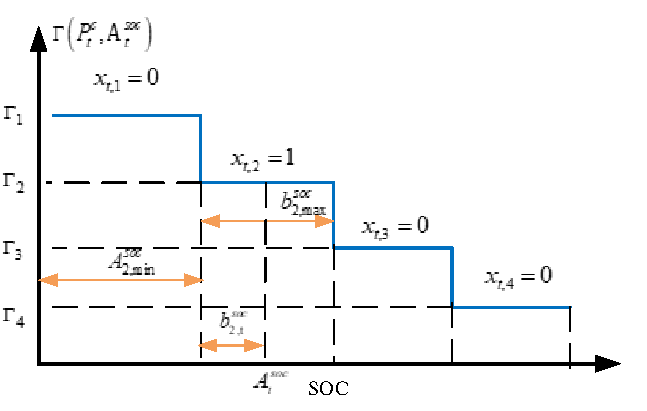
\includegraphics[scale=0.85]{figures/Chap3-3-dual-SOC-approx.pdf}
  \caption{特性曲线$\Gamma \left( {P_t^c,A_t^{soc}} \right)$的近似化处理示例}
  \label{fig:dual-SOC-approx}
\end{figure}

相应地,储气SOC可线性化为\cite{CAES-Wind-Rui-19}
\begin{subequations}
\label{equ:dual-SOC-approx-example}
\begin{gather}
%m_t^{ch} = P_t^c\sum\nolimits_j {x_{t,j}^{}} {\Gamma _j} \label{equ:non-dual-SOC-approx}\\
A_t^{soc} = \sum\limits_j {({b_{j,t}^{soc} + x_{t,j}^{}A_{j,\min }^{soc}})}, \forall t \label{equ:dual-SOC-approx-example-1} \\
0 \le b_{j,t}^{soc} \le x_{t,j}^{}b_{j,\max }^{soc},\sum\limits_j {x_{t,j}^{}}  = 1, \forall t, j \label{equ:dual-SOC-approx-example-2}
\end{gather}
\end{subequations}
其中,$b_{j,max}^{soc}$表示$A_t^{soc}$的分段$j$的长度;$A_{j,min}^{soc}$表示储气SOC分段$j$的起始值;$b_{j,t}^{soc}$为储气SOC处于分段$j$时偏离 $A_{j,min}^{soc}$的偏移量。(\ref{equ:dual-SOC-approx-example-1})给出了储气SOC的分段线性表示方法;(\ref{equ:dual-SOC-approx-example-2})限制任一分段$j$的偏移量$b_{j,t}^{soc}$不超过该分段的长度。

由于$P_t^cx_{t,j}$项的存在,约束(\ref{equ:non-dual-SOC-approx})为非线性约束,可采用大M法线性化为\cite{CAES-Wind-Rui-19}
\begin{subequations}
\label{equ:dual-SOC-approx-example-big-M}
\begin{gather}
m_t^{ch} = \sum\limits_j {z_{t,j}}, \forall t \\
P_{\min }^c{x_{t,j}} \le {z_{t,j}} \le P_{\max }^c{x_{t,j}}, \forall t, j\\
P_{\min }^c({1 - {x_{t,j}}})\le {x_{t,j}} - {z_{t,j}} \le P_{\max }^c({1 - {x_{t,j}}}), \forall t,j
\end{gather}
\end{subequations}
其中,$z_{t,j}$为辅助连续量。

AA-CAES储能电站的其它宽工况热力学特性曲线($\Psi$, $\varphi$,$\phi$)亦可采用(\ref{equ:non-dual-SOC-approx})-(\ref{equ:dual-SOC-approx-example-big-M})所示的分段线性化方法进行转化\cite{CAES-Wind-Rui-19}。从而,AA-CAES与风电协同系统调度运行模型转化为混合整数线性规划问题,可通过CPLEX等求解器进行求解。

需要说明的是,采用上述方法近似(\ref{equ:coup-heat-power})及(\ref{equ:coup-mass-SOC})中的热力学特性函数时存在引入了较多整数变量的风险
\footnote{若需减少整数变量个数,可考虑采用文献~\inlinecite{Thesis-Andrew-18}提出的整数变量较少的MILP建模方法。},对模型的求解存在一定影响。考虑到风速的日周期性及日前市场竞标规则,基于滚动优化思想,本节将模型(\ref{eq:WT-CAES-Co-Gen-Model}) 按日分为365个子问题,相邻子问题间通过储气SOC与储热SOC 建立联系,从而实现模型的高效求解\cite{CAES-Wind-Rui-19}。事实上,该类思路在含储能的电力系统运行规划问题中已被采用,如文献~\inlinecite{CXY-Plan-18}。

\subsection{标准风电场算例分析}

本节基于实际风速数据分析风-储协同系统的发电能力,重点关注AA-CAES宽工况运行特性的影响,并进行灵敏度分析,以评估储能容量与储能功率对风-储协同系统发电能力的影响\cite{CAES-Wind-Rui-19}。仿真计算由哈佛大学Odyssey超算服务器集群\footnote{https://www.rc.fas.harvard.edu/odyssey/}与Matlab并行计算工具包完成,模型采用YALMIP\cite{YALMIP}建模,求解器为Gurobi 8.0.1。

\subsubsection{系统参数}
为便于讨论,本节通过将为风电场配置的AA-CAES储能电站的容量分配到单个风机进行分析。选取中国2015年~500~个地区的全年风速数据进行仿真\footnote{风速数据源自 https://www.renewables.ninja/},假定风电场采用金风GW 77/1500系列1.5MW风机,其切入风速为3m/s,额定风速为11m/s, 切出风速为22m/s。

假定与风机协同运行的等效AA-CAES电站采用图\ref{fig:CAES-thermal-struc}所示的两级压缩与两级膨胀结构,压缩机和透平具有相同的额定功率,考虑~1.5MW(Capacity-1)和~1.0MW (Capacity-2)两种情形\cite{CAES-Wind-Rui-19}。除设计质量流率由两种额定功率界定外,其它参数与文献\inlinecite{CAES-IES-16-Rui} 相同,储气库容积为2000m$^3$(1.5MW/12h~储能),工作压力范围为8.4MPa-9MPa。 两级压缩机的设计压比分别为11.5、7.83, 设计等熵效率分别为0.85、0.81,设计入口温度分别为15$^\circ$C、40$^\circ$C。两级透平的设计膨胀比分别为8.94、9.4,设计等熵效率分别为0.82、0.82,设计入口温度均为280$^\circ$C。

%需要说明的是,储气库可采用文献[15]中的钢管储气方案,增设于风机塔筒内部或浅埋于风机附近地下。此外,通过提高储气库的工作压力上限或降低储气库的工作压力下限可降低对储气空间的需求量。

\subsubsection{宽工况影响分析}
配置容量为12h的储能时,所测试的~500~个地区在考虑与不考虑宽工况运行特性时容量因子相对降低量及不考虑宽工况时的容量因子如图\ref{fig:Part-Load-Exe-Cap}所示。由图\ref{fig:Part-Load-Exe-Cap}可知,对于风资源较贫乏地区,如额定工况下风-储系统的CF低于20\%的区域,计及宽工况后CF的减少量相对较少。其原因在于,该部分地区在实际场景中由于弃风限电等问题并不严重,所配置的储能一般也不进行压缩储能与膨胀释能过程,即实际中无需配置储能。对于风资源较丰富地区,如容量因子大于30\%的区域,AA-CAES宽工况特性对风-储协同运行性能的影响较大,部分地区发电能力下降达5\%\cite{CAES-Wind-Rui-19}。

将所分析的~500~个地区宽工况特性对CF影响的统计特性示于表\ref{tab:Part-load-Wind-CF}。可以得出,对风-储协同系统而言,AA-CAES宽工况运行特性对其发电能力存在不同程度的影响;与不考虑组件部分负载特性相比,考虑宽工况后风资源丰富地区CF降低>4\%。由此可见,宽工况特性对风资源丰富地区的风-储协同系统发电能力的影响不可忽视\cite{CAES-Wind-Rui-19}。
\begin{table}[htb]
  \centering
  \begin{minipage}[t]{0.60\linewidth} % 如果想在表格中使用脚注,minipage是个不错的办法
  \caption{宽工况特性对风-储协同系统CF的影响}
  \label{tab:Part-load-Wind-CF}
    \begin{tabularx}{\linewidth}{ccccc}
      \toprule[1.5pt]
      {\heiti CF 降低百分数} & >4\%  &  >2\% &  >1\%  &   >0.5\%  \\\midrule[1pt]
      Capacity 1 样本数 & 36 & 124 & 179 & 248 \\
      Capacity 2 样本数 & 4 & 102 & 143 & 185 \\
      \bottomrule[1.5pt]
    \end{tabularx}
  \end{minipage}
\end{table}

\begin{figure}[H] % use float package if you want it here
  \centering
  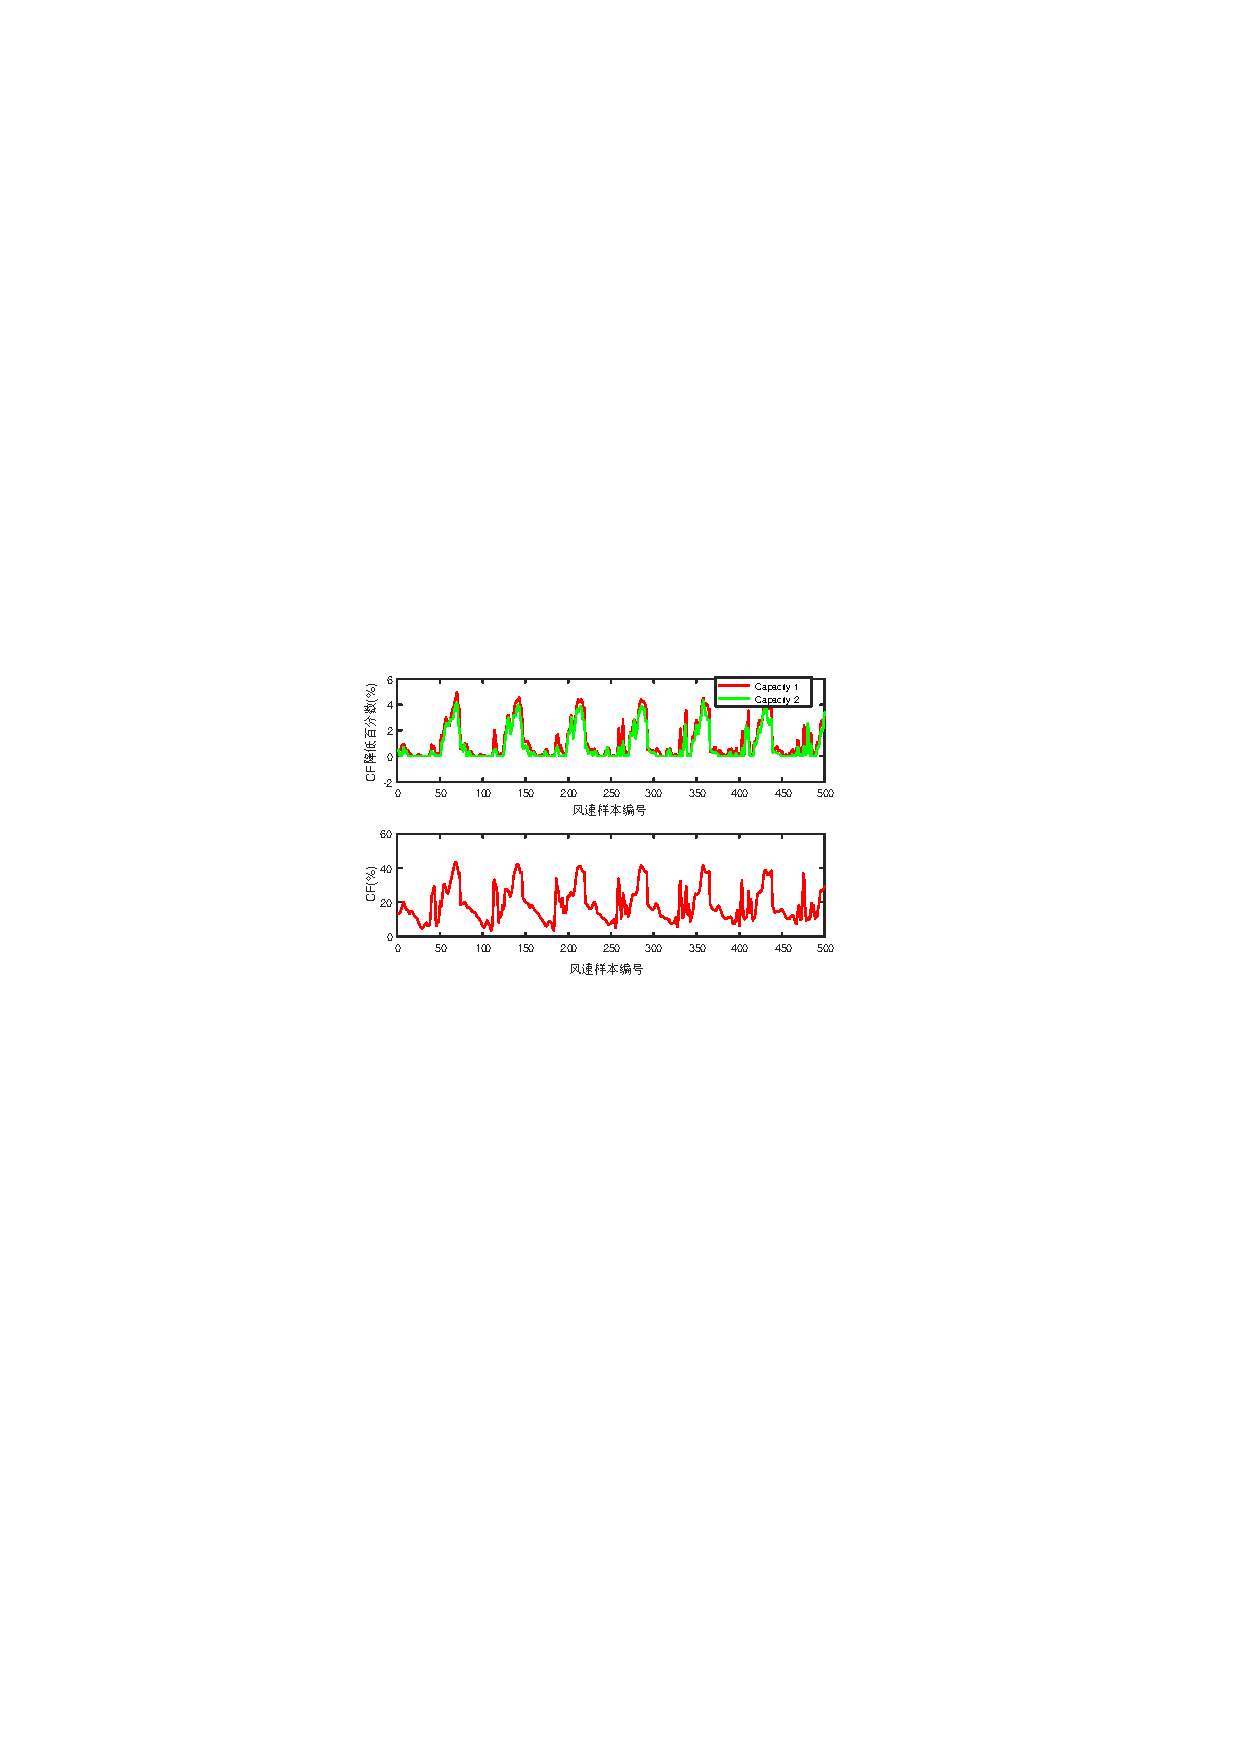
\includegraphics[scale=1.50]{figures/Chap3-15-Part-Load-Exe-Cap.pdf}
  \caption{配置12h储能时宽工况特性对协同系统CF的影响}
  \label{fig:Part-Load-Exe-Cap}
\end{figure}

\subsubsection{灵敏度分析}
对于风资源丰富地区,由于存在较为明显的弃风限电等问题(如图\ref{fig:Wind-Curtailment-Province}所给的典型省份的弃风),一般会配置一定容量的储能,以改善风电与负荷需求的时序不匹配特性。在不同的储能容量下,AA-CAES的宽工况特性对风-储协同系统的影响不同,图\ref{fig:Part-Load-Exe-Str-Sen}给出了不同储能容量时的CF折损的灵敏度分析结果。不难发现,储能容量越大,宽工况特性对风-储协同系统CF的降低(或对500个样本中CF的最大降低量)的影响将会增大,其原因在于在仿真分析中将所有储能容量下的最小储气与储热SOC与设置为最大SOC的5\%;储能容量越大,储进去相同的风电,为了保持最小SOC要求,储能容量大的需要保持较多的能量,才能维持储气罐压力,从而导致其所能释放的风电减少,增大了宽工况对风-储协同运行容量因子的影响\cite{CAES-Wind-Rui-19}。从图~\ref{fig:Part-Load-Exe-Cap}中亦可看出,配置的储能功率越大,宽工况对CF 的影响也越大。因此,在风-储协同运行场景下,根据风资源情况,实现最佳的AA-CAES容量及功率配置对减小AA-CAES宽工况特性的影响尤为重要。

\begin{figure}[H] % use float package if you want it here
  \centering
  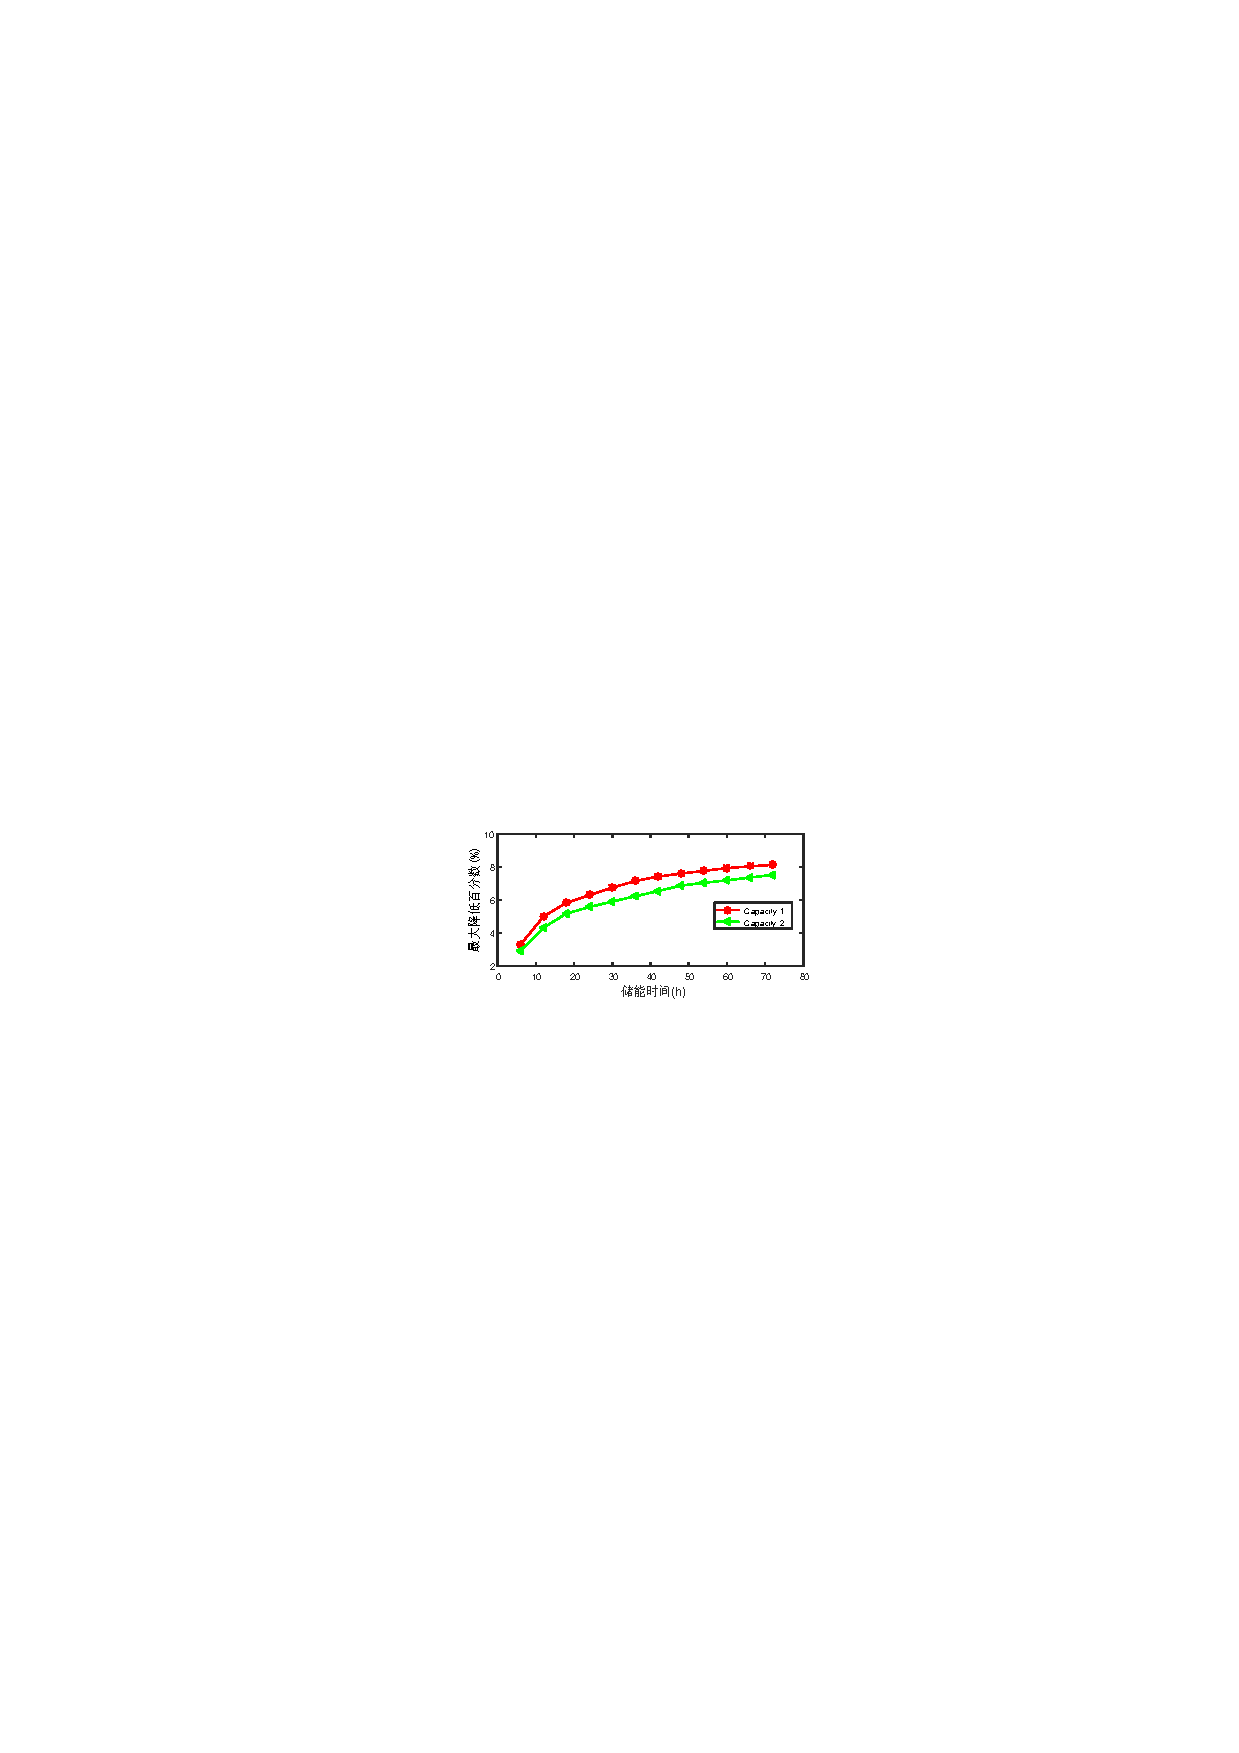
\includegraphics[scale=1.75]{figures/Chap3-15-Part-Load-Exe-Str-Sen.pdf}
  \caption{储能时间对宽工况特性影响程度的灵敏度分析}
  \label{fig:Part-Load-Exe-Str-Sen}
\end{figure}

%\section{含~AA-CAES~储能电站的电网灵活性评估}
%\label{sec:chap3-aa-caes-flex}
%\subsection{面向规划的灵活性评估}
%
%\subsection{模型转化与求解}
%
%\subsection{青海电网算例分析}
%\subsubsection{青海电网概况}
%本文第~\ref{sec:background}节指出了青海电网在可再生能源发展方面的概况。然而,映入眼帘的重要问题是青海100\%清洁能源供给模式可否持续?如何在确保可靠性的条件下实现可持续的100\%清洁能源供应系统?本节通过深入分析青海电网现状、新能源消纳现状,通过“绿电7日”与“绿电9日”模式的分析,挖掘青海电网100\%清洁能源系统不可持续的原因。进一步,基于AA-CAES 能量及备用模型分析储能电站的灵活性,并利用青海电网实际数据\footnote{本节算例中青海电网网架信息由青海电网公司提供,限于部分数据保密要求,该部分数据不予以公开。}合理评估AA-CAES储能电站对于提升可再生能源电力消纳的灵活性。
%
%\subsubsection{结果对比分析}

%\subsubsection{不计及宽工况的双SOC模型}

%\subsubsection{计及宽工况特性的双SOC模型}



%\subsubsection{{ERCOT}电网概况}


%\subsubsection{不计及宽工况的能量及备用模型}

%\subsubsection{计及宽工况的双SOC能量及备用模型}

%\subsubsection{各调度策略综合分析}

\section{面向日前电力市场的储能电站市场运营策略}
\label{sec:chap3-bid-aa-caes}
在储能产业商业化初期,有效的日前电力市场竞标策略可支撑AA–CAES储能电站的经济运行\cite{CAES-DAM-Rui-18}。储能电站参与市场运营的方式主要包括价格影响者机制与价格接受者机制,前者假定储能电站的竞标策略会影响市场电价,后者则在给定的市场价格下决定竞标电量\cite{CAES-DAM-Rui-18}。本节重点研究比较复杂的价格影响者机制下AA-CAES储能电站的竞标策略,并基于此给出价格接受者机制下的竞标策略。首先,在宽工况双SOC能量模型的基础上,提出AA–CAES储能电站的双层竞标策略;其次,在宽工况双SOC能量与备用模型的基础上,给出AA-CAES储能电站以价格接受者参与电量及备用市场的竞标策略。

\subsection{竞标模型}
\label{sec:chap3-bid-aa-caes-game}
本小节研究AA-CAES储能电站以价格影响者机制参与日前电力市场的竞标策略。在价格影响者机制下,一般可采用多层规划来刻画市场参与主体间的交互行为与决策顺序,而多层规划可用主从博弈的思想进行建模与分析\cite{Game-Mei-16}。有鉴于此,我们构建面向AA–CAES电站独立运营商的主从博弈双层竞标模型,以辅助其参与日前电力市场并实现套利运营。主从博弈竞标模型的基本思路为,AA–CAES储能电站运营商参与电力市场竞标,上报售(购)电量与售(购)电价,以最大化电力交易运营收益;电力市场交易机构根据储能电站、其它电源及负荷的竞标标的,以最大化社会福利出清电力市场。

%其次,提出AA–CAES储能电站主从博弈竞标模型的高效求解方法,其思路为通过最优性条件将该双层非线竞价模型转化为单层模型,并线性化互补松弛约束。 最后,采用布尔展开法近似线性化单层模型目标函数中的价格与电量双线性项,将单层竞价模型转化为混合整数线性规划。

\subsubsection{领导者层:储能电站}
作为市场参与主体,即主从博弈领导者(~Leader~),AA-CAES储能电站运营商以售/购电量与售/购电价为竞标标的,参与日前电力市场竞标以最大化运营收益,即
\begin{eqnarray}
\label{equ:aa-caes-pab-leader-obj}
\begin{array}{l}
\mathop {\max \;}\limits_{{\Xi _{UP}}} \sum\limits_{j = 1}^{{N_A}} {\sum\limits_{t = 1}^{{N_T}} {({\lambda _{j,t}^{dis}A_{j,t}^{dis} - \lambda _{j,t}^{ch}A_{j,t}^{ch}})} } - \sum\limits_{j = 1}^{{N_A}} {\sum\limits_{t = 1}^{{N_T}} {({C_j^{dis}A_{j,t}^{dis} + C_j^{ch}A_{j,t}^{ch}})} }
\end{array}
\end{eqnarray}
其中,$N_A$为储能电站运营商所辖的AA-CAES电站个数;$N_T$为日前电力市场总决策时段,本节取为24;$\lambda _{j,t}^{ch}$与$\lambda _{j,t}^{dis}$分别为~AA-CAES~ 储能电站向电力市场的购电报价与售电报价;$A_{j,t}^{ch}$ 与$A_{i,t}^{dis}$ 分别表示电力市场出清的储能电站购电量与充电量,对任一电站$j$,$A_{j,t}^{ch}$与$A_{i,t}^{dis}$ 分别与双SOC模型中的$P_t^c$与$P_t^d$相同\footnote{由于日前电力市场调度时段间隔一般为1h,本节在不引起混淆的情况下混用电量与容量。};$C_j^{ch}$与$C_j^{dis}$分别为电站在压缩储能及膨胀释能模式下的边际运行成本。第一项表示AA-CAES储能电站向电力市场的套利收益(扣除购电成本),第二项表示总的边际运行成本。

AA-CAES储能电站的决策变量$\Xi_{UP}$主要包括向电力市场交易机构上报的竞标标的(售购电量与售购电价),电站自身运行状态量(压缩功率与膨胀功率、储热功率与耗热功率)、储气SOC、储热SOC等\cite{CAES-DAM-Rui-18}。储能电站主的从博弈竞标策略模型中,上层目标函数的约束条件包括电站自身运行约束与下层模拟的电力市场出清约束,其自身运行约束除包括第\ref{sec:dual-SOC-energy}节提出的双SOC能量模型(\ref{equ:coup-heat-power})、(\ref{equ:coup-mass-SOC})、(\ref{equ:air-SOC-energy})及(\ref{equ:TES-SOC-energy})以及运行限制约束(\ref{eq:WT-CAES-Power-Limit})外,还包括如下的竞标标的限制约束:
\begin{subequations}
\label{equ:aa-caes-pab-bid-cons}
\begin{gather}
0 \le \hat A_{j,t}^{ch} \le u_{j,t}^{ch}\bar A_j^{ch},\;0 \le \hat A_{j,t}^{dis} \le u_{j,t}^{dis}\bar A_j^{dis}, \forall j,t \label{equ:aa-caes-PAB-quantity} \\
\lambda _{j}^{ch,l} \le \lambda _{j,t}^{ch} \le \lambda _{j}^{ch,u},\sum\nolimits_{t = 1}^{{N_T}} {\lambda _{j,t}^{ch}}  \le {N_T}\lambda _{j,av}^{ch} \label{equ:aa-caes-PAB-price-ch},\forall j,t \\
\lambda _{j}^{dis,l} \le \lambda _{j,t}^{dis} \le \lambda _{j}^{dis,u},\sum\nolimits_{t = 1}^{{N_T}} {\lambda _{j,t}^{dis}} \le {N_T}\lambda _{j,av}^{dis} \label{equ:aa-caes-PAB-price-dis}, \forall j,t
\end{gather}
\end{subequations}
其中,$\hat A_{j,t}^{ch}$与$\hat A_{j,t}^{dis}$分别为储能电站售购电量竞标标的;$\bar A_j^{ch}$与$\bar A_j^{dis}$为电站的压缩机容量与膨胀机容量,对于任一电站$j$,其值分别与$P_{max}^c$与$P_{max}^d$相同;$\lambda_j^{ch,l}$(或$\lambda_j^{dis,l}$)与$\lambda_j^{ch,u}$(或$\lambda_j^{dis,u}$)分别为购电电价(或售电电价)的最小值与最大值。(\ref{equ:aa-caes-PAB-quantity})要求向电力市场上报的售购电量竞标标的不能超过其额定压缩与膨胀容量;(\ref{equ:aa-caes-PAB-price-ch})与(\ref{equ:aa-caes-PAB-price-dis})分别限制AA-CAES储能电站的购电电价与售电电价在一定范围内,同时要求平均售/购电价不能超过设定值$\lambda _{j,av}^{dis}$ 与 $\lambda _{j,av}^{ch}$,该值由AA-CAES电站运营商与电力市场签订的合同决定。

\subsubsection{跟随者层:市场出清}
作为AA-CAES储能电站运营商主从博弈竞标策略的跟随者(Follower),电力市场交易机构根据~AA-CAES~储能电站、其它电源及负荷竞标标的,以最大化电力市场社会福利为目标出清电力市场\cite{CAES-DAM-Rui-18},从而向市场参与主体提供购(售)电量与购(售)电价信号\footnote{此处假定电力市场出清采用以报价结算方式。},即
\begin{eqnarray}
\label{equ:aa-caes-pab-follow-obj}
\begin{array}{l}
\mathop {\min \;}\limits_{{\Xi _{LL}}\;} \sum\limits_{t = 1}^{{N_T}} {\sum\limits_{j = 1}^{{N_A}} {\left[ {\lambda _{j,t}^{dis}A_{j,t}^{dis} - \lambda _{j,t}^{ch}A_{j,t}^{ch}} \right]} } + \sum\limits_{t = 1}^{{N_T}} {\sum\limits_{i = 1}^{{N_G}} {C_{i,t}^gp_{i,t}^g} }  - \sum\limits_{t = 1}^{{N_T}} {\sum\limits_{i = 1}^{{N_D}} {C_{i,t}^dp_{i,t}^d} }
\end{array}
\end{eqnarray}
其中,$C_i^g$ 为常规机组报价;$p_{i,t}^g$为常规机组出清电量;$p_{i,t}^d$ 为负荷出清量;$C_{i,d}$为负荷报价;$N_G$为常规机组个数;$N_D$为负荷个数。目标函数中第一项对应AA-CAES储能电站;第二项与第三项分别对应常规机组与电力负荷。

电力市场出清决策变量${\Xi_{LL}}$主要包括各电源与负荷的中标量、市场出清电价及电网状态变量(线路传输功率、电压等),而约束条件主要包括各电源与负荷运行约束及输电网潮流约束组成\cite{CAES-DAM-Rui-18}。本节采用直流潮流模型描述输电网潮流分布\cite{MATPOWER},具体地:
\begin{subequations}
\label{equ:DC-flow}
\begin{gather}
p_{i,t}^g + W_{i,t}^{} + A_{i,t}^{dis} = A_{i,t}^{ch} + p_{i,t}^d + \sum\limits_{l|F(l) = i} {P_t^l}  - \sum\limits_{l|T(l) = i} {P_t^l} ,\forall i,\forall t \label{equ:DC-flow-bus-power}\\
P_t^l = ({{\theta _{F(l),t}} - {\theta _{T(l),t}}})/{X_l},\forall l,\forall t \label{equ:DC-flow-line-power}\\
0 \le A_{j,t}^{ch} \le \hat A_{j,t}^{ch}, 0 \le A_{j,t}^{dis} \le \hat A_{j,t}^{dis},\;\forall j,\forall t \label{equ:aa-caes-pab-quan-upper}\\
\left\{\begin{aligned}
&0 \le p_{i,t}^g \le p_i^{g,u},0 \le W_{i,t}^{} \le W_{i,t}^u, p_{i,t}^{d,l} \le p_{i,t}^d \le p_{i,t}^{d,u},\;\forall i,\forall t\\
& - P_l^u \le P_t^l \le P_l^u,\forall l,\forall t\\
&  - \pi  \le {\theta _{i,t}} \le \pi ,{\theta _{ref,t}} = 0,\;\forall i,\forall t
\end{aligned}\right.\label{equ:aa-caes-pab-others}
\end{gather}
\end{subequations}
其中,$W_{i,t}$为节点$i$注入的风电功率;$P_t^l$为线路$l$传输的功率;$F(l)$与$T(l)$分别代表线路$l$的首节点与末节点;$\theta _{f(l),t}$ 与$\theta _{t(l),t}$ 表示线路首末节点电压相角;$X_l$为线路阻抗。(\ref{equ:DC-flow-bus-power})描述节点功率平衡关系;(\ref{equ:DC-flow-line-power})描述线路潮流分布;(\ref{equ:aa-caes-pab-quan-upper}) 表征市场出清的AA-CAES储能电站售/购电量(或功率)不超过电站运营商上报的售/购电量(或功率);(\ref{equ:aa-caes-pab-others}) 给定常规机组出力、风电机组出力、线路潮流及节点电压相角的上下限。事实上,由于本节只涉及日前电量市场,因此假定负荷需求全部由日前市场满足,即$ p_{i,t}^{d,l}= p_{i,t}^d = p_{i,t}^{d,u}$,如此目标函数(\ref{equ:aa-caes-pab-follow-obj})中可去除最后一项。

综上,在价格影响者机制下(多个储能电站协同或大容量储能电站情形),AA-CAES电站运营商的主从博弈竞标模型为
\begin{subequations}
\label{equ:bid-model-price-marker}
\begin{gather}
\mathop {\max \;}\limits_{{\Xi _{UP}}} \sum\limits_{j = 1}^{{N_A}} {\sum\limits_{t = 1}^{{N_T}} {({\lambda _{j,t}^{dis}A_{j,t}^{dis} - \lambda _{j,t}^{ch}A_{j,t}^{ch}})} } - \sum\limits_{j = 1}^{{N_A}} {\sum\limits_{t = 1}^{{N_T}} {({C_j^{dis}A_{j,t}^{dis} + C_j^{ch}A_{j,t}^{ch}})}}\label{equ:bid-model-price-marker-obj}\\
\mbox{s.t.}~
\mbox{AA-CAES双SOC能量模型}\\
\mbox{AA-CAES运行限制约束}\\
\mbox{竞标标的限制约束}\\
\mbox{电力市场出清问题} 
\end{gather}
\end{subequations}

\subsection{竞标模型的典型扩展形式}
\label{sec:chap3-self-schedu}

在第\ref{sec:chap3-bid-aa-caes-game}节中,我们给出了在价格影响者机制下,基于双SOC能量模型的AA-CAES储能电站市场竞标模型。该模型可进一步推广至储能电站容量较小时的价格接受者机制,同时也扩展至计及备用容量及备用调用等情形。本小节重点给出主从博弈竞标模型的几类推广形式,为了表述简洁,此处仅关注单个AA-CAES储能电站,为此相关变量退化采用\ref{sec:dual-SOC}节中的符号。特别地,我们将基于双SOC能量与备用模型给出储能电站以价格接受者同时参与电量及备用市场的竞标模型,以供相应的电力市场运营问题使用。首先,给出不考虑价格不确定性的确定性竞标策略;其次,建立采用盒式不确定集刻画价格不确定性的~AA-CAES~鲁棒竞标策略;最后,给出计及备用调用的随机竞标策略。

\textbf{(1)确定性竞标策略}

当不考虑价格不确定性,采用价格接受者机制时储能电站宽工况竞标模型的目标函数为
\begin{equation}
\label{equ:aa-caes-self-schedule-DT}
\mathop {\max }\limits_{\Xi_{DT}}  \underbrace {\sum\limits_{t = 1}^{N_T} {\left[ {\lambda_t^E({P_t^d - P_t^c})\Delta t + \lambda_t^{sr}({P_t^{c,sr} - P_t^{d,sr}}) + \lambda_t^{nr}P_t^{d,nr}} \right]} \; - \sum\limits_{t = 1}^{N_T} {({C^{dis}P_t^d + C^{ch}P_t^c})} }_{DT}
\end{equation}
其中,$\lambda_t^E$,$\lambda_t^{sr}$及$\lambda_t^{nr}$分别为日前电量及备用市场中的电量价格、旋转备用与非旋转备用价格。第\ref{sec:chap3-bid-aa-caes-game} 节中我们用$\lambda_t^{dis}$与$\lambda_t^{ch}$区分了价格影响者机制下的膨胀释能与压缩储能过程的竞标电价,此处由于采用了价格接受者机制,用(预测的)市场电价$\lambda_t^E$代替二者。确定性竞标策略的约束集$\Xi_{DT}$由双SOC能量及备用模型(\ref{equ:coup-heat-power})、(\ref{equ:coup-mass-SOC})、(\ref{equ:def-Pc-Pd-eq})、(\ref{equ:air-SOC-reserve})、(\ref{equ:TES-SOC-reserve})、(\ref{equ:coup-mass-heat-SOC-reserve})
以及运行限制约束(\ref{eq:WT-CAES-Power-Limit})界定。

\textbf{(2)鲁棒竞标策略}

若考虑电量价格、旋转备用价格及非旋转备用价格的不确性,可采用不确定性集合来描述电价,进而可构建鲁棒竞标策略。描述不确定性的方式主要有盒式不确定集(无穷范数)、椭球不确定集(欧式范数)以及多面体不确定集(1范数)等\cite{Robust-Self-Schedule-Review-18}。此处仅给出基于盒式不确定集合的竞标策略,若采用其它不确定集描述价格不确定性时,该鲁棒竞标策略亦可相应推广。

盒式不确定集通过无穷范数来约束随机变量,即电量价格、旋转备用及非旋转备用价格可描述为
\begin{equation}
\label{equ:price-uncertainty-BS}
B{S^\Upsilon } = \left\{ {\tilde \lambda _t^\Upsilon  \in \left[ {\Lambda _t^\Upsilon  - \hat \Lambda _t^\Upsilon ,\;\Lambda _t^\Upsilon  + \hat \Lambda _t^\Upsilon } \right],\left| {\frac{{\tilde \lambda _t^\Upsilon  - \Lambda _t^\Upsilon }}{{\hat \Lambda _t^\Upsilon }}} \right| \le \Psi _B^\Upsilon ,\forall t} \right\},\Upsilon  = \left\{ {E,sr,nr} \right\}
\end{equation}
其中,$\Psi _B^\Upsilon  \in \left[ {0,1} \right],\Upsilon  = \left\{ {E,sr,nr} \right\}$。

基于盒式不确定集的鲁棒竞标目标函数为
\begin{equation}
\mathop {\max }\limits_\Xi  \mathop {\min }\limits_{\tilde \lambda _t^\Upsilon  \in B{S^\Upsilon }} \left\{ {\sum\limits_{t = 1}^{N_T} {\left[ {\tilde \lambda _t^E({P_t^d - P_t^c}) + \tilde \lambda _t^{sr}({P_t^{c,sr} - P_t^{d,sr}}) + \tilde \lambda _t^{nr}P_t^{d,nr}} \right]} \; - \sum\limits_{t = 1}^{N_T} {({C^{dis}P_t^d + C^{ch}P_t^c})}} \right\}
\end{equation}
从而,基于盒式不确定集的~AA-CAES~鲁棒竞标策略为
\begin{equation}
\label{equ:aa-caes-self-schedule-BS-uncertainty}
\arg \;\mathop {\max }\limits_\Xi  \left\{ {DT - \Psi _B^E\sum\limits_{t = 1}^{N_T} {\tilde \lambda _t^E({P_t^d - P_t^c})} -\Psi _B^{sr}\sum\limits_{t = 1}^{N_T} {\tilde \lambda _t^{sr}({P_t^{c,sr} - P_t^{d,sr}})} - \Psi _B^{nr}\sum\limits_{t = 1}^{N_T} {\tilde \lambda _t^{nr}P_t^{d,nr}} } \right\}
\end{equation}

%不同于盒式不确定集,椭球不确定集采用欧式范数刻画不确定集\cite{Robust-Self-Schedule-Review-18},即
%\begin{equation}
%\label{equ:price-uncertainty-ES}
%E{S^\Upsilon } = \left\{ {\tilde \pi _t^\Upsilon  \in \left[ {\Pi _t^\Upsilon  - \hat \Pi _t^\Upsilon ,\;\Pi _t^\Upsilon  + \hat \Pi _t^\Upsilon } \right],\sqrt {{{\sum\nolimits_{t = 1}^T {\left( {\frac{{\tilde \pi _t^\Upsilon  - \Pi _t^\Upsilon }}{{\hat \Pi _t^\Upsilon }}} \right)} }^2}}  \le \Psi _E^\Upsilon ,\forall t} \right\},\Upsilon  = \left\{ {E,sr,nr} \right\}
%\end{equation}
%其中,$\Psi _B^\Upsilon  \in \left[ {0,\sqrt {\left| T \right|} } \right],\Upsilon  = \left\{ {E,sr,nr} \right\}$.

%相应地,基于椭球不确定集的~AA-CAES~鲁棒自调度策略为:
%\begin{equation}
%\label{equ:aa-caes-self-schedule-ES-uncertainty}
%\begin{array}{l}
%\arg \;\mathop {\max }\limits_\Omega  \left\{ {DT - \Psi _B^E\sqrt {\sum\limits_{t = 1}^T {{{\left( {\tilde \pi _t^E} \right)}^2}{{\left( {P_t^d - P_t^c} \right)}^2}} }  - \Psi _B^{sr}\sqrt {\sum\limits_{t = 1}^T {{{\left( {\tilde \pi _t^{sr}} \right)}^2}{{\left( {P_t^{c,sr} - P_t^{d,sr}} \right)}^2}} } } \right.\\
%\;\;\;\;\;\;\;\;\;\;\;\;\;\left. { - \Psi _B^{nr}\sqrt {\sum\limits_{t = 1}^T {{{\left( {\tilde \pi _t^{nr}} \right)}^2}{{\left( {P_t^{d,nr}} \right)}^2}} } } \right\}
%\end{array}
%\end{equation}

%(3) 多面体不确定集

%不同于盒式与椭球不确定集,多面体不确定及采用1范数描述不确定集合\cite{Robust-Self-Schedule-Review-18},即电价的鲁棒不确定集为
%\begin{equation}
%\label{equ:price-uncertainty-PS}
%P{S^\Upsilon } = \left\{ {\tilde \pi _t^\Upsilon  \in \left[ {\Pi _t^\Upsilon  - \hat \Pi _t^\Upsilon ,\;\Pi _t^\Upsilon  + \hat \Pi _t^\Upsilon } \right],\sum\nolimits_{t = 1}^T {\left| {\frac{{\tilde \pi _t^\Upsilon  - \Pi _t^\Upsilon }}{{\hat \Pi _t^\Upsilon }}} \right|}  \le \Psi _P^\Upsilon ,\forall t} \right\},\Upsilon  = \left\{ {E,sr,nr} \right\}
%\end{equation}

%由此,基于多面体不确定集的AA-CAES鲁棒自调度策略为:
%\begin{equation}
%\label{equ:aa-caes-self-schedule-PS-uncertainty}
%\begin{array}{l}
%\arg \;\mathop {\max }\limits_\Omega  \left\{ {DT - \Psi _B^E{v^E} - \Psi _B^{sr}{v^{sr}} - \Psi _B^{nr}{v^{nr}}} \right\}\\
%\;\;\;\;\;s.t.\;{v^E} \ge \tilde \pi _t^E\left( {P_t^d - P_t^c} \right),{v^E} \ge 0,\forall t\\
%\;\;\;\;\;\;\;\;\;\;{v^{sr}} \ge \tilde \pi _t^{sr}\left( {P_t^{c,sr} - P_t^{d,sr}} \right),\;{v^{sr}} \ge 0,\forall t\\
%\;\;\;\;\;\;\;\;\;\;{v^{nr}} \ge \tilde \pi _t^{nr}P_t^{d,nr}{v^{nr}} \ge 0,\forall t\;
%\end{array}
%\end{equation}

\textbf{(3)计及备用调用的随机竞标策略}

AA-CAES确定性竞标策略(\ref{equ:aa-caes-self-schedule-DT})及鲁棒竞标策略(\ref{equ:aa-caes-self-schedule-BS-uncertainty})并未考虑实时电力市场中的备用调用,若计及AA-CAES备用容量的调用,即采用双SOC能量及备用扩展模型时,AA-CAES储能电站的宽工况随机竞标模型目标函数为
\begin{equation}
\label{equ:aa-caes-self-schedule-ST}
\begin{array}{l}
\mathop {\max }\limits_{\Xi_{S}} \sum\limits_{s = 1}^{{N_S}} {{r_s}} \left\{ {\underbrace {\sum\limits_{t = 1}^{N_T} {[ {\lambda _{t,s}^E({P_t^d - P_t^c}) + \lambda _{t,s}^{sr}({P_t^{c,sr} - P_t^{d,sr}}) + \lambda _{t,s}^{nr}P_t^{d,nr}}]} }_{D_{st}^{{R_1}}}} \right.\;\\
\;\;\;\;\;\;\;\; + \underbrace {\sum\limits_{t = 1}^{N_T} {\lambda _{t,s}^E[{({P_t^{d,sr} + P_t^{c,sr}})u_{t,s}^{sr} + P_t^{d,nr}u_{t,s}^{nr}}]} }_{D_{st}^{{R_2}}}\\
\;\;\;\;\;\;\; - \left. {\;\underbrace {\sum\limits_{t = 1}^{N_T} {[{C^{dis}({\overbrace {P_t^d + P_t^{d,sr}u_{t,s}^{sr} + P_t^{d,nr}u_{t,s}^{nr}}^{P_t^{d,Ev}}}) + C^{ch}({\overbrace {P_t^c - P_t^{c,sr}u_{t,s}^{sr}}^{P_t^{c,Ev}}})}]} }_{D_{st}^{{R_3}}}} \right\}
\end{array}
\end{equation}
其中,$r_s$为场景$s$下电力市场电价$\lambda_t^E$,$\lambda_t^{sr}$及$\lambda_t^{nr}$的概率。约束集$\Xi_{S}$由双SOC能量及备用扩展模型(\ref{equ:def-power-relation})、(\ref{equ:air-SOC-reserve-exten})、(\ref{equ:TES-SOC-reserve-exten})、(\ref{equ:coup-heat-power-reserve-exten})以及运行限制约束(\ref{eq:WT-CAES-Power-Limit})共同界定。事实上,模型(\ref{equ:aa-caes-self-schedule-ST})可进一步计及条件风险价值,但不在本章讨论范围之内。

%本文第~\ref{cha:ca-recs} 章会针对风速不确定性讨论基于条件风险价值的新型风-储(压缩空气储能)系统日前电力及备用市场竞标策略。

%\subsection{{ERCOT}算例分析}
%本小节以美国{ERCOT}电网为例,分析AA-CAES储能电站宽工况运行特性对其在电量及备用市场自调度策略的影响,从而明晰在备用特性分析中计及宽工况运行特性的必要性与重要性。此处选择{ERCOT}电网进行分析主要原因在于:1)ERCOT电网电价、负荷及机组参数等公开信息较全面\footnote{国内访问ERCOT电网数据受限,本部分的基础数据由苏黎世联邦理工学院 Jared Garrison 博士提供。};2)ERCOT电网具有很高的风电装机渗透率;3)ERCOT电网具有电量及备用市场;4)ERCOT电网目前规划了D-CAES电站的建设,其规划容量达300MW。需要说明的是,考虑ERCOT电力市场的一种退化情形,即假定电价 具有固定的峰谷价差,即可在一定程度上表征中国电力市场。

\subsection{模型求解策略}
AA-CAES的市场竞标模型及典型各种扩展形式中,以价格影响者机制的主从博弈竞标模型为双层模型,直接求解困难,而其典型扩展形式均为单层模型,比较容易求解。有鉴于此,本小节重点给出双层竞标模型的求解方法,并在下一小节中进行算例分析。

~AA-CAES~电站主从博弈双层竞标模型(\ref{equ:bid-model-price-marker})为非线性模型,下层电力市场出清为线性规划,可利用最优性条件(KKT条件)将该双层模型转化为单层规划\cite{CAES-DAM-Rui-18}。转化后的单层模型亦为非线性,除AA-CAES热力学特性曲线簇引入的非线性外,其非线性来源主要包括两类,一是通过最优性条件引入的互补松弛约束,二是上层目标函数中价格与能量双线性乘积项\cite{CAES-DAM-Rui-18}。为此,本节采用布尔展开法近似双线性乘积项\cite{Binary-Expansion-1},最终将主从博弈双层竞价模型转化为混合整数线性规划。

\subsubsection{最优性条件}
下层电力市场出清为线性规划, 可采用最优性条件消去其目标函数。 为便于描述,将下层电力市场出清问题(\ref{equ:aa-caes-pab-follow-obj})(\ref{equ:DC-flow})抽象为
\begin{eqnarray}
\begin{array}{l}
\min \;{f^T}x\\
s.t.\;\;{A_{eq}}x = {b_{eq}}:\;\lambda \\
\;\;\;\;\;\;{A_{ineq}}x \le {b_{ineq}}:\mu
\end{array}
\end{eqnarray}
其对应的等价~KKT~系统为
\begin{subequations}
\label{eq:EKKT}
\begin{gather}
{A_{eq}}x = {b_{eq}}, {A_{ineq}}x \le {b_{ineq}}, f = A_{eq}^T\lambda  - A_{ineq}^T\mu, \\
 0 \le {\mu} \bot ({ - {A_{ineq}}x + {b_{ineq}}}) \ge 0 \label{eq:KKT-non}
\end{gather}
\end{subequations}

最优性条件(\ref{eq:EKKT})中引入了非线性互补松弛约束(\ref{eq:KKT-non}),其抽象形式为
\begin{eqnarray}
\label{eq:add}
0 \le \left( {a - f} \right) \bot g \ge 0
\end{eqnarray}
为便于求解,将(\ref{eq:add})线性化为
\begin{eqnarray}
\label{equ:aa-caes-big-M}
0 \le a - f \le Mh,\;0\le g \le M\left( {1 - h} \right)
\end{eqnarray}
其中,$h$为引入的布尔量;$M$ 为一足够大的正数。

\subsubsection{布尔展开法}
上层目标函数(\ref{equ:aa-caes-pab-leader-obj})中存在电价与电量相乘的双线性项,如$\lambda _{j,t}^{dis}A_{j,t}^{dis}$与$\lambda _{j,t}^{ch}A_{j,t}^{ch}$。 针对该类双线性项,采用布尔展开法\cite{Binary-Expansion-1,Binary-Expansion-2}近似线性化。以线性化$\lambda _{j,t}^{dis}A_{j,t}^{dis}$为例,可将$\lambda _{j,t}^{dis}$展开为
\begin{eqnarray}
\label{equ:aa-caes-ben-1}
\lambda _{j,t}^{dis} = \lambda _j^{dis,l} + \Delta \lambda _j^{dis}\sum\limits_{k = 0}^{{K_1}} {{2^k}} x_{j,t,k}^{dis},\forall j,\forall t
\end{eqnarray}
并附加如下约束:
\begin{subequations}
\label{equ:aa-caes-ben-append}
\begin{gather}
0 \le A_{j,t}^{dis} - z_{j,t,k}^{dis} \le M({1 - x_{j,t,k}^{dis}}),\forall j,\forall t,\forall k\\
0 \le z_{j,t,k}^{dis} \le Mx_{j,t,k}^{dis},\forall j,\forall t,\forall k\\
\Delta \lambda _j^{dis} = ({\lambda _j^{dis,u} - \lambda _j^{dis,l}})/G,\;G = {2^{{K_1}}},\forall j
\end{gather}
\end{subequations}
其中,$x_{j,t,k}^{dis}$为引入的辅助布尔变量;$z_{j,t,k}^{dis}$为辅助连续量;$\Delta \lambda _j^{dis}$为售电电价的离散步进量。$\lambda _{j,t}^{ch}A_{j,t}^{ch}$ 亦可采用相同的方式线性化。

布尔展开式(\ref{equ:aa-caes-ben-append})的近似精确度可通过离散点个数进行控制,引入的布尔量与离散点数的复杂度为[$O(\log_2{K})$],其中~$K$~为近似段数。例如,对于区间[0,1]的连续量采用32个离散点近似时,只需5个布尔量即可。此外,AA-CAES双SOC模型中的特性曲线的近似处理可采用第\ref{sec:wind-ESS-operation-model-appro}中的转化方法。

经过上述变换,面向日前电力市场的~AA-CAES~储能电站主从博弈竞标模型的MILP近似模型的目标函数为
\begin{eqnarray}
\begin{array}{l}
\mathop {\max \;}\limits_{\Xi_{UP-MILP}} \sum\limits_{t = 1}^{{N_T}} {\sum\limits_{j = 1}^{{N_A}} {[{\lambda _j^{dis,l}A_{j,t}^{dis} + \Delta \lambda _j^{dis}\sum\limits_{k = 0}^{{K_1}} {{2^k}} z_{j,t,k}^{dis}}]} } \\
\;\;\;\;\;\;\;\;\; - \sum\limits_{t = 1}^{{N_T}} {\sum\limits_{j = 1}^{{N_A}} {[{\lambda _j^{ch,l}A_{j,t}^{ch} + \Delta \lambda _j^{ch}\sum\limits_{k = 0}^{{K_2}} {{2^k}} z_{j,t,k}^{ch}}]} } \\
\;\;\;\;\;\;\;\;\; - \sum\limits_{j = 1}^{{N_A}} {\sum\limits_{t = 1}^{{N_T}} {[{C_j^{dis}A_{j,t}^{dis} - C_j^{ch}A_{j,t}^{ch}}]} }
\end{array}
\end{eqnarray}
其中,可行域$\Xi_{UP-MILP}$由以下约束限定:宽工况双SOC运行约束及其近似化方法,电站电量及电价竞标标的约束(\ref{equ:aa-caes-pab-bid-cons}),电力市场出清条件~KKT~系统中的等式约束(\ref{eq:EKKT}),采用大~M~法线性化非线性互补约束~(\ref{eq:KKT-non})~ 后得到的线性约束(\ref{equ:aa-caes-big-M}),线性化目标函数引入的约束(\ref{equ:aa-caes-ben-1})-(\ref{equ:aa-caes-ben-append}),以及采用(\ref{equ:dual-SOC-approx-example}) 与(\ref{equ:dual-SOC-approx-example-big-M})的方法近似的热力学特性曲线簇。

\subsection{IEEE系统算例分析}
本小节采用改进的~IEEE-24~节点可靠性测试系统分析AA-CAES储能电站的主从博弈竞标策略。该测试系统拓扑可参见文献\inlinecite{CAES-DAM-Rui-18},主要包含10台发电机组、32条输电线路、6座风电场、1座AA-CAES电站。AA-CAES电站布置于母线\#19,风电场位于母线 \#3,\#5,\#7,\#16,\#21,\#23。AA-CAES电站采用两级压缩、两级膨胀结构,采用定压-滑压运行方式,具体参数如表\ref{tab:AA-CAES-para}所示,其它机组参数、线路参数可参考文献\inlinecite{IEEE-RTS-24-2016}。%~AA-CAES~ 电站内部热力学特性曲线采用第~\ref{sec:chap2-bound-measure}节仿真参数。

\begin{table}[htb]
  \centering
  \begin{minipage}[t]{0.65\linewidth} % 如果想在表格中使用脚注,minipage是个不错的办法
  \caption{AA-CAES储能电站参数}
  \label{tab:AA-CAES-para}
    \begin{tabularx}{\linewidth}{ccccc}
      \toprule[1.5pt]
    参数 & $\bar A^{\rm ch}$,$\bar A^{\rm dis}$ & $\lambda^{\rm ch}$,$\lambda^{\rm dis}$ & $pr$ & $\lambda_{\rm av}^{\rm ch}$,$\lambda_{\rm av}^{\rm dis}$ \\\midrule[1pt]
  单位 & MW & $\$$/MWh & MPa & $\$/$MWh \\
  数值 & 150,350 & [35.55,69.47] & [8.4,9.0]&  47.47 \\
      \bottomrule[1.5pt]
    \end{tabularx}
  \end{minipage}
\end{table}

%\subsubsection{等效电池模型结果}
%\subsubsection{双SOC模型结果}
%\subsubsection{讨论与分析}

系统中各电源在各时段的报价最大值、最小值及平均值如图\ref{fig:AA-CAES-PAB-Price}所示,假定AA-CAES储能电站压缩储能电价与膨胀释能电价在各电源报价的最大与最小值之间。同时,储能电站24 时段平均报价不能超过各电源边际电价确定的平均值。

\begin{figure}[H] % use float package if you want it here
  \centering
  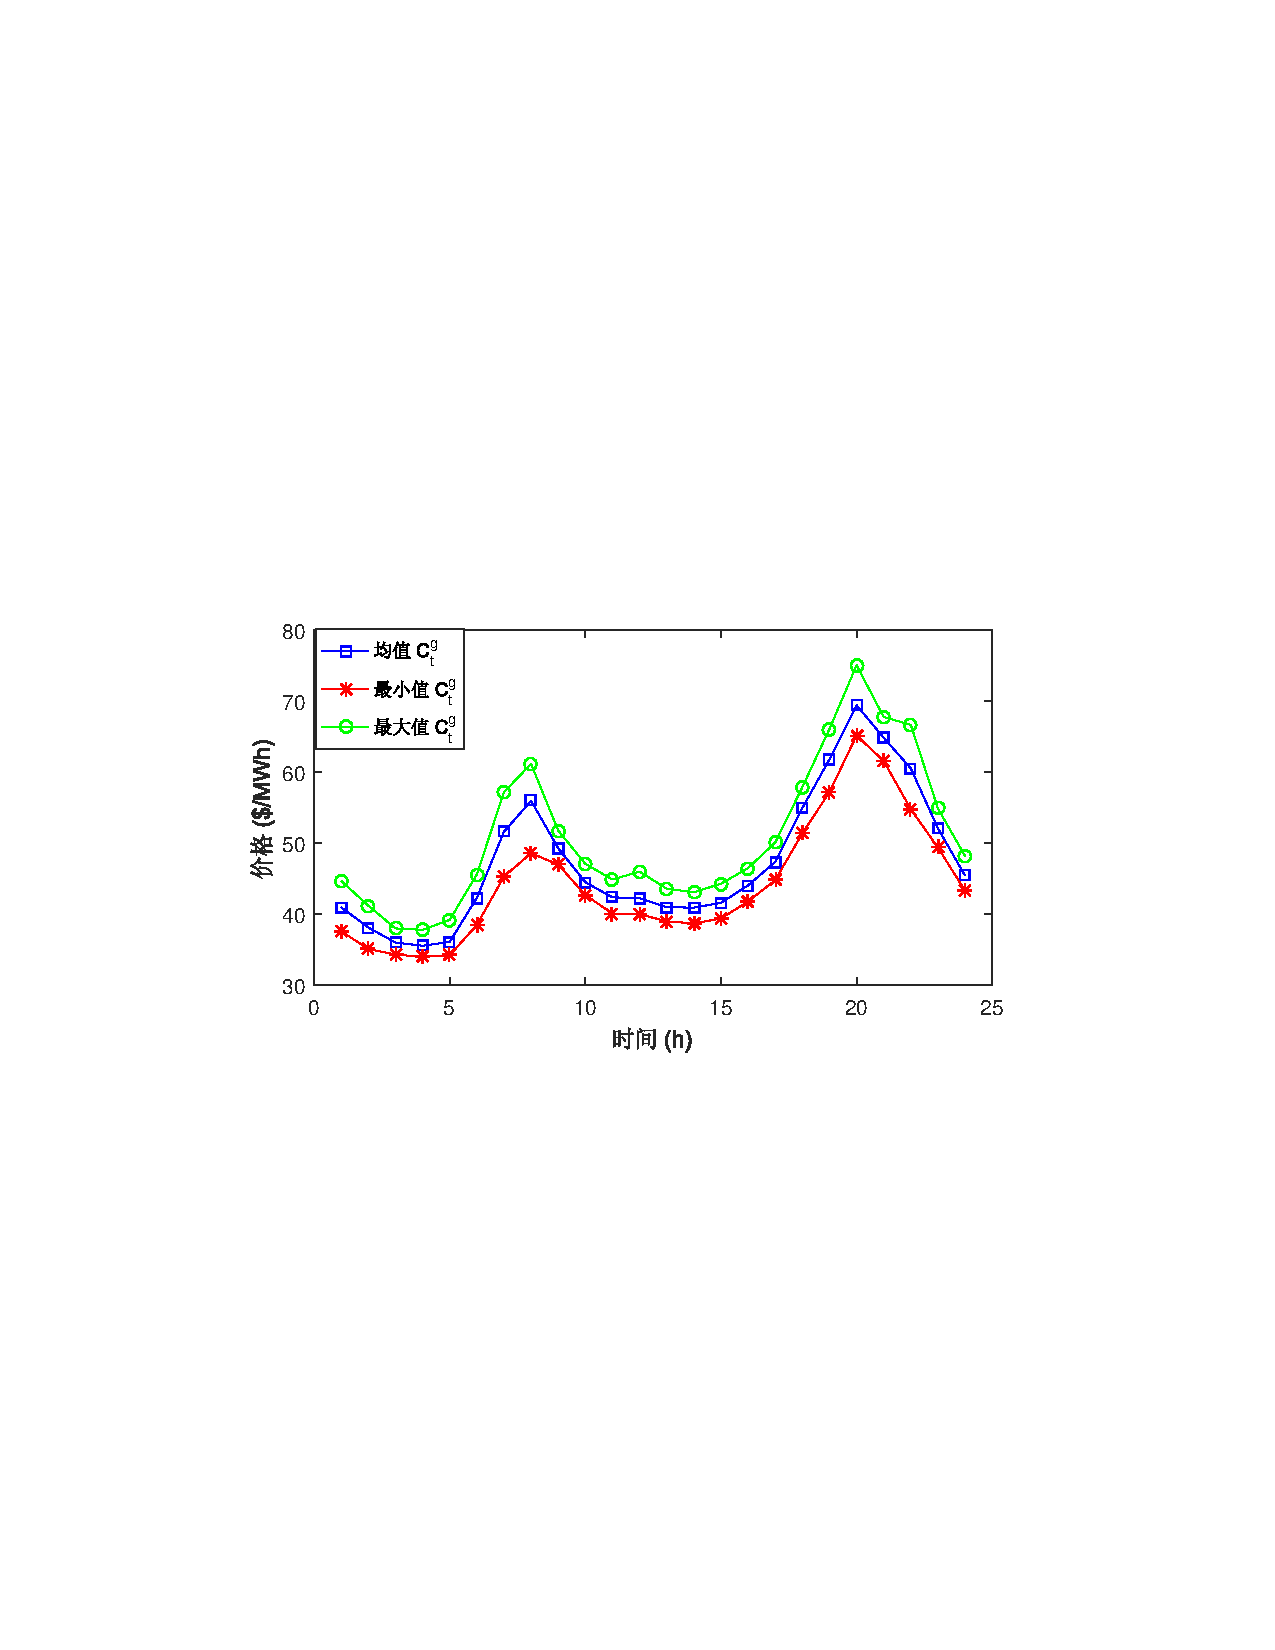
\includegraphics[scale=0.72]{figures/Chap3-10-PAB-Price.pdf}
  \caption{常规机组边际电价}
  \label{fig:AA-CAES-PAB-Price}
\end{figure}

图\ref{fig:Part-Load-PAB-Bid}给出了AA--CAES日前电力市场主从博弈竞标策略,包含购/售电价标的与购/售电量标的,图~\ref{fig:AA-CAES-PAB-LoadGen}给出了系统各电源出力水平。 AA-CAES储能电站在时段6至时段9时压缩储能,并在系统负荷高峰期其它电源难以满足系统总负荷需求时以高价释能售电,如时段11、12、15、16、19、20 等。

\begin{figure}[H] % use float package if you want it here
  \centering
  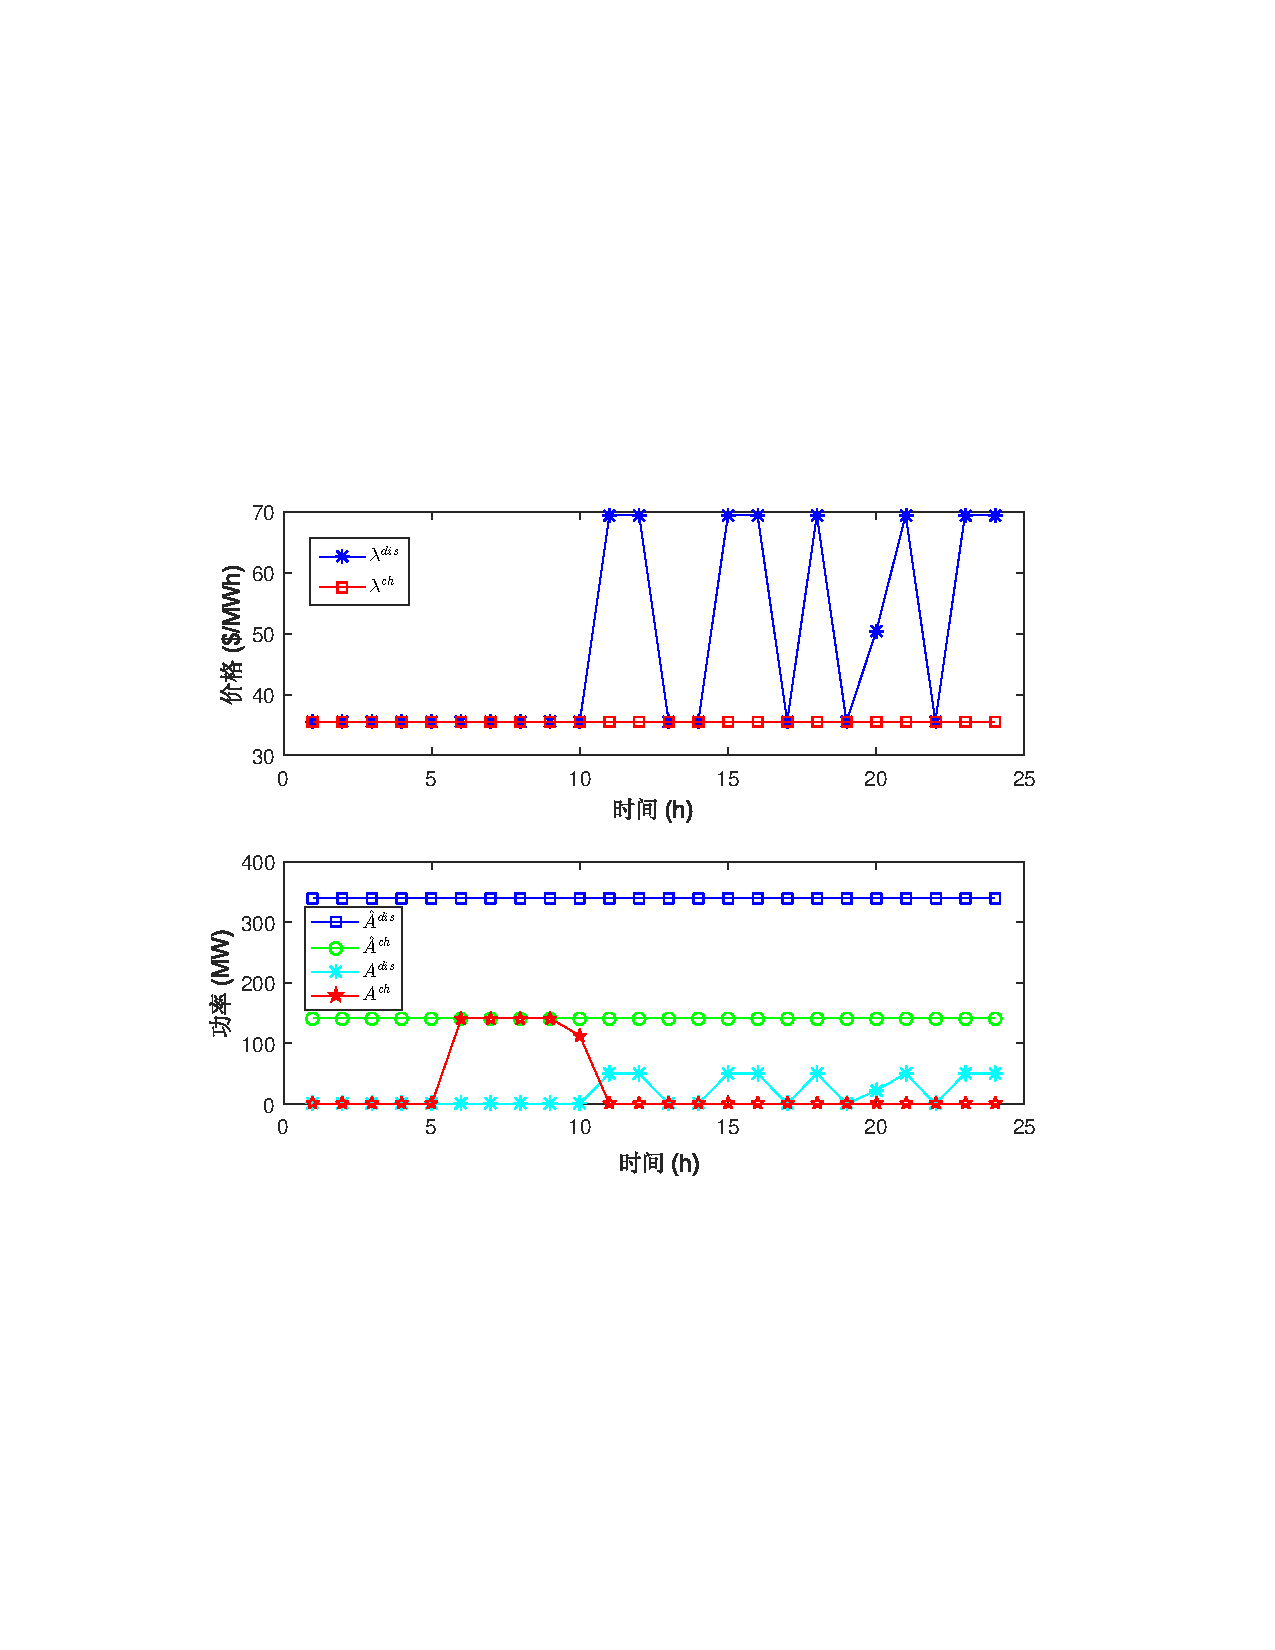
\includegraphics[scale=0.70]{figures/Chap3-10-PAB-Bid.pdf}
  \caption{AA-CAES储能电站竞标策略}
  \label{fig:Part-Load-PAB-Bid}
\end{figure}

由图\ref{fig:AA-CAES-PAB-Price}与图\ref{fig:Part-Load-PAB-Bid} 可知,AA-CAES电站以低价购入电量,再以高价售出电量,从而实现套利运营,在当前策略下日前套利运营的收益为\$19548。 特别地, 由于本节市场机制采用按报价支付的方式结算,AA-CAES~电站运营商以最高价 \$69.47 作为售出电价报价,以最低价\$35.55 作为购入电价报价,同时为满足报价平均值限制,部分时刻如时段20以低于最高价的价格报价。

\begin{figure}[H] % use float package if you want it here
  \centering
  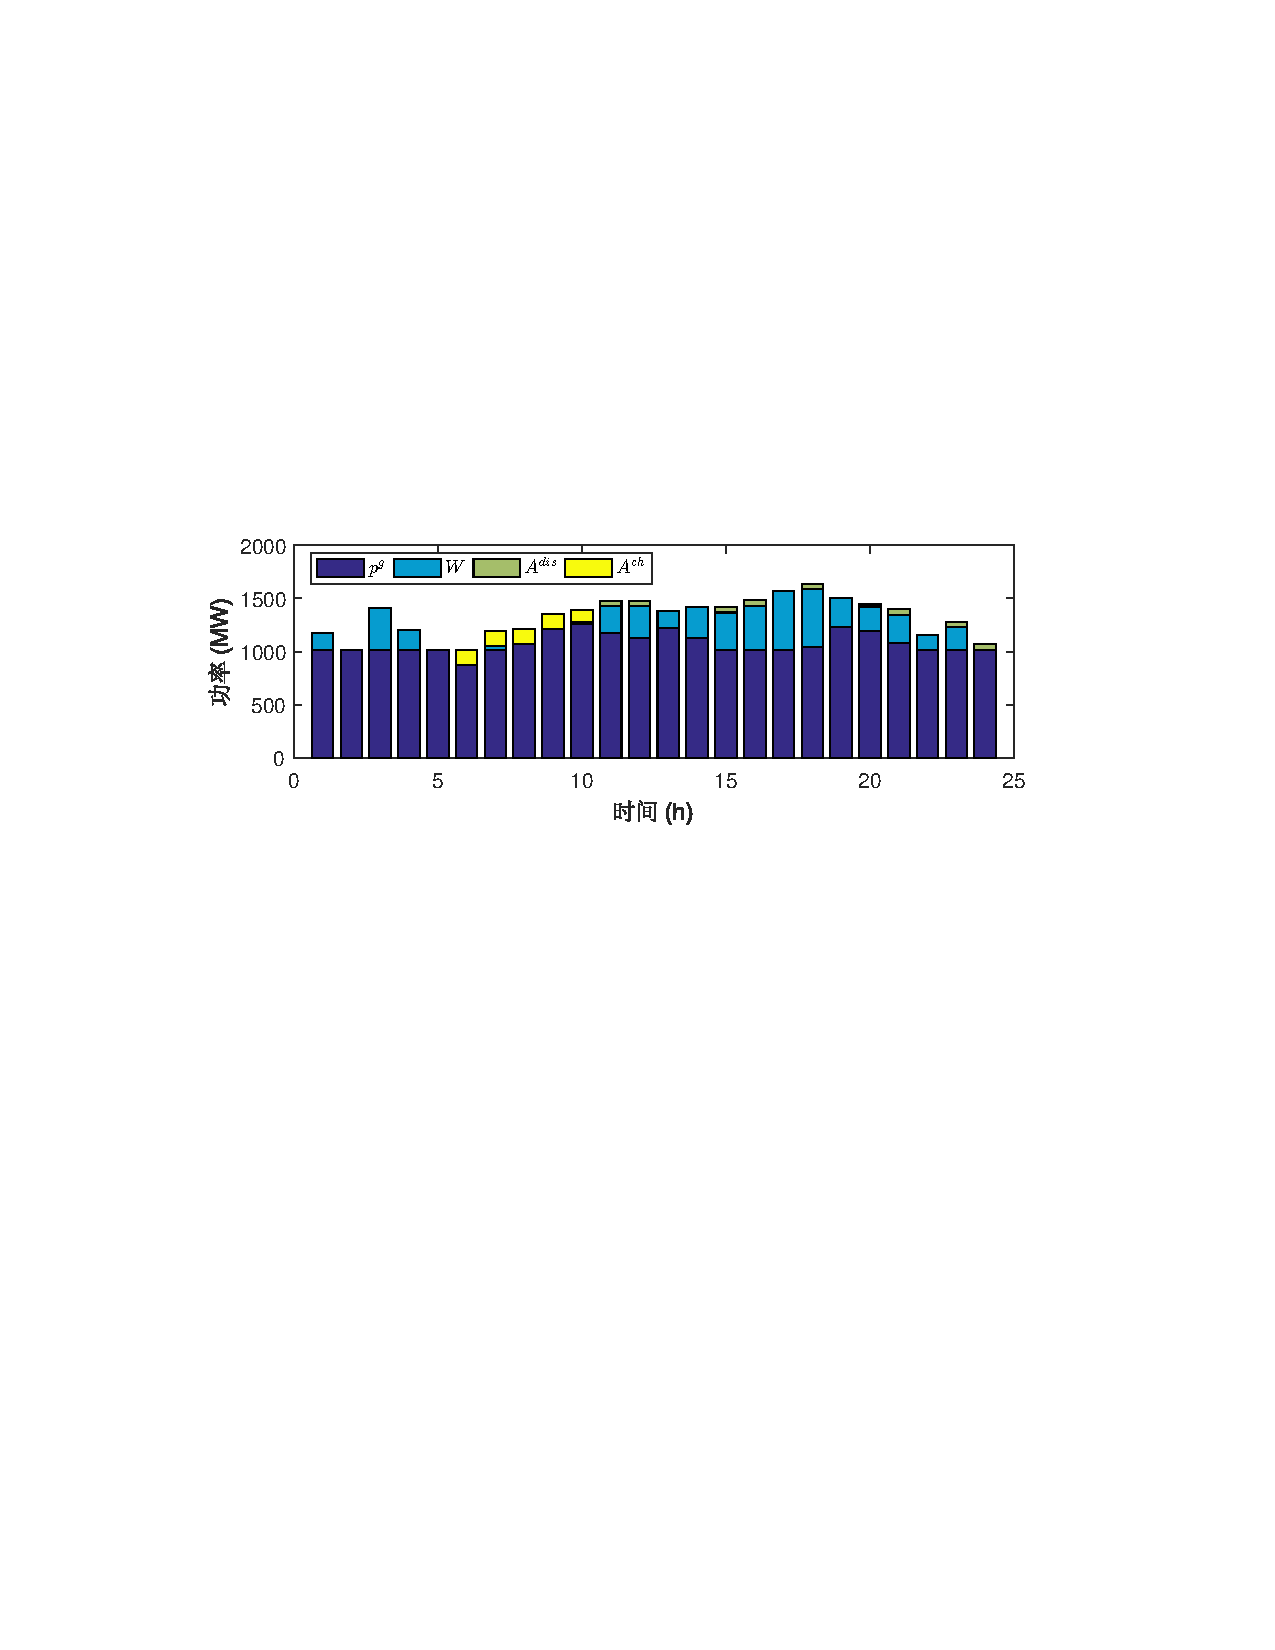
\includegraphics[scale=0.75]{figures/Chap3-10-PAB-LoadGen.pdf}
  \caption{系统各电源出力水平}
  \label{fig:AA-CAES-PAB-LoadGen}
\end{figure}

\begin{figure}[H] % use float package if you want it here
  \centering
  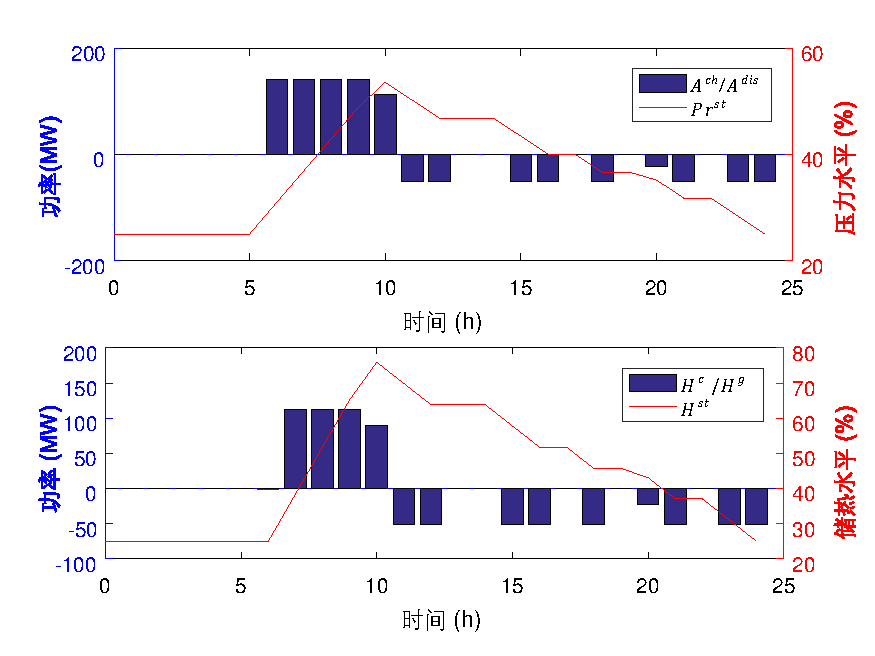
\includegraphics[scale=0.75]{figures/Chap3-10-PAB-SOC.pdf}
  \caption{AA-CAES储气水平和储热水平变化情况}
  \label{fig:Part-Load-PAB-SOC}
\end{figure}

图~\ref{fig:Part-Load-PAB-SOC}~给出了~AA-CAES~储能电站内部储气罐压力变化情况与储热水平变化情况。系统初始储热水平及储气库储气水平(百分比)均为25\%,AA-CAES压缩储能过程中储气水平增加,收集压缩热能提升储热水平。~AA-CAES~电站膨胀释能过程中储气室储气水平下降,由于透平发电环节需要回馈压缩热能,从而使得储热水平下降。储热系统中富余的压缩热能可供集中供暖,从而有望进一步提升~AA-CAES~电站运行收益,第4章将对此进行深入分析。图中亦可得知,压缩储能阶段几乎以额定工况运行,部分负载特性的影响不显著,膨胀释能常以部分负载工况运行,存在潜在备用收益,备用收益与部分负载导致的低效运行之间的平衡尚需进一步研究。

\section{小结}
AA-CAES技术方案最为直接的应用形式为储能电站,然而不同于常规电池储能等,AA-CAES储能电站内部具有独特的压力势能与压缩热能的解耦存储与耦合释能特性。同时,在电力系统外界宽工况运行要求下,AA-CAES储能电站的内部组件具有明显的部分负载特性。本章借鉴电池储能建模中的SOC方法,提出了基于热力学特性曲线簇的AA-CAES宽工况双SOC能量模型,能量与备用模型及扩展形式,进一步研究了计及宽工况特性的AA-CAES储能电站调度策略及日前电力市场竞标策略,为以储能电站形式应用于电力系统的AA-CAES的建模、运行及运营等问题提供了初步的建模方法。

\chapter{荷侧先进绝热压缩空气能量枢纽建模及运行方法}
\label{cha:st-caes}

\section{概述}
\label{sec:intro}
能量枢纽具备(燃)气、热、电等多能流载体间的传递、转换及存储功能,是综合能源系统灵活性的重要体现。随着电气化供暖技术的普遍采用,区域配电网与区域供热管网将通过具备热电联供与热电联储能力的能量枢纽紧密耦合,从而实现电能(易输不易储)与热能(易储不易输)的互补,促进可再生能源电力的热电多能流协同消纳。第~\ref{cha:simulation}章提及蓄热系统通过空气压缩热能的收集、存储与回馈,使得~AA-CAES~具备了热电联产与热电联储的能力,成为潜在的热电能量枢纽
\cite{EH-Concept-07, EH-FREEDM-11},本章将从负荷侧以能量枢纽的视角挖掘AA-CAES的供能灵活性。

%第~\ref{cha:intro}章指出从源-网-荷三侧挖掘~AA-CAES~提供的常规灵活性、供能灵活性及接口灵活性,第~\ref{cha:aa-caes}章从网侧实现了基于~AA-CAES~技术的储能电站解决方案。

采用AA-CAES构建热电能量枢纽一般有两种思路,第一种思路为改造或扩展AA-CAES内部的热力循环或回热系统,使其具备更灵活的热电联供与热电联储能力,进而构建用于分布式多能联供场景的小型能量枢纽,该能量枢纽与所接入的配电网络及供热管网一般由园区级或社区级能源集成商集中运营;第二种思路是将AA-CAES视为大型能量枢纽(或集成站)内部的清洁电能存储部件,充分发挥其具有的大容量、长循环寿命等优点,以与集成站内部的热电联产机组、(电)热泵等部件实现全寿命周期的匹配,该类能量枢纽一般由独立于热网及电网的第三方主体运营管理\footnote{从AA-CAES内部储热组件的视角而言,第一种思路需要的储热单元容量较大,而第二种思路只需设计与供电相匹配的储热组件容量即可。}。本章将针对这两类AA-CAES型热电能量枢纽展开研究,分析其内部供能特性及对外热电联供特性的相互制约关系,并分析集中运营与独立运营两种环境下AA-CAES 型能量枢纽的调度运行及市场运营等问题,以充分发挥AA-CAES在热电联供场景下的供能灵活性。

本章结构安排如图\ref{fig:Hub-Flow-Chart}所示,第\ref{sec:struc-EH-CAES}节设计两类典型的AA-CAES型热电联供能量枢纽,并建立AA-CAES型能量枢纽的热电联供与热电联储模型;第\ref{sec:st-caes-dispatch}节研究含AA-CAES型能量枢纽的热电综合能源系统的调度问题,以充分发挥多能联供型能量枢纽的供能灵活性;第
\ref{sec:exergy-IES-model}节建立基于㶲理论的热电综合能源系统质量-数量联合模型,实现热电不同品位能流的差异化建模;第\ref{sec:bid-st-caes}节研究面向热电综合能源市场的能量枢纽市场竞标策略,挖掘AA-CAES型能量枢纽的热电综合能源市场交叉套利,以提升能量枢纽的运行经济性。

\begin{figure}[H] % use float package if you want it here
  \centering
  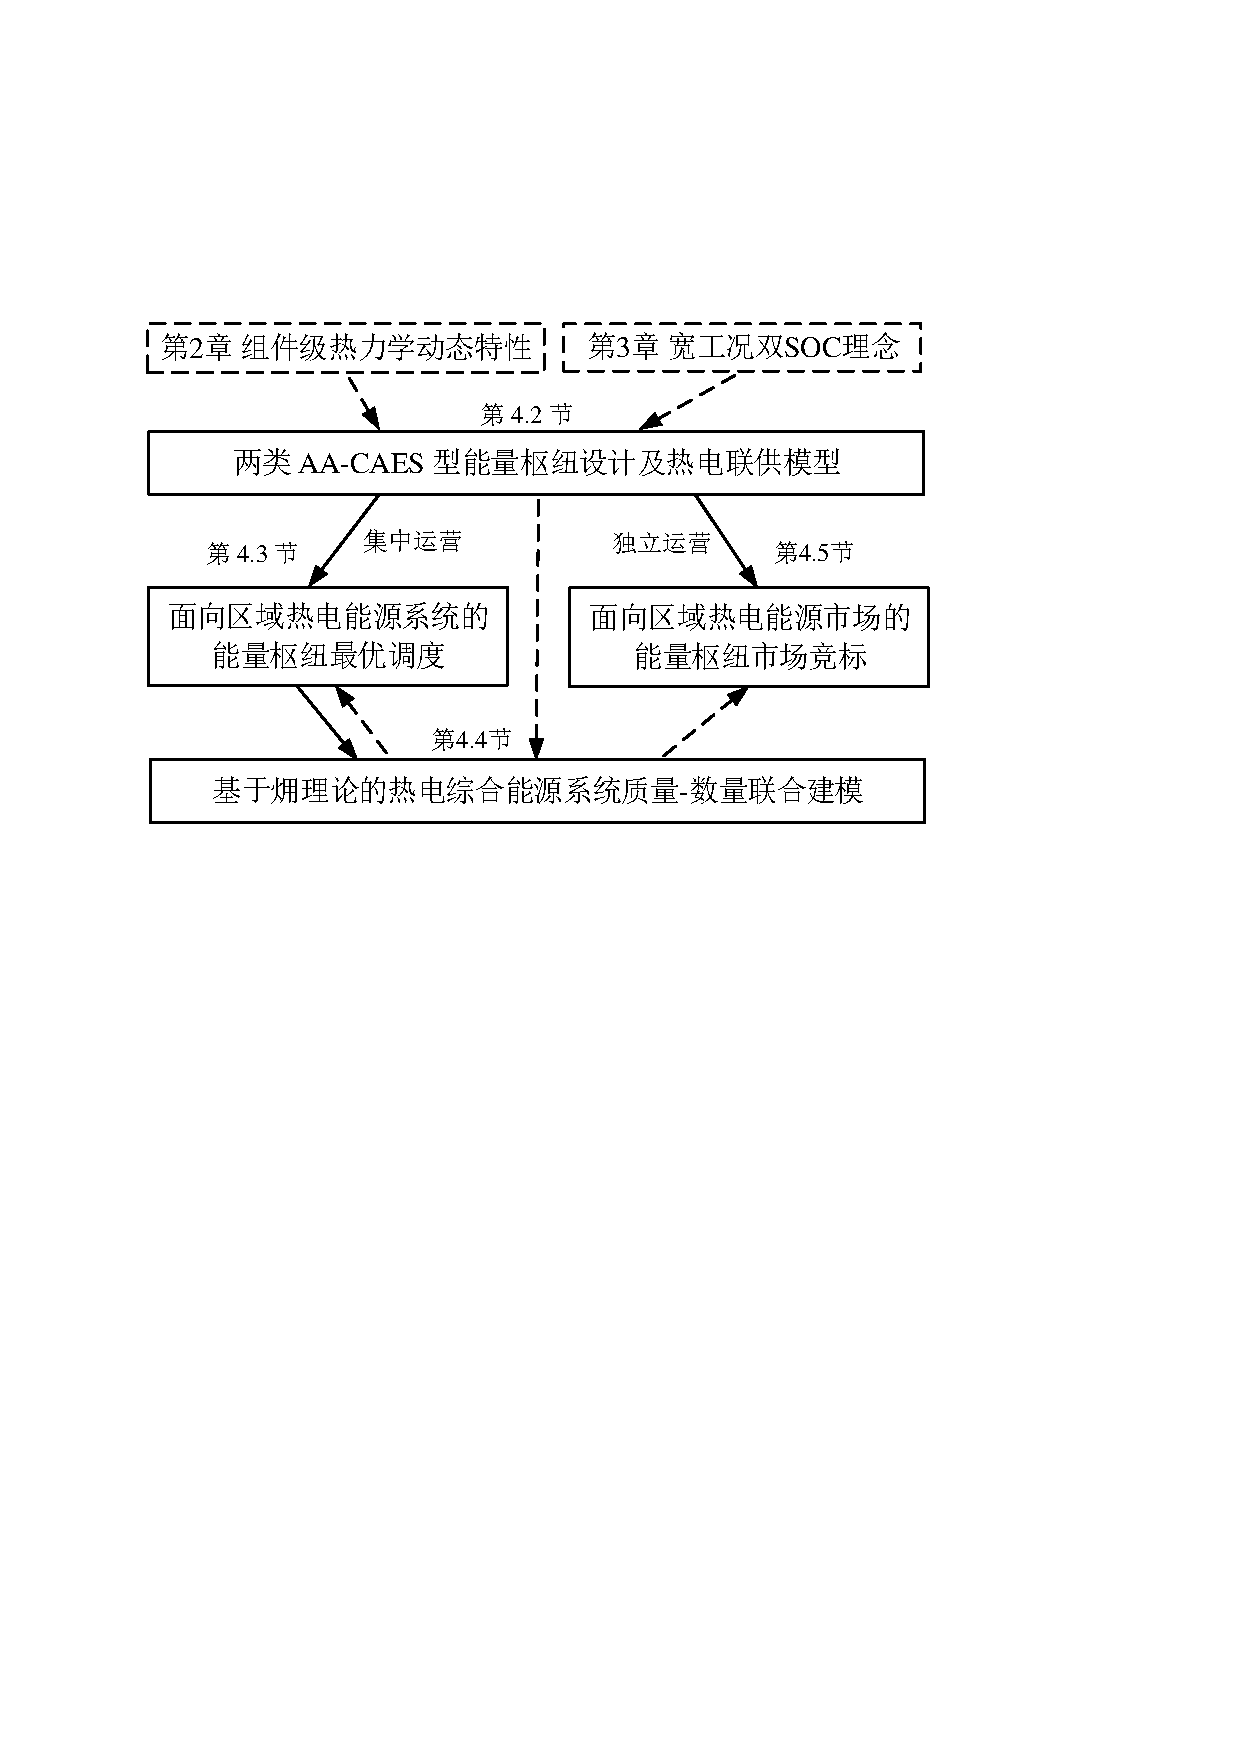
\includegraphics[scale=0.85]{figures/Chap4-1-Hub-Flow-Chart-V3.pdf}
  \caption{第4章组织结构安排}
  \label{fig:Hub-Flow-Chart}
\end{figure}

\section{先进绝热压缩空气储能能量枢纽设计及建模}
\label{sec:struc-EH-CAES}
目前已存在多种具有灵活工作模式的热电联供型AA-CAES或CAES系统,如CAES与燃气轮机构成的混合循环系统\cite{CAES-Concepts-Review-10}、AA-CAES与槽式集热构成的混合系统\cite{ST-CAES-CXT-18,ST-CAES-17}、风-光-CAES互补系统\cite{Thermo-WSCAES-17}、电阻丝与AA-CAES 配合构成的高温混合CAES系统\cite{Hybrid-CAES-14, HTH-CAES-Berk-18}、CAES 与制冷循环耦合系统\cite{CAES-Refri-06}、CAES与内燃机循环耦合系统\cite{CAES-Inner-Comb-06} 等等。本节基于该类混合型AA-CAES系统抽象出两类典型的AA-CAES型热电能量枢纽,一类为无碳排的AA-CAES型能量枢纽,另一类为大型AA-CAES能量枢纽(或集成站)。%同时建立两类能量枢纽的热电联供运行模型。

\subsection{AA-CAES型能量枢纽设计}

\textbf{(1)~I~型AA-CAES能量枢纽}

针对中国等天然气资源受限地区,可以充分利用富余的新能源电力及AA-CAES的热电联供特性设计高效灵活的I型AA-CAES能量枢纽,如图~\ref{fig:AA-CAES-Hub-V1}~所示。I 型 AA-CAES能量枢纽在经典AA-CAES结构的基础上引入了CCHP系统中普遍采用的(电)热泵(Heat Pump,HP)为能流枢纽提供额外的热量供应,从而实现灵活的热电联供与热电联储。

I型AA-CAES对外可以供电与供热(制冷),其中制冷由透平排气提供(本文忽略制冷特性),对外供热热源一方面可取自电热泵,另一方面可取自压缩热收集系统。一般而言,热电能量枢纽需具备热能与电能的缓冲能力,I型能量枢纽的电能及热能缓冲功能均由内置的AA-CAES系统实现,即由储热罐实现热能缓冲,储气罐与储热罐共同提供电能缓冲作用。I型能量枢纽挖掘了AA-CAES固有的热电联供能力,主要用于分布式多能联供场景,由园区级配电网络及供热网运营商集中运营。

\begin{figure}[H] % use float package if you want it here
  \centering
  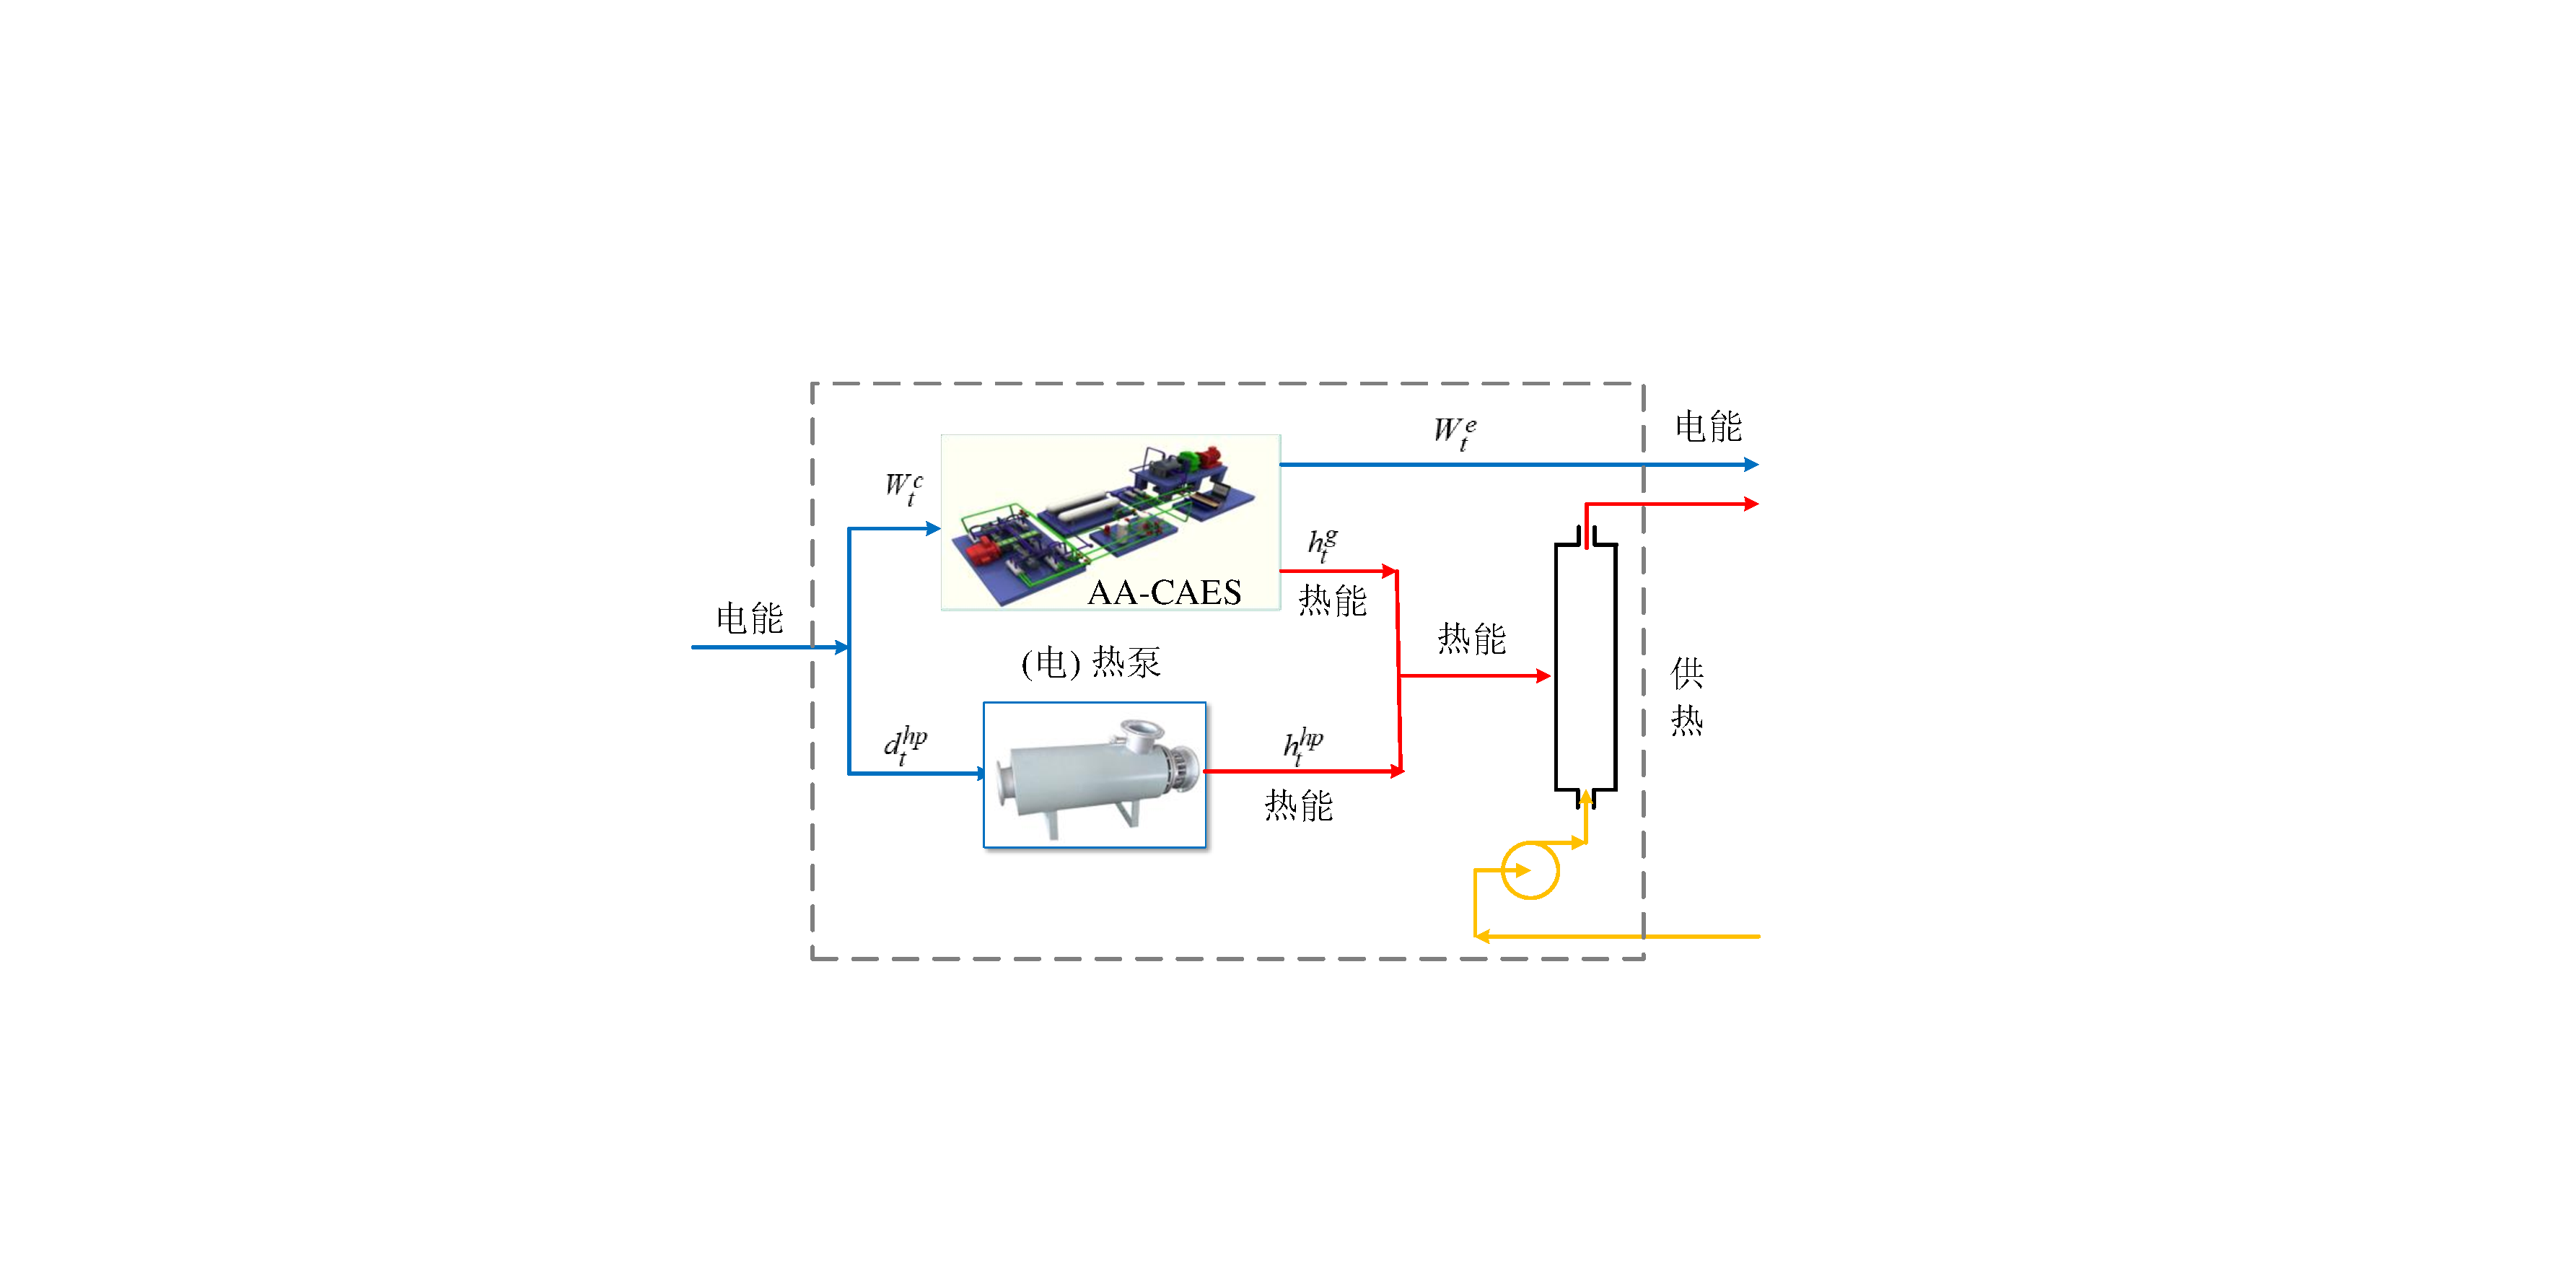
\includegraphics[scale=0.41]{figures/Chap4-2-AA-CAES-Hub-V1-3.pdf}
  \caption{~I~型AA-CAES能量枢纽结构}
  \label{fig:AA-CAES-Hub-V1}
\end{figure}

\textbf{(2)~II~型AA-CAES能量枢纽}

针对美国等页岩气开发技术成熟且具有明显经济优势的天然气资源丰富地区,可设计如图
~\ref{fig:AA-CAES-Hub-V2}~所示的II型AA-CAES能量枢纽\footnote{2016年,燃气机组超过火电等成为美国主力电源机组,而且将在相当长的一段时间内具有明显的成本优势,因此采用天然气作为II型AA-CAES能量枢纽的输入能源之一具有可行性,可参考https://energy.gov/downloads/download-staff-report-secretaryelectricity-markets-and-reliability}。其中,内置的AA-CAES 充当电能存储单元,由燃气驱动的CHP及由电能驱动的HP 为能量枢纽提供热能,而内置的TES则为能量枢纽提供热能的缓冲功能。

\begin{figure}[H] % use float package if you want it here
  \centering
  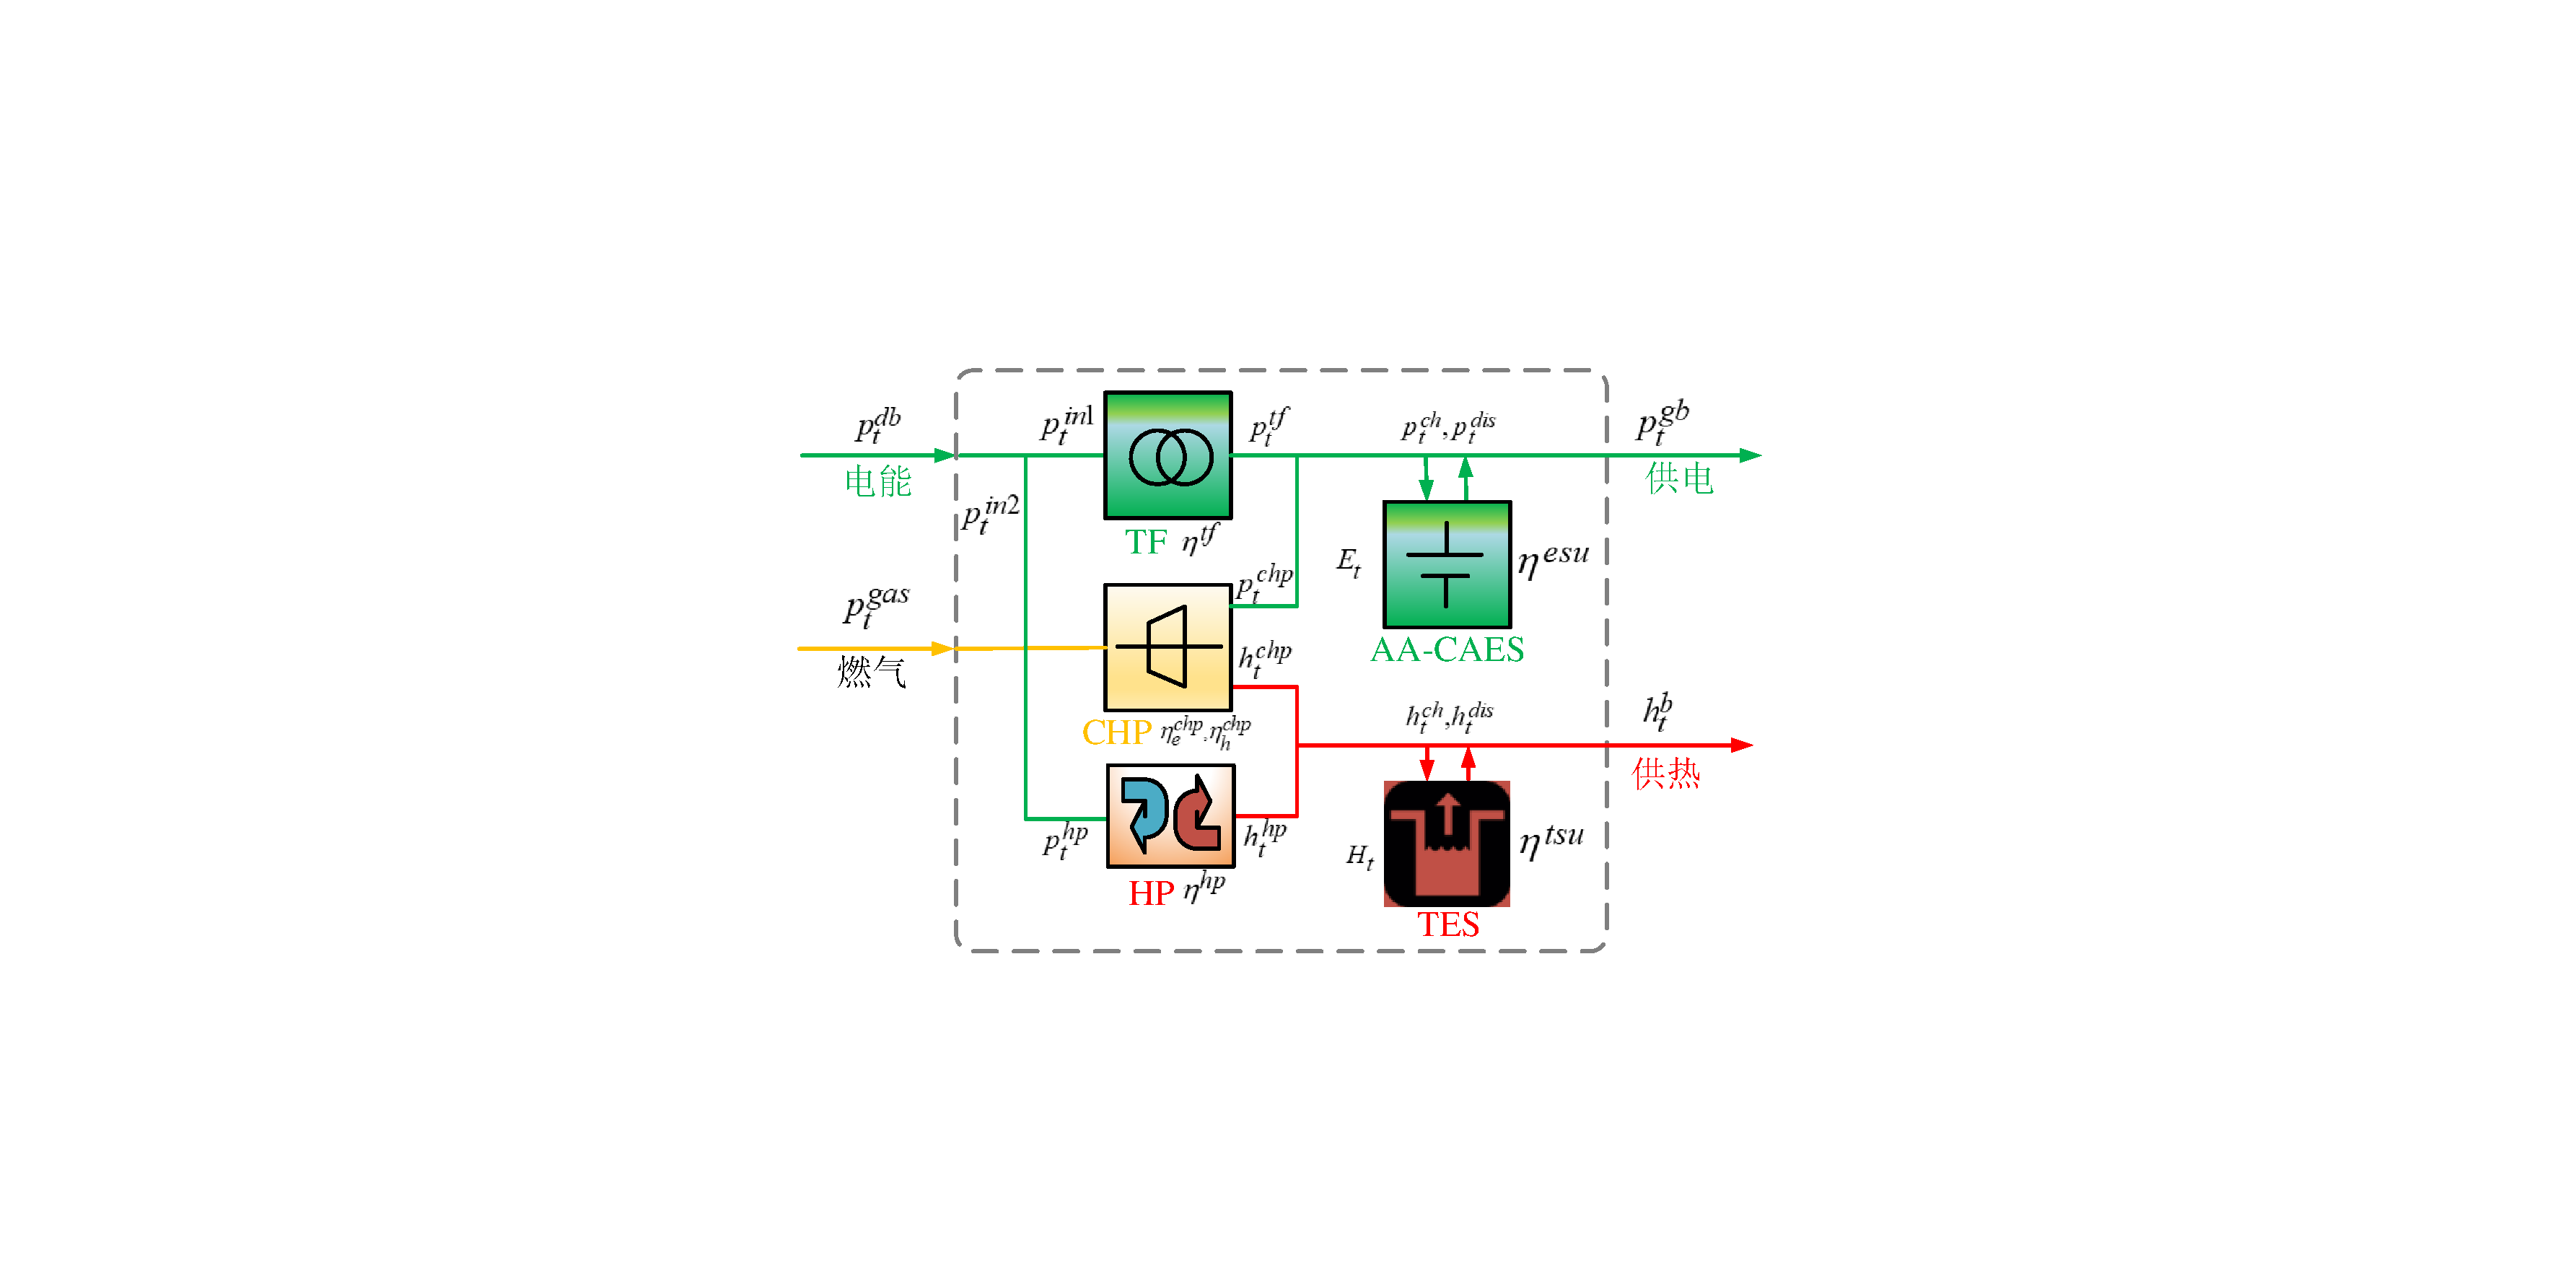
\includegraphics[scale=0.45]{figures/Chap4-2-AA-CAES-Hub-V3.pdf}
  \caption{~II~型AA-CAES能量枢纽结构}
  \label{fig:AA-CAES-Hub-V2}
\end{figure}

II型AA-CAES能量枢纽由于包含燃气与电能两个输入端,对外的供电既可取自电能输入,亦可取自内置的CHP,对外的供热既可取自内置的CHP,亦可取自内置的HP,从而可以充分利用电价、热价及燃料价格信息,实现灵活的内部能量管理;内置储热单元与储电单元的存在,使得II型AA-CAES能量枢纽具有更强的热电供能灵活性。II型能量枢纽基于AA-CAES 的长使用寿命及全生命周期成本优势等将AA-CAES 视为储电部件与CHP等组合形成能量枢纽,主要以第三方主体独立运营。

\subsection{AA-CAES型能量枢纽建模}
\label{sec:thermo-EH-CAES}
%AA-CAES型能量枢纽内含空气压缩机、换热网络、储热系统、储气室、透平发电机组,涉及热动、电动、气动等复杂过程。当前的压缩空气储能系统及能量枢纽建模多采用类似电池等储能系统的简化效率模型,难以刻画AA-CAES能量枢纽内部温度、压强等热动态,无法描述压缩机、透平等组件运行于部分负载工作点导致的变效率现象,无法满足区域热电综合能源系统中能量枢纽的变工况运行要求。
%I型与II型AA-CAES能量枢纽结构的不同,造成了二者不同的应用场景。I型能量枢纽由于内置的储能(储电、储热)单元少,供能灵活性弱于II型能量枢纽,主要用于以集中运行模式管理的园区或社区级热电综合能源系统。该类综合能源系统由于规模小,可实现无碳排运行,其中的所有能源基础设施由统一运营者调配,以充分利用系统中各灵活性分布式电源。与此相反,II型能量枢纽内置的储能单元多,供能灵活性更强,一般以第三方独立运营模式参与到热电综合能源系统的运行。本小节将给出两类能量枢纽的热电联供运行模型。

\textbf{(1) I型AA-CAES能量枢纽}

%本节采用文献~\inlinecite{ST-CAES-CXT-18}中的ST-CAES参数\footnote{由于本章设计的I型AA-CAES不完全等同于ST-CAES,因此对原文献的参数进行了适当修改。}分析本文设计的I 型AA-CAES 能量枢纽的热力学特性。

%此处说明双SOC模型对I型AA-CAES能量枢纽不大适用的问题,但可适用于II型AA-CAES能量枢纽。为此,此处重点针对I型能量枢纽进行热力学热性分析及对应的多能流建模。

在任一时段$t$,能量枢纽中AA-CAES消耗的电功率$W_t^c$由第2章中压缩机额定工况热力学模型(\ref{equ:comp-real-temp-2})-(\ref{equ:comp-pressure})给定,能量枢纽中AA-CAES提供的电功率$W_t^e$ 由第2章中膨胀机额定工况热力学模型(\ref{equ:turb-real-temp-2})-(\ref{equ:turb-pressure})给定。

对于用于区域综合能源系统的I型AA-CAES能量枢纽而言,其储气库一般会采用压力容器,储气库的温度会通过保温措施维持恒定。因此,储气库模型可以采用第\ref{cha:simulation}章中的VT模型(\ref{equ:Air-tank-model-VT}),即任一时刻$t$中储气库的储气压力SOC可以描述为,
\begin{subequations}
\label{eq:hub-pressure-SOC}
\begin{gather}
p_{t + 1}^{as} = p_{t}^{as} + \frac{1}{V_{as}}{R_g}T_t^{as}\left( {u_{t}^c \dot m_{t}^c - u_{t}^e \dot m_{t}^e} \right),\forall t\\
p_{min}^{as} \le p_{t}^{as} \le p_{max}^{as},\forall t
\end{gather}
\end{subequations}
其中,$p_{t}^{as}$ 为储气库压力水平;$T_t^{as}$ 为储气库内空气温度;$u_t^c$与$u_t^e$分别为表示压缩储能与膨胀释能运行状态的布尔量;其它变量或参数已在前文相关章节中定义\footnote{第3章至第5章主要研究面向电力系统运行的AA-CAES,需引入表示运行时段的角标$t$,导致相关变量的命名复杂。为简化变量符号,在不引起混淆的情况下,本章允许对变量上下标的相对位置做了适当调换。}。

相应地,储热水平可由(\ref{equ:TES-HTF-temp})简化为,
\begin{subequations}
\label{eq:hub-thermal-SOC}
\begin{gather}
H_{t}^{TES} = H_{t - 1}^{TES}(1-\gamma_H) + u_{t}^c h_{t}^c - u_{t}^e h_{t}^e - h_{t}^g,\forall t \label{eq:hub-thermal-SOC-Eq}\\
H_{min}^{TES} \le H_{t}^{TES} \le H_{max}^{TES},\forall t
\end{gather}
\end{subequations}
其中,$h_t^c$与$h^e$分别为压缩储能阶段的产热功率与膨胀释能阶段的耗热功率;$h_t^g$为AA-CAES为能量枢纽提供的对外供热功率。由电热泵提供的热功率为,
\begin{equation}
\label{equ:model-HP}
h_{t}^{hp} = \eta_{hp}d_{t}^{hp} \\
\end{equation}
其中,$h_{t}^{hp}$为热泵为能量枢纽提供的对外供热功率;$d_{t}^{hp}$为热泵消耗的电功率;$\eta_{hp}$为热泵效率。

事实上,I型AA-CAES能量枢纽的气热双储双SOC模型(\ref{eq:hub-pressure-SOC})及(\ref{eq:hub-thermal-SOC})与第~\ref{cha:aa-caes}章AA-CAES储能电站双SOC运行模型有异曲同工之妙。主要不同之处在于,I型AA-CAES相比于AA-CAES储能电站的容量较小,可采用压力容器等恒温储热模型,而在等温条件下第\ref{cha:aa-caes}章双SOC采用的储气动态与此处的压力动态一一对应。

\textbf{(2)II型AA-CAES能量枢纽}

II型AA-CAES能量枢纽由于内置了储热单元,同时具有燃气输入以及CHP等灵活性组件的支撑,其内部的AA-CAES储电单元受宽工况运行的影响较小,可以采用等效电池模型(或第\ref{cha:aa-caes}章中的双SOC能量模型)刻画运行特性。本节采用等效电池模型进行建模,以突出整个能量枢纽对外的热电联供特性。针对图~\ref{fig:AA-CAES-Hub-V2}所示的II 型AA-CAES能量枢纽,其热电联供运行模型为,
\begin{subequations}
\label{eq:EH-Cons-II}
\begin{gather}
p_t^{gb} = p_t^{in1} + p_t^{gas} \eta^{chp}_e + p_t^{dis} - p_t^{ch},~ \forall t  \label{eq:EH-Balance-P} \\
h_t^{b} = p_t^{in2} \eta^{hp} + p_t^{gas} \eta^{chp}_h + h_t^{dis} - h_t^{ch},~ \forall t  \label{eq:EH-Balance-H} \\
p_t^{db} = p_t^{in1} + p_t^{in2},~ \forall t  \label{eq:EH-Input} \\
E_{t+1} = E_t + p_t^{ch} \eta^{esu}_+ - p_t^{dis}/\eta^{esu}_-,~\forall t \label{eq:EH-ESU-SOC} \\
H_{t+1} = H_t + h_t^{ch} \eta^{tsu}_+ - h_t^{dis}/\eta^{tsu}_-,~ \forall t \label{eq:EH-TSU-SOC} \\
\mbox{其它变量上下界}   \label{eq:EH-BND}
\end{gather}
\end{subequations}
其中,$p_t^{gas}$ 表示II型能量枢纽消耗的燃料输入;$p_t^{gb}$与$h_t^b$分别表示能量枢纽对外提供的供电功率与供热功率;$p_t^{db}$ 为能量枢纽的电功率需求;$E_t$ 和$H_t$ 分别表示存储在能量枢纽内部储电单元(AA-CAES)与储热单元(TES)的电能与热能; $p_t^{ch}$ 与 $p_t^{dis}$ 分别表示 II型能量枢纽内置的AA-CAES 的压缩功率与膨胀功率;$h_t^{ch}$ 与 $h_t^{dis}$分别表示II型能量枢纽内置的储热单元的储热功率与供热功率,其它中间变量的物理意义如图~\ref{fig:AA-CAES-Hub-V2}中的标注所示。

式(\ref{eq:EH-Balance-P})与(\ref{eq:EH-Balance-H})分别定义了能量枢纽内部的电功率与热功率平衡\footnote{CHP机组主要有背压式与凝汽式两种,此处为了简化模型,假定II型能量枢纽内部的CHP均为背压式,更详细的CHP建模可参见第\ref{sec:ca-wt-power-energy-pene}节及附录
\ref{cha:cons-flexibility-CHP-Thermal}。};(\ref{eq:EH-Input}) 确定了能量枢纽的电功率需求;内置的AA-CAES 储电单元与储热单元的荷电状态(SOC) 由(\ref{eq:EH-ESU-SOC}) 与 (\ref{eq:EH-TSU-SOC}) 描述,假设SOC初态与终态相同,即$E_{T} = E_{0}, H_{T} = H_{0}$;其它中间变量的上下界也由(\ref{eq:EH-BND}) 给定,通过引入相应的布尔量,内置AA-CAES与储热单元不同时充放的约束也放置于(\ref{eq:EH-BND})。

%\subsection{能量枢纽热电可行域}
%
%\subsubsection{I型能量枢纽热电可行域}
%
%\subsubsection{II型能量枢纽热电可行域}

\section{含能量枢纽的热电综合能源系统的调度运行}
\label{sec:st-caes-dispatch}

本节在区域供热网络与区域配电网及能量枢纽均由统一的综合能源集成运营商负责的假设下,研究含能量枢纽的区域热电综合能源系统的经济调度问题。这种集中运营假设在区域级或社区级系统中一般成立,如Aalborg CSP公司开展的区域级多能互补系统~\footnote{https://www.aalborgcsp.com/projects/project-overview/}, Aalborg 大学开展的智慧能源系统~\cite{Smart-Energy-Systems-15},以及清华-青海大学开展的以光热复合压缩空气储能为能量枢纽的智慧微能源网~\cite{ST-CAES-CN-16-Rui, ST-CAES-17}。

区域热电综合能源系统一般采用能量枢纽实现区域配电网(Power Distribution Network,PDN)与区域供热网络(District Heating Network,DHN)的耦合,为此我们采用DistFlow 刻画区域配电网潮流模型,并用水力-热力模型描述区域供热网络潮流分布。此外,该类区域综合能源系统多为零碳排系统,本节最后基于IEEE33节点PDN 和8 节点DHN 构建的典型零碳排热电综合能源系统的算例,验证AA-CAES能量枢纽具有的供能灵活性对提升可再生能源消纳水平、降低区域热电综合能源系统整体运行成本等方面的益处。第\ref{sec:bid-st-caes}节将针对能量枢纽、区域配电网、供热网络由不同运营商管理的假设,研究能量枢纽的市场运营问题。

\subsection{区域供热网络潮流模型}
\label{sec:st-case-dispatch-DHN}
区域供热网络通常由热源、热负荷及具有相同拓扑结构的供水网络与回水网络组成,如图~\ref{Fig:DHN-Topology}~所示。我们采用由热力分布和水力分布构成的工质流模型描述供回水温度、质量流率等热网潮流信息,其热力分布可建模为\cite{LXZ-DHN-2016, DHN-Model-17},
\begin{subequations}
\label{eq:DHN-Thermal-Part}
\begin{gather}
\sum\limits_{b \in T(i)} {({\tau _{b,t}^{S,out}\dot m_{b,t}^S})}  = \tau _{i,t}^S\sum\limits_{b \in T(i)}{\dot m_{b,t}^S} ,\forall i,t \label{eq:DHN-Temp-Mix-S}\\
\sum\limits_{b \in F(i)} {({\tau _{b,t}^{R,out}\dot m_{b,t}^R})}  = \tau _{i,t}^R\sum\limits_{b \in F(i)}{\dot m_{b,t}^R} ,\forall i,t\label{eq:DHN-Temp-Mix-R}\\
\tau _{b,t}^{S,in} = \tau _{i,t}^S,\tau _{b,t}^{R,in} = \tau _{i,t}^R,\forall i,b,t \label{eq:DHN-Node-Temp}\\
\tau _{b,t}^{S,out} = ({\tau _{b,t}^{S,in} - \tau _t^{am}}){e^{-\frac{{{\lambda _b} {l_b}}}{{{c_p} \dot m_{b,t}^S}}}} + \tau _t^{am},\forall b,t\label{eq:DHN-Pipe-Loss-S}\\
\tau _{b,t}^{R,out} = ({\tau _{b,t}^{R,in} - \tau _t^{am}}){e^{ - \frac{{{\lambda _b}{l_b}}}{{{c_p}\dot m_{b,t}^R}}}} + \tau _t^{am},\forall b,t \label{eq:DHN-Pipe-Loss-R}
\end{gather}
\end{subequations}
其中,${c_p}$ 为载热工质(水)比热容;$\tau _{b,t}^{S,out}$,$\tau _{b,t}^{S,in}$,$\tau _{b,t}^{R,out}$,$\tau _{b,t}^{R,in}$ 分别为供回水管网出口及入口温度,表征供热管网热力工况;$\dot m_{b,t}^S$与$\dot m_{b,t}^R$分别为流经供回水管网的载热流体质量流率,表征供热管网水力工况;下标$b$表示管道编号,$t$表示运行时段;上标S与R分别表示供水侧与回水侧,in与out分别表示管道的入口与出口;$T(i)$ 与$F(i)$分别表示以节点$i$为末节点与首节点的管道集合;$\lambda_b$为管道$b$的温度损耗系数;$l_b$ 为管道$b$ 的长度。(\ref{eq:DHN-Temp-Mix-S}) 与(\ref{eq:DHN-Temp-Mix-R}) 分别表示供水侧及回水侧的节点温度混合(能量守恒)方程;(\ref{eq:DHN-Node-Temp}) 表示供回水管网节点温度;(\ref{eq:DHN-Pipe-Loss-S})与(\ref{eq:DHN-Pipe-Loss-R})分别表示工质经过供水侧与回水侧管网引起的温度损耗。

\begin{figure}[H]
\centering
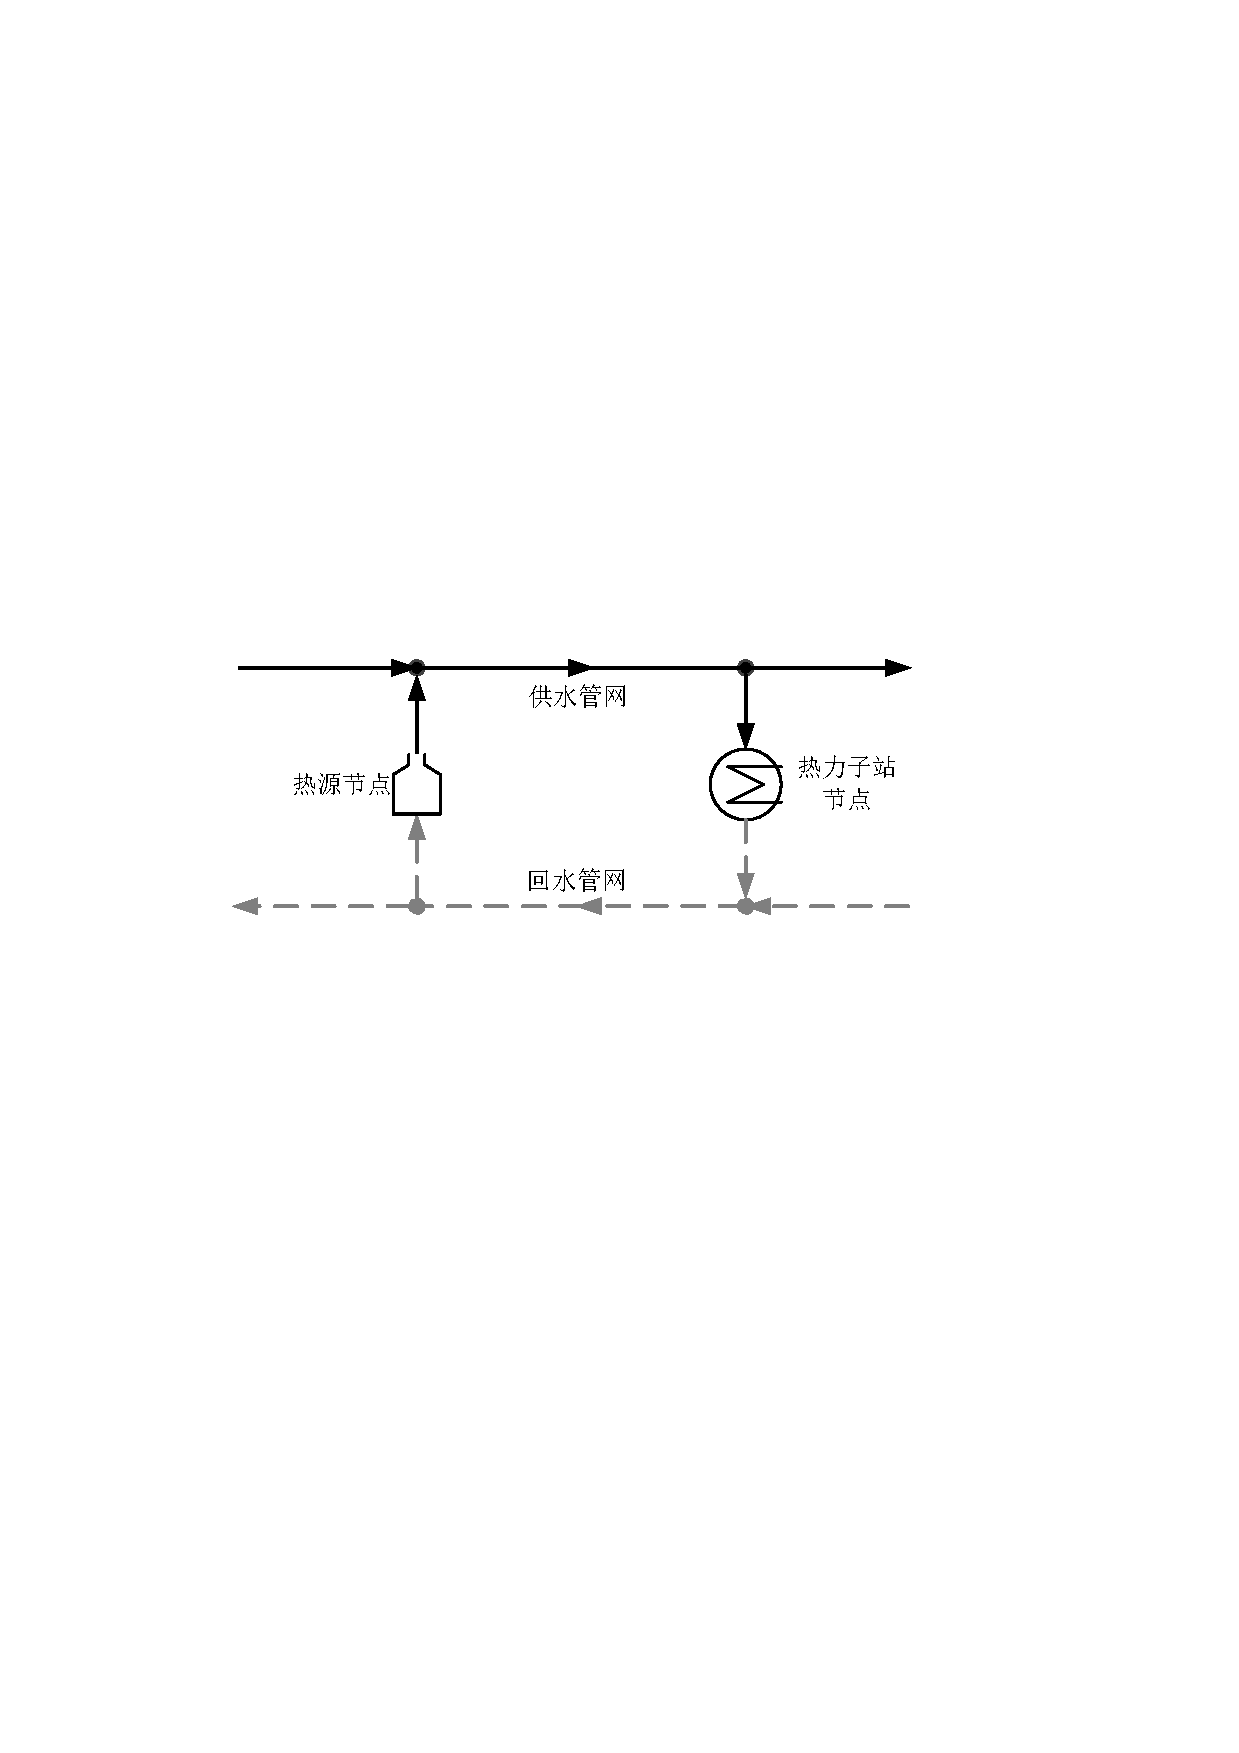
\includegraphics[scale=0.75]{figures/Chap4-3-DHN-Energy-Topo.pdf}
\caption{区域供热网络结构示意图}
\label{Fig:DHN-Topology}
\end{figure}

质量流率(水力分布)可通过质量守恒约束确定\cite{LXZ-DHN-2016, DHN-Model-17},
\begin{subequations}
\label{eq:DHN-Hydra-Part}
\begin{gather}
\sum\limits_{b \in F(i)} {\dot m_{b,t}^S}  + \dot m_{i,t}^d = \dot m_{i,t}^g + \sum\limits_{b \in T(i)} {\dot m_{b,t}^S} ,\forall i,t \label{eq:DHN-Hydra-Part-S}\\
\sum\limits_{b \in F(i)} {\dot m_{b,t}^R}  + \dot m_{i,t}^g = \dot m_{i,t}^d + \sum\limits_{b \in T(i)} {\dot m_{b,t}^R} ,\forall i,t \label{eq:DHN-Hydra-Part-R}\\
0 \le \dot m_{b,t}^S \le \dot m_b^u,0 \le \dot m_{b,t}^R \le \dot m_b^u,\forall b,t\label{eq:DHN-Hydra-Part-Limit}
%\tau^{out} = (\tau^{in}-\tau^{am}){\rm e}^{-\lambda_b l_b/c_p \dot m} + \tau^{am} \label{eq:DHN-Pipe-Loss} \\
%\tau^{mix} = \dfrac{\sum_{b \in L_E(i)} (\tau_b^{out} \dot m_b)}{\sum_{b \in L_E(i)} \dot m_{b}} \label{eq:DHN-Mix-Temp-1} \\
%\tau^{in}_b = \tau^{mix},~ \forall b \in L_B(i)\label{eq:DHN-Mix-Temp-2} \\
%\tau^{out}_b = \tau^{in}_{b'},~ \forall b \in L_E(i),~ \forall b' \in L_B(i)\label{eq:DHN-Mix-Temp-3}
\end{gather}
\end{subequations}
其中,$\dot m_{i,t}^g$与$\dot m_{i,t}^d$分别为节点$i$热源(如AA-CAES能量枢纽)与热负荷的质量流率;$\dot m_b^u$为管道$b$的质量流率上界。(\ref{eq:DHN-Hydra-Part-S})与(\ref{eq:DHN-Hydra-Part-R})分别表示供水侧与回水侧节点$i$的质量平衡约束;(\ref{eq:DHN-Hydra-Part-Limit})表示管道运行的物理限制。

供热网络中热源与热负荷节点的热功率满足,
\begin{subequations}
\label{eq:DHN-heat-power-model}
\begin{gather}
h_{i,t}^{d} = c_p \dot m_{i,t}^d  (\tau_{i,t}^S - \tau_{i,t}^R), \forall i,t \\
h_{j,t}^{hp} = c_p \dot m_{j,t}^g  (\tau_{j,t}^S - \tau_{j,t}^R), \forall j,t \\
h_{i,t}^{g} = c_p \dot m_{i,t}^g  (\tau_{i,t}^S - \tau_{i,t}^R), \forall i,t
\end{gather}
\end{subequations}
%h = c_p \dot m (\tau^S - \tau^R) \label{eq:DHN-Heat-Exchange}\\
其中,$h_{i,t}^d$为热负荷的热功率需求;$h_{j,t}^{hp}$为热泵提供的热功率,且由(\ref{equ:model-HP})决定;$h_{i,t}^g$为其它热源的供热功率。

\subsection{区域配电网络潮流模型}
\label{sec:st-case-dispatch-PDN}
区域供电网络一般为辐射式结构, 如图~\ref{Fig:PDN-Topology}~所示,可采用Dist Flow潮流模型进行建模为\cite{Distflow-WFL, Branchflow-SH1},
\begin{subequations}
\label{eq:PDN-Branch-Flow-All}
\begin{gather}
P_{ij,t} + p_{j,t}^g + W_{j,t}^e - r_{ij}I_{ij,t} = \sum\limits_{k \in \pi(j)} {P_{jk,t}}+ p_{j,t}^d +  W_{j,t}^c + d_{j,t}^{hp},\forall l({i,j}),t \label{eq:PDN-Node-Balance-P}\\
Q_{ij,t} + q_{j,t}^g - x_{ij}I_{ij,t} = \sum\limits_{k \in \pi(j)} {{Q_{jk,t}}}+ q_{j,t}^d,\forall l({i,j}),t \label{eq:PDN-Node-Balance-Q}\\
{U_{j,t}} = {U_{i,t}}-2({{r_{ij}}P_{ij,t} + x_{ij}{Q_{ij,t}}}) + {({{z_{ij}}})^2}{I_{ij,t}},\forall l({i,j}),t \label{eq:PDN-Node-Balance-U}\\
{I_{ij,t}}{U_{i,t}} = {P_{ij,t}}^2 + Q{_{ij,t}^2},\forall l({i,j}),t \label{eq:PDN-Relation-PQ}\\
I_{ij,t} \le I_{ij}^u,U_i^l \le {U_{i,t}} \le U_i^u,\forall i,l({i,j}),t \label{eq:PDN-Limit-UI}\\
p_{i,t}^l \le p_{i,t}^g \le p_i^u,q_i^l \le q_{i,t}^g \le q_i^u,\forall i,t \label{eq:PDN-Limit-PQ}
\end{gather}
\end{subequations}
其中,$P_{ij,t}$与${Q_{ij,t}}$分别为线路的传输有功与无功功率;$p_{j,t}^d$与$q_{j,t}^d$分别为节点$j$的有功与无功功率需求;$p_{j,t}^g$与$q_{j,t}^g$分别为各电源(分布式可再生能源机组、燃气轮机等)有功与无功出力\footnote{文献\inlinecite{CAES-Reactive-18-LGK}指出AA-CAES具有一定的无功支撑能力,本文在此假定其不提供无功,但相关建模分析方法完全适用于考虑其提供无功的场景。};$W_{j,t}^e$,$W_{j,t}^c$,$d_{j,t}^{hp}$分别为I型AA-CAES热电能量枢纽(图
\ref{fig:AA-CAES-Hub-V1})与电网的(电)功率接口;$\pi(j)$ 为节点$j$ 的子节点集合;${x_{ij}},{r_{ij}},{z_{ij}}$ 代表线路电抗、电阻及阻抗;${U_{j,t}}$ 为节点电压幅值$V_{j,t}$的平方;${I_{ij}}$ 为线路电流的平方;上标u与l分别表示上界与下界。(\ref{eq:PDN-Node-Balance-P})与(\ref{eq:PDN-Node-Balance-Q})分别表示节点有功和无功功率平衡方程,若系统中存在风电等其它电源,只需进行相应即可;(\ref{eq:PDN-Node-Balance-U}) 定义节点电压幅值;(\ref{eq:PDN-Relation-PQ})给出线路有功与无功与节点电压及线路电流间的耦合关系;(\ref{eq:PDN-Limit-UI}) 与(\ref{eq:PDN-Limit-PQ})给出各物理量的实际物理限制。

\begin{figure}[H]
\centering
\includegraphics[scale=0.89]{Fig-2-PDN-Topology}
\caption{辐射状配电网结构示意图}
\label{Fig:PDN-Topology}
\end{figure}

Dist Flow模型(\ref{eq:PDN-Branch-Flow-All})描述了热电综合能源系统中的(电功率)潮流分布,其优势在于可以给出节点电压、线路无功等配电网中较为关注的运行信息,同时该模型可被线性化或凸松弛化(如二阶锥松弛\cite{Thesis-Liubin})以高效求解。例如,线性化的DistFlow模型为\cite{BFM-Lin-1,BFM-Lin-2},
\begin{subequations}
\label{eq:Lin-Dist-Flow-Non-OLTC}
\begin{gather}
P_{ij,t} + p_{j,t}^g + W_{j,t}^e = \sum_{k \in \pi(j)} P_{jk,t} + W_{j,t}^c + p_{j,t}^d + d_{j,t}^{hp}, \forall l(i,j),t \label{eq:PF-P} \\
Q_{ij,t} + q_{j,t}^g = \sum_{k \in \pi(j)} Q_{jk,t} + q_{j,t}^d, \forall l(i,j),t \label{eq:PF-Q} \\
U_{j,t} = U_{i,t} - ({r_{ij} P_{ij,t} + x_{ij} Q_{ij,t}}){U_0}, \forall j,t \label{eq:PF-U} \\
U_i^l \le {U_{i,t}} \le U_i^u,\forall i,{U_0} = V_{sl}^2 , \forall i,t \\
p_i^l \le p_{i,t}^g \le p_i^u,q_i^l \le q_{i,t}^g \le q_i^u, \forall i,t
\end{gather}
\end{subequations}
其中,$V_{sl}$为平衡节点的电压幅值,对于辐射状PDN一般为馈入节点的电压幅值。

%特别地,当线路含有离散电容器组进行无功补偿时,(\ref{eq:PF-Q})可修正为
%\begin{equation}
%{Q_{ij,t}} + q_{j,t}^g + \frac{{{U_{j,t}}{C_j}}}{2} + {Q_{cj,t}} - {x_{ij}}{i_{ij,t}} = \sum\limits_{k \in \pi \left( j \right)} {{Q_{jk,t}}}  + q_{j,t}^d,\forall t
%\end{equation}
%
%若配电网中无离散的电容器组等无功补偿装置及OLTC等调节装置时,配电网潮流模型可退化为

对于实际运行的配电网而言,为了维持较好的电压质量,一般会增设连续无功补偿装置(如SVG)、离散的电容器组以及有载调压变压器(OLTC)等。为此,可在线性化DistFlow 模型(\ref{eq:Lin-Dist-Flow-Non-OLTC})的基础上,修正含离散电容器或连续无功补偿装置以及含OLTC线路的无功平衡方程(\ref{eq:PF-Q})与节点电压方程(\ref{eq:PF-U})为\cite{PDN-Model-Reactive-Power-DT-16, CAES-IES-16-Rui},
\begin{subequations}
\label{eq:Lin-Dist-Flow-Plus-OLTC}
\begin{gather}
{Q_{ij,t}} + q_{j,t}^g + \frac{{{U_{j,t}}{C_{j,t}}}}{2} + {q_{j,t}^c} = \sum\limits_{k \in \pi \left( j \right)} {{Q_{jk,t}}}  + q_{j,t}^d,\forall t \label{eq:Lin-Dist-Flow-Plus-OLTC-1}\\
\frac{{{U_{j,t}}}}{{K_{ij,t}^2}} = {U_{i,t}} - \left( {{r_{ij}}{P_{ij,t}} + {x_{ij}}{Q_{ij,t}}} \right)/{U_0},\forall t\label{eq:Lin-Dist-Flow-Plus-OLTC-2}
\end{gather}
\end{subequations}
其中,${C_{j,t}}$为投运的电容或电抗器值; $q_{j,t}^{c}$为连续无功补偿量;$K_{ij,t}^{}$ 为OLTC变比。

\subsection{含~AA-CAES~能量枢纽的热电系统调度模型}

在集中运营模式下,假定无碳排区域热电综合能源系统中的负荷由风电机组与上级电网承担,热能由I型AA-CAES热电能量枢纽提供,系统调度以最小化系统运行成本为目标,即
\begin{subequations}
\label{eq:CAES-Hub-dispatch}
\begin{gather}
\min \;\;\sum\limits_{t \in T} {{\lambda_t}{p_{0,t}^g}} \label{eq:CAES-Hub-dispatch-obj}\\
\mbox{s.t.}~
\mbox{I型AA-CAES能量枢纽热电联供模型}\\
\mbox{PDN线性DistFlow模型}\\
\mbox{供热网络热力-水力潮流模型} \\
W_i^{g,l} \le W_{i,t}^g \le W_i^{g,u},\forall i,t
\end{gather}
\end{subequations}
其中,${\lambda_t}$为电价;${p_{0,t}^g}$为区域热电综合能源系统从上级电网中购入的电功率;$W_{i,t}^g$为风电机组实际出力,$W_i^{g,l}$ 与$W_i^{g,u}$分别为风电出力最小值与预测值。

无碳排调度模型(\ref{eq:CAES-Hub-dispatch})为非线性优化问题,其非线性主要源自配电网潮流模型及供热网络潮流模型,本小节将分别给出相应的线性化方法,以在不丢失准确性的同时将模型转化为易于高效求解的MILP问题。事实上,OLTC、电容/电抗器组等离散型无功补偿装置的调节或投切亦存在相应的运行成本,目标函数(\ref{eq:CAES-Hub-dispatch-obj})中可进一步扩展至考虑无功补偿成本,相关的线性化及求解方法也基本适用。

\subsubsection{配电网潮流模型的线性化}
改进的区域配电网潮流模型(\ref{eq:Lin-Dist-Flow-Non-OLTC})-(\ref{eq:Lin-Dist-Flow-Plus-OLTC}) 中的非线性主要源自离散电容器组引起的非线性项${U_{j,t}}{C_j}/2$与OLTC变比调节引入的非线性项${{{U_{j,t}}}}/{{K_{ij,t}^2}}$。类似于\ref{sec:chap3-bid-aa-caes}节中的布尔展开法,非线性项${U_{j,t}}{C_j}/2$中的离散量$C_j$可线性化为\cite{PDN-Model-Reactive-Power-DT-16, CAES-IES-16-Rui},
\begin{subequations}
\begin{gather}
\label{eq:UC-approx}
{{C_j} = C_j^l + {s_j}({{2^0}{g_{j,0}} + {2^1}{g_{j,1}} + \cdots + {2^{{v_j}}}{g_{j,{v_j}}}})}, {{g_{j,0}},{g_{j,1}}, \cdots ,{g_{j,{v_j}}} \in \{ 0,1\} }\\
{0 \le {2^0}{g_{j,0}} + {2^1}{g_{j,1}} +  \cdots  + {2^{{v_j}}}{g_{j,{v_j}}} \le ({C_j^u - C_j^l})/{s_j},}{\forall j \in {E_D}}
\end{gather}
\end{subequations}
其中,$C_j^l$与$C_j^u$分别为电容器或电抗器容量的最小值与最大值;${s_j}$ 为电容器或电抗器的步进容量;${E_D}$ 为增设电容器或电抗器的母线集合;整数变量$v_j$ 表征离散化段数,可由下式决定
\begin{equation}
{\log _2}({\frac{{C_j^u - C_j^l}}{{{s_j}}} + 1})-1 \le {v_j} \le {\log _2}({\frac{{C_j^u - C_j^l}}{{{s_j}}} + 1})
\end{equation}
因此,非线性项${U_{j,t}}{C_{j,t}}$可转化为,
\begin{equation}
\label{eq:UC-approx-2}
{U_{j,t}}{C_{j,t}} = C_j^l{U_{j,t}} + {s_j}({{2^0}{\delta _{j,0}} +  \cdots  + {2^{{v_j}}}{\delta _{j,{v_j}}}})
\end{equation}
进一步,式(\ref{eq:UC-approx-2})可用大M法\cite{Big-M-1981} 线性化,即
\begin{subequations}
\label{eq:UC-approx-final}
\begin{gather}
%{{U_{j,t}}{C_{j,t}} = C_j^l{U_{j,t}} + {s_j}\left( {{2^0}{\delta _{j,0}} +  \cdots  + {2^{{v_j}}}{\delta _{j,{v_j}}}} \right)}\\
{{U_{j,t}} - M({1 - {g_{j,k,t}}}) \le {\delta _{j,k,t}} \le {U_{j,t}} + M({1 - {g_{j,k,t}}})}\\
{ - M{g_{j,k,t}} \le {\delta _{j,k,t}} \le M{g_{j,k,t}}}
\end{gather}
\end{subequations}
其中,${\delta _{j,k,t}}$为辅助的连续量;M为一足够大的正数。

针对含有载调压器~OLTC~的支路~$l(i,j)$,其无功功率约束(\ref{eq:Lin-Dist-Flow-Plus-OLTC-2})可线性化为,
\begin{equation}
\label{eq:OLTC-approxi-1}
\frac{{{U_{j,t}}}}{{K_{ij,t}^2}} = {U_{j,t}}({\frac{{{b_{ij,1,t}}}}{{K_{ij,1}^2}} + \frac{{{b_{ij,2,t}}}}{{K_{ij,2}^2}}{\rm{ + }} \cdots {\rm{ + }}\frac{{{b_{ij,{n_{ij}},t}}}}{{K_{ij,{n_{ij}}}^2}}})
\end{equation}
其中,$K_{ij,1}^{}$, $K_{ij,2}^{}$, ..., $K_{ij,{n_{ij}}}^{}$ 为增设于线路$l(i,j)$ 的OLTC变比的可能取值;${n_{ij}}$为相应的变比离散取值个数。

综上,含OLTC的节点电压约束(\ref{eq:Lin-Dist-Flow-Plus-OLTC-2})可线性化为\cite{PDN-Model-Reactive-Power-14, PDN-Model-Reactive-Power-DT-16, CAES-IES-16-Rui},
\begin{subequations}
\label{eq:OLTC-approxi-2}
\begin{gather}
{{U_{j,t}}/K_{ij,t}^2 = \sum\limits_{k = 1}^{{n_{ij}}} {{h_{j,k,t}}/K_{ij,k}^2} }\\
{{b_{ij,1,t}}, \cdots ,{b_{ij,{n_{ij}},t}} \in \{ 0,1\} ,\sum\limits_{k = 1}^{{n_{ij}}} {{b_{j,k,t}}}  = 1}\\
{ - M({1 - {b_{ij,k,t}}}) + {U_{j,t}} \le {h_{j,k,t}} \le M({1 - {b_{ij,k,t}}}) + {U_{j,t}}}\\
{ - M{b_{ij,k,t}} \le {h_{j,k,t}} \le M{b_{ij,k,t}}}
\end{gather}
\end{subequations}
其中,$h_{j,k,t}$为辅助的连续变量。

\subsubsection{区域热网潮流模型的线性化}
%热网模型(\ref{eq:DHN-Thermal-Part})-(\ref{eq:DHN-Hydra-Part})采用耦合的水力和热力模型描述热网中工质的水力工况(压强、质量流率)和热力工况(供回水温度), 模型较为复杂。

区域供热网络存在两种调节方式,即CF-VT与VF-VT\cite{DHN-CFVT-2013},前者通过固定质量流率调节供(回)水温度来满足供热负荷随外界温度的变化需求,而后者通过质量流率和供(回)水温度的共同调节来满足日供热负荷需求。

由(\ref{eq:DHN-heat-power-model})可知,当日供热负荷波动范围较大时,仅靠温度的调节往往不能满足供热负荷需求,加之供热管道温度半动态的存在导致温度调节的响应存在时延\cite{IES-DHN-16-LZG},调节灵活性与及时性往往不高。因此,CF-VT模式存在一定局限性。质量流率调节响应速度快,可为供热负荷的调节带来更高的灵活性,使得VF-VT 模式具备更大的灵活性。然而,VF-VT 模式下水力工况和热力工况耦合性强,模型求解较为困难。实际运行中一般先计算水力分布,确定工质质量流率,进而进行CF-VT 调节。因此,我们假定日内热负荷的调整仅通过CF-VT模式实现,即$\dot m$已知,从而非线性模型(\ref{eq:DHN-Thermal-Part})(\ref{eq:DHN-Hydra-Part})退化为线性模型。

\subsection{集中运营热电综合能源系统算例分析}
本小节分析含图~\ref{fig:AA-CAES-Hub-V1}所示的I型~AA-CAES~ 能量枢纽的零碳排区域热电综合能源系统的最优调度。算例中的仿真由配有i5-4210M CPU 与16 GB RAM 的计算单元完成,模型采用YALMIP\cite{YALMIP}建模,求解器为CPLEX\footnote{具体代码可参见https://github.com/AIRicky/Integrated-Energy-Systems-with-CAES}。

\subsubsection{算例设置}
采用图\ref{Fig:Hub-Dispatch-Exe-PDN33DHN8}所示的测试系统模拟园区级或区域级无碳排热电综合能源系统,该系统由33节点PDN、8节点DHN、I型AA-CAES能量枢纽、4台风机组成。母线2处含一座容量为3MW(6台0.5MW风机组成)的小型风电场,其它母线处的风机容量均为0.5MW。

\begin{figure}[H]
\centering
\includegraphics[scale=0.80]{figures/Chap4-15-Hub-Dispatch-Exe-PDN33DHN8-V2.pdf}
\caption{集中运营环境下的区域热电综合能源测试系统}
\label{Fig:Hub-Dispatch-Exe-PDN33DHN8}
\end{figure}

\begin{figure}[H]
\centering
\includegraphics[scale=0.60]{figures/Chap4-15-Hub-Dispatch-Exe-TOU.pdf}
\caption{分时电价曲线}
\label{Fig:Hub-Dispatch-Exe-TOU}
\end{figure}

鉴于该类无碳排园区级热电综合能源系统在我国较为常见,此处采用图~\ref{Fig:Hub-Dispatch-Exe-TOU}所示的电力市场分时电价曲线。对于实时电价等美国电力批发市场较为常见的价格机制,我们将在第~\ref{sec:bid-st-caes}节独立运营模式下的AA-CAES能量枢纽的市场竞标问题中进行讨论。系统中所有风电机组的总功率预测曲线(各风机按容量分配)、总电负荷及热负荷需求如图~\ref{Fig:Hub-Dispatch-Exe-PQWHG} 所示,电网各母线负荷分配比例由MATPOWER 33 节点配电网标准潮流~\cite{MATPOWER} 求得, 热网各节点热负荷分配比例及质量流率见表\ref{tab:para-thermo-load}。

\begin{figure}[H]
\centering
\includegraphics[scale=0.81]{figures/Chap4-15-Hub-Dispatch-Exe-PQWHG.pdf}
\caption{负荷需求与风电预测功率}
\label{Fig:Hub-Dispatch-Exe-PQWHG}
\end{figure}

\begin{table}[htb]
  \centering
  \begin{minipage}[t]{0.65\linewidth} % 如果想在表格中使用脚注,minipage是个不错的办法
  \caption{8节点区域热网节点参数}
  \label{tab:para-thermo-load}
    \begin{tabularx}{\linewidth}{ccccccccc}
      \toprule[1.5pt]
      {\heiti 节点编号} & {\heiti \#1} & {\heiti \#2} &  {\heiti \#3} & {\heiti \#4} & {\heiti \#5} & {\heiti \#6} & {\heiti \#7} & {\heiti \#8} \\\midrule[1pt]
      负荷比例 (\%)& 0  & 0 & 0	& 0	& 20 & 20 & 20 & 40\\
      质量流率 (kg/s)& 10	& 0	& 0	& 0	& 2	  & 2   & 2	  & 4\\
      \bottomrule[1.5pt]
    \end{tabularx}
  \end{minipage}
\end{table}

为了维持配电网中各母线的电压质量,在配电网各中枢节点部署了无功补偿装置。参考文献\inlinecite{Thesis-Liubin}中的系统设置,在线路\#1, \#18, \#22, \#25 上装设最小分接头为0.95,最大分接头为1.05 以及分接头步长为0.01的OLTC\cite{Thesis-Liubin}。并联电容器装设于母线 \#5, \#10, \#13, \#17, \#20, \#23, \#30,其容量范围为0-0.2,调节步长为~0.05。此外,SVG增设于母线~\#4, \#9, \#14,以提供连续无功补偿。

\subsubsection{能量枢纽仿真}
本小节先仿真分析I型能量枢纽内部的AA-CAES在一个循环周期内的能量平衡情况,为分析其在热电综合能源系统中的供能特性提供参考。内置的AA-CAES采用两级压缩两级膨胀结构,采用常压-常压运行方式及热电联供供能模式,储气库的工作压力范围为8.4 MPa-9.0 MPa。由于常压-常压运行模式的设定,储气库的压力变化对压缩机与膨胀机的部分负载运行影响不大。同时,储气库的压力工作范围较窄,温度变化也不大。压缩机与膨胀机的额定质量流率分别为0.64 kg/s, 2.46 kg/s,其它参数分别如表\ref{tab:para-comp-energy-hub-dispatch}及表\ref{tab:para-turb-energy-hub-dispatch}所示,储气库体积为 2000 m$^3$。

\begin{table}[htb]
  \centering
  \begin{minipage}[t]{0.85\linewidth} % 如果想在表格中使用脚注,minipage是个不错的办法
  \caption{压缩机额定参数}
  \label{tab:para-comp-energy-hub-dispatch}
    \begin{tabularx}{\linewidth}{ccccccc}
      \toprule[1.5pt]
      {\heiti 级数} &  {\heiti 进口压力 } & {\heiti 出口压力} & 进口温度 &  出口温度 & 额定功率 & 等熵效率 \\\midrule[1pt]
       一级  & 0.1 MPa  & 1.15 MPa & 15	$^\circ$C & 375 $^\circ$C &	250 kW & 0.85 \\
       二级  & 1.15 MPa & 9	 MPa  & 40 $^\circ$C  & 366 $^\circ$C & 250 kW & 0.81 \\
      \bottomrule[1.5pt]
    \end{tabularx}
  \end{minipage}
\end{table}

\begin{table}[htb]
  \centering
  \begin{minipage}[t]{0.85\linewidth} % 如果想在表格中使用脚注,minipage是个不错的办法
  \caption{膨胀机额定参数}
  \label{tab:para-turb-energy-hub-dispatch}
    \begin{tabularx}{\linewidth}{ccccccc}
      \toprule[1.5pt]
      {\heiti 级数} &  {\heiti 进口压力} & {\heiti 出口压力} & 进口温度 &  出口温度 & 额定功率 & 等熵效率 \\\midrule[1pt]
      一级  & 8.4 MPa  & 0.94 MPa & 280 $^\circ$C & 60 $^\circ$C  & 500 kW & 0.82 \\
      二级  & 0.94 MPa & 1 MPa    & 280 $^\circ$C & 60 $^\circ$C  & 500 kW & 0.82 \\
      \bottomrule[1.5pt]
    \end{tabularx}
  \end{minipage}
\end{table}

在上述设定下,基于第\ref{cha:simulation}章热力学仿真模型得出一个循环周期内I型能量枢纽内部AA-CAES的能量平衡如图~\ref{Fig:Hub-Dispatch-AA-CAES-Flow}所示,其电-电转换效率为${\eta _{elec}}$ = 1.46/2.8 = 52.14\%,热效率为$\eta_{heat}$=0.4193/2.8=14.98\%,(热电)总能利用效率为${\eta _{total}}$ =(1.46 + 0.4193)/2.8 = 67.12\%。在合适的电力市场环境下, 该效率值对于AA-CAES 型能量枢纽的商业化运行是可接受的。

\begin{figure}[H]
\centering
\includegraphics[scale=0.65]{figures/Chap4-15-Hub-Dispatch-AA-CAES-Flow-V2.pdf}
\caption{AA-CAES在一个循环周期内的能量平衡}
\label{Fig:Hub-Dispatch-AA-CAES-Flow}
\end{figure}

\subsubsection{结果分析}

(1)AA-CAES能量枢纽

AA-CAES热电多能联供时,储气库储气压力的变化仅由压缩储能消耗与膨胀释能输出的电功率有关,而储热罐中的储热水平不仅与压缩功率及膨胀功率有关,还与当前的供热功率有关。I型能量枢纽中AA-CAES的储气水平与储热水平变化曲线分别如图~\ref{Fig:Hub-Dispatch-Exe-ASU-SOC} 及\ref{Fig:Hub-Dispatch-Exe-TES-SOC}所示。

\begin{figure}[H]
\centering
\includegraphics[scale=0.66]{figures/Chap4-15-Hub-Dispatch-Exe-ASU-SOC-V2.pdf}
\caption{AA-CAES能量枢纽储气水平曲线}
\label{Fig:Hub-Dispatch-Exe-ASU-SOC}
\end{figure}

\begin{figure}[H]
\centering
\includegraphics[scale=0.65]{figures/Chap4-15-Hub-Dispatch-Exe-TES-SOC-V2.pdf}
\caption{AA-CAES能量枢纽储热水平曲线}
\label{Fig:Hub-Dispatch-Exe-TES-SOC}
\end{figure}

I型能量枢纽中AA-CAES在多能联供模式下具有的供能灵活性,使其既可以经典的压缩-储热模式(时段1-时段6)与膨胀-耗热模式(时段13-时段14)运行,以实现电能“缓存”与“搬移”,又可运行于静置-供热模式(时段10、时段16)与压缩-供热模式(时段24),从而为区域热电综合能源系统注入运行灵活性。在当前的系统设定下,压缩机可以实现高负载或额定功率运行来减小购电成本,而膨胀机则在部分时段(时段13)以部分负载方式发电,消耗低谷时段存储的低价电能,以降低热电综合能源系统总体运行成本。

此外,由图~\ref{Fig:Hub-Dispatch-Exe-ASU-SOC}及图\ref{Fig:Hub-Dispatch-Exe-TES-SOC}可以看出,实际调度运行时AA-CAES损失能量较多。结合图
\ref{Fig:Hub-Dispatch-AA-CAES-Flow}可知,AA-CAES在一个循环周期存在32.88\%的能量损失,而该损失主要源自储气库入口节流阀与出口节流阀实现的常压-常压运行模式带来的节流损失。事实上,可由压缩机与膨胀机适当地运行于由背压变化及入口压力变化引起的部分负载工况,便可减小由入口与出口节流阀带来的损失。

\begin{figure}[H]
\centering
\includegraphics[scale=0.70]{figures/Chap4-15-Hub-Dispatch-Exe-H-gen-V2.pdf}
\caption{热泵与AA-CAES热功率输出曲线}
\label{Fig:Hub-Dispatch-Exe-H-gen}
\end{figure}

I型能量枢纽中热泵与AA-CAES的热功率分配如图~\ref{Fig:Hub-Dispatch-Exe-H-gen}所示,电热泵由于电热转换效率高,承担了系统的大部分热负荷,但由于其不具备热能的缓冲作用,在高峰电负荷及高电价时段其供热成本较高。I型能量枢纽中AA-CAES具有电能及热能的缓冲作用,使其可与电热泵匹配实现能量枢纽的经济运行。AA-CAES 在非(用电)高峰期利用风电和廉价电力运行于压缩储能模式(时段1到时段6),并以储热罐中的热能和储气罐中的压力势能两种形式解耦存储电能;系统电负荷需求较高时,AA-CAES 运行于膨胀释能模式(时段13、时段14),消耗存储在储热罐中的部分热能,并利用储气罐中的空气势能进行发电。伴随AA-CAES压缩储能模式存储的部分(富余)热能,可在电价较高时段(如时段10,见图\ref{Fig:Hub-Dispatch-Exe-TOU})、热负荷需求较高时段(时段24,见图\ref{Fig:Hub-Dispatch-Exe-PQWHG})为系统提供热能,以代替该时段经济性较差的电热泵,同时也可在电负荷需求较高时段(时段16,见图\ref{Fig:Hub-Dispatch-Exe-PQWHG})可为系统提供热能,以降低电热泵为供热消耗电能给配电网带来的调峰压力。

(2)运行成本及弃风量

在考虑与不考虑AA-CAES能量枢纽的两种情况下,图\ref{Fig:Hub-Dispatch-Exe-PDN33DHN8}所示的热电综合能源系统中风电实际输出功率、上级电网的购电功率及母线\#2处风机的弃风分别如图~\ref{Fig:Hub-Dispatch-Exe-Wind-Cur-MEI}及图~\ref{Fig:Hub-Dispatch-Exe-Wind-Curt-PDN} 所示。

\begin{figure}[H]
\centering
\includegraphics[scale=0.65]{figures/Chap4-15-Hub-Dispatch-Exe-Wind-Cur-MEI-V2.pdf}
\caption{考虑能量枢纽时的系统电功率平衡}
\label{Fig:Hub-Dispatch-Exe-Wind-Cur-MEI}
\end{figure}

\begin{figure}[H]
\centering
\includegraphics[scale=0.62]{figures/Chap4-15-Hub-Dispatch-Exe-Wind-Curt-PDN-V3.pdf}
\caption{不考虑能量枢纽时的系统电功率平衡}
\label{Fig:Hub-Dispatch-Exe-Wind-Curt-PDN}
\end{figure}

对比图~\ref{Fig:Hub-Dispatch-Exe-Wind-Cur-MEI}及\ref{Fig:Hub-Dispatch-Exe-Wind-Curt-PDN}可以得出,从时段8至时段22,由于电力负荷需求较高,所有风电均用于供应负荷,该综合能源系统的弃风主要发生在低谷时段。引入AA-CAES能量枢纽后,用电低谷时段的风电可存储于AA-CAES以供用电高峰时段的电力负荷,进而减少综合能源系统的弃风。同时,引入AA-CAES能量枢纽可以减少从上级电力市场购买的电力,进而降低了整个综合能源系统的日运行成本。引入AA-CAES能量枢纽后日运行弃风电量从~5.2347 MWh 降为 2.0452MWh,降低率达 60.93\%,综合能源系统总运行成本由~6533.0$\$$ 降为~6316.3$\$$,降低率为~3.32\%。

(3) 热电综合潮流分布

在峰值时段11和非高峰时段5各母线的电压和OLTC的变比分别如图~\ref{Fig:Hub-Dispatch-Exe-Bus-Vol}和图~\ref{Fig:Hub-Dispatch-Exe-OLTC-K}所示。通过连续及离散型无功补偿装置的调节,各节点电压维持在正常范围内。

\begin{figure}[H]
\centering
\includegraphics[scale=0.76]{figures/Chap4-15-Hub-Dispatch-Exe-Bus-Vol.pdf}
\caption{配电网节点电压分布}
\label{Fig:Hub-Dispatch-Exe-Bus-Vol}
\end{figure}

\begin{figure}[H]
\centering
\includegraphics[scale=0.65]{figures/Chap4-15-Hub-Dispatch-Exe-OLTC-K.pdf}
\caption{OLTC分接头状态分布}
\label{Fig:Hub-Dispatch-Exe-OLTC-K}
\end{figure}

区域供热网络在热负荷峰值时段5以及非峰值时段15的最优温度分布如图~\ref{Fig:Hub-Dispatch-Exe-Pipe-Temp}所示。通过调节回水温度可以满足高峰期(时段15)和非高峰期(时段5)不同的热功率需求。在供水温度相同的情况下,回水温度越小,供热量越大。此外,由于供热管网的摩擦、传热损耗等,供水和回水系统中管道出口的水温通常低于入口温度。

\begin{figure}[H]
\centering
\includegraphics[scale=0.62]{figures/Chap4-15-Hub-Dispatch-Exe-Pipe-Temp.pdf}
\caption{供热网络温度分布}
\label{Fig:Hub-Dispatch-Exe-Pipe-Temp}
\end{figure}

%\begin{figure}[H]
%\centering
%\includegraphics[scale=0.70]{figures/Chap4-15-Hub-Dispatch-Exe-Line-PQ.pdf}
%\caption{配电网线路潮流分布}
%\label{Fig:Hub-Dispatch-Exe-Line-PQ}
%\end{figure}


\section{基于㶲理论的热电质量-数量联合运行模型}
\label{sec:exergy-IES-model}
正如第~\ref{sec:st-caes-dispatch}节运行调度分析一致,热电综合能源系统旨在发挥热、电等多能流载体的协同效应,而多能流协同必须考虑能流间的统一性与差异性。现有研究主要基于多能流间的统一性,将电、热等能流载体单独研究的工具与方法(如潮流分析等)引入综合能源系统分析中,采用基于热力学第一定律的“能量平衡法”研究多能源系统中的能量流,如DHN潮流模型(\ref{eq:DHN-Thermal-Part})-(\ref{eq:DHN-heat-power-model})与PDN潮流模型(\ref{eq:PDN-Branch-Flow-All})。 然而,该类“能量平衡法”难以刻画多能流载体间的差异性,特别是能流品位的差异性。本节基于热力学第二定律的“㶲”(最大有效能)理论\cite{Eng-Thermo-83}研究热电综合能源系统的“数量- 质量”联合建模问题。我们采用“焓㶲”刻画管网中稳流工质的㶲流,并用“热量㶲”描述热源与热负荷的㶲输出及㶲需求,以实现“温度对口,梯级利用”的热能传输,为供热管网及含AA-CAES能量枢纽的热电综合能源系统的运行提供新的分析视角。

\subsection{热网质量-数量联合模型}
\label{sec:DHN-Exergy-Model}
假定针对图~\ref{Fig:DHN-Topology-Exergy}所示的区域供热网络已进行网潮流(\ref{eq:DHN-Thermal-Part})-(\ref{eq:DHN-heat-power-model})分析。为此,可进一步建立热源节点的㶲平衡方程为,
\begin{subequations}
\label{eq:exergy-heat-source}
\begin{gather}
\dot Ex_i^S = {{\dot m}_i^g}{(({h_i^S - {h_0}}) - {T_0}({s_i^S - {s_0}}))}\\
\dot Ex_i^R = {{\dot m}_i^g}{(({h_i^R - {h_0}}) - {T_0}({s_i^R - {s_0}}))} \\
\Delta \dot Ex_i^g = \frac{{2{T_0}}}{{\left( {\tau_i^S + \tau_i^R} \right)}}W_i^g\\
W_i^g + \dot Ex_i^g = \dot Ex_i^S - \dot Ex_i^R + \Delta \dot Ex_i^g
\end{gather}
\end{subequations}
其中,$\dot Ex_i^S$ 与 $\dot Ex_i^R$ 分别为流经热源节点的供水与回水焓㶲;$h$ 与 $s$ 分别为热水在相应状态点(由压力和温度描述)的焓与熵;下标 0表示环境状态或均衡态;$\Delta \dot Ex_i^g$ 表示通过消耗电能由热泵产生的㶲损失;$W_i^g$为热源中循环水泵消耗的电能。

\begin{figure}[H]
\centering
\includegraphics[scale=0.79]{figures/chap4-4-DHN-Exergy-Model-V2.pdf}
\caption{区域供热网络㶲流示意图}
\label{Fig:DHN-Topology-Exergy}
\end{figure}

供水及回水管网的㶲流损失可表示为,
\begin{subequations}
\label{eq:Exergy-loss-pipe}
\begin{gather}
\Delta \dot Ex_b^{pipe} = Ex_{b(i)}^S - Ex_{b(j)}^S + Ex_{b(j)}^R - Ex_{b(i)}^R \label{eq:Exergy-loss-pipe-V1}\\
\Delta \dot Ex_b^{pipe} = ({1 - \frac{{2{T_0}}}{{\tau_{b(i)}^S + \tau_{b(i)}^R}}})\Delta Q_b^{pipe} \label{eq:Exergy-loss-pipe-V2}
\end{gather}
\end{subequations}
其中,$\Delta \dot Ex_l^{pipe}$ 为管道$b$的㶲损;$\Delta \dot Q_b^{pipe}$为管道的热能损失,可由管道出口与入口温度计算而来。若尚未对DHN进行模型(\ref{eq:DHN-Thermal-Part})-(\ref{eq:DHN-heat-power-model}) 中的热力与水力状态分析,则可用(\ref{eq:Exergy-loss-pipe-V1}) 分析管道㶲损;若已对DHN进行了热力与水力状态分析,可采用(\ref{eq:Exergy-loss-pipe-V2}) 进行管道㶲损的分析。

热力负荷子站(或换热器)中的㶲流损失为,
\begin{subequations}
\label{eq:Exergy-loss-heat-exchanger}
\begin{gather}
\Delta \dot Ex_j^{hex} = {T_0}h_j^d({\frac{2}{{\tau_j^S + \tau_j^R}} - \frac{2}{{\tau_{j'}^S + \tau_{j'}^R}}})\\
\dot Ex_j^d = h_j^d({1 - \frac{{2{T_0}}}{{\tau_{j'}^S + \tau_{j'}^R}}})
\end{gather}
\end{subequations}
其中,$\Delta \dot Ex_j^{hex}$ 表示连接热网一次侧与二次侧的热力站内部的不可逆换热过程导致的㶲损,通常该部分㶲损占据了整个供热管网㶲损的主要部分;$\tau_{j'}^S$ 与 $\tau_{j'}^R$ 分别为供热管网二次侧采用的温度机制,通常连接于同于供热管网的不同热力子站,如工业热力子站、商业子站及民用子站采用不同的二次侧温度机制;$\dot Ex_j^d$表示热负荷获取的㶲能。

%针对仅电力系统应用场景,压缩空气储能对外的能量接口形式为电能。研究从热力学特性视角分析了压缩空气储能内部压缩机、透平等能量转换单元的功-能转换特性与宽工况特性,建立了包含储气库与高温储热罐两个能量储存单元的双State-of-Charge模型;通过换热器等能量转移单元的热力学特性实现了“双SOC模型”中储气水平SOC与储热水平SOC 间的耦合,系统地解决了宽工况与多能流耦合导致的压缩空气储能稳态运行建模难题。
%
%针对多能源系统应用场景,压缩空气储能对外的能量接口形式为冷、热、电,对内的能量转换载体为压力势能与压缩热能。本节研究从“㶲分析”视角出发,建立了集内部压力势能与压缩热能、外部冷-热- 电输出等不同品位能量的压缩空气储能“㶲平衡模型”,为辨识压缩空气能量枢纽内部重要㶲损组件以及提高压缩空气储能能量枢纽综合能效提供了新视角,同时也为广义能流中“㶲分析理论”提供了能量枢纽级的“㶲接口”。

\subsection{综合能源系统质量-数量联合模型}
\label{sec:exergy-IES-Interface}
基于热网㶲流模型(\ref{eq:exergy-heat-source})-(\ref{eq:Exergy-loss-heat-exchanger}) 可进一步建立热电综合能源系统质量-数量联合模型(即㶲模型),以实现对现有分析理论的兼容性,主要表现在基于“电能品位为1”的物理事实,电网的传统能量平衡模型(如(\ref{eq:PDN-Branch-Flow-All}))即为㶲模型,即与热网的质量-数量联合模型直接兼容。同时,任何热电能量枢纽的模型只需对外提供“㶲接口”便可兼容质量-数量联合模型,从而将热电综合能源系统㶲模型的核心转移到自带多能流特性的能量枢纽,如本章重点关注的热电联供型AA-CAES。为此,可基于第2章中的AA-CAES㶲仿真模型(\ref{eq:exergy-compressor})-(\ref{eq:exergy-TV})作为㶲接口,整体实现含AA-CAES型能量枢纽的区域热电综合能源系统的质量与能量联合建模。

\subsection{单热源双负荷系统算例分析}
本小节仅针对热网进行质量-数量联合建模分析,以说明㶲分析模型的必要性。针对含AA-CAES型能量枢纽的热电综合能源系统,可按第\ref{sec:exergy-IES-Interface}节中的思路展开分析,此处不予探讨。考虑图~\ref{Fig:DHN-Exergy-Case}所示单热源双负荷系统,假设热源部署于节点1,节点2 为具有高品位热能需求的商业热力子站,节点3 为具有较低品位热能需求的民用热力子站,但节点2 与节点3 的热负荷功率需求相同。管网一次侧采用95$^{\circ}$C/40$^{\circ}$C的供回水温度机制,并设定环境温度为15$^{\circ}$C。商业子站二次侧采用75$^{\circ}$C/30$^{\circ}$C 的供回水温度机制,而民用热力子站二次侧采用55$^{\circ}$C/30$^{\circ}$C的供回水温度机制。此外,做如下假设:1)假定忽略沿管道的压力损失,供回水管道之间的压差为16~bar,泵效率为0.8;2)假定环境温度为15$^{\circ}$C;3)管道温度损失系数为 0.15$\times ^{-3}$ kW/(m$\cdot$K),两条管道长度均为1000m;4)负荷通过换热器从供热管网取热,假设忽略换热器传热的㶲损失。

\begin{figure}[!htp]
\centering
\includegraphics[scale=1.35]{figures/Chap4-6-DHN-Exergy-Case.pdf}
\caption{单热源双负荷系统㶲分析结果}
\label{Fig:DHN-Exergy-Case}
\end{figure}

采用㶲分析模型(\ref{eq:exergy-heat-source})-(\ref{eq:Exergy-loss-heat-exchanger}) 的㶲分析结果示于图~\ref{Fig:DHN-Exergy-Case}~中,图中的热功率与㶲的单位均为kW。尽管商业热力子站与民用热力子站的热功率需求均为 210 kW,但是二者从一次管网中获取了不同的热能产品。前者获取了75$^\circ$C/30$^\circ$C的热水,而后者获取了55$^\circ$C/30$^\circ$C的热水,其㶲分别为24.18 kW 与 18.28 kW,即商业热力子站获取了高品位的热能,而民用热能子站获取了较低品位的热能。系统总的热功率损失为6.93$\%$, 而㶲损达39.38$\%$。因此,在区域热电综合能源系统优化和运行中考虑能量品位很有必要。

综上,基于热力学第一定律的经典热力-水力工质流模型不能考虑能量品位,而本节所提的㶲分析模型基于热力学第二定律,可以同时考虑热能数量与热能品位。此外,㶲分析模型提供的能量数量及品位的损失信息可以为区域热电综合系统中的多能流产品定价等问题提供参考。

\section{面向热电综合能源市场的能量枢纽竞标策略}
\label{sec:bid-st-caes}
气、热、电等多能源网络互联构建综合能源系统被认为是增强能源网络灵活性与可靠性的一种有效手段,而综合能源系统中实现气、电、热等网络互联的关键设备即为能量枢纽。随着配电市场的完善\cite{PDN-Market-2}及热力市场的逐渐成熟\cite{Heat-Market-C2,Heat-Market-C4},该类能量枢纽将有望作为独立市场运营主体\cite{EH-Bid-18} 参与区域配电网和区域热网中热电两个能流的交易\cite{EH-Bid-Rui-18},其在多能流交易市场的策略竞价是提升运营经济性的关键。目前针对电源、负荷及储能设备在电力市场的竞价策略已有大量研究成果\cite{PDN-Market-1,Thesis-Shafiee},但均针对电力单一能流交易,难以直接推广到AA-CAES型或其它能量枢纽在多能流市场中的运营。综合能源系统工程实际迫切需要开展面向多能流市场交易的能量枢纽的竞价策略研究,本节将给出一种适用于以第三方主体独立运营的能量枢纽(如II型AA-CAES热电能量枢纽)的多能流市场竞标策略。

\subsection{AA-CAES型能量枢纽竞标模型}
\subsubsection{假设条件}
本节以图~\ref{fig:AA-CAES-Hub-V2}所示的II型AA-CAES能量枢纽为例,重点分析供能灵活性(热电联供与热电联储)赋予其在热力市场、电力市场(及燃料市场)的竞标行为,以提升该类能量枢纽的运行经济性。本节做如下假设:

1)聚焦于日前电力与热力市场,采用负荷预测并忽略不确定性\footnote{第\ref{sec:bid-eh-con-uncert}节将给出计及不确定性的扩展方法。},不考虑用于平衡供需不匹配的实时市场。不同于第\ref{sec:st-caes-dispatch}节中采用的热电综合能源系统的集中运营假设,本节假定电力市场与热力市场分别由独立的运营商管理,即电力市场操作员(EMO)和热力市场操作员(HMO)。

2)供热网络与供电网络通过II型AA-CAES能量枢纽实现耦合,电网潮流采用线性化的DistFlow潮流模型(\ref{eq:Lin-Dist-Flow-Non-OLTC});供热网络采用固定质量流率(即CF-VT调节模式)的水力-热力耦合模型(\ref{eq:DHN-Thermal-Part})-(\ref{eq:DHN-heat-power-model})。II型能量枢纽分别向热网与电网上报竞标价格与数量,~EMO~与~HMO~ 以最小化生产成本分别出清电力与热力市场。

3)能量枢纽面向电力与热力市场的竞标策略间通过其内部的能量转换与存储单元实现了耦合。EMO与HMO以报价结算方式\cite{Pay-as-Bid-08,Pay-as-Bid-RL-agent-17} 清算能量枢纽的收益,该结算方式在配电市场中得到普遍应用。此外,能量枢纽上报的竞标价格通过与EMO和HMO的协议进行相应限制。

\subsubsection{热力市场出清问题}

由第~\ref{sec:st-caes-dispatch}~节的区域供热管网潮流模型(\ref{eq:DHN-Thermal-Part})-(\ref{eq:DHN-heat-power-model})可知,DHN的运行状态可由供回水管网的入口与出口温度,以及实现供回水管道耦合的热源与热负荷的供回水温度给定。若将所有的温度变量统一记为向量~$\rm \tau$~,用向量~$\bf h$~表征热源输出功率,并用向量$\dot {\bf m}$表示所有管道的质量流率,则~DHN~潮流(\ref{eq:DHN-Thermal-Part})-(\ref{eq:DHN-heat-power-model})的紧凑形式可表示为,
\begin{subequations}
\label{eq:DHN-TF-Comp}
\begin{align}
A_H{\bf h} + B_H(\dot {\bf m})\tau = b_H\label{eq:DHN-TF-Comp-EQ}\\
C_H{\bf h} + D_H(\dot {\bf m})\tau \le d_H \label{eq:DHN-TF-Comp-IN}
\end{align}
\end{subequations}
其中,~$A_H$, ~$b_H$, ~$C_H$ 和 ~$d_H$ 分别为常系数矩阵;~$B_H(\dot {\bf m})$~ 及~$D_H(\dot {\bf m})$~ 表示依赖于~$\dot {\bf m}$的系数矩阵;热网潮流(\ref{eq:DHN-Thermal-Part})-(\ref{eq:DHN-heat-power-model})体现于 (\ref{eq:DHN-TF-Comp-EQ}) 中;$\tau$与 $\bf h$ 的上下界体现于(\ref{eq:DHN-TF-Comp-IN}) 中。显然,紧凑型DHN模型(\ref{eq:DHN-TF-Comp})为非线性且非凸。本节假定~DHN~运行于固定质量流率模式,即$\dot {\bf m}$ 为定值,如此约束集(\ref{eq:DHN-TF-Comp})退化为以节点温度~$\rm \tau$~和热源输出功率${\bf h}$为决策变量的线性模型。

供热市场操作员HMO以实现AA-CAES型能量枢纽、燃气锅炉等热源间的经济调度为决策目标。从能量平衡的角度来看,热网运行成本在很大程度上依赖于热源的输出功率,其值等于热负荷与管道损失之和。事实上,$\dot {\bf m}$ 对管道热损失的影响较小。管道热损失可简化表示为,
\begin{equation}
\label{eq:Pipe-Loss-Q}
\Delta E = c_p \dot m (\tau^{in}-\tau^{out})
\end{equation}
将管道出口温度方程~(\ref{eq:DHN-Pipe-Loss-S})或~(\ref{eq:DHN-Pipe-Loss-R})代入~(\ref{eq:Pipe-Loss-Q})~可得\footnote{为了表示简洁,此处我们去掉了$\dot m$ 的下标。},
\begin{equation}
\label{eq:Delta-E-App}
\Delta E = c_p \dot m [ (\tau^{in}- \tau^{am})(1-{\rm e}^{-\frac{\lambda_b l_b}{c_p \dot m}})]
\end{equation}
其中,$0 < \lambda_b l_b/c_p \dot m \ll 1$。考虑到,${\rm e}^{-x} \approx 1-x$,则(\ref{eq:Delta-E-App})可近似为,
\begin{equation}
\Delta E \approx c_p \dot m (\tau^{in}-\tau^{am}) \frac{\lambda_b l_b}{c_p \dot m} = \lambda_b l_b(\tau^{in} - \tau^{am})
\end{equation}
由此可知,$\Delta E$不依赖于$\dot m$。换言之,只要约束集(\ref{eq:DHN-TF-Comp})可行,供热管网水力条件对网络整体运行成本的影响不大。因此, $\dot {\bf m}$可被提前设置,即固定质量流率-变供水温度的运行模式~\cite{DHN-CFVT-2013}。

尽管电热泵、能量枢纽(如AA-CAES型)等电制热供暖方式逐渐成为新一代热网中的热源\cite{4th-DHN-14},但传统燃煤及燃气锅炉等仍为当前供热网络中的主要热力机组。因此,我们假定本节研究的~DHN~中含有燃煤及燃气锅炉等传统热源,其生产成本是其输出的凸二次函数。AA-CAES型能量枢纽向热力市场上报的竞标标的(热价~$\zeta^b$~与最大供热功率~$h_m^b$~),在热力市场出清问题中被视为常数。从而,热力市场出清模型为,
\begin{subequations}
\label{eq:HM-Clearing}
\begin{align}
\min_{{\bf h}, \tau}~~ & \frac{1}{2} {\bf h}^T Q_H {\bf h} + {\bf c}^T_h (\zeta^b) {\bf h}
\label{eq:HM-Clearing-Obj}  \\
\mbox{s.t.} ~~ &A_H{\bf h} + B_H(\dot {\bf m})\tau = b_H \label{eq:HM-Clearing-Cons-EQ}\\
       & C_H{\bf h} + D_H(\dot {\bf m})\tau \le d_H(h^b_m)
\label{eq:HM-Clearing-Cons-IN}
\end{align}
\end{subequations}
其中,目标函数(\ref{eq:HM-Clearing-Obj})最小化运行成本,包括传统锅炉的成本及给AA-CAES型能量枢纽的支出;(\ref{eq:HM-Clearing-Cons-EQ}) 与 (\ref{eq:HM-Clearing-Cons-IN}) 为紧凑型热网潮流模型。由于问题(\ref{eq:HM-Clearing}) 是凸二次规划问题,其~KKT~系统是充要条件。

\subsubsection{电力市场出清问题}
AA-CAES型能量枢纽向电力市场上报的竞标标的为售电电价~$\xi^b$~ 与购电电价~$\chi^b$~,类似于热力市场出清,假定电力调度员以最小化调度成本为出清目标,即
\begin{equation}
C_{PDN} =  \sum_j \left[ a_j (p_j^g)^2 + b_j p_j^g \right]
+ \xi^b p^{gb}  - \chi^b p^{db}
\end{equation}
其中,第一项表示发电成本,$(a_j,b_j)$为二次成本系数;定义~$p^g_0 = \sum_{j \in \pi(0)} P_{0j}$~为从上级输电网(电力批发市场)输送到~PDN~的馈入电功率,$a_0=0$,$b_0$ 为上级电力市场电价;第二项(三项)是支付(收入)能量枢纽的购电(售电)$p^{gb}$ ($p^{db}$)的成本(收益)。

定义向量~$\bf p$~为发电调度~$p^g_j$~与能量枢纽的能量交易~$p^{gb}$~, ~$p^{db}$~;~$p_m^{gb}$~与~$p_m^{db}$~分别为能量枢纽愿意售出及购买的最大功率,~$\bf x$~ 为其它变量。如此,基于~\ref{sec:st-case-dispatch-PDN}节线性化DistFlow电网潮流模型,电力市场出清的紧凑型模型可表示为,
\begin{subequations}
\label{eq:PM-Clearing}
\begin{align}
\min_{\bf p,x}~~ & \frac{1}{2} {\bf p}^T Q_P {\bf p} + {\bf c}^T_p (\xi^b,\chi^b) {\bf p}   \label{eq:PM-Clearing-Obj}  \\
\mbox{s.t.} ~~ &  A_P {\bf p} + B_P {\bf x} = {\bf b}_P
\label{eq:PM-Clearing-Cons-EQ}  \\
       & C_P {\bf p} + D_P {\bf x} \le {\bf d}_P(p^{gb}_m, p^{db}_m)
\label{eq:PM-Clearing-Cons-IN}
\end{align}
\end{subequations}
其中,(\ref{eq:PM-Clearing-Cons-EQ})代表等式约束(\ref{eq:PF-P})-(\ref{eq:PF-U});(\ref{eq:PM-Clearing-Cons-IN})代表决策变量的上下界。与热力市场出清问题(\ref{eq:HM-Clearing})类似,电力市场出清问题亦为凸二次规划,其KKT系统是充要条件。

\subsubsection{能量枢纽竞标模型}
在市场运营问题中,AA-CAES型能量枢纽实际的功率输入与功率输出($p_t^{gas}$, $p_t^{gb}$ , $p_t^{db}$ 及$h_t^b$ )不能由其直接控制,而是由市场竞标结果决定,其竞标标的($p_{t,m}^{gb}$, $p_{t,m}^{db}$, $h_{t,m}^{b}$ )的上下界分别由下式给定,
\begin{subequations}
\label{eq:EH-Bid-Cons}
\begin{gather}
p_{\min }^{gb} \le p_{t,m}^{gb} \le p_{\max }^{gb}, ~\forall t \label{eq:EH-E-offer} \\
p_{\min }^{db} \le p_{t,m}^{db} \le p_{\max }^{db}, ~\forall t \label{eq:EH-E-bid} \\
h_{\min }^b \le h_{t,m}^b \le h_{\max }^b, ~\forall t \label{eq:EH-H-offer}
\end{gather}
\end{subequations}
其中,$p_{t,m}^{gb}$ 与 $p_{t,m}^{db}$ 分别表示II型AA-CAES能量枢纽管理者向电力市场提交的电量供/需竞标标的;$h_{t,m}^b$为向热力市场提交的热功率竞标标的。

\begin{figure}
\centering
\includegraphics[scale=0.75]{figures/Chap4-5-EH-PAB-Struct.pdf}
\caption{AA-CAES能量枢纽热电市场竞标框架}
\label{Fig:Market}
\end{figure}

AA-CAES型能量枢纽竞标框架如图~\ref{Fig:Market}~所示,其日前电力与热力市场主从博弈竞标模型为,
\begin{subequations}
\label{eq:EH-Bidding}
\begin{align}
\max~ & (\bf \zeta^b)^T \bf h^b + (\bf \xi^b)^T {\bf p^{gb}} - {(\bf \chi^b)}^T {\bf p^{db}} - {(\bf \gamma)^T{\bf p^{gas}}} \label{eq:EH-Bid-Obj} \\
\mbox{s.t.}~ %& \mbox{Bounds of bidding strategies} \label{eq:EH-Quantity-bnd}\\
& \mbox{能量枢纽运行约束}~(\ref{eq:EH-Cons-II}) \label{eq:EH-Cons-2}\\
& \mbox{热力市场出清问题}~(\ref{eq:HM-Clearing}) \label{eq:EH-Bid-HM}\\
& \mbox{电力市场出清问题}~(\ref{eq:PM-Clearing}) \label{eq:EH-Bid-PM}\\
& \mbox{竞标标的约束集}~(\ref{eq:EH-Bid-Cons})
\end{align}
\end{subequations}
其中,价格向量~$\bf \zeta^b$,~$\bf \xi^b$,~$\chi^b$,~$\bf \gamma$~分别表示日前电力市场的热功率报价、电功率报价、储能电价及燃料价格; 能量交易向量~$\bf h^{b}$~, ~$\bf p^{gb}$,$\bf p^{db}$, $\bf p^{gas}$~分别表示出清热量,出清电量、购电量及燃气需求。(\ref{eq:EH-Cons-2})表示能量枢纽的运行约束;能量交易由电力市场出清(\ref{eq:EH-Bid-PM})与热力市场出清问题(\ref{eq:EH-Bid-HM})确定。由此,能量枢纽日前竞标模型为均衡约束的数学规划问题(MPEC)\cite{MPEC-Conejo-book-12}。从博弈视角看,MPEC 问题(\ref{eq:EH-Bid-PM}) 可视为Stackelberg博弈\cite{Game-Mei-16, Game-MIT-94},能量枢纽的最优策略和两个市场的出清结果即为该博弈的均衡。事实上,针对任一形式的热电能量枢纽,只要重新建模其运行约束(\ref{eq:EH-Cons-II}),竞标模型(\ref{eq:EH-Bidding})即可直接应用。

\subsection{模型求解策略}
本小节主要研究AA-CAES型能量枢纽双层竞标模型(\ref{eq:EH-Bidding})的高效求解策略。考虑到,市场出清问题(\ref{eq:HM-Clearing}) 与 (\ref{eq:PM-Clearing})均为凸二次规划,分别可由相应的KKT 最优性条件代替,从而可将双层模型(\ref{eq:EH-Bidding})转化为单层规划问题。

\subsubsection{单层竞标模型}

热力市场问题出清问题(\ref{eq:HM-Clearing})的最优性条件为,
\begin{subequations}
\label{eq:KKT-Heat}
\begin{align}
A_H{\bf h} + B_H(\dot {\bf m})\tau = b_H \label{eq:KKT-Heat-Eq0} \\
C_H{\bf h} + D_H(\dot {\bf m})\tau \le d_H(h^b_m) \label{eq:KKT-Heat-Eq1} \\
Q_H{\bf h} + {\bf c}_h (\zeta^b) + A_H^T \lambda_h + C_H^T \mu_h = {\bf 0} \label{eq:KKT-Heat-Eq2} \\
B_H(\dot {\bf m})\lambda_h + D_H^T(\dot {\bf m})\mu_h = 0,~
\mu_h \ge {\bf 0} \label{eq:KKT-Heat-Eq3} \\
{\mu_h ^T}( C_H {\bf h} + D_H (\dot {\bf m})\tau - d_H(h^b_m) )=0 \label{eq:KKT-Heat-Eq4}
\end{align}
\end{subequations}
其中,$\lambda_h$ 与 $\mu_h$ 分别为(\ref{eq:HM-Clearing}) 中等式约束和不等式约束的对偶变量;向量$d_H$ 与 ${\bf c}_h$ 是能量枢纽上报于热力市场的竞标标的 ($h^b_m$ 与 $\zeta^b$)的线性函数,二者在热力市场出清问题中被视为常数。 (\ref{eq:KKT-Heat-Eq0}) 与 (\ref{eq:KKT-Heat-Eq1})分别为热力市场出清问题原变量的可行性约束;(\ref{eq:KKT-Heat-Eq2}) 与 (\ref{eq:KKT-Heat-Eq3})分别为对偶变量的可行性约束;(\ref{eq:KKT-Heat-Eq4}) 为互补松弛条件。

相应地,电力市场出清问题(\ref{eq:PM-Clearing})的最优性条件为,
\begin{subequations}
\label{eq:KKT-Power}
\begin{align}
A_P {\bf p} + B_P {\bf x} = {\bf b}_P \label{eq:KKT-Power-Eq0}\\
C_P {\bf p} + D_P {\bf x} \le {\bf d}_P(p^{gb}_m, p^{db}_m) \label{eq:KKT-Power-Eq1}\\
Q_P {\bf p} + {\bf c}_p (\xi^b,\chi^b) + A_P^T \lambda_p + C_P^T \mu_p ={\bf 0} \label{eq:KKT-Power-Eq2}\\
B_P^T\lambda_p + D_P^T\mu_p = {\bf 0},~\mu_p \ge {\bf 0}  \label{eq:KKT-Power-Eq3}\\
\mu_p ^T ( C_P {\bf p} + D_P{\bf x} - {\bf d}_P(p^{gb}_m, p^{db}_m) ) = 0 \label{eq:KKT-Power-Eq4}
\end{align}
\end{subequations}
其中,$\lambda_p$ 与 $\mu_p$ 分别为(\ref{eq:PM-Clearing}) 中等式约束与不等式约束的对偶变量;向量${\bf c}_p$ 与 ${\bf d}_p$是能量枢纽上报于电力市场竞标标的 ($\xi^b$, $\chi^b$, $p^{gb}_m$ 与 $p^{db}_m$)的线性函数,这些竞标标的在电力市场出清问题中被视为常数。(\ref{eq:KKT-Power-Eq0}) 与 (\ref{eq:KKT-Power-Eq1}) 为电力市场出清问题原变量的可行性约束;(\ref{eq:KKT-Power-Eq2}) 与 (\ref{eq:KKT-Power-Eq3}) 分别为对偶变量的可行性约束;(\ref{eq:KKT-Power-Eq4})为互补松弛条件。

采用热力市场出清问题的KKT系统(\ref{eq:KKT-Heat})及电力市场出清问题的KKT系统(\ref{eq:KKT-Power})分别代替双层竞标模型(\ref{eq:EH-Bidding})中的(\ref{eq:EH-Bid-HM})及(\ref{eq:EH-Bid-PM})后,AA-CAES能量枢纽竞标模型(\ref{eq:EH-Bidding})将转化为易于进一步处理的单层优化问题。事实上,该单层优化问题仍为非线性模型,需进一步转化与处理。

\subsubsection{~MILP~近似模型}
由于互补松弛条件(\ref{eq:KKT-Heat-Eq4})与(\ref{eq:KKT-Power-Eq4})的存在,~KKT~系统(\ref{eq:KKT-Heat})与(\ref{eq:KKT-Power})仍为非线性非凸。同时,目标函数(\ref{eq:EH-Bid-Obj})中的~${(\bf \zeta^b)}^T {\bf h^{b}}$, ~${(\bf \xi^b)}^T {\bf p^{gb}}$,  ${(\bf \chi^b)}^T {\bf p^{db}}$等双线性项,也增加了单层竞标模型的求解难度。

针对互补松弛条件$\bf 0 \le  x \bot y \ge 0$,采用大~M~法\cite{Big-M-1981}线性化,
\begin{equation}
{\bf 0} \le {\bf x} \le M {\bf z},~
{\bf 0} \le {\bf y} \le M ({\bf 1-z})
\label{eq:bigM}
\end{equation}
其中,$\bf z$ 为与$\bf x$ 及$\bf y$具有相同维数的布尔向量;$\bf 1$为与$\bf z$具有相同维数的全~1~向量;~M~为足够大的数,且只要参数M足够大,近似方法(\ref{eq:bigM})不会引入任何误差。

针对目标函数中形如$xy$($x$ 和$y$为两个连续变量)的双线性项,本节采用与第~\ref{sec:chap3-bid-aa-caes}节及第~\ref{sec:st-caes-dispatch}节类似的布尔展开法\cite{Binary-Expansion-1,Binary-Expansion-2} 进行线性化。特别地,采用区间$[y^l,y^m]$ 中的$2^K$ 个离散点去近似连续量$y$ 的可能取值,
\begin{equation}
\label{eq:Binary-Expansion}
y = y^l + \Delta y \sum_{k=1}^K 2^{k-1} z_k
\end{equation}
其中, $z_k$, $k=1,\cdots,K$为布尔量,同时$\Delta y$满足,
\begin{equation}
\label{eq:Delta-y}
\Delta y = \dfrac{y^m-y^l}{2^K}
\end{equation}
如此,$xy = x y^l + \Delta y \sum_{k=1}^K 2^{k-1} x z_k$。 令 $v_k = x z_k$, $k=1,\cdots,K$,则双线性项$xy$可重新建模为,
\begin{subequations}
\label{eq:Binary-Expansion-xy}
\begin{gather}
x y = x y^l + \Delta y \sum_{k=1}^K 2^{k-1} v_k \label{eq:xy-BE-1}\\
0 \le x-v_{k} \le x^m (1-z_k), \forall k \label{eq:xy-BE-2}\\
0 \le v_k \le x^m z_k, \forall k \label{eq:xy-BE-3}
\end{gather}
\end{subequations}

在本节研究的AA-CAES型能量枢纽竞标问题中,由于能量协议是市场出清问题的最优解,对其进行离散化近似将会导致精确解的丢失,从而可能导致KKT条件的不可行。因此,本节采用布尔展开法近似竞标价格$(\bf \zeta^b, \bf \xi^b, \chi^b)$。针对目标函数(\ref{eq:EH-Bid-Obj})中的所有双线性项,实施(\ref{eq:xy-BE-1})-(\ref{eq:xy-BE-3}) 的布尔展开法,即可获取如下的线性化目标函数(记为Obj-Lin),
\begin{equation}
\label{eq:EH-Bid-Obj-Lin}
\begin{aligned}
\mbox{Obj-Lin}~ & = \sum_t \left[ \xi_l p_t^{gb} + \Delta \xi \sum_{k=1}^K 2^{k-1} z_{tk}^{gb} \right]  - \sum_t \gamma _t p_t^{gas}  \\
&+\sum_t \left[\chi_l h_t^b+\Delta \chi \sum_{k=1}^K 2^{k-1} z_{tk}^{hb}\right]\\
&-\sum_t \left[\zeta_l p_t^{db} + \Delta \zeta \sum_{k=1}^K 2^{k-1} z_{tk}^{db}\right]
\end{aligned}
\end{equation}

综上,AA-CAES型能量枢纽双层竞标模型(\ref{eq:EH-Bidding})的近似MILP形式为,
\begin{equation}
\label{eq:EH-Bid-MILP}
\begin{aligned}
\max~ & \mbox{Obj-Lin } (\ref{eq:EH-Bid-Obj-Lin}) \\
\mbox{s.t.}~  & \mbox{能量枢纽运行约束}\\ % (\ref{eq:EH-Cons-II})
      & \mbox{布尔展开附加约束}  \\
       & \mbox{热网出清线性化~KKT~系统}\\
      & \mbox{电网出清线性化~KKT~系统} \\
      & \mbox{竞标标的约束集}
\end{aligned}
\end{equation}

\subsubsection{计及不确定性的影响}
\label{sec:bid-eh-con-uncert}
在能量枢纽的竞标问题中,不确定性通常源于市场价格和可再生能源机组的出力。本节中AA-CAES能量枢纽和两个市场之间的能源价格取决于竞标策略或双边协议,这些均为决策变量或常数。鉴于目前天然气市场的结构,燃料价格一般保持不变,该信息对于能量枢纽是显见的,因此具有确定性。然而,PDN馈入节点的节点电价由上级输电网络(电力批发市场)确定,具有不确定性。此外,可再生能源驱动的分布式发电机的电力输出也具有不确定性。

本节竞标模型并未考虑上述不确定因素,其原因在于能量枢纽内置的储电与储热单元提供的供能灵活性可以缓解可再生能源机组出力波动的负面影响。换言之,由于能量枢纽的出现,系统的安全性不是主要问题。尽管如此,如果需要充分计及该类不确定因素的影响,可以使用基于场景的随机规划方法\cite{Uncertainty-Conejo-book-10}来最小化能量枢纽的期望收益。具体地,针对概率为$ p_s $,$s = 1,2,\cdots,n$ 的每个场景求解问题(\ref{eq:EH-Bid-MILP}),得到相应的最优值为$v_s$,进而计算期望收益为$\sum_s p_s v_s $。

如果考虑实时市场,并且使用两阶段随机模型来解决不确定因素,能量枢纽竞标模型将会更加复杂,其原因在于不能在实时阶段调整日前决策。使用场景随机方法很难将不确定性纳入双层优化框架。一种补救措施是限制能量枢纽的投标策略的数量,以便减少日前阶段的决策变量的维度;另一种思路是在日前市场中采用本节的确定性模型,并采用滚动方法在实时阶段处理该类不确定性。

\subsection{独立运营热电综合能源系统算例分析}
\subsubsection{参数设置}
本节采用图~\ref{Fig:Chap4-EH-PDN-DHN-CN}~所示的典型区域热电综合能源系统分析AA-CAES型能量枢纽的竞标策略。该系统由修改的~IEEE~33~节点PDN 与~32~节点DHN组成,供热网络与电网之间由母线2与节点31之间的II型AA-CAES能量枢纽实现耦合。此外,供热网络与配电网分别由两个燃气锅炉(Gas Boiler, GB)与燃气机组 (Gas Turbine, GT)提供热源和电源,其参数分别见表~\ref{tab:ParaGen-GT}-表\ref{tab:ParaHub}。电网在母线~3~和母线~12~部署无功补偿单元以维持配电网电压水平在合适范围内
\footnote{本算例系统更详细的数据可见https://github.com/AIRicky/Energy-Hub-Market-Operation}。

\begin{figure}[!htp]
\centering
\includegraphics[scale=0.60]{figures/Chap4-10-EH-PDN-DHN-CN-V2.pdf}
\caption{独立运营环境下的区域热电综合能源测试系统}
\label{Fig:Chap4-EH-PDN-DHN-CN}
\end{figure}

\begin{table}[!htp]
\scriptsize
\renewcommand{\arraystretch}{1.3}
\renewcommand{\tabcolsep}{1em}
\caption{常规电源参数}
\centering
\begin{tabular}{ccccc}
\toprule
GT 编号 &$p^{g}$(MW) & $q^{g}$(MVar) & a($\$$/MW$^2$)&b($\$$/MW)\\
\midrule
 GT 1  &  [0, 1.5]  &  [0, 0.5]  &   0.12   &   20.0   \\
 GT 2  &  [0, 2.0]  &  [0, 1.0]  &   0.09   &   15.0   \\
\bottomrule
\end{tabular}
\label{tab:ParaGen-GT}
\end{table}

\begin{table}[!htp]
\scriptsize
\renewcommand{\arraystretch}{1.3}
\renewcommand{\tabcolsep}{1em}
\caption{常规热源参数}
\centering
\begin{tabular}{ccccc}
\toprule
GB 编号 &$h^{g}$(MW)& 位置& $\alpha$($\$$/MW$^2$) & $\beta$($\$$/MW)\\
\midrule
 GB 1  &  [0, 1.0]  &  节点 1    &   0.15   &   20.0   \\
 GB 2  &  [0, 1.0]  &  节点 32   &   0.16   &   18.0   \\
\bottomrule
\end{tabular}
\label{tab:ParaGen-GB}
\end{table}

\begin{table}[!htp]
\scriptsize
\renewcommand{\arraystretch}{1.3}
\renewcommand{\tabcolsep}{1em}
\caption{II型AA-CAES能量枢纽参数}
\centering
\begin{tabular}{ccccccccc}
\toprule
 变量   &  范围  & 单位 &  变量 &  范围 & 单位 & 变量 &  范围 & 单位 \\
\midrule
$p^{ch}$  & [0, 3.0] & MW & $E$ & [0, 10] & MWh &  $p^{gas}$ & [0, 1.5] & MW \\
$p^{dis}$ & [0, 2.0] & MW & $H$ & [0, 10] & MWh &  $p_0^g$   & [0, 3.0] & MW  \\
$h^{ch}$  & [0, 2.0] & MW & $p_m^{gb}$ & [0, 2.0] & MW & $h_m^b$ & [0, 1.5] & MW \\
$h^{dis}$ & [0, 1.5] & MW & $p_m^{db}$ & [0, 1.5] & MW & & &\\
\bottomrule
\end{tabular}
\label{tab:ParaHub}
\end{table}

\subsubsection{算例设置}
能量枢纽的竞标策略受到市场需求、能源价格、系统约束等多种因素影响,以为将针对不同的负荷曲线、配电零售电价、燃料价格、储能效率及系统限制等条件设置算例。

(1)不同的负荷曲线

我们考虑具有相同峰值负荷的不同季节热电需求曲线,如图~\ref{Fig:loadshape}~所示。其中,热需求在不同季节有较大差别,电需求在夏季由于空调负荷等的启动较高。

\begin{figure}[!t]
\centering
\includegraphics[scale=0.85]{figures/Chap4-6-LoadCurve.pdf}
\caption{典型季节热电负荷需求预测曲线}
\label{Fig:loadshape}
\end{figure}

(2)不同的配电零售电价

能量枢纽接入配电网的母线(Bus 2)处的电力零售价格是时变的。该零售价格由电力市场操作员EMO 提供,不依赖于能量枢纽及其它发电机组的调度。我们假定母线2可能存在四种零售电价曲线,分别为实时电价(El-RT)、分时电价(El-TOU)、峰谷差价(El-PV)以及电力市场中可能出现的价格波动大的极端情形(El-Ex),如图~\ref{Fig:GridPrice}~ 所示。

\begin{figure}[!htp]
\centering
\includegraphics[scale=0.80]{figures/Chap4-7-ELPrice.pdf}
\caption{馈线入口母线电价曲线}
\label{Fig:GridPrice}
\end{figure}

(3)不同的燃料价格

我们假定燃料价格由能量枢纽与外部燃料市场协议决定,该值可以为固定值或时变值。我们考虑三种不同的燃料价格机制:1)基准算例BEN中$\gamma = 26 \$/$MWh且保持不变;2)极端情形算例Gas-Ex 中$\gamma = 40 \$/$MWh且保持不变;3)在燃气价格峰谷机制算例Gas-PV中,在时段7-18取$\gamma = 30 \$/$MWh,在其它时段$\gamma = 20 \$/$MWh。

(4)不同的储能效率

能量枢纽内部实行多能流时空搬移的储能单元的效率对其竞标策略具有较大的影响。对于AA-CAES而言,其循环效率依赖于不同的结构形式及对应实现形式的成熟度,典型电- 电效率为40$\%$-70$\%$ \cite{CAES-Reserve-11},采用高温储热、外部光热辅助等方案后其效率可达75$\%$-85$\%$ \cite{A-CAES-Dynamic-17,AA-CAES-Demo-ALACAES-1,AA-CAES-Demo-ALACAES-2,ST-CAES-CXT-18}。 对于能量枢纽内部的储热单元,其循环效率通常可达98$\%$ \cite{TES-CSP-review-13}。 因此,我们将在保持储热效率($\eta_{+}^{tsu}/\eta_{-}^{tsu}$)为 98$\%$时,将AA-CAES的压缩储能与膨胀释能效率($\eta_{+}^{esu}/\eta_{-}^{esu}$) 从90$\%$ 降至 60$\%$ (对应于循环效率从81$\%$ 降至 36$\%$)来研究储电效率对热电能量枢纽竞标策略的影响。

(5)市场力测试与限制

能量枢纽具有一定的市场力,其竞标策略将对电力市场与热力市场的出清结果具有影响。一般地,若能量枢纽的售电电价或售热热价低,EMO与HMO倾向于从能量枢纽购买更多的电能或热能;反之,若能量枢纽售电电价或售热热价过高,市场调度员会选择其它电源或热源来满足负荷需求,导致能量枢纽失去一定的市场份额。有时,由于配电线路或供热管道阻塞或其它运行安全等系统因素的影响,调度员不得不从能量枢纽购买电能或热能。因此,为了测试与限制能量枢纽的市场力,我们将分析:1)算例~MP-RtCap~,配电网馈线容量从~3~MW 调整至 ~6~MW;2)算例MP-TBPos,将GT1 与 GT2分别移动至母线6与母线13,同时增加其功率上界至2MW;3)算例MP-GasLim:将燃料市场输入上界从1.5MW 降至1MW。

\subsubsection{通用设定及模型求解}

在本节的所有算例中,采用~128~段离散化能量枢纽在各个市场的报价,即布尔展开法中~$K=7$~。出于网络安全等考虑,从上级电网(电力批发市场)馈入配电网的电功率~($p_0^g$)~ 上界(即馈入节点容量)为~3MW,能量枢纽从燃料市场获取的燃气输送率~($p^{gas}$)~最大为~1.5 MW。同时,假定能量枢纽与热力市场协议后决定的热价竞标标的~($\zeta^b$)~的最小值、最大值及平均值分别为~12\$/MWh, 30\$/MWh 及 25 $\$$/MWh。此外,假定能量枢纽从电力市场的购电电价标的($\chi^b$) 不低于母线~2~在$t$时刻的电力零售价,以及能量枢纽向电力市场的售电电价标的($\xi^b$)不高于当日电价峰值的~1.25~倍。

能量枢纽内部AA-CAES的压缩、膨胀效率~($\eta_+^{esu}/\eta-^{esu}$)~设为~90$\%$,储热单元的充、放效率($\eta_+^{tsu}/\eta-^{tsu}$)亦设为~98$\%$。热泵的热效率($\eta^{hp}$)设为3,(背压式)CHP~的电热生产效率($\eta_e^{chp}/\eta_h^{chp}$)分别设为0.35与0.65。算例与负荷及价格曲线对应关系见附录~\ref{cha:aa-caes-case-append},其它算例将在分析部分进行具体解释说明。

本节所有的计算采用YALMIP\cite{YALMIP}建模,并调用CPLEX 求解器完成,硬件配置为Intel i5-4210M CPU 及 16GB RAM\footnote{本节代码可参见https://github.com/AIRicky/Energy-Hub-Market-Operation}。各算例下的收益与~50~次运行平均计算时间如表\ref{tab:Results}所示,计算时间基本为分钟级,对于日前综合能源市场的运行而言是可接受的。
\begin{table}[!htp]
\scriptsize
\renewcommand{\arraystretch}{1.3}
\renewcommand{\tabcolsep}{0.83em}
\caption{各算例竞标收益 (\$)与计算时间 (s)}
\centering
\begin{tabular}{ccccccc}
\toprule
{场景} & {PDN 成本} & {Gas 成本} & {PDN 收入} & {DHN 收入} & {总利润} & {计算时间}\\
\midrule
BEN      & 278.28 & 598.57   & 951.66   &  394.68  & 469.48  & 231.2\\
EI-TOU   & 331.07 & 489.72   & 993.02   &  397.77  & 569.99  & 62.03\\
El-PV    & 303.23 & 774.96   & 1365.0   &  396.08  & 682.88  & 88.97\\
El-Ex    & 152.30 & 519.09   & 1178.4   &  396.36  & 903.39  & 85.61\\
Spring   & 324.41 & 680.61   & 1106.4   &  378.50  & 479.91  & 197.5\\
Summer   & 301.03 & 538.06   & 947.67   &  309.94  & 418.53  & 28.83\\
%Fall     & 301.03 & 587.60   & 947.67   &  394.68  & 453.73  & \textcolor{blue}{706.4}\\
Gas-Ex   & 381.41 & 134.54   & 426.12   &  393.79  & 303.95  & 42.77\\
Gas-PV   & 309.14 & 360.00   & 831.99   &  393.79  & 556.64  & 103.9\\
\bottomrule
\end{tabular}
\label{tab:Results}
\end{table}

\subsubsection{基准算例分析}

基准算例(BEN)下,II型AA-CAES能量枢纽向电力及热力市场的竞标标的如图~\ref{Fig:BAUCase}~所示,能量枢纽内部AA-CAES与储热单元的~SOC~\footnote{此处的储热SOC不是AA-CAES内部储热单元的SOC,其与此处的储电SOC具有相同形状,在设计时予以考虑,实现压力势能与压缩热能的匹配。}变化如图~\ref{Fig:ESSTES}~所示。能量枢纽在时段1-6以较低的电价从配电网中购入电能,其中一部分存储于能量枢纽内部的AA-CAES,以供用电高峰(高价)时段(如时段7-8、时段19-23)实现套利运行。同时,区域热网的峰值负荷为~2~MW,仅靠锅炉~GBs~难以满足峰值热负荷的需求,因此能量枢纽可以维持一定量的热能输出。在时段1-5,由于电价便宜,能量枢纽不从燃气市场购买燃料,其对外输出的热能主要通过能量枢纽内部的热泵靠消耗电能提供。在时段3 与时段5,更多热能从热泵转化,并存储于能量枢纽内部的储热单元中,以供其它时段使用。

\begin{figure}[!t]
\centering
\includegraphics[scale=0.75]{figures/Chap4-8-BENBid.pdf}
\caption{算例~BEN~中价格与电量竞标标的}
\label{Fig:BAUCase}
\end{figure}

从时段~6~开始,实时电价开始升高,能量枢纽转向购买燃气通过~CHP~生产热能与电能。由于热泵较~CHP~具有更高的效率,时段~1-5~能量枢纽的售热热价~$\zeta^b$~比该天其它时段的报价低,其它时段的热能主要通过~CHP~消耗燃料提供。此外,能量枢纽的售购电量~($p_{m}^{gb}, p_{m}^{db}$)~ 及售热量标的~($h_{m}^b$)~与两个市场出清值相同。通过在热力市场、电力市场及燃料市场的综合交叉套利运行,在BEN算例情形下,能量枢纽的净利润达~$\$469.48$。
\begin{figure}[!t]
\centering
\includegraphics[scale=0.78]{figures/Chap4-9-ESSTESBAU.pdf}
\caption{能量枢纽内部储热与储电单元~SOCs~}
\label{Fig:ESSTES}
\end{figure}

\subsubsection{电价与燃料价格的影响}
配电电力市场的电价机制和天然气市场的燃料价格对AA-CAES型能量枢纽在热电能流市场的竞标策略有着重要的影响,算例{BEN}、{Gas-PV}及{Gas-Ex}下能流枢纽的燃气购买量如图\ref{Fig:GasInGasPrice}所示。可以发现,算例{Gas-Ex}中当燃气价格从~26$\$$/MWh~增加到~40$\$$/MWh~时,能量枢纽转向从电力市场购买更多的电力,不同于算例{BEN} 中在高峰时刻购买燃气以满足负荷需求,此时能量枢纽的运行策略为通过消耗电能产生足够的热能,并存贮于能量枢纽内部的储热单元。随着综合能源系统中电、气、热的深度融合,未来将有可能出现实时燃气市场,届时能量枢纽将会有更大的运行灵活性。

\begin{figure}[!htp]
\centering
\includegraphics[scale=0.75]{figures/Chap4-12-GasIn_GasPrice.pdf}
\caption{不同燃料价格下的购气量对比}
\label{Fig:GasInGasPrice}
\end{figure}

从图\ref{Fig:GasInGasPrice}中可以看到,由于燃料价格较低,在算例{Gas-PV}中能量枢纽购入的燃料多于算例{Gas-Ex}。同时,由于燃料价格低导致的~CHP~生产成本低,能量枢纽从电力市场获得了更多收益。与算例{BEN}相比,算例{Gas-PV}的燃料购买成本较低,其原因在于在负荷低谷时期购买了燃料,从而导致算例{Gas-PV}的收入最高。当然,上述分析结论并非通用,而是依赖于实际的价格曲线。

图\ref{Fig:PriceBidComp}与图\ref{Fig:HeatPriceElPrice}分别给出了在算例{El-TOU},{El-PV}及{El-Ex}中能量枢纽在电力市场的售购电价竞标标的与在热力市场的售热热价竞标标的。算例{El-Ex}中,在时段1-6 能量枢纽向电力市场提交最低的售电电价($\xi^b$),在时段8-24能量枢纽向热力市场提交最高的售热热价($\chi^b$), 进而获得了最高的套利收益$\$1178.4$ 以及最高的运行利润$\$903.39$。

\begin{figure}[!htp]
\centering
\includegraphics[scale=0.76]{figures/Chap4-10-ComparePrice.pdf}
\caption{各电价机制下能量枢纽上报于电力市场的竞标售/购电价}
\label{Fig:PriceBidComp}
\end{figure}

\begin{figure}[!htp]
\centering
\includegraphics[scale=0.75]{figures/Chap4-11-HeatPriceElPrice.pdf}
\caption{各电价机制下能量枢纽上报于热力市场的售热热价}
\label{Fig:HeatPriceElPrice}
\end{figure}

由图\ref{Fig:HeatPriceElPrice}可知,电力市场采用的电价机制对II型AA-CAES热电能量枢纽在热力市场的竞标热价的影响不大,其主要原因在于在时段7-21,热负荷需求较高,因此作为所研究的供热网络中比不可少的热源之一,能量枢纽具有一定的市场力,其供热价格竞标标的达到允许的上界。

\subsubsection{负荷特性的影响}
图~\ref{Fig:HeatBidComp}~给出了基准算例~BEN~(冬季)与算例夏季中能量枢纽在热力市场的竞标标的。由于夏季的热负荷需求比冬季少,能量枢纽通过向~DHN~出售热力获取的收益将小于基准算例BEN。

\begin{figure}[!htp]
\centering
\includegraphics[scale=0.75]{figures/Chap4-13-HeatBidComp.pdf}
\caption{算例BEN与Summer热力市场竞标标的}
\label{Fig:HeatBidComp}
\end{figure}

\subsubsection{储能效率的影响}
在本小节算例中,电价曲线采用图\ref{Fig:GridPrice}中的TOU电价,储热效率设置为98$\%$。 AA-CAES电-电循环效率随不同的实现方式及技术成熟度发生变化,计算结果列于表~\ref{tab:SenResults}中。从表中可以发现,$\eta_{+}^{esu}>70\%$时,AA-CAES的电-电效率对能量枢纽整体利润有较大影响;当效率进一步降低时,效率对利润的减少几乎没有影响,其原因在于此时能量枢纽通过电力市场电价进行套利的收入将维持稳定,电力市场的主要收益源于消耗燃气的CHP出售电力。从表\ref{tab:SenResults}的后三行可知,由于储能效率较低,能量枢纽需要购买更多电力以实现一定的套利。因此,我们可以认为只有当AA-CAES的电-电循环效率高于49\%时,在不发挥AA-CAES本身的热电联供能力的条件下构建图\ref{fig:AA-CAES-Hub-V2}所示的II型AA-CAES是经济可行的;当AA-CAES的电-电效率低于49\%的条件下,用AA-CAES构建热电能量枢纽时应采用类似I型AA-CAES 的方案,以充分挖掘AA-CAES具有的供能灵活性。

\begin{table}[!t]
\scriptsize
\renewcommand{\arraystretch}{1.3}
\renewcommand{\tabcolsep}{1em}
\caption{不同储电效率下的能量枢纽收益 ($\$$)}
\centering
\begin{tabular}{cccccc}
\toprule
$\eta_{+}^{esu}/\eta_{-}^{esu}$ & {PDN成本}& {Gas成本} & {PDN收入} & {DHN收入} & {总利润}\\
\midrule
%98\%   & 331.07   & 489.72   & 993.02   & 397.77   & 569.99 \\
%95\%   & 330.55   & 528.97   & 993.02   & 397.77   & 531.27 \\
90\%   & 310.78   & 594.93   & 993.02   & 395.98   & 483.29 \\
85\%   & 313.13   & 605.99   & 946.48   & 394.68   & 425.72 \\
80\%   & 315.78   & 493.53   & 787.64   & 397.66   & 375.98 \\
75\%   & 318.78   & 493.53   & 749.08   & 398.38   & 335.15 \\
70\%   & 63.41    & \textbf{493.53}   & \textbf{474.94}   & \textbf{398.39}   & 316.39 \\
65\%   & 67.18    & \textbf{493.53}   & \textbf{474.94}   & \textbf{398.39}   & 312.62 \\
60\%   & 72.98    & \textbf{493.53}   & \textbf{474.94}   & \textbf{398.39}   & 306.82 \\
\bottomrule
\end{tabular}
\label{tab:SenResults}
\end{table}

\subsubsection{市场力测试与限制}
与市场力测试相关的算例分析结果如图\ref{Fig:MPGasIn}至图\ref{Fig:MPPriceE}所示。通过在算例{MP-GasLim}中对最大燃料输入功率进行限制,与算例{BEN}相比,能量枢纽在白天消耗更少的燃气,并在时段24购入更多的电量(图\ref{Fig:MPPInOut})。由图\ref{Fig:MPPriceE}可知,由于售电价较高,{BEN}与{MP-GasLim}两个算例的总收益差别不大($\$$469.48 v.s. $\$$466.44),而热力市场的收益是一样的,如附录\ref{cha:aa-caes-case-append}中表\ref{tab:MPResults}所示。

\begin{figure}[!htp]
\centering
\includegraphics[scale=0.67]{figures/Chap4-14-MPCompGas.pdf}
\caption{市场力测试算例对应的燃料输入}
\label{Fig:MPGasIn}
\end{figure}

在算例{MP-TBPos}中,GT1有足够的容量来满足电力高峰时段的需求,因此时段9-17其售电量标的($p_{t,m}^{gb}$)比算例{BEN}中低,如图~\ref{Fig:MPPInOut}所示。相比于算例{MP-GasLim},由于峰值时刻出售的电量减少,{MP-TBPos}算例中购入的燃气也相应减少,在低谷时期(时段1-时段6)购买了更多的电量,以平衡购气量的减少,如图
\ref{Fig:MPGasIn}所示。此外,在算例{MP-TBPos},由于GTs出售了更多的电量,能量枢纽的售电标的($\xi^b$)在时段~18~低于算例{BEN}。
\begin{figure}[!htp]
\centering
\includegraphics[scale=0.70]{figures/Chap4-15-MPComElQuan.pdf}
\caption{市场力测试算例集对应的售购电量竞标标的}
\label{Fig:MPPInOut}
\end{figure}
\begin{figure}[!htp]
\centering
\includegraphics[scale=0.71]{figures/Chap4-16-MPCompElPrice.pdf}
\caption{市场力测试算例集对应的售购电价竞标标的}
\label{Fig:MPPriceE}
\end{figure}
限制能量枢纽市场力的另外一种方式是增加馈线容量,即连接上级电网的配电线路容量。在算例{MP-RtCap}中,由于来自上级电力市场的更加便宜的电量被输入到配电网中,能量枢纽丢失了一定的市场份额,同时购买了很少的燃气,如图~\ref{Fig:MPGasIn}所示。由于更多的电量从上级电网输送到配电网,为了确保一定的收益,相比于其它算例,能量枢纽转向降低售电电价标的,如时段9、10、16、17(见图\ref{Fig:MPPriceE})。此外,由于算例{MP-RtCap}中购买的燃气减少(见图\ref{Fig:MPGasIn}),热能仅能通过~HP~消耗电力产生,在时段1-7及时段11-16能量枢纽转向购买更多的电力来供应热负荷。因此,{MP-RtCap}算例中电力套利是II型AA-CAES能量枢纽的主要收益源。

%\section{基于AA-CAES能量枢纽的区域综合能源系统实例}
%\label{sec:AA-CAES-Micro-Energy-Grid}
%本节给出如图~\ref{Fig:IES-AA-CAES-Hub1}所示的基于I型AA-CAES能量枢纽与图~\ref{Fig:IES-AA-CAES-Hub2}所示的II型AA-CAES能量枢纽的两类区域综合能源系统结构实现形式。

%\begin{figure}[!htp]
%\centering
%\includegraphics[scale=0.45]{figures/Chap4-20-IES-AA-CAES-Hub1.pdf}
%\caption{基于I 型 AA-CAES能量枢纽的区域综合能源系统}
%\label{Fig:IES-AA-CAES-Hub1}
%\end{figure}

%\begin{figure}[!htp]
%\centering
%\includegraphics[scale=0.70]{figures/Chap4-20-IES-AA-CAES-Hub2.pdf}
%\caption{基于II 型 AA-CAES能量枢纽的区域综合能源系统}
%\label{Fig:IES-AA-CAES-Hub2}
%\end{figure}

\section{小结}
不同于电池储能与抽蓄储能等,AA-CAES由于蓄热系统的存在具备了热电联供与热电联储的能力,具备了供能灵活性,使其成为一类天然的热电互补能量枢纽。本章针对两类典型的AA-CAES型能量枢纽的建模设计、最优调度及市场竞标展开研究,以灵活负荷的形式为可再生能源系统注入灵活资源。

\chapter{源侧内嵌绝热压缩空气型灵活风机建模及运行方法}
\label{cha:ca-recs}

\section{概述}
\label{sec:chap5-intro}
本文第\ref{cha:aa-caes}章与第\ref{cha:st-caes}章在第\ref{cha:simulation}章仿真模型的基础上,分别研究了储能电站与能量枢纽形式的AA-CAES系统,实现了从网络侧及负荷侧对电力系统灵活运行的支持。尽管通过挖掘网络侧及负荷侧的灵活性可以提高电力系统运行可靠性及经济性,但源侧风-光等具有波动性与不确定性的电源依然会为电力系统注入不可忽视的运行不确定性。换言之,本文中的AA-CAES储能电站与能量枢纽可视为应对新能源出力波动性及增加灵活性资源需求的“事后补救”措施,如何挖掘源侧灵活性来“主动”改善(甚至消除)新能源波动性并降低对系统灵活性资源的需求更具吸引力。本章以挖掘第~\ref{cha:intro}章中提出的AA-CAES 的接口灵活性为目标,即天然的机械输入与机械输出接口,实现风机与内嵌储能的高效紧凑设计,在电源侧从源头上改善风电出力的不确定性,在降低风电对电力系统灵活性资源需求的同时,也使风电“主动”提供类似传统火电机组的灵活性,实现电力系统灵活性资源的“开源节流”。

%\subsection{风-储集成系统的局限性}
从源侧改善风电出力特性的主要手段是为风电场配置一定比例的灵活性调节容量(如电池储能
\cite{ESS-IEEE-04,WT-ESS-15}或CAES(如图~\ref{fig:AA-CAES-Stru-Felixibity})\cite{CAES-Wind-10}、抽蓄蓄能或燃气轮机
\cite{GT-Wind-05,GT-Wind-14}等),抑或是设计新型的灵活可调度风能转换系统
\cite{Thesis-Jared-09,WT-CAES-12,WT-CAES-Fea-15,WT-CAES-Model-Exp-17}。风-储协同方案(如图\ref{fig:AA-CAES-Stru-Felixibity})本质上也是一种“事后补救”措施,同时由于储能装置的效率恒小于1,风-储协同系统的总体发电量定会小于风电不限电时的风电发电量,而灵活可调度风能转换系统有望实现风-储集成设计,提高风机可调度性,可用于未来新建的风电场或分布式风电机组。文献\inlinecite{CA-WT-Patent-15}从风机原理出发,指出了风电机组在低风速区存在的发电机容量空置问题,以及在高风速区的叶片机械弃风问题,并在文献\inlinecite{CA-WT-16,Thesis-Chengjie,CA-RECS-Model-Rui-18}设计了一种CAES辅助的风能转换系统,以期从源头上增加风电发电量。然而,该系统直接以风能机械能作为CAES的输入转矩,同时以匹配负荷需求的空气机械转矩作为输出,受输入端风能与需求端不确定性影响,其中的压缩/膨胀机将受到部分负载运行的影响,存在降低运行效率的风险。此外,当前在针对该类可调度风机的高效设计、备用特性建模、发电性能评估、调度运行及市场运营等方面的研究存在诸多空白,阻碍了其灵活性的发挥。本章将充分利用AA-CAES的接口灵活性特点,重新设计高效灵活的风-储集成系统,并系统地研究其建模、运行及运营等问题。%\footnote{本章内容可参见文献~\cite{CA-RECS-Model-Rui-18}}

%\subsection{本章内容安排}
本章结构安排如图~\ref{fig:CAWT-Flow-Chart}~所示,第\ref{sec:ca-wt-design}节设计新型内嵌AA-CAES的灵活可调度风机(Compressed Air Assisted Wind Turbine, CA-WT);第\ref{sec:ca-wt-model}节建立灵活风机的能量与备用特性运行模型,并分析内部的压缩储能与膨胀释能特性;第\ref{sec:ca-wt-CF-eva}节在评估灵活风机在中国风资源条件下的发电能力的基础上,采用备用模型研究含灵活风机的电力系统调度问题,以分析灵活风机对提升风电电量及功率渗透水平的作用;第
\ref{sec:ca-wt-self-schedule}节在评估灵活风机在美国风资源条件下的发电能力的基础上,研究其在日前电量市场的市场运营问题,以提升其运行经济性与竞争力。
%第\ref{sec:ca-wt-energy-bid}节基于分布鲁棒优化研究面向日前电量市场的~CA-WT~鲁棒竞标策略。

\begin{figure}[H] % use float package if you want it here
  \centering
  \includegraphics[scale=0.78]{figures/Chap5-1-WT-Flow-Chart-V4.pdf}
  \caption{第5章组织结构安排}
  \label{fig:CAWT-Flow-Chart}
\end{figure}

\section{内嵌先进绝热压缩空气储能的可调度风机设计}
\label{sec:ca-wt-design}
\subsection{灵活可调度风机设计理念}
%\subsubsection{风机容量设计思路}
%风速一般服从威布尔分布,风机容量的设计一般可用图~\ref{fig:cawt-wt-capacity-design}予以解释。
%\begin{figure}[H] % use float package if you want it here
%  \centering
%  %\includegraphics[scale=0.85]{figures/Chap5-6-WT-capacity-design.pdf}
%  \caption{风机容量设计背后的潜在原理}
%  \label{fig:cawt-wt-capacity-design}
%\end{figure}

%\textbf{(1)传统风机功率特性局限性}
如图~\ref{fig:WT-power-curve}中典型风功率曲线所示,传统风机的风功率曲线一般可分为三段:1)当风速低于切入风速或高于切出风速时,风机输出功率为0;2)当风速在切入风速与额定风速之间时,风机通过叶片的MPPT控制,尽可能捕获更多风能;3)当风速在额定与切出之间时,通过桨距角控制降低风能利用率,实现额定功率输出。事实上,传统风机在风速高于额定风速时由于发电机容量低于可利用的风能,采用了因桨距角控制降低风能利用率,从而“主动”丢弃了大量风能;在风速低于额定风速时因风能资源缺乏,不足以实现满发电机功率发电,造成了发电机容量未充分利用的问题\cite{CA-RECS-Model-Rui-18}。加之,由于传统风机内部缺乏可以缓冲风速波动的组件或结构,其输出功率与风速具有瞬时强耦合特性,导致了众所周知的风电功率波动性与不确定性,从而也增加了其接入的电力系统对灵活性资源的需求。

\begin{figure}[H] % use float package if you want it here
  \centering
  \includegraphics[scale=0.72]{figures/Chap5-1-WT-power-curve-V4.pdf}
  \caption{传统风机功率曲线及局限性}
  \label{fig:WT-power-curve}
\end{figure}

不难发现,传统风机高风速区丢弃的风能(图\ref{fig:WT-power-curve}中的富余风能)与低风速区缺乏的风能(图\ref{fig:WT-power-curve}中的富余发电机容量)具有很强的互补性。若能用高风速区的机械弃风填补低风速的短缺风能,可有望实现平滑或确定性的风机功率曲线,如图~\ref{fig:CA-WT-power-curve}中改进的风功率曲线\footnote{此处风功率曲线的改进特指对风速低于额定风速时风能限制区的功率曲线的修正,在极端条件下该功率曲线可提升为额定输出功率。}所示,从而削弱风机输出功率与风速间的瞬时耦合特性,从源头上平滑风机出力特性,使得风机具备传统火电等机组的灵活特性,从而有望取代火电机组等承担系统基荷或腰荷。

\begin{figure}[H] % use float package if you want it here
  \centering
  \includegraphics[scale=0.72]{figures/Chap5-2-CA-WT-Power-Curve-V4.pdf}
  \caption{灵活风机功率曲线及修正思路}
  \label{fig:CA-WT-power-curve}
\end{figure}

%\textbf{(2)灵活可调度风机结构设计}

为实现传统风机固有机械弃风的回收与发电机空缺容量的填补,我们可以考虑风机与机械储能的集成设计,即在风机内部嵌入一种能实现回收高风速区富余风能且填补低风速区短缺风能的机械装置,该装置扮演机械风能的“缓存”功能,从而有可能打破风速与风功率间的瞬时实时耦合的特性,实现图\ref{fig:CA-WT-power-curve}所示的平滑风功率曲线。本文关注的~AA-CAES~作为一种主流的清洁机械储能系统,其具备的机械接口灵活性是实现上述机械风能“缓存”的可行方案。我们用高风速区原本丢弃的机械风能直接驱动AA-CAES中的压缩机,并用存储的机械风能驱动AA-CAES中的膨胀机,进而与风机叶片的力矩耦合共同驱动风机内部的发电机。循此思路,本节设计如图\ref{fig:chap5-mech-struct}所示的内嵌AA-CAES的灵活风机,以实现图~\ref{fig:CA-WT-power-curve}中的修订风功率曲线,并给出了相比传统风机新增的组件。

\begin{figure}[h]
  \centering%
  \subcaptionbox{直驱风机\label{fig:WT-mech-struc}}[4cm]
    {\includegraphics[height=5cm]{figures/Chap5-3-WT-mech-struc.pdf}}%
  \hspace{4em}%
  \subcaptionbox{新设计风机机械结构及新增组件\label{fig:CA-WT-mech-struc}}[8cm]
      {\includegraphics[height=5cm]{figures/Chap5-4-CA-WT-mech-struc.pdf}}
  \caption{传统(直驱)风机与灵活风机的内部机械结构}
  \label{fig:chap5-mech-struct}
\end{figure}

事实上,能实现图\ref{fig:CA-WT-power-curve}中修正的风功率曲线的“缓存”机械结构并不唯一,本章采用AA-CAES(不含电动机与发电机)的主要原因在于:1)AA-CAES压缩储能与膨胀释能过程清洁无污染,且具有以机械输入与机械输出为特征的接口灵活性,便于与现有风机结构,特别是直驱风机实现集成设计;2)采用D-CAES 方案需要燃料补燃,违背了风电的清洁特性,而去除燃气补燃后的D-CAES运行效率较低;3)与风机功率匹配的小容量AA-CAES的组件,如压缩机、膨胀机等在汽车动力领域极为成熟;4)目前存在的小型压缩/膨胀复合机或可逆压缩膨胀机可以减少新型风机内部机械结构的复杂度,降低风-储集成时引新增机械组件对风机内部空间的需求。

%;5)采用AA-CAES后将赋予灵活风机双备用能力(详见第\ref{sec:ca-wt-model-reserve}节分析)及可调度性。

本节设计的灵活风机在传统风机的基础上新增了可逆压缩/膨胀机(Variable Displacement Machine,VDM)\cite{Thesis-Chengjie}或压缩/膨胀复合机
\cite{Thesis-Yangxinghua}、 无级变速传动系统(Continuous Variable Transmission,CVT)、 石子填充蓄热系统(Packed Bed of Rocks,PB-TES)与储气库(Air Storage Chamber,ASC)等组件。其中,VDM的工作原理如同第\ref{cha:simulation}章介绍的压缩机与膨胀机,即储能时VDM具有压缩机的特性,在释能时VDM 具有膨胀机的特性\footnote{VDM的详细(动画)原理可参见 https://www.youtube.com/watch?v=2mh902AP7Yw.};~PB-TES~用于收集(回馈)VDM压缩(膨胀)运行的空气压缩热能;ASC用于存储压缩的空气势能;CVT\footnote{CVT的详细(动画)原理可参见 https://www.youtube.com/watch?v=xHWqlfDZnmQ.}用于实现VDM在宽工况时的高效运行
\cite{CA-RECS-Model-Rui-18}。

需要说明的是,传统风机在额定风速至切出风速的整个风速段均采用桨距角控制。灵活风机则将MPPT控制范围延长至机械风速,同时将桨距角控制范围缩短为从机械风速至切出风速的区段,如图\ref{fig:CA-WT-power-curve}所示。从而,灵活风机在风速高于额定风速时获取了比传统风机更多的机械风能,释放了传统风机在该风速段(高于额定风速区)所具备的捕获机械风能的潜能,并直接用该机械风能(而非电能)为其内嵌的AA-CAES的压缩储能过程创造了清洁的动力源。

\subsection{宽工况运行特性}
与采用弃风电等波动性电力直接驱动的AA-CAES储能电站类似,灵活风机内嵌的AA-CAES的动力输入为波动性的风能机械转矩,输出为波动性负荷需求,从而导致VDM的部分负载运行,有可能造成内嵌AA-CAES机械组件的低效运行。事实上,即使VDM受部分负载工况引起低效运行,由于回收了传统风机丢弃的机械风能,灵活风机在同等风资源条件下所发电量仍比传统风机多。不过,为进一步提高VDM组件在存储与释能机械风能时的运行效率,本节提出两项控制措施以实现(单向)的压缩储能及(单向)的膨胀释能效率维持75\%-80\%之间的目标。

第一项措施为CVT的最佳转速控制,用于确保给定容量的VDM在输入转矩波动时能实现当前容量的最佳转速,如图~\ref{fig:CVT-Structure}所示,该思路在众多旋转机械的最佳转速控制中已有所体现,具体控制策略可参见我们在文献\inlinecite{CA-RECS-Model-Rui-18}中进行的力矩分析。

\begin{figure}[H] % use float package if you want it here
  \centering
  \includegraphics[scale=0.65]{figures/Chap5-5-CVT-Structure.pdf}
  \caption{CVT结构及增速与减速状态}
  \label{fig:CVT-Structure}
\end{figure}

第二项措施为VDM的可变容量控制,在传统摆动角$\delta$的基础上,为VDM新增一个自由度的控制量——空档位置$H$,实现可变容量运行,如图\ref{fig:chap5-cawt-vdm-idle} 所示。与第\ref{cha:aa-caes} 章至第\ref{cha:st-caes}章所采用的压缩机种类不同,本章的VDM由于容量小(与标准风机容量相当),可采用具有多个活塞缸的压缩机械。VDM 的具体力矩分析以及两个自由度控制量($\delta$,$H$)运行点的界定等方法可参见我们在文献\inlinecite{CA-RECS-Model-Rui-18}中开展的VDM力矩分析及运行点求解方法。需要说明的是,CVT的转速调节仅能确保在给定压缩/膨胀容量下灵活风机内嵌的VDM 运行于对应容量的最佳效率线上(可见图\ref{fig:Eff-part-load}),但难以消除风速波动造成的力矩波动导致内嵌AA-CAES 的质量流率的变动引起的低效问题;而控制自由度H 的引入,实现了压缩/膨胀机的实时容量容量主动与风机当前的力矩匹配,从而与CVT的转速调节共同配合,克服了风速波动(宽工况)对内嵌的AA-CAES运行特性的影响。

\begin{figure}[H] % use float package if you want it here
  \centering
  \includegraphics[scale=0.45]{figures/Chap5-12-VDM-Idle.pdf}
  \caption{~VDM~静置模式及可变容量控制}
  \label{fig:chap5-cawt-vdm-idle}
\end{figure}

相应地,AA-CAES内部的~VDM~在压缩储能与膨胀释能模式下各气缸在一个周期内的运行状态分别如图\ref{fig:chap5-cawt-vdm-comp}与图\ref{fig:chap5-cawt-vdm-expan} 所示。

\begin{figure}[H] % use float package if you want it here
  \centering
  \includegraphics[scale=0.45]{figures/Chap5-12-VDM-Comp.pdf}
  \caption{~VDM~压缩模式示意图}
  \label{fig:chap5-cawt-vdm-comp}
\end{figure}

\begin{figure}[H] % use float package if you want it here
  \centering
  \includegraphics[scale=0.45]{figures/Chap5-12-VDM-Expan.pdf}
  \caption{~VDM~膨胀模式示意图}
  \label{fig:chap5-cawt-vdm-expan}
\end{figure}

综上,通过VDM的双自由度($\delta$,$H$)可变容量控制与CVT的最佳转速调节,灵活风机内置的AA-CAES中的VDM受部分负载特性的影响较小。同时,由于本章灵活风机内嵌的AA-CAES中的VDM一般为单级结构,不同于第3章至第4章中的多级压缩与多级膨胀结构,从而无需采用基于换热器的级间换热结构,而是用级后的PB-TES实现换热,避免了换热器的部分负载特性的影响。有鉴于此,本章在后续面向新能源电力系统应用的灵活风机的建模过程中不考虑其内嵌的AA-CAES的宽工况特性,以重点分析因内嵌了具有机械输入与机械输出接口灵活性的AA-CAES 实现修订风功率曲线后,灵活风机在提升风电发电量、增加电量及功率渗透水平等方面的作用。需要说明的是,若需对灵活风机内置的AA-CAES 进行更为详细的建模,亦可采用本文第2章中的热力学仿真建模思路或第3章中的双SOC建模思路。

\section{灵活可调度风机运行模型}
\label{sec:ca-wt-model}
本节建立灵活可调度风机的能量模型以及能量与(双)备用模型,挖掘灵活风机具有的运行灵活性,为深入研究其在电力系统中调度运行及市场运营策略提供基础。

\subsection{能量模型}
\label{sec:ca-wt-model-energy}
基于\ref{sec:ca-wt-design}节中的灵活风机工作原理,抽象出图\ref{fig:CAWT-Power-Flow} 所示的灵活风机内部功率分配图。如此,灵活风机叶片从风能中可捕获的机械功率$P_t^{BL}$及叶片摩擦损失功率$ {f^{loss}}$分别满足:
\begin{subequations}
\label{eq:CA-WT-Wind-Blade-Energy}
\begin{gather}
P_t^{BL} = \frac{1}{{2 \times 1000}}\rho Av_t^3{C_p} - {f^{loss}},\forall t\\
{f^{loss}} = \frac{1}{{2 \times 1000}}\rho A{({{v^{cut - in}}})^3}{C_p}
\end{gather}
\end{subequations}
其中,$\rho $ 为空气密度;$A$表示半径为${R^{WT}}$的叶片的扫风面积;$v_t$ 为时刻$t$的风速;$C_p$为叶片的风能利用系数;$v^{cut-in}$为叶片的切入风速。

\begin{figure}[H] % use float package if you want it here
  \centering
  \includegraphics[scale=0.72]{figures/Chap5-CAWT-Power-Flow-V2.pdf}
  \caption{灵活风机内部功率分配图}
  \label{fig:CAWT-Power-Flow}
\end{figure}

由于在切入风速到机械风速间的MPPT控制、机械风速到切出风速间的桨距角控制以及其它运行限制,灵活风机实际捕获的机械风能满足:
\begin{gather}
\label{eq:CA-WT-Wind-Blade-Limit-1}
0 \le P_t^B \le P_t^{BL},\; \forall t
\end{gather}
其中,$P_t^B$为时段$t$风机叶片捕获的机械风功率。$P_t^B$中一部分功率($P_t^{Vc}$)用以驱动内嵌的AA-CAES运行于压缩储能模式;另一部分功率($P_t^B - P_t^{Vc}$)用以直接驱动风机内部的发电机,以实现传统风机的功能,并满足:
\begin{gather}
\label{eq:CA-WT-Wind-Blade-Limit-2}
P_t^B - P_t^{Vc} \ge 0,\;\forall t
\end{gather}

相应地,灵活风机的输出(电)功率$P_t^{CA}$\footnote{对于传统风机而言,忽略风机内置的发电机的转换效率,一般可认为$P_t^{CA} = P_t^B$。}也由两部分组成,一部分来自$P_t^B - P_t^{Vc}$,另一部分来自内嵌的AA-CAES在膨胀释能模式下输出的机械功率$P_t^{Vd}$, 即
\begin{gather}
\label{eq:CA-WT-Power-Gen}
P_t^{CA} = P_t^B + P_t^{Vd} - P_t^{Vc},\;\forall t
\end{gather}


第\ref{sec:ca-wt-design}节中宽工况控制策略的实施,以及压缩/膨胀机的单级结构形式(不同于第3章至第4章中的多级结构),灵活风机内嵌的AA-CAES的机械储能水平$E_t^{str}$ 可直接借鉴经典的电池SOC建模理论\footnote{事实上,此处也可采用第3章中的双SOC建模理论,本章不予讨论。},即满足:
\begin{gather}
\label{eq:CA-WT-SOC}
E_{t + 1}^{str} = ({1 - {\gamma ^{str}}})E_t^{str} + {\eta ^{Vc}}P_t^{Vc}\Delta t - P_t^{Vd}\Delta t/{\eta ^{Vd}},\forall t
\end{gather}
其中,${\eta ^{Vc}}$与${\eta ^{Vd}}$分别内嵌AA-CAES的压缩储能效率与膨胀释能效率;${\gamma ^{str}}$ 为储气库与储热罐自身综合损耗效率,基于第2章中不考虑储气库漏气特性的假设,其值可取为0;$\Delta t$ 为运行时段。

此外,灵活风机及其内嵌的AA-CAES需满足如下的功率与储能水平限制:
\begin{subequations}
\label{eq:CA-WT-SOC-Limit}
\begin{gather}
0 \le P_t^{CA} \le P_{rated}^{WT}, \forall t \\
E_{\min }^{str} \le E_t^{str} \le E_{\max }^{str},\forall t \\
0 = P_{\min }^{Vc} \le P_t^{Vc} \le P_{\max }^{Vc} = P_{rated}^{VDM},\;\forall t \\
0 = P_{\min }^{Vd} \le P_t^{Vd} \le P_{\max }^{Vd} = {\eta ^{Vd}}P_{rated}^{VDM},\forall t
\end{gather}
\end{subequations}
其中,$P_{rated}^{WT}$为灵活风机的额定输出(电)功率,除特殊说明外,本章在后续对比分析过程中均假定灵活风机与传统风机的额定电功率相同;$E_{min}^{str}$ 与$E_{max}^{str}$ 分别为灵活风机内嵌的AA-CAES的最小与最大机械能存储能力;$P_{rated}^{VDM}$为VDM的额定机械功率;$P_{min}^{Vc}$ ($P_{max}^{Vc}$)与$P_{min}^{Vd}$($P_{max}^{Vd}$) 分别为VDM在压缩储能与膨胀释能模式下的最小(最大)储能与释能功率。需要强调的是,由于灵活风机内置的AA-CAES存储的是机械风能,加之VDM具有的压缩/膨胀双向运行功能,式(\ref{eq:CA-WT-SOC-Limit})中$P_{\max }^{Vc}$与$P_{\max }^{Vd}$均定义在CVT侧,二者数值大小不同,后者是前者的$\eta^{Vd}$倍。

综上,灵活风机的能量模型为(\ref{eq:CA-WT-Wind-Blade-Energy})-(\ref{eq:CA-WT-SOC-Limit})。特别地,将$P_{rated}^{VDM}$设置为0时,灵活风机将退化为传统风机。

\subsection{双备用模型}
\label{sec:ca-wt-model-reserve}
与传统风机不同,由于内嵌了具有优良常规灵活性(见图\ref{fig:CAES-AS-Overview})及接口灵活性(见图\ref{fig:AA-CAES-Stru-Felixibity})的AA-CAES,灵活风机具备了良好的(双)备用特性。与第\ref{sec:dual-SOC}节中建立的AA-CAES储能电站的双SOC备用模型一致,我们仅考虑正负荷备用。如此,灵活风机的容量备用能力主要源于两个方面,一是通过主动弃风导致的叶片未利用风能,即$P_t^{sr,1}$,二是由内嵌的~AA-CAES~在膨胀释能模式下提供的备用容量,即$P_t^{sr,2}$。

由图\ref{fig:CAWT-Power-Flow}可知,灵活风机的双备用容量满足如下的约束条件:
\begin{subequations}
\label{eq:CA-WT-Dual-Reserve}
\begin{gather}
0 \le P_t^{sr,1} \le P_t^{BL} - P_t^B,\forall t \label{eq:CA-WT-Dual-Reserve1}\\
0 \le P_t^{sr,2} \le \left[{(1-\gamma^{str})E_t^{str} - E_{\min }^{str}}\right]{\eta ^{Vd}}/{\Delta t} - P_t^{Vd}\label{eq:CA-WT-Dual-Reserve2}\\
0 \le P_t^{CA} + P_t^{sr,1} + P_t^{sr,2} \le P_{rated}^{WT},\forall t\label{eq:CA-WT-Dual-Reserve3}
\end{gather}
\end{subequations}
其中,式(\ref{eq:CA-WT-Dual-Reserve1}) 给出了叶片未利用风能提供的备用容量范围; (\ref{eq:CA-WT-Dual-Reserve2})给出了内嵌的AA-CAES运行于膨胀释能模式下时能提供的备用容量范围;(\ref{eq:CA-WT-Dual-Reserve3})给出了灵活风机发电功率与双备用容量之间的制约关系。

\subsection{自治运行算例分析}
本小节基于一额定容量为~250kW~的传统风机与灵活风机自治运行时的性能对比,分析风机运行过程中的机械弃风、容量空缺等特性,风机的具体参数设定如表\ref{tab:cawt-250-prin-ill}所示。其中,传统风机的参数为第1列至第3列,灵活风机的参数为第1列至第6列。假定传统风机与灵活风机均以最大化孤岛(自治)运行模式下的负荷覆盖率为目标。同时,设置传统风机与同效率的AA-CAES储能电站协同运行为对比算例(WT-CAES)。按照当前报道的AA-CAES电站(如TICC-500\cite{TICC-15})的电-电效率42\%,此处为了与WT-CAES 算例进行对比,假设灵活风机内嵌的AA-CAES的机械能单向转化效率为65\%(循环效率为42\%)。

\begin{table}[htb]
  \centering
  \begin{minipage}[t]{0.7\linewidth} % 如果想在表格中使用脚注,minipage是个不错的办法
  \caption{~250kW~传统风机与灵活风机参数}
  \label{tab:cawt-250-prin-ill}
    \begin{tabularx}{\linewidth}{cccccc}
      \toprule[1.5pt]
      {\heiti 参数} & {\heiti 数值} & {\heiti 单位} &  {\heiti 参数} & {\heiti 数值} & {\heiti 单位} \\\midrule[1pt]
      切入风速 & 3.0 & m/s  & ~VDM~额定功率  & 388 & kW \\
      额定风速 & 6.5 & m/s  & 压缩效率 & 65 & \% \\
      切出风速 & 15 & m/s  & 膨胀效率 & 65 & \% \\
      叶片长度 & 32 & m/s  & 储能容量 & 3300 & kWh \\
      风机额定功率& 250 & kW & 最大压力 & 8.0 & Bar \\
      电机效率& 99 & \%&  最小压力 & 3.0 & Bar \\
      \bottomrule[1.5pt]
    \end{tabularx}
  \end{minipage}
\end{table}

风速与负荷数据采用以10min为间隔(即$\Delta t = 1/6h$)的一周数据,分别来源于NREL和ISO-NE\footnote{http://www.iso-ne.com/isoexpress/web/charts}。 一周总负荷需求为28.75MWh,负荷数据被归一化到0-250kW,以模拟一个小区的用电行为,如图~\ref{fig:CA-WT-Ex-PowerGen} 所示。

WT、CA-WT以及WT-CAES 三个场景下风机自治运行一周的结果如表~\ref{tab:Results-Single}所示\footnote{本节代码可参见https://github.com/AIRicky/Compressed-Air-Assisted-Wind-Turbine}。WT 与 WT-CAES场景下风电一周的总发电量分别为19.71MWh 与23.39MWh。CA-WT场景下的风电发电量达27.91MWh, 相对于WT 及WT-CAES分别提升41.60\%与19.32\%。此外,CA-WT场景下的负荷覆盖率达97.08\%,而WT及WT-CAES 场景下的负荷覆盖率分别为68.57\%与81.38\%。 因此,CA-WT的容量因子达51.88\%, 而WT及WT-CAES 场景下的容量因子分别为 36.64\% 与43.49\%。

\begin{figure}[H] % use float package if you want it here
  \centering
  \includegraphics[scale=0.65]{figures/Chap5-15-CA-WT-Ex-PowerGen.pdf}
  \caption{负荷需求与风机出力曲线}
  \label{fig:CA-WT-Ex-PowerGen}
\end{figure}

\begin{table}[htb]
  \centering
  \begin{minipage}[t]{0.80\linewidth} % 如果想在表格中使用脚注,minipage是个不错的办法
  \caption{各场景下风机自治运行性能计算结果}
  \label{tab:Results-Single}
    \begin{tabularx}{\linewidth}{cccc}
      \toprule[1.5pt]
     {\heiti 场景} & {\heiti 发电量(MWh)} & {\heiti 负荷覆盖率($\%$)} &  {\heiti 容量因子($\%$)} \\\midrule[1pt]
    WT      & {19.71} &  {68.57} & {36.64} \\
    WT-CAES & {23.39} &  {81.38} & {43.39} \\
    CA-WT   & {27.91} &  {97.08} & {51.88} \\
      \bottomrule[1.5pt]
    \end{tabularx}
  \end{minipage}
\end{table}

图~\ref{fig:CA-WT-Ex-PowerGen}~选取了一周中前56h的功率曲线来分析传统风机与灵活风机的运行特性。当风速较低时,由于风速与风功率间的瞬时强耦合特性,WT发电量较低。CA-WT 通过从叶片捕获更多的机械风能,将其存储于内置的AA-CAES中的储气库,并在风资源短缺时释放存储的机械风能以发电,从而消除了大部分的功率缺额。对于CA-WT 而言,其内置的VDM、PB-TES 及ASU充当风能缓冲的角色以提供压缩或膨胀容量来消除风能与负荷需求之间的不平衡。图~\ref{fig:CA-WT-Ex-VDM}~ 给出了0-56h对应的VDM的运行状态(H, $\delta$),当VDM 的摆动角$\delta$ > 0 时,灵活风机内嵌的AA-CAES处于压缩储能模式,当$\delta$ < 0 时,内嵌的AA-CAES处于膨胀释能模式。此外,通过空档位置$H$ 的实时调整,灵活风机中内嵌的AA-CAES实现了在任一压缩与膨胀功率下的高效运行。

\begin{figure}[H] % use float package if you want it here
  \centering
  \includegraphics[scale=0.63]{figures/Chap5-15-CA-WT-Ex-VDM.pdf}
  \caption{VDM运行状态($H$,$\delta$)}
  \label{fig:CA-WT-Ex-VDM}
\end{figure}

图\ref{fig:CA-WT-Ex-AirTank}给出了灵活风机内嵌的AA-CAES在压缩储能模式下消耗的机械风功率与膨胀释能模式下提供给风机内部发电机的机械风功率,以及存储于储气罐及蓄热系统中的机械风能的变化曲线。当VDM 处于压缩储能模式时,存储的机械风能增加;当VDM 处于膨胀释能模式时,存储的机械风能减少。图\ref{fig:CA-WT-Ex-CVT}给出了CVT传动比的变化曲线,CVT转速的调整使得灵活风机内嵌的压缩/膨胀机运行于当前功率下的最优效率点,从而实现AA-CAES回收与填补风能过程的高效运行。

\begin{figure}[H] % use float package if you want it here
  \centering
  \includegraphics[scale=0.64]{figures/Chap5-15-CA-WT-Ex-AirTank.pdf}
  \caption{VDM功率及灵活风机机械储能水平}
  \label{fig:CA-WT-Ex-AirTank}
\end{figure}

\begin{figure}[H] % use float package if you want it here
  \centering
  \includegraphics[scale=0.70]{figures/Chap5-15-CA-WT-Ex-CVT.pdf}
  \caption{CVT传动比变化曲线}
  \label{fig:CA-WT-Ex-CVT}
\end{figure}

\section{含灵活风机的风电电力系统调度运行}
\label{sec:ca-wt-CF-eva}
尽管灵活风机具有明显的灵活性优势,但其内嵌的AA-CAES组件发挥作用的前提是风机安装地点具备适宜的风能资源。最直观的解释为,若风机安装位置常年风速低于额定值,灵活风机内部的风能缓冲机械组件失去了压缩储能用的机械风能输入,从而退化为一般风机。为此,本节首先针对中国~80m~高空风资源条件进行同等容量的传统风机与灵活风机的全年小时级发电能力分析,以期发现灵活风机适宜部署的条件;其次构建小时级电力系统时序调度模型,以评估在同等系统条件下,因挖掘AA-CAES的接口灵活性后,灵活风机具有的可调度性以及对提升电力系统中的风电功率及风电电量渗透水平等作用,并以“三北”地区的典型代表——蒙西电网为例进行分析。

\subsection{风机发电能力评估(中国)}
\label{sec:ca-wt-CF-eva-China}
不考虑弃风限电等问题,以最大化风电发电量(或容量因子)为目标,建立风机发电能力评估模型:
\begin{subequations}
\label{eq:CA-WT-Gen-Eva-Model}
\begin{gather}
\max \;\frac{1}{{8760 \times P_{rated}^{WT}}}\sum\limits_{t = 1}^{8760} {P_t^{CA}\Delta t} \\
s.t.\;\;\;\mbox{风机能量模型}\eqref{eq:CA-WT-Wind-Blade-Energy}-\eqref{eq:CA-WT-SOC-Limit}
\end{gather}
\end{subequations}

在发电能力评估过程中,我们假定传统风机与灵活风机均不提供备用容量,即灵活风机的模型采用能量模型(\ref{eq:CA-WT-Wind-Blade-Energy})-(\ref{eq:CA-WT-SOC-Limit}),以研究灵活风机的发电能力与风速分布间的统计特性。

%\subsubsection{参数设置}

采用~1.5MW~金风风机\footnote{型号为GW77/1500,详见http://www.goldwindamericas.com/sites/default/files/Goldwind-Brochure-1.5-Web.pdf.} 与~1.5MW~灵活风机进行分析,风机参数设置如表~\ref{tab:cawt-15-china-para}~所示。在中国境内以0.5$^\circ$的经度与0.67$^\circ$ 的维度分辨率\footnote{对应等比例纬线(墨卡托投影)上以50km及66.7km的分辨率。}共采集2879个样本点80m 高空的2015年全年风速数据\footnote{风速数据源自 https://www.renewables.ninja/},其年平均风速热度图如图~\ref{fig:wind-speed-80} 所示。

\begin{table}[htb]
  \centering
  \begin{minipage}[t]{0.65\linewidth} % 如果想在表格中使用脚注,minipage是个不错的办法
  \caption{1.5 MW 金风风机与灵活风机参数设置表}
  \label{tab:cawt-15-china-para}
    \begin{tabularx}{\linewidth}{cccccc}
      \toprule[1.5pt]
      {\heiti 参数} & {\heiti 数值} & {\heiti 单位} &  {\heiti 参数} & {\heiti 数值} & {\heiti 单位} \\\midrule[1pt]
      ${C_p}$ & 0.4040 & --  &  $P_{rated}^B$   & 3.5 & MW \\
      ${R^{WT}}$ & 77/2 & m & $P_{rated}^{VDM}$ & 2.0 & MW \\
      $\rho$ & 1.225 & kPa  & $E_{\max }^{str}$ & 24$\times P_{rated}^{VDM}$ & MWh \\
      ${v^{cut-in}}$ & 3.0 & m/s & $E_{\min }^{str}$ & 1 $\times P_{rated}^{VDM}$ & MWh \\
      $v_{rated}^{elec}$ & 11.0 & m/s & ${\eta ^{Vc}}$ & 0.80 &  —— \\
      $v^{cut-out}$      & 22.0 & m/s & ${\eta ^{Vd}}$ & 0.80 &  —— \\
      $P_{rated}^{WT}$   & 1.5  & MW  & ${\gamma ^{str}}$ & 0.0  &  —— \\
      \bottomrule[1.5pt]
    \end{tabularx}
  \end{minipage}
\end{table}

\begin{figure}[!htp] % use float package if you want it here
  \centering
  \includegraphics[scale=0.75]{figures/Chap5-5-Wind-Speed-80-2.pdf}
  \caption{中国80m高空年平均风速(2015年)}
  \label{fig:wind-speed-80}
\end{figure}

%\subsubsection{发电能力分析}

针对所采集的全年小时级风速样本,采用哈佛大学奥德赛服务器集群\footnote{https://www.rc.fas.harvard.edu/odyssey/}与~Matlab~并行计算工具包,在YALMIP\cite{YALMIP} 环境下建模,使用Gurobi 8.0.1求解发电能力评估模型(\ref{eq:CA-WT-Gen-Eva-Model})。申请约~42~个计算节点,每个节点部署~10~ 个~CPU~,每个~CPU~配置~6~GB RAM,平均计算时间约~18h~。

灵活风机的容量因子及相对于同等风速条件下传统风机容量因子的提升比例分别如图~\ref{fig:cawt-china-cf-abs} 及图~\ref{fig:cawt-china-cf-rel}所示。与传统风机类似,东北、华北、西北等风资源丰富地区(80m年平均风速在5.9m/s-7.8m/s,见图~\ref{fig:wind-speed-80})的灵活风机具有较强的发电能力,容量因子在24\%-48\%范围内。 同时,由于该类地区~80m 高空风速在额定风速11m/s 左右波动频繁,为灵活风机内置的AA-CAES机械组件的压缩储能与膨胀释能提供了良好的能量源,该地区灵活风机相比传统风机具有更明显的发电优势,容量因子增幅在5.7\%以上。特别地,内蒙、西藏的大部分地区容量因子增幅处于8.6\%-11.3\%, 内蒙东部、吉林、西藏东部等地区可达11.4\%-17.0\%,新疆局部地区及内部局部地区容量因子增幅甚至高达17.1\%-22.6\%。简言之,在风资源较为丰富地区,灵活风机具有较强的适用性。

\begin{figure}[!htp] % use float package if you want it here
  \centering
  \includegraphics[scale=0.78]{figures/Chap5-7-CA-WT-15-VDM2-Abs-2.pdf}
  \caption{1.5 MW 灵活风机的容量因子热度图}
  \label{fig:cawt-china-cf-abs}
\end{figure}

图~\ref{fig:wind-speed-80}~中风资源较一般的地区,如东南地区,增设灵活可调度风机后容量因子提升比例并不明显,可以认为灵活风机不大适宜在此处安装。事实上 ,受限于风资源条件制约,东南地区也不适合装设传统风机。尽管如此,由式(\ref{eq:CA-WT-Wind-Blade-Energy})所示的风能利用原理可知,增大风机叶片可提高在低风速下风机的发电能力,即等效于降低风机额定风速,从而使得东南地区等的风速在灵活风机的额定风速左右波动,进而使内置的AA-CAES组件具有了储能与释能的动力源与动力负荷,从而可以提升灵活风机在该类地区的适应性。简言之,通过结合当地风资源条件,重新优化设计灵活风机的叶片尺寸、内置的VDM等的容量、额定风速等参数,可提高灵活风机在不同风资源条件下的适用性。事实上,表\ref{tab:cawt-15-china-para}中灵活风机采用的压缩/膨胀功率以及储能容量为通过较为初步的参数灵敏度分析得出的结果,关于VDM 容量、储能容量及叶片尺寸等更为详细的灵敏度分析可参见附录\ref{cha:ca-wt-para-sensitivity}。

\begin{figure}[!htp] % use float package if you want it here
  \centering
  \includegraphics[scale=0.72]{figures/Chap5-6-CA-WT-15-VDM2-Rel-2.pdf}
  \caption{1.5 MW灵活风机的容量因子提升比例(相对于传统风机)热度图}
  \label{fig:cawt-china-cf-rel}
\end{figure}

综上,图\ref{fig:cawt-china-cf-abs}与图\ref{fig:cawt-china-cf-rel}可为内嵌AA-CAES的灵活风机的选址规划提供初步依据,更加精细的内部AA-CAES各组件的参数配置需基于当地风资源条件进行进一步的优化设计。

%\subsubsection{灵敏度分析}

\subsection{含风电的电力系统最优调度模型}
\label{sec:ca-wt-power-energy-pene}
当前,我国“三北”等风电装机容量较大地区所在电力系统中的主力机组主要包括火电机组、热电联产机组(CHP)及风电机组三类。本节调度模型旨在最小化该类电力系统的运行成本(即系统的总燃料成本及启动成本)
\begin{equation}
\label{eq:obj-MengXi-CA-WT}
\min f = \sum\limits_{t = 1}^{{N_T}} {\sum\limits_{i = 1}^{{N_p}} {C_{i,t}^p} }  + \sum\limits_{t = 1}^{{N_T}} {\sum\limits_{i = 1}^{{N_c}} {C_{i,t}^c} }  + \sum\limits_{t = 1}^{{N_T} - 1} {\sum\limits_{i = 1}^{{N_c}} {S_{i,t}^c} }  + \sum\limits_{t = 1}^{{N_T} - 1} {\sum\limits_{i = 1}^{{N_p}} {S_{i,t}^p} }
\end{equation}
其中,${N_T}$ 为总调度时段;${N_p}$与${N_c}$ 分别为电力系统中火电机组及CHP机组的个数;$C_{i,t}^c$ 与 $S_{i,t}^c$ 分别为CHP机组的燃料成本与启动成本;$C_{i,t}^p$ 与$S_{i,t}^p$分别为火电机组的燃料成本与启动成本。事实上,以实现风电的优先调度为目标的电力系统调度模型会在式(\ref{eq:obj-MengXi-CA-WT}) 中加入弃风惩罚项(如文献\inlinecite{IES-Model-CXY-18}),此处为便于松弛灵活风机内嵌的AA-CAES不能同时充放的运行约束,在目标函数中没有考虑弃风惩罚。

电力系统调度模型的约束条件主要包括,系统电功率平衡、备用需求、区域热功率平衡,灵活风机或传统风机运行约束,以及CHP与火电机组的灵活性约束(如爬坡、最小运行时间等)等。一般而言,系统电功率平衡及备用需求约束可建模为\cite{IES-Model-CXY-18}
\begin{subequations}
\begin{gather}
\sum\limits_{i = 1}^{{N_p}} {p_{i,t}^e}  + \sum\limits_{i = 1}^{{N_c}} {p_{i,t}^c}  + \sum\limits_{i = 1}^{{N_w}} {p_{i,t}^w}  + \sum\limits_{i = 1}^{{N_b}} {p_{i,t}^b}  = {P_t}, \;\forall t\\
\sum\limits_{i = 1}^{{N_p}} {I_{i,t}^e\bar p_i^e}  + \sum\limits_{i = 1}^{{N_c}} {\hat p_{i,t}^c}  + \sum\limits_{i = 1}^{{N_b}} {p_{i,t}^b}  \ge {P_t} + R_t^S - R_t^W,\;\;\forall t
\end{gather}
\end{subequations}
其中,$p_{i,t}^e$ 与 $p_{i,t}^w$ 分别表示火电机组$i$与风电机组(传统风机或灵活风机)$i$的出力;$p_{i,t}^c$ 表示第$i$个CHP机组的出力;$P_t$ 为系统电负荷需求;$p_{i,t}^b$ 为从紧邻区域输入的功率;$I_{i,t}^e$ 为表征火电机组运行状态的布尔量;$\bar p_i^e$ 为火电机组$i$的额定功率;$R_t^S$为系统备用边际;$R_t^W$ 由风电机组提供的备用容量,对于本章研究的传统风机及内嵌AA-CAES的灵活风机,其值分别为主动弃风提供的容量($P_t^{sr,1}$)与双备用容量之和($P_t^{sr,1} + P_t^{sr,2}$);$\hat p_{i,t}^c$ 为CHP机组$i$ 输出电功率的最大值。%说明此处$P_{i,t}^{w}$与CA-WT中{$P^{CA}$ 的关系}。

%$I_{i,t}^e$表征火电机组$i$ 在时段$t$ 的启动状态;$I_{i,t}^{c(1)}$ ,$I_{i,t}^{c(2)}$ ,$I_{i,t}^{c(k)}$表示CHP机组$i$在时段$t$的运行状态变量,当当CHP 机组的运行区域(热电可行域)非凸时$k > 1$。

区域内的热平衡由相应区域内的CHP承担,即
\begin{equation}
\sum\limits_{i = 1}^{{N_c}} {a_{_{i,j}}^cq_{i,t}^c}  = {Q_{j,t}}
\end{equation}
其中,$a_{_{i,j}}$为表征区域$j$与机组$i$关联关系的系数,取值为0或1;$q_{i,t}^c$为CHP机组$i$的供热功率;$Q_{j,t}$为区域$j$在时段$t$的热负荷功率需求。

调度模型中的灵活风机或传统风机的运行约束由第\ref{sec:ca-wt-model}节中的能量约束(\ref{eq:CA-WT-Wind-Blade-Energy})-(\ref{eq:CA-WT-SOC-Limit})及双备用容量约束(\ref{eq:CA-WT-Dual-Reserve})给定,CHP与火电机组的灵活性约束(如爬坡、最小运行时间)等其它约束条件详见附录~\ref{cha:cons-flexibility-CHP-Thermal}。如此,含灵活风机的电力系统调度模型为混合整数线性规划问题,可以采用求解器求解\footnote{本节取$N_T$为8760,为提高模型的求解效率,我们采用了时间窗为2天的滚动优化。}。

\subsection{蒙西电网算例分析}

\subsubsection{电网概况}
作为 “三北” 地区的典型代表,蒙西电网是一个以CHP为主力火电机组且具有高比例风电装机容量的区域电力系统。自2003年起,蒙西电网中风电机组与CHP的装机容量持续增长,风电累计装机容量0.04 GW(2003年)增长至10.85GW(2013年),年均增长率达74\%,2015年达20GW(预估值)\cite{Jinlin-Curtail-16};CHP累计装机容量从4.5GW(2003年)增长至26.1GW(2013年),预计2020年达33.8GW\cite{Jinlin-Curtail-16}。蒙西电网的电力主要用于满足当地负荷需求,约16\%输出至华北电网。与其它含风电电力系统类似,蒙西电网存在较为严重的弃风现象,2012年与2013年的弃风分别为26.0\%及12.2\%。在系统中现有灵活性资源的条件下,弃风电量的降低及风电电量渗透水平的提升存在较大挑战。

我们考虑蒙西电网2020年(设想)运行场景,研究在此设定下传统风机与灵活风机的容量渗透以及电量渗透能力,以验证灵活风机因内嵌AA-CAES后具有的风速与风功率弱瞬时耦合特性及双备用能力为电力系统注入的灵活性。系统中非风电机组的电源概况如表\ref{tab:mengxi-2020-capacity}所示(数据源自文献
\inlinecite{CHP-Data-Source-18}),为便于突出分析灵活风机的性能,运行分析中不考虑装机容量较小的水电机组(1.82\%)。2020 年场景下,蒙西电网最大当地负荷预测值为26.012GW,最大外送功率为2GW,风电装机容量为17GW\footnote{根据《风电十三五规划2020 年蒙西地区风电累计并网容量》。}。

\begin{table}[htb]
  \centering
  \begin{minipage}[t]{0.85\linewidth} % 如果想在表格中使用脚注,minipage是个不错的办法
  \caption{蒙西电网2020年各电源(非风电)的装机容量(预测)表}
  \label{tab:mengxi-2020-capacity}
    \begin{tabularx}{\linewidth}{cccccc}
      \toprule[1.5pt]
      {\heiti 机组类型} & {\heiti 台数(台)} & {\heiti 容量(MW)} &  {\heiti 机组类型} & {\heiti 台数(台)} & {\heiti 容量(MW)} \\\midrule[1pt]
      燃煤火电 & 91 & 38492 & 燃气火电 & 2 & 300 \\
      水电  & 10 & 1170 & 燃煤热电 & 87 & 24250 \\
      \bottomrule[1.5pt]
    \end{tabularx}
  \end{minipage}
\end{table}
此外,由于CHP机组的容量占比大,需要考虑供热负荷。本算例中蒙西电网共有8个供热区,供热区及各区域最大热负荷如表\ref{tab:mengxi-2020-heat-load}所示(数据源自文献\inlinecite{CHP-Data-Source-18})。供热期为第1年10月15日至第2年4月15日,采用的四类CHP机组的典型参数见附录\ref{cha:cons-flexibility-CHP-Thermal}。

\begin{table}[htb]
  \centering
  \begin{minipage}[t]{0.98\linewidth} % 如果想在表格中使用脚注,minipage是个不错的办法
  \caption{蒙西电网2020年供热区负荷(预测)表}
  \label{tab:mengxi-2020-heat-load}
    \begin{tabularx}{\linewidth}{ccccccccc}
      \toprule[1.5pt]
      {\heiti 编号} &  \#1  & \#2 & \#3 & \#4 & \#5 & \#6 & \#7 & \#8 \\\midrule[1pt]
      峰值(MW) & 979.67 & 3743.53 & 734.18 & 5182.22 & 623.27 & 1533.33 & 861.65 & 1828.06\\
      \bottomrule[1.5pt]
    \end{tabularx}
  \end{minipage}
\end{table}

\subsubsection{结果分析}
采用哈佛奥德赛服务器作为计算单元,CPLEX为求解器,求解含风电的电力系统调度模型。附录\ref{cha:cons-flexibility-CHP-Thermal}中图
\ref{fig:Power-Balance-10G-WT}至图\ref{fig:Power-Balance-50G-WT}分别给出了风电装机容量从10GW增至50GW的过程中,蒙西电网2020年某典型周的电力平衡情况。当风电装机容量为10GW时,系统中的火电机组及CHP机组等提供的灵活性可以很好地支撑风电的接入与消纳,系统的弃风问题不明显。随着风电装机容量的逐渐增加,系统中的灵活性资源不足以支撑风电(传统风电)大量消纳并网所需的灵活性,系统中的弃风问题开始变得突出,弃风电量也显著增加。图\ref{fig:MengXi-PowerBalance} 给出了蒙西电网装设40GW 传统风机时的两周电量平衡情况,弃风电量如图中红色区域($P_{cut}$),系统中存在着极为严重的弃风现象。相比而言,因内嵌了具有能量搬移能力的AA-CAES,装设同等容量的灵活风机后,系统弃风量减小。

\begin{figure}[!htp] % use float package if you want it here
  \centering
  \includegraphics[scale=0.75]{figures/Chap5-14-MengXi-PowerBalance.pdf}
  \caption{某典型周电网功率平衡图}
  \label{fig:MengXi-PowerBalance}
\end{figure}

在传统风机场景下,由于风速与风电输出功率间的瞬时强耦合特性,以及传统风机较弱的灵活性(或新增的灵活性需求),整个电力系统难以实现持续的风电电力供应,风电连续供应最长时间甚至不足2天。相比之下,灵活风机由于内嵌了AA-CAES,改善了传统风机具有的风速与风功率瞬时强耦合特性,加之其具有的(双)备用容量能力(参见式(
\ref{eq:CA-WT-Dual-Reserve})),其的并网消纳不依赖于系统中其它的灵活性资源,系统可以实现连续两周无间断的风电供应,从而降低了火电机组与CHP机组的出力,增加了风电电量渗透水平。事实上,由于灵活风机在风速高于额定风速时比传统风机捕获更多的机械风能,可控性更强,难以给出公平准确的弃风量计算方式,因此,在图
\ref{fig:MengXi-PowerBalance}中灵活风机场景下电量平衡图里并未标注弃风电量,而是用风电电量渗透水平间接反映传统风机与灵活风机对应的弃风量。

当蒙西电网中风电装机容量达到40GW时,系统全年的电量平衡如图\ref{fig:MengXi-Penetration}所示。传统风机情况下,火电机组与CHP机组全年总发电量为141.449 TWh, 而在灵活风机情况下,火电机组与CHP机组全年总发电量分别降为55.055 TWh及65.6425 TWh,即减少化石燃料电量14.67\%。同样地,装设传统风机后全年风电发电量为70.301 TWh, 风电电量渗透为33.20\%;装设灵活风机后全年风电发电量为90.8408 TWh,风电电量渗透为42.90\%,风电电量渗透率提升达29.22\%。

\begin{figure}[H] % use float package if you want it here
  \centering
  \includegraphics[scale=0.95]{figures/Chap5-14-MengXi-Penetration.pdf}
  \caption{功率与电量渗透分析}
  \label{fig:MengXi-Penetration}
\end{figure}

假定以2017年中国平均风电容量因子19.41\% 为基准值来界定新增风机装机容量的可行性\footnote{此处19.41\%的风电平均容量因子由2017年中国风电平均利用小时数(1700h)计算而来,即19.41\%=1700/8760。},即认为当容量因子低于19.41\% 时扩建风电装机容量不可行。事实上,以风电平均容量因子并非是界定增设风机的可行性最合理的方案。由于目前缺乏统一的标准,我们暂以该平均容量因子作为基准线。图\ref{fig:MengXi-PowerCapacity}给出了蒙西电网风电装机容量从5GW变至100GW的过程中,并网风电平均容量因子(或并网风电发电量)的变化情况。可以得出,传统风机装机容量最大可增至42GW,由于内嵌了AA-CAES,在同等其它灵活性资源的条件下,灵活风机装机容量可增至62GW,装机容量提升达47.62\%。同样地,在同等风电并网容量下,灵活风机的容量因子比传统风机高,在40GW风电装机容量下,灵活风机比传统风机容量因子提升29.22\%。

\begin{figure}[H] % use float package if you want it here
  \centering
  \includegraphics[scale=0.91]{figures/Chap5-14-MengXi-PowerCapacity.pdf}
  \caption{风电可接入量灵敏度分析}
  \label{fig:MengXi-PowerCapacity}
\end{figure}

图\ref{fig:MengXi-CO2}给出了风电并网容量从10GW变化至100GW的过程中,蒙西电网全年CO2排放量的变化情况。在同等风电装机容量情况下,由于内嵌了清洁无碳排的AA-CAES,灵活风机比传统风机更能提高风电电量渗透水平,因此系统的碳排放更少。例如,在42GW 风电装机容量下,传统风机情形下总碳排为17.8 亿吨,灵活风机情形下总碳排则为15.5 亿吨,灵活风机减排达12.9\%。

\begin{figure}[H] % use float package if you want it here
  \centering
  \includegraphics[scale=0.93]{figures/Chap5-14-MengXi-CO2.pdf}
  \caption{蒙西电网全年CO2排放量分析}
  \label{fig:MengXi-CO2}
\end{figure}

\section{面向电量市场的灵活风机的市场运营}
\label{sec:ca-wt-self-schedule}
在第\ref{sec:ca-wt-CF-eva}节中,我们结合风电发电能力评估(中国)与含风电的电力系统调度等问题验证了灵活风机在同等风资源条件下具备的增加风电发电量及提高并网风电电量渗透水平等益处。尽管灵活风机具有这些优点,但由图\ref{fig:chap5-mech-struct}可知,灵活风机在传统风机的基础上新增了VDM、CVT、ASU、PB-TES 等子系统,如此势必增加灵活风机的投资成本。灵活风机增加的发电量、为电网提供的灵活性及减排方面的收益能否平衡因其内嵌AA-CAES的相关组件带来的额外成本值得探讨。鉴于美国电力市场具有较为成熟的市场电价机制及实际电价数据易于获取等特点,本节先针对美国100m高空风资源条件进行灵活风机发电能力的评估,并基于此结合美国典型电力市场的电价数据分析灵活风机的市场运营策略。

\subsection{风机发电能力评估(美国)}
\label{sec:ca-wt-CF-eva-US}
类似于第\ref{sec:ca-wt-CF-eva-China}节,我们采用风电发电能力评估模型(\ref{eq:CA-WT-Gen-Eva-Model})分析传统风机与灵活风机的发电能力。风机选用~2.5MW~通用电气风机及同容量的灵活风机,具体参数设置如表~\ref{tab:cawt-25-usa-para}~ 所示,第1列至第3列为通用电气风机参数,第1列至第6列为灵活风机参数。在美国境内以0.5$^\circ$ 的经度与0.625$^\circ$ 的维度分辨率\footnote{对应等比例纬线(墨卡托投影)上以50km及62.5km的分辨率。}共采集2636个样本点100m高空的2017 年全年风速数据\footnote{风速数据源自 https://www.renewables.ninja/},其年平均风速热度图如图~\ref{fig:wind-speed-100}~所示。模型求解方法及服务器配置情况与第
\ref{sec:ca-wt-CF-eva-China}节一致。

\begin{table}[htb]
  \centering
  \begin{minipage}[t]{0.65\linewidth} % 如果想在表格中使用脚注,minipage是个不错的办法
  \caption{2.5 MW 通用电气风机与灵活风机参数设置表}
  \label{tab:cawt-25-usa-para}
    \begin{tabularx}{\linewidth}{cccccc}
      \toprule[1.5pt]
      {\heiti 参数} & {\heiti 数值} & {\heiti 单位} &  {\heiti 参数} & {\heiti 数值} & {\heiti 单位} \\\midrule[1pt]
      ${C_p}$    & 0.3055 & --  &  $P_{rated}^B$   & 5.5 & MW \\
      ${R^{WT}}$ & 100/2 & m & $P_{rated}^{VDM}$   & 3.33 & MW \\
      $\rho$ & 1.225 & kPa  & $E_{\max }^{str}$    & 24  $\times P_{rated}^{VDM}$ & MWh \\
      ${v^{cut-in}}$ & 3.0 & m/s & $E_{\min }^{str}$ & 1 $\times P_{rated}^{VDM}$ & MWh \\
      $v_{rated}^{elec}$ & 12.0 & m/s & ${\eta ^{Vc}}$ & 0.80 &  —— \\
      $v^{cut-out}$      & 25.0 & m/s & ${\eta ^{Vd}}$ & 0.80 &  —— \\
      $P_{rated}^{WT}$   & 2.5  & MW  & ${\gamma ^{str}}$ & 0.0  &  —— \\
      \bottomrule[1.5pt]
    \end{tabularx}
  \end{minipage}
\end{table}

\begin{figure}[!htp] % use float package if you want it here
  \centering
  \includegraphics[scale=0.85]{figures/Chap5-8-Wind-Speed-100-2.pdf}
  \caption{美国100m高空平均风速(2017年)}
  \label{fig:wind-speed-100}
\end{figure}

在同等风速条件下,各风速样本点处2.5 MW 灵活风机的容量因子及相对于2.5MW传统风机的容量因子提升比例分别如图\ref{fig:cawt-usa-cf-abs}及图\ref{fig:cawt-usa-cf-rel}所示。结合图\ref{fig:wind-speed-100}与图\ref{fig:cawt-usa-cf-abs}可知,美国中部大部分地区以及东部大部分地区均具有良好的风资源条件,安装内嵌AA-CAES的灵活风机后中部地区部分区域容量因子在31.2\%至39.0\%之间,大部分区域容量因子处于39.6\%-46.8\%以及46.9\%-54.6\%范围内,局部地区容量因子甚至高达54.7\%-62.4\%。

由图\ref{fig:cawt-usa-cf-rel}可知,对于美国中部大部分区域,在同等风速条件下,灵活风机较传统风机容量因子提升10\%以上,其中相当一部分容量因子提升在12.7\%-15.1\%,局部地区容量因子提升可达15.2\%-17.6\%,甚至处于17.7\%-20.1\%。正如第\ref{sec:ca-wt-CF-eva-China}节分析,内嵌AA-CAES的压缩/膨胀容量及储能容量的不同,以及灵活风机叶片尺寸的不同将会影响灵活风机的性能,实际应用中需依据可利用的风资源条件等优化设计灵活风机内部各组件的参数。

\begin{figure}[!htp] % use float package if you want it here
  \centering
  \includegraphics[scale=0.85]{figures/Chap5-10-CA-WT-25-VDM2-Abs-2.pdf}
  \caption{2.5 MW 灵活风机的容量因子热度图}
  \label{fig:cawt-usa-cf-abs}
\end{figure}

\begin{figure}[!htp] % use float package if you want it here
  \centering
  \includegraphics[scale=0.85]{figures/Chap5-9-CA-WT-25-VDM2-Rel-2.pdf}
  \caption{2.5 MW 灵活风机容量因子提升比例(相对于传统风机)热度图}
  \label{fig:cawt-usa-cf-rel}
\end{figure}

与图\ref{fig:cawt-china-cf-abs}与图\ref{fig:cawt-china-cf-rel}相同,针对美国地区开展的灵活风机发电能力评估结果(图\ref{fig:cawt-usa-cf-abs}与图
\ref{fig:cawt-usa-cf-rel})可为未来内嵌AA-CAES的灵活风机的选址规划提供初步参考依据,我们将在该结果的基础上在第\ref{sec:ca-wt-bid-market}节进一步分析灵活风机的市场运营策略。

\subsection{灵活风机市场竞标策略}
\label{sec:ca-wt-bid-market}
\subsubsection{竞标模型}
由于内嵌的AA-CAES机械组件提供的机械风能的缓冲作用,灵活风机具备了类似于经典储能(电站)的市场套利或操纵行为。传统风机由于风电功率与风速之间的瞬时强耦合关系,导致难以操纵市场参与行为,即难以实现在风电上网电价较低时段减少风电发电量,在风电上网电价较高时段增加风电发电量,从而并网节点的电价出现负电价(见表
\ref{tab:neg-price-US})时若相应的发电补贴难以抵消负电价带来的收益折扣时将不得已弃风。相反,灵活风机由于具备了类似储能的市场操纵潜力,可以灵活根据(预测)风电上网电价调整风电出力,进而可以获取更高的经济性。

考虑典型区域电力市场,构建内嵌AA-CAES的灵活风机的市场竞标模型为
\begin{subequations}
\label{eq:CA-WT-Self-Schedule}
\begin{gather}
\max \;\sum\limits_{t = 1}^{8760} {\lambda _t^EP_t^{CA}\Delta t} \label{eq:CA-WT-Self-Schedule-obj}\\
s.t.\;\;\;\eqref{eq:CA-WT-Wind-Blade-Energy} - \eqref{eq:CA-WT-SOC-Limit}
\end{gather}
\end{subequations}
其中,$\lambda_t^E$为时刻$t$的风电上网电价,即区域电力市场中发电机节点的上网电价。

实际上,灵活风机因其容量双备用能力以及常规火电机组的特性,可以参与备用市场以及其它辅助服务市场,从而进一步提升收益。由于我们仅收集到了美国六大典型电力市场2017 年的全年电价数据(图\ref{fig:cawt-usa-cf-rel}基于2017年风速数据),并未获取到对应的容量备用价格数据,本节在市场竞标模型中没有考虑备用市场。此外,本节分析基于第\ref{sec:ca-wt-CF-eva-US}节中的风速数据,假定风机容量均为2.5MW,即为小容量风机,其市场运营不影响电力市场价格,因此模型(\ref{eq:CA-WT-Self-Schedule})采用了以价格接受者的机制。当采用灵活风机构建大容量风电场时,与大型火电厂类似,该风电场具备了影响市场电价的能力,此时需采用价格影响者机制(如第\ref{sec:chap3-bid-aa-caes-game}节与第\ref{sec:bid-st-caes}节中的模型)研究风电场的市场运营行为,本节不予关注。

\subsubsection{经济性分析}
尽管灵活风机因新增内嵌的AA-CAES机械组件增加了额外的投资成本,不过可以肯定的是,灵活风机在经济性上会优于图\ref{fig:AA-CAES-Stru-Felixibity}所示为风电场配置AA-CAES储能电站的经典方案,其原因在于灵活风机通过挖掘AA-CAES的机械接口灵活性摒弃了风-储经典配置方案中AA-CAES压缩机前面的电动机(M2)与膨胀机后面的发电机(M3)。

\begin{table}[htb]
  \centering
  \begin{minipage}[t]{0.72\linewidth} % 如果想在表格中使用脚注,minipage是个不错的办法
  \caption{同等容量传统风机与灵活风机投资成本对比}
  \label{tab:cawt-component-cost}
    \begin{tabularx}{\linewidth}{cccc}
      \toprule[1.5pt]
      {\heiti 组件} & {\heiti WT占比(\%)} & {\heiti 增加率(\%)} &  {\heiti CA-WT占比(\%)}\\
      \midrule[1pt]
      动力部分 & 15     & 15    &  2.25 \\
      电气部分            & 4      & 0        &  4 \\
      塔筒与基建          & 20     & 10    &  2 \\
      VDM                 & 0        & 4      &  4\\
      CVT                 & 0        & 0.5    & 0.5\\
      PB-TES                 & 0        & 0.5    & 0.5 \\
      ASU                 & 0        & 1.5    & 1.5 \\
      合计                &          &          & \textbf{10.75} \\
      \bottomrule[1.5pt]
    \end{tabularx}
  \end{minipage}
\end{table}

传统风机成本主要分布于动力部分、电气部分及塔筒与基建,各部分占比分别为15\%, 4\%及20\%\footnote{数据源自2015年DOE报告(Enabling Wind Power Nationwide)第6 页。},如表\ref{tab:cawt-component-cost} 所示。由于内嵌了AA-CAES,灵活风机改变了风机的(部分)内部机械结构(见图\ref{fig:chap5-mech-struct}(b)中虚线部分),将在动力部分增加约15\%的成本\footnote{我们初步分析发现,尽管灵活风机在风速高于额定风速时捕获了更多风能,但其主轴力矩与传统风机的差别并不大,若能深入分析与实验证实该发现,动力部分新增的成本可以降低。};同时,由于灵活风机并未改变传统电气部分,因此电气部分成本不变。传统风机在额定风速及以后风速区段采用桨距角控制,而灵活风机在机械额定风速(高于额定风速)值后才开始实施桨距角控制,因此灵活风机塔筒及基建需要在传统风机的基础上进一步加强,此部分需增加投资约10\%。 此外,新增的VDM、CVT、PB-TES 及ASU\footnote{与5.3节发电能力评估中参数一致,投资成本分析假定灵活风机内嵌的AA-CAES的储能时长为24h。}分别增加投资约4\%、0.5\%、0.5\% 及1.5\%。

综上,灵活风机将比同容量的传统风机增加投资成本约10.75\%\%\footnote{针对标准2.5MW风机进行的结果,对于小容量风机该值可能会增大,对于大容量风机,该值可能会减小。} 。可以认为,只要灵活风机相比传统风机增加收益达10.75以上,即可实现平衡。此外,若(实验验证)动力部分机械强度无需增加15\%,则灵活风机投资成本将进一步减小。

\subsection{典型电力市场算例分析}

\subsubsection{算例设置}
不同的电力市场的价格波动不同,对应的风资源条件也不同。为了分析的客观性,本小节将~\ref{sec:ca-wt-CF-eva-US}节采集的2636个全年风速样本按照所属区域,分配到美国六大典型电力市场\footnote{为了样本分类方便,针对部分州(如德州)被多个ISO覆盖的情形,我们将该州内的所有风速样本分配到覆盖该州区域面积大的ISO。},即NYISO、MISO、ISO-NE、ERCOT、PJM 及CAISO。 需要说明的是,由于覆盖面积的有较大不同,各区域电力市场中的风速样本点个数存在明显差异。

\begin{figure}[!htp] % use float package if you want it here
  \centering
  \includegraphics[scale=0.78]{figures/Chap5-15-Price-NYISO.pdf}
  \caption{NYISO电力市场电价(2017年)}
  \label{fig:Price-NYISO}
\end{figure}

六大典型电力市场具有不同的价格特性,为此在各区域中选择一参考电价节点。为了与采集的2017年风速数据对应,各参考节点的电价数据也采用2017年全年数据。具体地,NYISO市场中选择LONG-LAKE-PHOENIX节点,电价如图~\ref{fig:Price-NYISO} 所示;MISO 市场中选择 ALTW.OTTUMW1 节点,ISO-NE 中选择 NEISO-LBMP-Reference 节点,ERCOT 市场中选择 HB-HOUSTON节点,PJM市场中选择 NIPS.MICHCP12 节点,CAISO市场中选择0096WD\_7\_N001节点,对应的电价曲线详见附录\ref{cha:market-price-usa-17}。

\begin{figure}[!htp] % use float package if you want it here
  \centering
  \includegraphics[scale=0.78]{figures/Chap5-15-Price-CAISO.pdf}
  \caption{CAISO电力市场电价(2017年)}
  \label{fig:Price-CAISO}
\end{figure}

此外,正如本文第1 章提及美国六大典型市场均存在不同程度的负电价数据。考虑到负电价在高比例可再生能源电力系统实际中出现较为频繁,如图~\ref{fig:Price-CAISO}中的CAISO 市场,本节分析中不对负电价数据进行任何预处理,即模型计算中采用含负电价的全年电价样本。

\subsubsection{结果分析}
NYISO 电力市场中43个样本点的计算结果统计如图~\ref{fig:CA-WT-Eco-NYISO}所示。在同样的风速及市场价格条件下,相比于传统风机,内嵌AA-CAES后的灵活风机可以提供32\%-39.12\% 的利润增长率,且对应的均值与方差对为(35.02\%, 3.01\%)。

\begin{figure}[H] % use float package if you want it here
  \centering
  \includegraphics[scale=0.70]{figures/Chap5-16-CA-WT-Eco-NYISO.pdf}
  \caption{NYISO电力市场分析}
  \label{fig:CA-WT-Eco-NYISO}
\end{figure}

MISO电力市场中544个样本点的计算结果统计如图~\ref{fig:CA-WT-Eco-MISO}所示。在同样的风速及市场价格条件下,相比于传统风机,灵活风机可以提供 16.96\%-26.19\% 的利润增长率,且对应的均值与方差对为(22.13\%, 3.95\%)。

\begin{figure}[H] % use float package if you want it here
  \centering
  \includegraphics[scale=0.70]{figures/Chap5-17-CA-WT-Eco-MISO.pdf}
  \caption{MISO电力市场分析}
  \label{fig:CA-WT-Eco-MISO}
\end{figure}

ISO-NE电力市场中 29个样本点的计算结果统计如图~\ref{fig:CA-WT-Eco-ISONE}所示。在同样的风速及市场价格条件下,相比于传统风机,灵活风机可以提供 28.5\%-35.95\% 的利润增长率,且对应的均值与方差对为(31.25\%,3.45\%)。

\begin{figure}[H] % use float package if you want it here
  \centering
  \includegraphics[scale=0.70]{figures/Chap5-18-CA-WT-Eco-ISONE.pdf}
  \caption{ISO-NE电力市场分析}
  \label{fig:CA-WT-Eco-ISONE}
\end{figure}

ERCOT电力市场中330个样本点的计算结果统计如图~\ref{fig:CA-WT-Eco-ERCOT}所示。在同样的风速及市场价格条件下,相比于传统风机,灵活风机可以提供  26.26\%-50.21\% 的利润增长率,且对应的均值与方差对为(33.77\%,20.49\%)。

\begin{figure}[H] % use float package if you want it here
  \centering
  \includegraphics[scale=0.70]{figures/Chap5-19-CA-WT-Eco-ERCOT.pdf}
  \caption{ERCOT电力市场分析}
  \label{fig:CA-WT-Eco-ERCOT}
\end{figure}

PJM电力市场中149个样本点的计算结果统计如图~\ref{fig:CA-WT-Eco-PJM}所示。在同样的风速及市场价格条件下,相比于传统风机,灵活风机可以提供 24.38\%-33.23\% 的利润增长率,且对应的均值与方差对为(29.25\%, 3.62\%)。

\begin{figure}[H] % use float package if you want it here
  \centering
  \includegraphics[scale=0.70]{figures/Chap5-20-CA-WT-Eco-PJM.pdf}
  \caption{PJM电力市场分析}
  \label{fig:CA-WT-Eco-PJM}
\end{figure}

CAISO电力市场中94个样本点的计算结果统计如图~\ref{fig:CA-WT-Eco-CAISO}所示。在同样的风速及市场价格条件下,相比于传统风机,灵活风机可以提供 50.40\%-129.60\% 的利润增长率,且对应的均值与方差对为 (77.17\%, 314.64\%) 。相比于其它电力市场,CAISO价格条件下灵活风机利润增长较高的原因主要包括两方面,1)负电价导致传统风机不发电,损失一部分收益;2)电价的峰谷波动差较其它电力市场高,为灵活风机实现市场操作提供了更大机会。

\begin{figure}[H] % use float package if you want it here
  \centering
  \includegraphics[scale=0.70]{figures/Chap5-21-CA-WT-Eco-CAISO.pdf}
  \caption{CAISO电力市场分析}
  \label{fig:CA-WT-Eco-CAISO}
\end{figure}

%\section{面向电量市场的可调度风机竞标策略}
%\label{sec:ca-wt-energy-bid}
%\subsection{竞标模型}

%\subsection{求解策略}

%\subsection{ERCOT电网算例}
综合上述分析可知,内嵌AA-CAES的灵活风机的市场运营收益足以平衡10.75\%的新增投资成本,灵活风机在美国各典型电力市场均有很好的适应性。

\section{小结}
不同于电池储能等必须以电能驱动,AA-CAES的接口灵活性允许其直接以可利用的机械能驱动整个储能系统。本章充分挖掘AA-CAES的接口灵活性,设计了内嵌AA-CAES的混合动力灵活风机及其结构实现形式,提出了相应的宽工况抑制措施,系统地建立了其能量模型与备用模型,并用于风机发电能力评估、含风电电力系统的调度及风机的市场运营等问题,从源侧“主动”降低了风电输出功率与风速的瞬时耦合特性,同时也为新能源电力系统注入了灵活性。

\chapter{结论与展望}
\label{cha:conclusion}

\section{主要结论}
\label{sec:conclusion}
为了充分发挥先进绝热压缩空气储能这一颇具吸引力的储能理念对电力系统实现可持续的高比例可再生能源电量渗透目标的支撑作用,本文通过挖掘其具有的常规灵活性(能量搬移与容量备用)、供能灵活性(热电联供与热电联储)及接口灵活性(机械输入与机械输出),从网侧、荷侧及源侧分别研究了先进绝热压缩空气储能电站、先进绝热压缩空气能量枢纽及内嵌先进绝热压缩空气储能的灵活风机的设计建模、调度运行及市场运营等问题。特别地,结合先进绝热压缩空气储能在可再生能源系统运行中需要实现的外部系统级宽工况运行条件对内部组件级部分负载特性的影响,研究了计及宽工况特性的热力学仿真模型。本文的主要成果和创新点可以归纳为以下四点:

\textbf{(1)在热力学特性建模方面,提出了计及组件部分负载特性的先进绝热压缩空气储能通用稳态热力学仿真模型,并分析了典型系统的典型运行及供能模式。}

计及定压-定压、定压-滑压、滑压-定压、滑压-滑压等典型压缩膨胀运行模式(压力视角),提出了基于热力学第一定律与热力学第二定律的仅电能供应与热电多能联供(温度视角)的稳态热力学仿真模型。基于建立的热力学仿真模型分析了一典型AA-CAES系统在典型运行模式及供能模式下的内部热力学特性及外部供能特性,为网侧储能电站、荷侧能量枢纽及源侧灵活风机等三种场景下对应先进绝热压缩空气储能应用形式的建模分析、调度运行及市场运营的研究奠定基础。

\textbf{(2)在挖掘常规灵活性方面,提出了刻画先进绝热压缩空气储能内部多能流耦合及宽工况运行特性的储气储热双SOC模型及其扩展形式,调度与运营方法。}

基于热力学稳态仿真模型与特性曲线,提出了刻画不同于常规电池储能的独特的内部压力势能与压缩热能多能流耦合热力学特性的四条热力学特性曲线。基于热力学特性曲线,构建了先进绝热压缩空气储能宽工况储气-储热双SOC 能量模型、能量与备用模型及其扩展模型。将双SOC模型应用于风-储协同系统发电能力评估、市场策略竞标等问题,指导以储能形式应用于电力系统的先进绝热压缩空气储能电站的建模、运行与运营。

\textbf{(3)在挖掘供能灵活性方面,提出了基于先进绝热压缩空气储能的两类灵活能量枢纽设计及建模、含能量枢纽的综合能源系统调度及市场运营方法。}

设计了两类基于先进绝热压缩空气储能的热电联供与热电联储型能量枢纽,并基于热力学仿真模型建立了其热电能量平衡模型。提出了基于㶲理论的热电联合系统数量-质量联合建模思路,提供了解决区域热电综合系统热电多能流品位建模新思路。提出了面向集中运营的区域热电综合能源系统的先进绝热压缩空气储能型能量枢纽调度方法。提出了面向独立运营的热电综合市场的先进绝热压缩空气储能能量枢纽竞标策略,以实现能量枢纽的经济运行与运营。

\textbf{(4)在挖掘机械接口灵活性方面,提出了支撑可再生能源系统灵活性的内嵌先进绝热压缩空气储能的灵活可调度风机的设计、建模、运行及运营等方法。}

提出并设计了内嵌先进绝热压缩空气储能的新型可调度风机,实现高风速时段(相对于额定风速)回收叶片未利用风能与填补低风速时段短缺风能的功能,提出了克服风速输入波动性的内嵌先进绝热压缩空气储能宽工况运行策略。建立了面向不同应用场景的能量平衡模型、能量-双备用模型。结合风机发电能力评估、含风电电力系统调度运行、灵活风机市场竞标等问题验证了所设计的内嵌先进绝热压缩空气储能的新型可调度风机在“主动”提供灵活性、增加风电发电量、提升风电功率渗透率等方面的优势。

\begin{figure}[H] % use float package if you want it here
  \centering
  \includegraphics[scale=0.75]{figures/Chap6-Flexibility-Framework.pdf}
  \caption{基于AA-CAES的新能源电力系统灵活性支撑体系}
  \label{fig:Flexibility-Framework}
\end{figure}

%本文通过分析AA-CAES内部组件的部分负载运行特性构建了宽工况稳态热力学仿真模型,从网侧储能电站、荷侧能量枢纽、源侧灵活风机三个角度较为系统地研究了典型应用形式的设计、建模及运行与运营等问题,为充分挖掘AA-CAES这一理念的常规灵活性、供能灵活性及接口灵活性对新能源电力系统的支撑作用提供了较为系统的建模与分析方法。

总之,本文工作实现了一种“事后补救”与“提前预防”相结合的电力系统灵活性支撑方案,以网侧储能电站与荷侧能量枢纽“被动”满足当前电力系统的灵活性资源需求,提升现有电力系统对新能源的接纳能力;以源侧灵活风机在不增加(未来)风电的接入对系统灵活性资源的需求同时“主动”提供灵活性资源,从而满足未来电力系统对高比例新能源的并网消纳需求,具体如图\ref{fig:Flexibility-Framework}所示。

\section{工作展望}
\label{sec:overlook}
先进绝热压缩空气储能无疑是未来较长一段时间内机械储能领域的主要趋势,其在新能源电力系统的相关应用离不开压缩空气储能基础理论的完善。我们认为基于本文工作可进一步深入开展以下几项研究\footnote{尽管本文在撰写过程中力图避免错误,但限于对AA-CAES及其它相关领域的认知水平,文中难免存在纰漏。若您发现文中的相关错误,请通过本文的在线勘误主页(https://github.com/AIRicky/Ph.D-Thesis-On-CAES)向我们反馈。}:

\textbf{(1)构建与完善通用的先进绝热压缩空气储能仿真模型与平台,弥补国际上因压缩空气储能仿真平台不完善导致的运行研究进展缓慢的问题。}

本质上,先进绝热压缩空气储能类似于传统火电机组等,相应的仿真建模平台是深入研究其运行特性的必要前提。然而,压缩空气储能本身涉及热力学、传热学、电力学等交叉领域,导致这一仿真平台的开发难度较大,国际上相关研究进展缓慢。同时,国际上由于缺乏实际运营先进绝热压缩空气储能电站的运行数据,为该类仿真平台模型的校验等带来了不便;充分利用现有的试验型先进绝热压缩空气储能电站,积累相应的运行数据为该类仿真平台提供基础数据尤为必要。此外,本文第2章在仿真模型中并未引入压缩机、透平等各组件的控制模块,仿真功能并不完善。如何引入控制模块,扩展换热器的温度动态等,实现更短时间尺度、更精确的先进绝热压缩空气储能仿真,为AA-CAES励磁、调速等应用提供基准模型值得关注。


\textbf{(2)构建与完善兼具准确性与简单性的先进绝热压缩空气储能标准模型,为潮流计算、机组组合及经济调度等电力系统典型应用程序提供通用标准模型。}

先进绝热压缩空气储能最为典型的应用即为面向电力系统的储能电站。由于其大容量等特性,在电力系统运行框架下,先进绝热压缩空气储能需被纳入到机组组合、经济调度、实时调度及市场出清等体系,然而当前国际研究中对其模型的使用不如火电机组规范或统一。本文第3章的双SOC模型旨在实现这一目标,然而限于缺乏更详细的数据支撑,本文难以给出不同容量下典型AA-CAES储能电站部分负载运行时耗电与耗热的标准特性曲线,双SOC模型的应用范围或应用条件等尚需进一步深入研究。


\textbf{(3)构建与完善先进绝热压缩空气储能的热电多能联供运行域,及系统化的多能联供建模方法,为热电联合调度提供标准化模型。}

不同于其它类型的储能,先进绝热压缩空气储能具有多能联供特性,其可等效视为热电联产机组与储电及储热单元的组合体。在热电调度中,热电联产机组存在标准化的凝汽式与背压式的热电凸形或非凸形可行域模型,然而压缩空气储能由于其热电联供模式的灵活性,其供热功率既可来自存储的压缩热、透平乏气,又可来自辅助的外部热源等,目前缺乏统一的热电可行域标准。本文第4章将现有研究中普遍存在的压缩空气储能型多能联供系统抽象为两类并给出了相应的热电联供模型,但是未给出在各种热源条件下的热电运行可行域,也未形成相应的标准化可行域。在后续研究中应构建类似于热电联产机组的压缩空气储能热电联供可行域及相应的凸化方法,并在可行域中引入储电与储热赋予的多时段耦合信息,为国际上基于压缩空气储能的多能联供提供标准的模型。


\textbf{(4)构建与完善系统化的内嵌先进绝热压缩空气储能的灵活可调度风机设计体系,并基于试验数据验证灵活风机的修正风功率曲线。}

在电源侧风电与压缩空气储能集成领域,目前已存在多种类型的风-储集成设计方法,各类方法均有适应的场景。本文第5章的灵活风机对永磁直驱风机的适应性更强一些,如何针对双馈型风机设计该类内嵌压缩空气的灵活性方案,以及如何针对典型的应用场景实现内部各组件的系统化的容量配置方案,进而实现灵活风机性能的优化值得深入研究。此外,本文研究中并未仔细衡量价格预测误差等对灵活风机经济性的影响,事实上,价格预测误差将会使得灵活风机的收益受损,灵活风机利用其双备用特性,继续参与备用市场带来的额外收益是否能实现与价格误差导致的收益折损之间的平衡,值得结合大量备用市场数据深入研究。

%%% 其它部分
\backmatter

%% 本科生要这几个索引,研究生不要。选择性留下。
% 插图索引
%\listoffigures
% 表格索引
%\listoftables
% 公式索引
%\listofequations


%% 参考文献
% 注意:至少需要引用一篇参考文献,否则下面两行可能引起编译错误。
% 如果不需要参考文献,请将下面两行删除或注释掉。
\bibliographystyle{thuthesis-numerical}
\bibliography{ref/refs}


%% 致谢
%\include{data/ack}

%% 附录
\begin{appendix}
%
\chapter{0.5 MW AA-CAES系统参数}
\label{cha:TICC-500-para}

\section{能量转换模块}
\begin{table}[htb]
  \centering
  \begin{minipage}[t]{0.75\linewidth} % 如果想在表格中使用脚注,minipage是个不错的办法
  \caption{0.5MW AA-CAES系统压缩机额定参数\footnote{文献~\inlinecite{Thesis-Wangsixian,Thesis-Zhangxuelin}部分数据有出入时以文献~\inlinecite{Thesis-Wangsixian}为准,后文类似。}}
  \label{tab:TICC-500-para-comp}
    \begin{tabularx}{\linewidth}{ccccccc}
      \toprule[1.5pt]
      \multirow{2}*{\heiti 压缩级} &  \multirow{2}*{\heiti 增压比} &  \multirow{2}*{\heiti 绝热效率(\%)} &  \multicolumn{2}{c}{\heiti 压力(Mpa)} & \multicolumn{2}{c}{\heiti 温度($^{\circ}$C)}\\
      \cline{4-7}
        &   &   &  进气 & 排气 & 进气 & 排气 \\
     \midrule[1pt]
      一级 & 3.5   & 74.4 & 0.1 & 0.35   & 25 & 153 \\
      二级 & 2.676 & 77.5 & 0.34 & 0.91  & 45 & 146.7 \\
      三级 & 2.697 & 80.5 & 0.89 & 2.40  & 45 & 147.6 \\
      四级 & 2.468 & 82.4 & 2.35 & 5.80  & 45 & 142.2 \\
      五级 & 1.963 & 83.0 & 5.72 & 11.23 & 45 & 109.1 \\
      \bottomrule[1.5pt]
    \end{tabularx}
  \end{minipage}
\end{table}


\begin{table}[htb]
  \centering
  \begin{minipage}[t]{0.75\linewidth} % 如果想在表格中使用脚注,minipage是个不错的办法
  \caption{0.5MW AA-CAES系统膨胀机额定参数}
  \label{tab:TICC-500-para-turb}
    \begin{tabularx}{\linewidth}{ccccccc}
      \toprule[1.5pt]
      \multirow{2}*{\heiti 膨胀级} &  \multirow{2}*{\heiti 膨胀比} &  \multirow{2}*{\heiti 绝热效率(\%)} &  \multicolumn{2}{c}{\heiti 压力(Mpa)} & \multicolumn{2}{c}{\heiti 温度($^{\circ}$C)}\\
      \cline{4-7}
        &   &   &  进气 & 排气 & 进气 & 排气 \\
     \midrule[1pt]
      一级 & 2.212 & 82.6 & 2.50 & 1.13  & 100 & 12 \\
      二级 & 2.8 & 81.0 & 1.12 & 0.40  & 100 & 13 \\
      三级 & 3.714 & 81.6 & 0.39 & 0.105 & 100 & 13 \\
      \bottomrule[1.5pt]
    \end{tabularx}
  \end{minipage}
\end{table}

\section{能量转移模块}
\begin{table}[htb]
  \centering
  \begin{minipage}[t]{0.85\linewidth} % 如果想在表格中使用脚注,minipage是个不错的办法
  \caption{0.5MW AA-CAES系统压缩侧换热器额定参数}
  \label{tab:TICC-500-para-he-comp}
    \begin{tabularx}{\linewidth}{cccccccc}
      \toprule[1.5pt]
      \multirow{2}*{\heiti 换热级} &  \multicolumn{2}{c}{\heiti 空气温度($^{\circ}$C)} &  \multicolumn{2}{c}{\heiti 冷却水温度($^{\circ}$C)}  & \multicolumn{2}{c}{\heiti 温差($^{\circ}$C)} & \multirow{2}*{\heiti 水侧流量(kg/h)}\\
      \cline{2-7}
        &  入口 & 出口  & 入口 & 出口  & 热端  & 冷端 &   \\
     \midrule[1pt]
      一级 & 153   & 45 & 35 & 120  & 23   & 10  & 484.6 \\
      二级 & 146.7 & 45 & 35 & 120  & 26.7 & 10  & 456.3 \\
      三级 & 147.6 & 45 & 35 & 120  & 27.6 & 10  & 460.4 \\
      四级 & 142.2 & 45 & 35 & 120  & 22.2 & 10  & 436.2 \\
      五级 & 109.1 & 45 & 35 & 60   & 49.1 & 10  & 991.7 \\
      \bottomrule[1.5pt]
    \end{tabularx}
  \end{minipage}
\end{table}

\begin{table}[htb]
  \centering
  \begin{minipage}[t]{0.85\linewidth} % 如果想在表格中使用脚注,minipage是个不错的办法
  \caption{0.5MW AA-CAES系统 膨胀侧换热器额定参数}
  \label{tab:TICC-500-para-he-turb}
    \begin{tabularx}{\linewidth}{cccccccc}
      \toprule[1.5pt]
      \multirow{2}*{\heiti 换热级} &  \multicolumn{2}{c}{\heiti 空气温度($^{\circ}$C)} &  \multicolumn{2}{c}{\heiti 加热水温度($^{\circ}$C)}  & \multicolumn{2}{c}{\heiti 温差($^{\circ}$C)} & \multirow{2}*{\heiti 水侧流量(kg/h)}\\
      \cline{2-7}
        &  入口 & 出口  & 入口 & 出口  & 热端  & 冷端 &   \\
     \midrule[1pt]
      一级 & -15 & 100 & 120 & 35  & 20 & 50  & 2827.8\\
      二级 & 30  & 100 & 120 & 35  & 20 & 5   & 2163.9\\
      三级 & 25  & 100 & 120 & 35  & 20 & 10  & 2139.3\\
      \bottomrule[1.5pt]
    \end{tabularx}
  \end{minipage}
\end{table}

\chapter{储气库壁面温度求解方法}
\label{cha:air-wall-temp-exp}
\section{热传导方程的空间离散化}

由一阶连续微分的中心差分近似法,可得
\begin{equation}
{\left. {\frac{{\partial {T_{rs}}}}{{\partial r}}} \right|_{{r_i}}} = \frac{{{T_{rs}}\left( {{r_i} + \Delta r} \right) - {T_{rs}}\left( {{r_i} - \Delta r} \right)}}{{2\Delta r}} + {\rm O}\left( {\Delta {r^2}} \right) = \frac{{{T_{rs,i + 1}} - {T_{rs,i - 1}}}}{{2\Delta r}} + {\rm O}\left( {\Delta {r^2}} \right)
\end{equation}

由二阶连续微分的中心差分近似法,可得
\begin{equation}
{\left. {\frac{{{\partial ^2}{T_{rs}}}}{{\partial {r^2}}}} \right|_{{r_i}}} = \frac{{{T_{rs}}\left( {{r_i} + \Delta r} \right) - 2{T_{rs}}\left( {{r_i}} \right) + {T_{rs}}\left( {{r_i} - \Delta r} \right)}}{{{{\left( {\Delta r} \right)}^2}}} + {\rm O}\left( {\Delta {r^2}} \right) = \frac{{{T_{rs,i + 1}} - 2{T_{rs,i}} + {T_{rs,i - 1}}}}{{{{\left( {\Delta r} \right)}^2}}} + {\rm O}\left( {\Delta {r^2}} \right)
\end{equation}
从而,忽略近似截断误差可得,一维热传导方程的空间离散化表示形式为
\begin{equation}
\label{eq:thermo-wall-T}
{\left. {\frac{{\partial {T_{rs}}}}{{\partial t}}} \right|_{{r_i}}} = {r_{rs}}\left[ {\frac{{{T_{rs,i + 1}} - 2{T_{rs,i}} + {T_{rs,i - 1}}}}{{{{\left( {\Delta r} \right)}^2}}} + \frac{1}{{{r_i}}}\frac{{{T_{rs,i + 1}} - {T_{rs,i - 1}}}}{{2\Delta r}}} \right]
\end{equation}

\section{离散化热传导方程的求解}
定义傅里叶数为${\hat r_{rs}} = {r_{rs}}/{\left( {\Delta r} \right)^2}$,无量纲位置参数 ${g_i} = \Delta r/2{r_i}$,对应的离散空间域为$\left[ {{r_1},{r_2}, \cdots ,{r_i}, \cdots ,{r_n}} \right]$,则热传导方程(\ref{eq:thermo-wall-T})可表示为\cite{Model-AA-CAES-10}
\begin{equation}
{\left. {\frac{{\partial {T_{rs}}}}{{\partial t}}} \right|_{{r_i}}} = {\hat r_{rs}}\left[ {{T_{rs,i + 1}}\left( {{g_i} + 1} \right) - 2{T_{rs,i}} + {T_{rs,i - 1}}\left( {1 - {g_i}} \right)} \right]
\end{equation}

由图~\ref{fig:cavern-wall-temp}~可知,边界点满足\cite{Cavern-wall-09,Model-AA-CAES-10}:
\begin{subequations}
\begin{gather}
    {\left. {\frac{{\partial {T_{rs}}}}{{\partial t}}} \right|_{{r_1}}} = {\hat r_{rs}}\left[ {{T_{rs,2}}\left( {{g_1} + 1} \right) - 2{T_{rs,1}} + {T_{rs,0}}\left( {1 - {g_1}} \right)} \right]\\
    {\left. {\frac{{\partial {T_{rs}}}}{{\partial t}}} \right|_{{r_n}}} = {\hat r_{rs}}\left[ {{T_{rs,n + 1}}\left( {{g_n} + 1} \right) - 2{T_{rs,n}} + {T_{rs,n - 1}}\left( {1 - {g_n}} \right)} \right]
\end{gather}
\end{subequations}
其中,${T_{rs,0}}$ 与 ${T_{rs,n + 1}}$为边界条件。

为便于求解分析,可将一维热传导方程的空间离散化形式表示为矩阵形式\cite{Model-AA-CAES-10},
\begin{equation}
\frac{{d{{\bf{T}}_{rs}}}}{{dt}} = {\hat r_{rs}}\left[ {{\bf{M}} \cdot {{\bf{T}}_{{\bf{rs}}}} + {\bf{P}}} \right]
\end{equation}
其中,${{\bf{T}}_{rs}} = {\left[ {{T_{rs}}\left( {{r_1},t} \right), \cdots ,{T_{rs}}\left( {{r_n},t} \right)} \right]^T} = {\left[ {{T_{rs,1}}\left( t \right), \cdots ,{T_{rs,n}}\left( t \right)} \right]^T}$.

为确定矩阵${\bf{M}}$ 和矩阵 ${\bf{P}}$ 的元素,需进一步分析空气侧洞穴壁与盐丘侧洞穴壁的边界条件。定义毕奥数(Biot-number) $B{i^ + } = \frac{{{\alpha _{a,w}}\Delta r}}{{{r_{rs}}}}$,${\alpha _{a,w}}$ 表示从空气到洞穴壁的传热系数,则有\cite{Cavern-wall-09,Model-AA-CAES-10}
\begin{equation}
{T_{sc,a,k}}B{i^ + } = {T_{rs,0,k}}({\frac{{B{i^ + }}}{2} + 1}) + {T_{rs,1,k}}({\frac{{B{i^ + }}}{2} - 1})
\end{equation}

从而有
\begin{equation}
{T_{rs,0}} = {T_{rs,0,k}} = \frac{{{T_{sc,a,k}}}}{{({\frac{1}{{B{i^ + }}} + \frac{1}{2}})}} + {T_{rs,1,k}}({1 -\frac{1}{{({\frac{1}{{B{i^ + }}} + \frac{1}{2}})}}})
\end{equation}

由此,边界点1的边界条件可写为
\begin{equation}
{\left. {\frac{{\partial {T_{rs}}}}{{\partial t}}} \right|_{{r_1}}} = {\hat r_{rs}}\left[ {{T_{rs,2}}\left( {{g_1} + 1} \right) + {T_{sc,a}}\frac{{\left( {1 - {g_1}} \right)}}{{\left( {\frac{1}{{B{i^ + }}} + \frac{1}{2}} \right)}} + {T_{rs,1}}({\left( {1 - {g_1}} \right)({1 - \frac{1}{{\left( {\frac{1}{{B{i^ + }}} + \frac{1}{2}} \right)}}}) - 2})} \right]
\end{equation}

边界点$n$所需的边界温度可设为环境温度,即${T_{rs,n + 1}} = {T_{env}}$,从而可得矩阵${\bf{M}}$和矩阵${\bf{P}}$分别满足\cite{Cavern-wall-09,Model-AA-CAES-10}:
\begin{subequations}
\begin{gather}
{\bf{M}} = \left[ {\begin{array}{*{20}{c}}
{{M_{11}}}&{{g_1} + 1}&0&0& \cdots &0&0&0\\
{1 - {g_2}}&{ - 2}&{{g_2} + 1}&0& \cdots &0&0&0\\
0&{1 - {g_3}}&{ - 2}&{{g_3} + 1}& \cdots &0&0&0\\
 \vdots & \vdots & \vdots & \vdots & \ddots & \vdots & \vdots & \vdots \\
0&0&0&0& \cdots &{ - 2}&{{g_{n - 2}} + 1}&0\\
0&0&0&0& \cdots &{1 - {g_{n - 1}}}&{ - 2}&{{g_{n - 1}} + 1}\\
0&0&0&0& \cdots &0&{1 - {g_n}}&{ - 2}
\end{array}} \right]\\
P = \left[ {\begin{array}{*{20}{c}}
{{T_{sc,a}}\frac{{\left( {1 - {g_1}} \right)}}{{\left( {\frac{1}{{B{i^ + }}} + \frac{1}{2}} \right)}}}&0& \cdots &0&{{T_{env}}\left( {1 + {g_n}} \right)}
\end{array}} \right]
\end{gather}
\end{subequations}
其中,${M_{11}} = \left( {1 - {g_1}} \right)\left( {1 - \frac{1}{{\left( {\frac{1}{{B{i^ + }}} + \frac{1}{2}} \right)}}} \right) - 2$。进一步,通过求解一维热传导方程的空间离散化方程组,可获取洞穴壁的温度满足为
\begin{equation}
{T_w}\left( t \right) = \frac{{{T_{rs,1}}\left( t \right) + {T_{rs,0}}\left( t \right)}}{2} = \frac{{{T_{sc,a}}}}{{2\left( {\frac{1}{{B{i^ + }}} + \frac{1}{2}} \right)}} + {T_{rs,1}}({1 - \frac{1}{{({\frac{1}{{B{i^ + }}} + \frac{1}{2}})}}})
\end{equation}

\chapter{AA-CAES能量枢纽市场竞标算例设置}
\label{cha:aa-caes-case-append}

\section{算例与负荷及价格曲线对应关系}

\begin{table}[!htp]
\scriptsize
\renewcommand{\arraystretch}{1.3}
\renewcommand{\tabcolsep}{1em}
\caption{算例与负荷及价格曲线对应关系}
\centering
\begin{tabular}{ccccc}
\toprule
{场景} & {电负荷} & {热负荷} & {电价} & {燃气价格}  \\
\midrule
BEN      &  冬   &  冬   &  El-RT           &  Gas-BEN \\
El-TOU   &  冬   &  冬   &  \textbf{El-TOU} &  Gas-BEN \\
El-PV    &  冬   &  冬   &  \textbf{El-PV}  &  Gas-BEN \\
El-Ex    &  冬   &  冬   &  \textbf{El-Ex}  &  Gas-BEN \\
Spring   &  \textbf{春}  &  \textbf{春}     &  El-RT   &   Gas-BEN \\
Summer   &  \textbf{夏}  &  \textbf{夏}     &  El-RT   &   Gas-BEN \\
%Fall     &  Spring-fall  &  Fall-winter &     El-RP     &   Gas-BEN \\
Gas-Ex   &  冬   &  冬    &    El-RT    &   \textbf{Gas-Ex}  \\
Gas-PV   &  冬   &  冬    &    El-RT    &   \textbf{Gas-PV}  \\
\bottomrule
\end{tabular}
\label{tab:Relation}
\end{table}

\section{能量枢纽市场力检验结果}
\begin{table}[!htp]
\scriptsize
\renewcommand{\arraystretch}{1.3}
\renewcommand{\tabcolsep}{1em}
\caption{能量枢纽市场力检验($\$$)}
\centering
\begin{tabular}{cccccc}
\toprule
{场景} & {PDN成本} & {Gas成本} & {PDN收入} & {DHN收入} & {利润}\\
\midrule
MP-GasLim     & 314.96    & 564.95   & 951.66    & 394.68  & 466.44 \\
MP-TBPos      & 401.61    & 416.41   & 872.68    & 396.37  & 451.02 \\
MP-RtCap      & 863.39    & 9.77     & 916.74    & 393.79  & 439.94 \\
\bottomrule
\end{tabular}
\label{tab:MPResults}
\end{table}

\chapter{内嵌AA-CAES的灵活风机性能灵敏度分析}
\label{cha:ca-wt-para-sensitivity}

\section{几类典型的灵活风机参数}
\begin{figure}[H] % use float package if you want it here
  \centering
  \includegraphics[scale=0.55]{figures/Chap5-CA-WT-Category.pdf}
  \caption{典型的传统风机及内嵌AA-CAES的灵活风机(额定电功率1.5MW)}
  \label{fig:CA-WT-Category}
\end{figure}

\section{风机性能及灵敏度分析}
\begin{figure}[H] % use float package if you want it here
  \centering
  \includegraphics[scale=0.75]{figures/Chap5-CA-WT-6h-VS-GW-China.pdf}
  \caption{6h储能容量下压缩/膨胀机性能对比}
  \label{fig:CA-WT-6h-VS-GW-China}
\end{figure}

\begin{figure}[H] % use float package if you want it here
  \centering
  \includegraphics[scale=0.75]{figures/Chap5-CA-WT-6h-VS-GW-VDM1E.pdf}
  \caption{6h储能容量及VDM1方案下不同叶片尺寸性能对比}
  \label{fig:CA-WT-6h-VS-GW-VDM1E}
\end{figure}

\begin{figure}[H] % use float package if you want it here
  \centering
  \includegraphics[scale=0.75]{figures/Chap5-CA-WT-6h-VS-GW-VDM2E.pdf}
  \caption{6h储能容量及VDM2方案下不同叶片尺寸性能对比}
  \label{fig:CA-WT-6h-VS-GW-VDM2E}
\end{figure}

\begin{figure}[H] % use float package if you want it here
  \centering
  \includegraphics[scale=0.75]{figures/Chap5-CA-WT-6h-VS-GW-E.pdf}
  \caption{6h储能容量下叶片尺寸扩展的传统风机与灵活风机风机性能对比}
  \label{fig:CA-WT-6h-VS-GW-E}
\end{figure}

\begin{figure}[H] % use float package if you want it here
  \centering
  \includegraphics[scale=0.75]{figures/Chap5-CA-WT-24h-VS-GW-China.pdf}
  \caption{24h储能容量下压缩/膨胀机性能对比}
  \label{fig:CA-WT-24h-VS-GW-China}
\end{figure}

\begin{figure}[H] % use float package if you want it here
  \centering
  \includegraphics[scale=0.75]{figures/Chap5-CA-WT-24h-VS-GW-VDM1E.pdf}
  \caption{24h储能容量及VDM1方案下不同叶片尺寸性能对比}
  \label{fig:CA-WT-24h-VS-GW-VDM1E}
\end{figure}

\begin{figure}[H] % use float package if you want it here
  \centering
  \includegraphics[scale=0.75]{figures/Chap5-CA-WT-24h-VS-GW-VDM2E.pdf}
  \caption{24h储能容量及VDM2方案下不同叶片尺寸性能对比}
  \label{fig:CA-WT-24h-VS-GW-VDM2E}
\end{figure}

\begin{figure}[H] % use float package if you want it here
  \centering
  \includegraphics[scale=0.75]{figures/Chap5-CA-WT-24h-VS-GW-E.pdf}
  \caption{24h储能容量下叶片尺寸扩展的传统风机与灵活风机风机性能对比}
  \label{fig:CA-WT-24h-VS-GW-E}
\end{figure}

\begin{figure}[H] % use float package if you want it here
  \centering
  \includegraphics[scale=0.65]{figures/Chap5-CA-WT-Storage-Time-Sensitivity.pdf}
  \caption{灵活风机性能与储能容量的灵敏度}
  \label{fig:CA-WT-Storage-Time-Sensitivity}
\end{figure}

更为详细的灵敏度分析及相关数据,可参考本附录的(部分)开源代码,详见 https://github.com/AIRicky/Compressed-Air-Assisted-Wind-Turbine/tree/AIRicky-Sentivity.

\chapter{含风电的电力系统调度模型及附加结果}
\label{cha:cons-flexibility-CHP-Thermal}

\section{CHP建模及灵活性约束}
为聚焦于分析灵活风机在降低系统弃风水平、增强系统灵活性方面的优势,本节假定区域内供热需求均由CHP满足,系统无电热泵、储热等装置。CHP的供热与供电特性相互耦合,可由热电联合运行可行域描述。CHP的热电可行域主要有凸可行域与非凸可行域两种,如图~\ref{fig:Append-CHP-Convexity}所示。

\begin{figure}[H] % use float package if you want it here
  \centering
  \includegraphics[scale=0.75]{figures/Chap-Append-CHP-Convexity.pdf}
  \caption{CHP的典型凸与非凸热电可行域}
  \label{fig:Append-CHP-Convexity}
\end{figure}

对于满足凸性的CHP热电可行域,其供热与供电功率及成本可表示为极点的凸组合~\cite{CHP-Model-03, CHP-Model-CXY-15,IES-Model-CXY-18},即
\begin{equation}
\label{eq:convex-CHP-PQ}
p_{i,t}^c = \sum\limits_{k = 1}^M {\alpha _{i,t}^kx_i^k,q_{i,t}^c = \sum\limits_{k = 1}^M {\alpha _{i,t}^ky_i^k} ,C_{i,t}^c = \sum\limits_{k = 1}^M {\alpha _{i,t}^kc_i^k} }, \forall i,t
\end{equation}
其中,$(x_i^k,y_i^k,c_i^k)$ 为极点$k$对应的电功率、热功率及运行成本,$\alpha _{i,t}^k$ 为各极点线性组合系数,满足$\sum\limits_{k{\rm{ = }}1}^M {\alpha _{i,t}^k}  = I_{i,t}^{c(1)}$。对于不满足凸性的CHP热电可行域,可将区域划分为几个凸区域,进而针对每个区域采用类型凸性的方法(\ref{eq:convex-CHP-PQ})进行建模。如图\ref{fig:Append-CHP-Convexity}(b)所示,假定非凸热电可行域可分为两个凸区域,则CHP的供热与供电功率满足:
\begin{equation}
\label{eq:non-convex-CHP-PQ}
p_{i,t}^c = \sum\limits_{k = 1}^{{M_1}} {\alpha _{i,t}^kx_{i1}^k} {\rm{ + }}\sum\limits_{k = 1}^{{M_2}} {\beta _{i,t}^kx_{i2}^k} ,q_{i,t}^c = \sum\limits_{k = 1}^{{M_1}} {\alpha _{i,t}^ky_{i,1}^k} {\rm{ + }}\sum\limits_{k = 1}^{{M_2}} {\beta _{i,t}^ky_{i2}^k}, \forall i,t
\end{equation}
其中,$(\alpha _{i,t}^k,\beta _{i,t}^k)$ 为各个凸子区域的系数,并满足:
\begin{equation}
\sum\limits_{k = 1}^{{M_1}} {\alpha _{i,t}^k}  = I_{_{i,t}}^{c(1)},\sum\limits_{k = 1}^{{M_2}} {\beta _{i,t}^k}  = I_{i,t}^{c(2)},\;\forall i,t
\end{equation}
其中,$(I_{_{1,t}}^{c(1)},I_{_{2,t}}^{c(2)})$ 为表征机组运行状态的0-1量; $I_{i,t}^{c(1)} = 1$ 表示CHP运行于凸区域1,$I_{i,t}^{c(2)} = 1$ 表示CHP机组运行于凸区域2。

令$I_{i,t}^c$为表征CHP机组运行状态的布尔量,其满足:
\begin{equation}
0 \le I_{i,t}^c = I_{i,t}^{c(1)} + I_{i,t}^{c(2)} \le 1, \; \forall i, t
\end{equation}

CHP的燃料成本由供热功率以及电功率共同决定,其值可由热电可行域中各极点成本的凸组合表示,即
\begin{equation}
C_{i,t}^c = \sum\limits_{k = 1}^{{M_i}} {\alpha _{_{i,t}}^kc_{i,1}^k}  + \sum\limits_{k = 1}^{{M_i}} {\beta _{_{i,t}}^kc_{i,2}^k}, \; \forall i,t
\end{equation}

CHP机组的启动成本约束可描述为
\begin{equation}
S_{i,t}^c \ge {\lambda _i}(I_{i,t}^c - I_{i,t - 1}^c), \; \forall i,t
\end{equation}
其中,$\lambda _i$ 为CHP机组$i$的启动成本。

%\section{CHP灵活性约束}
%\subsection{CHP爬坡约束}
CHP机组的爬坡约束可建模为\cite{UC-Model-06, CHP-Model-CXY-15, IES-Model-CXY-18}
\begin{subequations}
\begin{gather}
p_{i,t}^c - p_{i,t - 1}^c \le R_i^uI_{i,t - 1}^c + S_i^u(I_{i,t}^c - I_{i,t - 1}^c) + \bar P_i^c(1 - I_{i,t}^c), \forall i,t \\
p_{i,t}^c - p_{i,t - 1}^c \ge  - (R_i^dI_{i,t}^c + S_i^d(I_{i,t - 1}^c - I_{i,t}^c)), \forall i,t
\end{gather}
\end{subequations}
其中,$R_i^d$ 与 $R_i^u$ 分别为向上爬坡与向下爬坡限制;$S_i^d$ 与 $S_i^u$ 分别为启动或停机爬坡限制,$\bar P_i^c$  为CHP机组$i$的最大电功率输出,满足:
\cite{IES-Model-CXY-18}
\begin{subequations}
\begin{gather}
\bar P_i^c = \max (x_i^k),\;\;k = 1,\cdots,M, \forall i\\
P_{i,t}^c \le \bar P_i^cI_{i,t + 1}^c + S_i^d(I_{i,t}^c - I_{i,t + 1}^c), \forall i,t
\end{gather}
\end{subequations}
%\subsection{CHP运行时间约束}

CHP机组$i$的最小运行时间约束可建模为~\cite{UC-Model-06,IES-Model-CXY-18}
\begin{subequations}
\begin{gather}
\sum\limits_{t = 1}^{{G_i}} {(1 - I_{i,t}^c) = 0}, \forall i,t  \\
\sum\limits_{v = t}^{t + T_i^{c,U} - 1} {(I_{i,v}^c)} \ge T_i^{c,U}(I_{i,t}^c - I_{i,t - 1}^c), \;\;t = {G_i}^c + 1,\cdots,T - T_i^{c,U} + 1, \forall i\\
\sum\limits_{v = t}^T {(I_{i,v}^c - (I_{i,t}^c - I_{i,t-1}^c)} ) \ge 0, \;\;\;t = T - T_i^{c,U} + 2,\cdots,T, \forall i
\end{gather}
\end{subequations}
相应地,最小停机时间约束可建模为~\cite{UC-Model-06,IES-Model-CXY-18}
\begin{subequations}
\begin{gather}
\sum\limits_{t = 1}^{{G_i}} {I_{i,t}^c = 0}, \forall i,t \\
\sum\limits_{v = t}^{t + T_i^{c,D} - 1} {(1 - I_{i,v}^c)}  \ge T_i^{c,D}(I_{i,t - 1}^c-I_{i,t}^c), \;\;t = {G_i} + 1,\cdots,T - T_i^{c,D} + 1, \forall i\\
\sum\limits_{v = t}^T {(1 - I_{i,v}^c - (I_{i,t - 1}^c - I_{i,t}^c))}  \ge 0, \;\;t = T - T_i^{c,D} + 2,\cdots,T, \forall i
\end{gather}
\end{subequations}
其中,$T_i^{c,U}$ 与 $T_i^{c,D}$ 分别表示CHP机组$i$的最小运行时间与最小停机时间; ${G_i^c}$ 为与CHP 机组$i$的初始运行状态相关的常数,若机组$i$在初始时刻处于启动状态,则${G_i^c}$ 为机组可以停机需要最小的时间间隔;若机组$i$在初始时刻处于停机状态,则${G_i}$  为机组可以启动需要的最小时间间隔。

\section{火电机组灵活性约束}
火电机组$i$的爬坡约束满足\cite{UC-Model-06, CHP-Model-CXY-15, IES-Model-CXY-18}:
\begin{subequations}
\begin{gather}
p_{i,t}^e - p_{i,t - 1}^e \le R_i^uI_{i,t - 1}^c + S_i^u(I_{i,t}^e - I_{i,t - 1}^e) + {{\bar {\rm A}}_i}(1 - I_{i,t}^e), \forall i,t \\
p_{i,t}^e - p_{i,t - 1}^e \ge  - (R_i^dI_{i,t}^e + S_i^d(I_{i,t - 1}^e - I_{i,t}^e)), \forall i,t \\
p_{i,t}^e \le {{\bar {\rm A}}_i}I_{i,t + 1}^e + S_i^d(I_{i,t}^e - I_{i,t + 1}^e), \forall i,t
\end{gather}
\end{subequations}
其中,$R_i^d$ 与 $R_i^u$ 分别为机组$i$的向上与向下爬坡限制,其它变量说明可参见正文第~\ref{sec:ca-wt-power-energy-pene}节。

火电机组的最小运行时间约束可建模为\cite{UC-Model-06, CHP-Model-CXY-15}
\begin{subequations}
\begin{gather}
\sum\limits_{t = 1}^{{G_i}} {(1 - I_{i,t}^e) = 0}, \forall i,t \\
\sum\limits_{v = t}^{t + T_i^{e,U} - 1} {(I_{i,v}^e)}  \ge T_i^{e,U}(I_{i,t}^e - I_{i,t - 1}^e), \;\;t = {G_i^e} + 1,\cdots,T - T_i^{e,U} + 1, \forall i\\
\sum\limits_{v = t}^T {(I_{i,v}^e - (I_{i,t}^e - I_{i,t - 1}^e)} ) \ge 0, \;\;t = T - T_i^{e,U} + 2,\cdots,T, \forall i
\end{gather}
\end{subequations}
相应地,最小停机时间约束可建模为\cite{UC-Model-06, CHP-Model-CXY-15}
\begin{subequations}
\begin{gather}
\sum\limits_{t = 1}^{{G_i}} {I_{i,t}^e = 0}, \forall i,t \\
\sum\limits_{v = t}^{t + T_i^{e,D} - 1} {(1 - I_{i,v}^c)}\ge T_i^{e,D}(I_{i,t -1}^e-I_{i,t}^e), \;\;t = {G_i^e} + 1,\cdots,T -T_i^{e,D} + 1, \forall i \\
\sum\limits_{v = t}^T {(1 - I_{i,v}^e -(I_{i,t - 1}^e -I_{i,t}^e))} \ge 0, \;\;t = T - T_i^{e,D} + 2,\cdots,T,\forall i
\end{gather}
\end{subequations}
其中,$T_i^{e,U}$与$T_i^{e,D}$分别表示机组$i$的最小运行时间与最小停机时间;${G_i^e}$ 为允许机组启停状态变化的时间间隔。

\section{典型~CHP~机组参数}
正文第~\ref{sec:ca-wt-CF-eva}节含风电的电力系统调度算例中使用的典型CHP机组的运行可行域极点参数如表~\ref{tab:CHP-para-typical}及表~\ref{tab:CHP-para-typical-2}所示, 数据整理自文献~\inlinecite{CHP-Data-Source-18} 附录材料。

\begin{table}[htb]
  \centering
  \begin{minipage}[t]{0.8\linewidth} % 如果想在表格中使用脚注,minipage是个不错的办法
  \caption{典型~CHP~热电可行域参数}
  \label{tab:CHP-para-typical}
    \begin{tabularx}{\linewidth}{ccccc}
      \toprule[1.5pt]
      {\heiti 极点} & {\heiti CHP-1 热功率} & {\heiti CHP-1 电功率} & {\heiti CHP-2 热功率} & {\heiti CHP-2 电功率} \\\midrule[1pt]
      \#1   & 0      & 170 MW &  0     & 180 MW\\
      \#2	& 59.48 MW	 & 147 MW  & 361.39 MW & 235 MW \\
      \#3	& 106.67MW & 186  MW& 361.39 MW & 240 MW\\
      \#4	& 59.48 MW  & 200  MW& 0      & 300 MW \\
      \#5	& 0	     & 200  MW& 0      & 300 MW\\
      \#6	& 0	     & 200  MW& 0      & 300 MW\\
      \bottomrule[1.5pt]
    \end{tabularx}
  \end{minipage}
\end{table}

\begin{table}[htb]
  \centering
  \begin{minipage}[t]{0.8\linewidth} % 如果想在表格中使用脚注,minipage是个不错的办法
  \caption{典型~CHP~热电可行域参数(续)}
  \label{tab:CHP-para-typical-2}
    \begin{tabularx}{\linewidth}{ccccc}
      \toprule[1.5pt]
       {\heiti 极点} & {\heiti CHP-3 热功率} & {\heiti CHP-3 电功率} & {\heiti CHP-4 热功率} & {\heiti CHP-4 电功率} \\\midrule[1pt]
      \#1   & 0      & 154 MW  &  0     & 155 MW \\
      \#2	& 45.45 MW	 & 130 MW  & 181.94 MW & 155 MW \\
      \#3	& 100   MW & 173  MW & 181.94 MW & 193 MW\\
      \#4	& 100   MW & 190  MW & 49.17  MW & 220 MW\\
      \#5	& 45.45	MW & 210  MW & 0      & 220 MW\\
      \#6	& 0	     & 210  MW& 0      & 220 MW\\
      \bottomrule[1.5pt]
    \end{tabularx}
  \end{minipage}
\end{table}

\section{不同风电装机容量下电量平衡对比图}
\begin{figure}[H] % use float package if you want it here
  \centering
  \includegraphics[scale=0.85]{figures/Chap5-Power-Balance-10G-WT.pdf}
  \caption{10GW传统风机与灵活风机电量平衡图}
  \label{fig:Power-Balance-10G-WT}
\end{figure}


\begin{figure}[H] % use float package if you want it here
  \centering
  \includegraphics[scale=0.85]{figures/Chap5-Power-Balance-20G-WT.pdf}
  \caption{20GW传统风机与灵活风机电量平衡图}
  \label{fig:Power-Balance-20G-WT}
\end{figure}

\begin{figure}[H] % use float package if you want it here
  \centering
  \includegraphics[scale=0.85]{figures/Chap5-Power-Balance-30G-WT.pdf}
  \caption{30GW传统风机与灵活风机电量平衡图}
  \label{fig:Power-Balance-30G-WT}
\end{figure}

\begin{figure}[H] % use float package if you want it here
  \centering
  \includegraphics[scale=0.85]{figures/Chap5-Power-Balance-40G-WT.pdf}
  \caption{40GW传统风机与灵活风机电量平衡图}
  \label{fig:Power-Balance-40G-WT}
\end{figure}

\begin{figure}[H] % use float package if you want it here
  \centering
  \includegraphics[scale=0.85]{figures/Chap5-Power-Balance-50G-WT.pdf}
  \caption{50GW传统风机与灵活风机电量平衡图}
  \label{fig:Power-Balance-50G-WT}
\end{figure}

\chapter{美国典型电力市场2017年电价曲线}
\label{cha:market-price-usa-17}
\begin{figure}[H] % use float package if you want it here
  \centering
  \includegraphics[scale=0.75]{figures/Chap5-15-Price-MISO.pdf}
  \caption{MISO电力市场电价(2017年)}
  \label{fig:Price-MISO}
\end{figure}

\begin{figure}[H] % use float package if you want it here
  \centering
  \includegraphics[scale=0.75]{figures/Chap5-15-Price-NEISO.pdf}
  \caption{ISO-NE电力市场电价(2017年)}
  \label{fig:Price-NEISO}
\end{figure}

\begin{figure}[H] % use float package if you want it here
  \centering
  \includegraphics[scale=0.75]{figures/Chap5-15-Price-ERCOT.pdf}
  \caption{ERCOT电力市场电价(2017年)}
  \label{fig:Price-ERCOT}
\end{figure}

\begin{figure}[H] % use float package if you want it here
  \centering
  \includegraphics[scale=0.75]{figures/Chap5-15-Price-PJM.pdf}
   \caption{PJM电力市场电价(2017年)}
  \label{fig:Price-PJM}
\end{figure}

\end{appendix}

%% 个人简历
%\include{data/resume}
\end{document}
